\documentclass{report}
%\documentclass[format=acmsmall, review=false, screen=true]{acmart}

\usepackage{suthesis-2e}

\usepackage[utf8]{inputenc}
\usepackage[english]{babel}

\dept{Computer Science}

% start of things that are duplicated with the acm template


\usepackage{array,booktabs,amsmath,graphicx,fancyvrb,tabularx}
\usepackage[tt=false, type1=true]{libertine}
\usepackage[varqu]{zi4}
\usepackage[libertine]{newtxmath}
\usepackage[tableposition=top]{caption}
%\usepackage{hypdoc}
\usepackage[colorlinks=false]{hyperref}

\usepackage{amsthm}
\usepackage{graphicx}

% end of things that are duplicated with the acm template

%\usepackage[backend=biber]{biblatex}
%\addbibresource{1\_bibliography.bib}
%\addbibresource{2\_bibliography.bib}



\usepackage{booktabs} % For formal tables

\usepackage[ruled]{algorithm2e} % For algorithms

%\usepackage{tabularx}
\usepackage{dcolumn}
\renewcommand{\algorithmcfname}{ALGORITHM}
\SetAlFnt{\small}
\SetAlCapFnt{\small}
\SetAlCapNameFnt{\small}
\SetAlCapHSkip{0pt}
\IncMargin{-\parindent}

\newtheorem*{resques}{Research Question}
\newtheorem{hyp}{Hypothesis}


\usepackage{enumitem}
\setitemize{noitemsep,topsep=0pt,parsep=0pt,partopsep=0pt}

\begin{document}


\newcommand{\msb}[1]{\textcolor{blue}{#1}}
\newcommand{\jingyi}[1]{\textcolor{olive}{Jingyi: #1}}
\newcommand{\rak}[1]{\textcolor{orange}{rak: #1}}

\newcommand{\rev}[1]{\textcolor{black}{#1}}

\newcommand{\geza}[1]{\textcolor{purple}{#1}}
\newcommand{\gezacomment}[1]{\textcolor{red}{#1}}


% Document starts
\title{HabitLab: \\In-the-wild Behavior Change Experiments at Scale}
\author{Geza Kovacs}
\principaladviser{Michael Bernstein}
\firstreader{James Landay}
\secondreader{BJ Fogg}

% Title portion. Note the short title for running heads

\beforepreface
\prefacesection{Abstract}
%\msb{shouldn't this be an abstract, not a preface?} \geza{done}

% \msb{needs one sentence detailing what the problem is here --- what is the gap that habitlab is filling in the next sentence? why does it exist? why haven't we been able to address the issues from the previous sentence?} \geza{done}
% \msb{verb tense?}
% \msb{assume the exact platform will be gone in 10yr and write your paper so that it's still relevant. so not android, perhaps mobile phone} \geza{done}
Behavior change systems help people manage their time online. However, existing productivity systems have tended to assume a one-size-fits all solution, whereas there are many factors - novelty effects, attrition, influences from other apps and devices, and differences in individual motivation - that we must take into account. That said, these effects have been researched mostly in small-scale labs studies in domains other than online behavior change, so there is a large space of opportunities for studying how these effects manifest in real-world online behavior change contexts, and how to design better behavior change systems using these insights. In this thesis we present HabitLab, an in-the-wild experimentation platform we developed for conducting behavior change experiments, as well as a set of studies we ran on the platform. HabitLab is a browser extension and mobile phone app with over 12,000 daily active, voluntary users, that users install to help them reduce time online and on their phones. It works by displaying one of 20+ interventions whenever they open an app or site they wish to spend less time on.

We use HabitLab as a large-scale experiment platform to understand behavior change. In our first set of studies, we investigate novelty effects of interventions, finding that compared to always showing the same intervention, a strategy of rotating between different interventions improves intervention effectiveness, but at the cost of increased attrition. This attrition is partly due to users being unfamiliar with rotating interventions, and improving users' mental models with a notice shown whenever a new intervention is shown is able to reduce this attrition. In our second set of studies, we investigate whether reducing time on one site or app by intensifying interventions influences time on other sites, apps, and devices. We find that on the browser, reducing time on one site reduces time spent elsewhere, but we do not observe the effect on mobile devices, and do not observe cross-device effects. In our third set of studies, we investigate users' motivation levels over time as indicated by the difficulty of interventions they select. We find that users initially overestimate how difficult of interventions they want, and their choices of difficulty progressively decline over time. Thus, we have found that online behavior change is a domain where incentives for users and researchers line up such that researchers can run large-scale in-the-wild experiments gaining ecologically valid insights about how behavioral psychology and economics theories play out in the real world, while users benefit from the more effective, scientifically informed behavior change systems that we can develop using these experiments and data.

%\msb{needs a final thought about what's the big picture --- what did we learn here at a high level, and what are its implications for society?} \geza{done}

%This thesis tells you all you need to know about...
\prefacesection{Acknowledgments}

This work would not have been possible without my PhD advisor, Michael Bernstein.

I also had the pleasure to work with many undergraduate and masters students who have contributed code, designs, and ideas to HabitLab: Zhengxuan Wu, Andrew Mylander Gregory, Zilin Ma, Alexis Jianghezi Zheng, Lisa Liao, Helen Qiu, Golrokh Emami, Jacob Ray, Matthieu Rolfo, Sarah Sukardi, Matthew Mistele, Julie Ju Young Kim, Wenqin Chen, Radha Jain, James Carroll, Sara Valderrama, Catherine Xu, Esteban Rey, Lewin Cary, Carmelle Millar, Colin Gaffney, Swathi Iyer, Sarah Tieu, Danna Xue, Britni Olina Chau, Na He Jeon, Armando Banuelos, Kaylie Zhu, Brahm Capoor, Kimberly Te.

I would like to thank the many users who have used and contributed ideas and feedback to HabitLab, as well as the Stanford HCI group for providing a stimulating environment for doing this research.

This work was supported in part by the Stanford Cyber Initiative, the National Defense Science and Engineering Graduate Fellowship (NDSEG) Program, as well as a Stanford Human-Centered Artificial Intelligence seed grant. %\msb{weave this up higher with the funders}. \geza{done}

\afterpreface

\chapter{Introduction}

We wish to spend our time more productively, but we sink hours into social media; we wish to learn new languages, but we get too busy to practice; we wish to be more healthy, but we do not maintain our exercise routines~\cite{consolvo2009theory}. Inspired by situations like these, \textit{behavior change} systems help people build new habits and retain them~\cite{consolvo2008activity,froehlich2009ubigreen,kay2012lullaby,kim2016timeaware}. Behavior change systems draw on theories of persuasion and influence~\cite{fogg2002persuasive,cialdini1987influence} to introduce \textit{interventions}: interaction designs that variously inform, nudge, and encourage people to engage in behaviors more in line with their goals.

There are large numbers of users who wish to achieve behavior change goals, and a large design space for interventions. Thus, there is a natural opportunity to explore the design space of interventions and find what interventions works best, by testing them out with users. However, the existing ecosystem of behavior change tools does not make full use of this resource.

Behavior change tools that are catered towards mass-market adoption by end users tend to employ a one-size-fits-all approach, implementing only a single behavior change intervention and giving the same experience to all users. Users can choose and select between different behavior change apps and extensions to find what they believe works well for them. However, because different apps are developed by different companies which do not share data, they cannot compare the interventions. They thus miss out on a rich opportunity for improving the behavior change systems via experimentation.

Research studies on behavior change, in contrast, have tended to compare only a small number of interventions, with small numbers of paid participants. They thus miss out on the ecological validity, scale, and statistical power that systems targeting the mass market of end users can enjoy.

Our key insight was that we can find an alignment the goals of behavior change researchers and end users, by building a behavior change tool targeted towards the mass market that also runs useful experiments. End users benefit by being able to use a high-quality behavior change tool where the design choices are experimentally tested and validated. Researchers benefit by being able to run ecologically valid behavior change experiments at scale.

While we believe that many domains can potentially benefit from in-the-wild behavior change experimentation, we believe that online behavior change is particularly well-suited. As interventions can be distributed as software that requires only a click to install, this enables us to recruit a wide range of participants worldwide for free. Additionally, as our computers and phones can display arbitrary interactive content, this paradigm allows us to experiment with a limitless number of different interventions, and change interventions at any time. Finally, as device usage can be precisely monitored down to the level of which webpage or app was open each second, we can easily measure the effectiveness of interventions and adapt them accordingly.

As a result, we built HabitLab, an in-the-wild experimentation platform for helping users reduce their time online and on their phones. HabitLab is implemented as both a Chrome extension and an Android app, and is currently used by over 12,000 daily active users. Users select sites and apps they wish to spend less time on, and HabitLab deploys a variety of interventions to help them achieve their goals. The platform enables us to run a number of A/B tests comparing interventions and aspects of behavior change systems.

% In addition to the HabitLab platform itself, this thesis also presents three sets of studies we ran with it.

\begin{figure}
  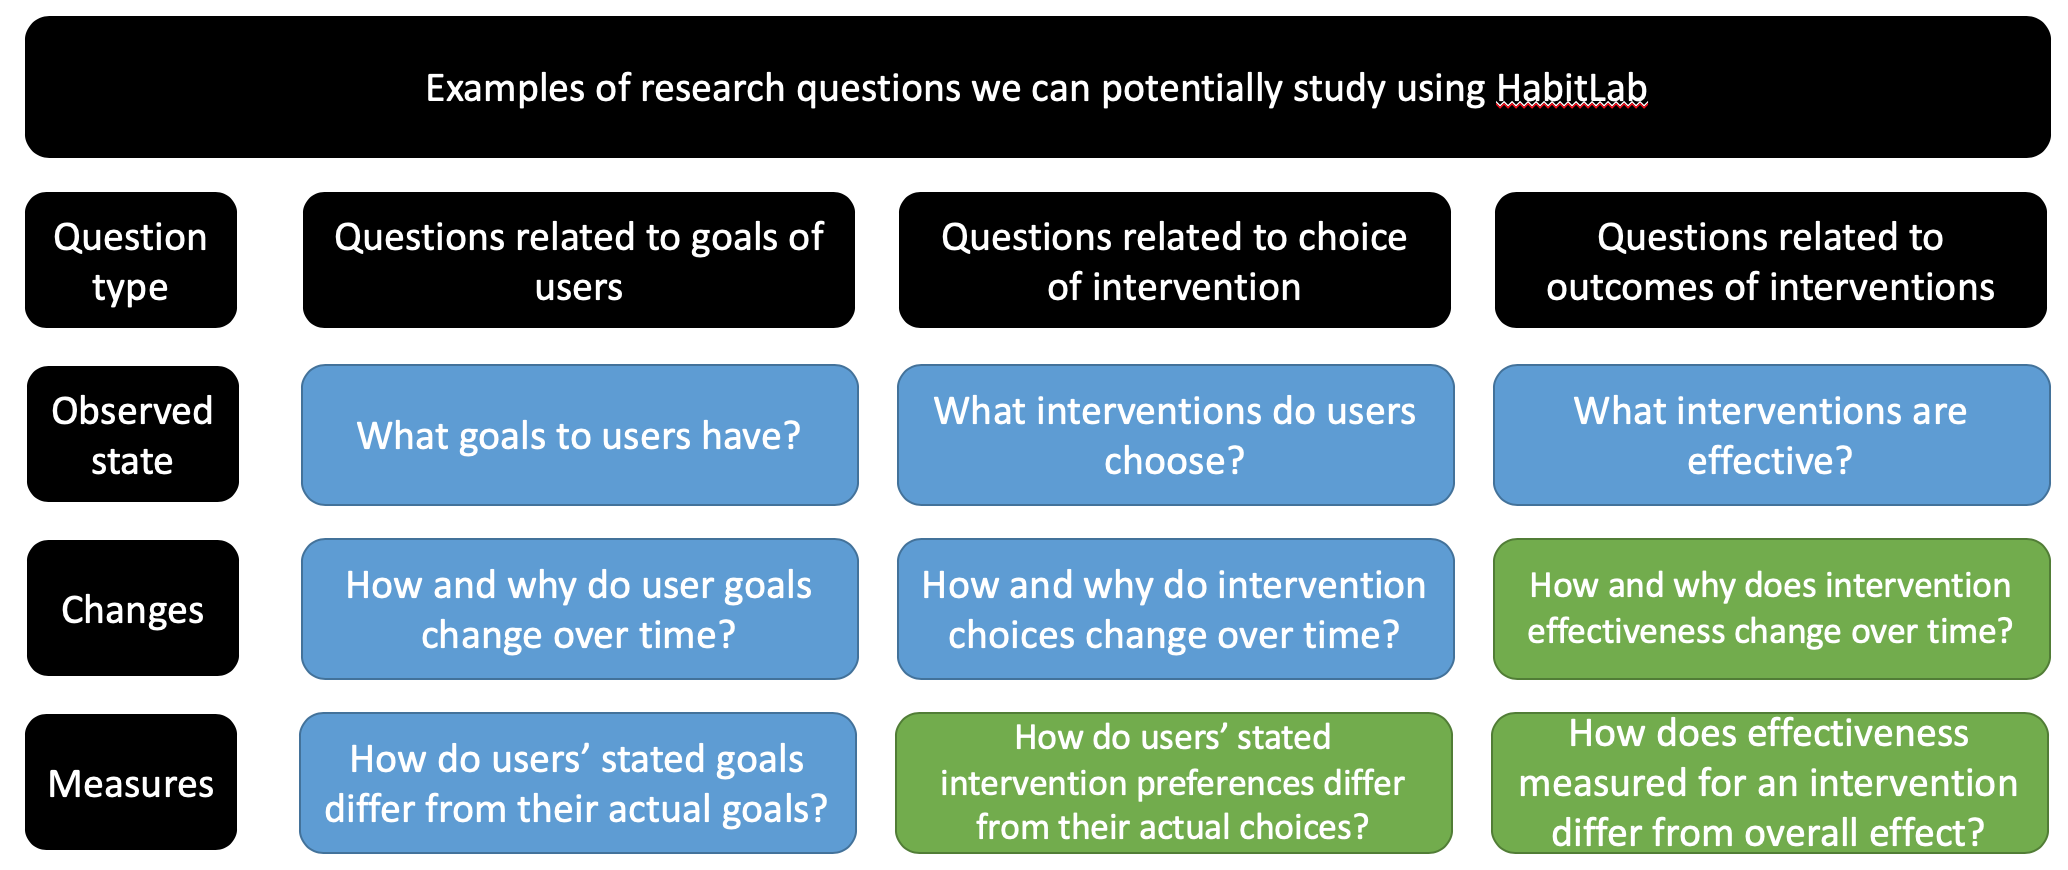
\includegraphics[width=\linewidth]{figuresI/researchquestions.png}
  \caption{Examples of research questions that can be studied with the HabitLab system and the general space of questions they occupy. Research questions we study in this thesis are shown in green.}
  \label{fig:researchquestions}
\end{figure}


There is a rich set of studies we can run with a tool such as HabitLab. The general paradigm is that users specify goals, interventions are deployed to help them achieve those goals, and we measure the outcomes of the interventions. At a high level, we can thus categorize the space of possible research studies that a platform such as HabitLab can conduct as below. A more detailed classification is shown in Figure~\ref{fig:researchquestions}.

\begin{enumerate}
\item Studies analyzing users' goals
\item Studies analyzing the choice of interventions to help users achieve those goals
\item Studies analyzing the outcomes of interventions
\end{enumerate}

We believe that the HabitLab system is uniquely well-suited for investigating the letter two classes of problems within behavior change. Specifically, it allows us to quickly test a variety of different choices of interventions -- as we can make arbitrary changes to websites, or show arbitrary overlays over the phone screen. Additionally, it also enables us to precisely measure the outcomes of the interventions -- specifically, we can directly observe the amount of time users spend on sites.

\section{Thesis Overview}

In this thesis we will first present the HabitLab system. Then we will describe a pair of studies conducted on the HabitLab system, which both study secondary effects that influence the intervention outcomes that we observe. %Then we will present three studies conducted on the HabitLab system: two analyzing the outcomes of interventions, and one study analyzing the choice of interventions to help users achieve those goals.

\subsection{HabitLab System Chapter}

We first describe the HabitLab system itself, the design process, the interventions, how we were able to amass a userbase of 12,000 daily active users via an in-the-wild deployment, and the demographics of those users.

\subsection{Intervention Rotation Chapter}

The first study we present asks whether the effectiveness of interventions decline over time. Prior literature suggests this is a possibility, as engagement-boosting novelty effects have been attested in numerous domains. We find that an intervention that is repeatedly presented does indeed decline in effectiveness over time, and that a strategy of rotating between different interventions helps boost effectiveness. This boost comes at the cost of increased attrition, which we find mostly to be due to incorrect mental models, as users are unaccustomed to interventions changing. A simple design helping explain the intervention rotation to users and give them a sense of control significantly reduces this resulting attrition.

\subsection{Time Redistribution Chapter}

The second study concerns itself with whether intervention outcomes are actually what we expect them to be looking at just the time spent on the targeted site or app. Prior literature suggests that willpower is limited, hence we may expect that reducing time on one app, site, or device may increase time spent on others. Other literature suggests that procrastination begets more procrastination by trapping us into a habit loop, hence we may expect that reducing time on one app, site, or device may reduce time spent on others. We find that in the case of site usage on browsers, reducing time on one site results in a reduction of time spent on others. In the case of app usage on mobile, we observe that reducing time on one app does not affect time on others. Likewise, in the case of devices, reducing time on one device does not affect time on others.

% The third study is about how users' preferences 

\subsection{Contributions}

The contributions of this thesis are:

\begin{enumerate}
\item HabitLab, a system for conducting in-the wild behavior change experiments online. It has been widely adopted with a 12,000 user install base across the browser and mobile platforms, showing that in-the-wild behavior change systems can be used to conduct large-scale experiments.
\item A set of studies conducted on HabitLab showing that static interventions decline in effectiveness over time, and that rotating interventions can improve their effectiveness.
\item A set of studies conducted on HabitLab showing that interventions can sometimes have beneficial secondary effects, reducing time spent on non-targeted sites.
\end{enumerate}

% our contributions in this thesis are

These studies show that our paradigm of in-the-wild experimentation, as realized in the domain of online behavior change via the HabitLab, can work to find novel insights about behavior change systems. We hope this work can help designers build better systems for online behavior change, and promote analogous in-the-wild experimentation in other behavior change domains.





\chapter{Related Work}

%\msb{start with an orienting paragraph. what are we going to cover in this chapter, and why? and, what's the roadmap?}

%\msb{the general role of a RW chapter is to cover the related work that sets up the context of your thesis. So, material that is relevant across all your chapters should show up here. Material that is specific to a single paper (e.g., rotation) should be in its respective chapter} \geza{done}

%\msb{A section I don't see here, but should be here: a thorough survey of behavior change systems. What is the design space of such tools? What is the state of the art? How does HabitLab draw on those tools, and how does it innovate?} \geza{done}

In this chapter we will cover work in sociotechnical systems, psychology, and behavioral economics related to behavior change and persuasive technology. We will begin with theoretical frameworks and taxonomies about behavior change, discuss examples of behavior change systems, discuss various tools which behavior change systems make use of, and finally explore the causes of attrition and why behavior change systems fail.

%----------------------------
% RQ
\section{Behavior Change Theories}
%The field of persuasive technology studies how technology can be used to influence behavior~\cite{fogg2002persuasive}. Persuasive technology systems have been successful in promoting behaviors such as sustainable resource usage~\cite{froehlich2009ubigreen}, fitness~\cite{consolvo2008activity}, sleep~\cite{kay2012lullaby,choe2011opportunities}, healthy eating~\cite{noronha2011platemate,epstein2016crumbs}, stress management~\cite{adams2014towards,sanches2010mind}, smoking cessation~\cite{paay2015personal}, and productivity~\cite{whittaker2016don, kim2016timeaware}. One common framework of behavior change is the B=MAT model~\cite{fogg2002persuasive}, which states that desired behaviors result when motivation, ability, and a trigger (a call to action) are all present. Another framework of habit change is the habit loop~\cite{eyal2014hooked}, which tells us that designs can build habits via a repeated process of displaying a trigger, having the user take an action, providing a reward, and having the user invest in the system.

\subsubsection{Theoretical Frameworks for Behavior Change}

%\msb{I don't really see the point of section headers for so few paragraphs. instead, just use strong topic sentences} \geza{done}

The field of persuasive technology studies how technology can be used to influence behavior~\cite{fogg2002persuasive}.
 There are a number of theoretical frameworks describing behavior change systems. B=MAT is a popular framework of behavioral change~\cite{fogg2002persuasive}, which demonstrates that systems can focus on three elements---motivation, ability, and a trigger (a call to action)---to produce behavior change. The habit loop is another framework for building habits~\cite{eyal2014hooked}, stating that systems can build habits through an iterated process of displaying a trigger, prompting the user to take an action, giving out a reward, and helping the user to invest in the system.

\subsubsection{Taxonomies of Behavior Change}

A number of taxonomies characterize the design space of interventions, both general~\cite{michie2013behavior, behaviourchangewheel, abraham2008taxonomy, dolanmindspace} and domain-specific~\cite{hardeman2000interventions, west2010behavior}. Michie's behavior change taxonomy lists 93 techniques for behavior change, clustered according to the cognitive phenomenon they target~\cite{michie2013behavior}. Systems have investigated effects of these techniques individually, such as using ``cheating'' to support lapse management~\cite{agapie2016staying}, using different framings to present results~\cite{kim2016timeaware}, or setting goals and plans~\cite{agapie2016plansourcing}.

\section{Behavior Change Systems}

Persuasive technology systems have been successful in promoting behaviors such as sustainable resource usage~\cite{froehlich2009ubigreen}, fitness~\cite{consolvo2008activity}, sleep~\cite{kay2012lullaby,choe2011opportunities}, healthy eating~\cite{noronha2011platemate,epstein2016crumbs}, stress management~\cite{adams2014towards,sanches2010mind}, smoking cessation~\cite{paay2015personal}, and productivity~\cite{whittaker2016don, kim2016timeaware}.

They can operate on many different platforms, such as the web or mobile devices. Web-based systems promote a behavior change goals including classroom engagement~\cite{anderson2014engaging, anderson2013steering}, psychology therapy~\cite{doi:10.1080/15228830802094429} and healthy habits~\cite{cugelman2013gamification, lyons2014behavior}. In parallel, a number of studies focused on mobile-based interventions~\cite{paredes2014poptherapy, RILEY201567, FJELDSOE2009165, Whittaker09, info:doi/10.2196/mhealth.4160}. For instance, MyBehavior, a mobile phone app, was built to track physical activities of the users and to provide personalized suggestions that are tailored to the users' historical behavioral data~\cite{info:doi/10.2196/mhealth.4160}. Similarly, PopTherapy is a mobile phone app that studied micro-interventions for coping with stress~\cite{paredes2014poptherapy}.

\subsubsection{Socialtechnical Systems for Behavior Change}

People use a variety of sociotechnical systems to support behavior change, including forums~\cite{eysenbach2004health, chancellornorms}, social sharing~\cite{poirier2012social, Chung:2016:BNA:2818048.2819926, pina2017personal, Ko:2015:NGI:2675133.2675244}, personal informatics~\cite{li2010stage, Chung:2017:PTB:3025453.3025747}, and self-experimentation~\cite{Karkar:2017:TFS:3025453.3025480}. People use behavior change forums to gain social support~\cite{hong2012outcomes} -- meeting social needs such as approval and esteem~\cite{kaplan1977social}. They do so by providing users with information and advice~\cite{hong2012outcomes}, and establishing norms~\cite{chancellornorms}. They also facilitate social comparisons~\cite{davison2000talks} which influence behaviors, as social comparison theory states that users seek to bring their behaviors in line with norms~\cite{festinger1954theory}. Communities also help users find others with similar experiences~\cite{huh2014health} who can help them through the process of recovering and adapting to changes~\cite{newman2011s}. Social sharing~\cite{poirier2012social, richardson2010online} works by helping users receive support through social interactions, and encouraging accountability~\cite{epstein2015nobody}. Personal informatics support behavior change through stages of preparation, collection, integration, reflection, and action~\cite{li2010stage}. The theory of lived informatics~\cite{epstein2015lived} adds additional stages where users choose tracking tools, and alternate between lapsing and resuming their tracking behaviors. % HabitLab combines personal informatics and self-experimentation to support behavior change. Our study draws on lived informatics by evaluating whether rotating interventions is an effective strategy to combat lapses such as ignoring interventions or uninstalling.

% Of course, sociotechnical systems may also have deleterious effects --- communities may set unhealthy norms such as encouraging eating disorders~\cite{chancellornorms}, and social sharing can cause anxiety~\cite{munson2010happier}, impression management concerns~\cite{consolvo2014designing}, and make users unwilling to set goals~\cite{munson2015effects}.

% \msb{Can you pull this together into a summary of what we draw from this literature and how it influences HabitLab or our study?}

\subsubsection{Online Behavior Change}

One major topic inspiring our work is users' desires to curb or control their time spent on social media sites. People pressure themselves to, and often do, make efforts to reduce their time spent on social media sites such as Facebook and Twitter~\cite{Sleeper:2015:ILI:2675133.2675193,schoenebeck2014giving}. Yet this is difficult because users turn to social media to address their need to belong, the need for self-presentation, the need for self-esteem~\cite{nadkarni2012people}, the need for entertainment and gratification ~\cite{raacke2008myspace}, and self-affirmation ~\cite{toma2013self}. Whether social media use improves well-being is a complex question depending on the nature of the engagement ~\cite{uysal2013mediating, marche2012facebook, lin2015emotional, kim2011facebook, muise2009more, sagioglou2014facebook, tandoc2015facebook}, but thanks to instant gratification and sites' use of gamification~\cite{chou2015actionable, zichermann2011gamification, huotari2012defining} and behavior design techniques~\cite{fogg2002persuasive, eyal2014hooked} to drive engagement, users keep coming back to the point that some consider it an addiction~\cite{andreassen2012development, ryan2014uses, tang2016personality, turel2014examination}. %Furthermore, social media sites make heavy use of gamification to drive engagement on their sites~\cite{chou2015actionable, zichermann2011gamification, huotari2012defining}, and are cited as successful applications of behavior change theories~\cite{fogg2002persuasive, eyal2014hooked}.} %Furthermore, social media sites are designed to maximize user engagement, with features closely following gamification strategies~\cite{chou2015actionable} and behavior change theories~\cite{fogg2002persuasive, eyal2014hooked}.}

\section{Tools Used By Behavior Change Systems}

Researchers in behavioral economics and related fields have developed a number of tools which are useful for building behavior change systems. Gamification, which introduces triggers, investment, rewards, and game-like elements to motivate behavior change, and personalization are a pair of tools which are often used to boost the effectiveness of behavior change systems. Another one of these tools is \textit{choice architectures}, or ways to structure choices to influence behaviors.

\subsubsection{Gamification}

Much previous work has focused on gamification as an approach to design behavior change systems~\cite{deterding2011game}. Gamification has been shown to have positive effects on engagement and outcomes in behavior-change contexts such as promoting healthy habits~\cite{cugelman2013gamification, lyons2014behavior} and improving  educational engagement~\cite{anderson2013steering, anderson2014engaging}, though effectiveness varies depending on the context and design~\cite{6758978}. % Popular online services such as Facebook and LinkedIn make heavy use of gamification to drive engagement on their sites~\cite{chou2015actionable, zichermann2011gamification, huotari2012defining}.


\subsubsection{Personalization}

A recent trend in behavior change systems has been the concept of personalizing interventions. Such systems explore several possible strategies using techniques such as multi-armed bandits to find the intervention that is most effective for the user~\cite{paredes2014poptherapy, rabbi2014automated}. For example, PopTherapy demonstrated personalized messaging could be found through such techniques~\cite{paredes2014poptherapy}. Likewise, HeartSteps conducted tens or hundreds of micro-randomized trials on users~\cite{doi:10.1111/j.1740-9713.2015.00863.x}.  % When multi-armed bandits are just beginning to get feedback from a user, they will try out several different interventions to see what works. This exploration has the effect of rotation, but the amount of rotation declines as the bandit begins to personalize. %In this paper, we examine the contrarian assertion that perhaps rotation should be maintained to sustain novelty even after the multi-armed bandit is aware of which intervention is most effective for the user.

\subsubsection{Choice architectures}

The field of behavioral economics has developed a number of theoretical frameworks for how to present choices to influence people's choices, known as choice architectures~\cite{thaler1980toward, thaler2009nudge, johnson2012beyond}. One of the best-known choice architectures is defaults -- the choice made if the user does not make an active choice -- which work by exploiting the status-quo bias~\cite{samuelson1988status}. Defaults have been found to be effective in numerous behavior change contexts, including increasing organ donations~\cite{johnson2003defaults}, encouraging saving for retirement~\cite{cronqvist2004design, madrian2001power}, and influencing choice of insurance plans~\cite{johnson1993framing}. Other examples of effective, widely deployed choice architectures include limiting the number of choices~\cite{cronqvist2004design, kling2008misperception}, sorting choices~\cite{lynch2000wine}, grouping choices~\cite{fox2005subjective}, and simplifying choice attributes to be more easily interpretable~\cite{peters2009bringing, soll2013consumer}. Some choice architectures are designed explicitly for interactive behavior change contexts where users repeatedly make choices, such as Enhanced Active Choice, which provides users with choices while attempting to steer them towards the desired one~\cite{keller2011enhanced}.

%\subsection{Choice Architectures to Reduce Myopic Choices}

A number of choice architectures have been developed to combat our bias towards myopic choices, aversion to uncertainty, and lead us to choices that have better long-term outcomes~\cite{johnson2012beyond}. If the user is choosing between short-term benefits and longer-term benefits, one strategy is to make the long-term outcomes of the choice more salient in the short term~\cite{weber2007asymmetric, soman2005psychology}. In cases where there are a large number of uncertain outcomes and we wish to encourage satisficing -- that is, choosing an acceptable option sooner rather than waiting for a hypothetical future optimal choice -- we can focus attention on the second-best outcomes~\cite{shu2008future}. This strategy of satisficing can both lead users to decide faster, and leave them happier with their choices~\cite{iyengar2006doing}. We can also combat procrastination resulting from users' tendency to be overly optimistic about future opportunity windows by explicitly enforcing limited opportunity windows~\cite{o1998procrastination}.




% One of the most comprehensive investigations we
% identified is a recent meta-analysis of 85 studies by
% Webb et al. (2010) that found interventions that were
% strongly based in theory had greater impact than those
% that were not, and interventions that incorporated more
% behavior change techniques tended to have larger
% effects than interventions that incorporated fewer techniques

% Within the CSCW community, behavior change has been an active area of research. One major topic inspiring our work is users' desires to curb or control their time spent on social media sites. People pressure themselves to, and often do, make efforts to reduce their time spent on social media sites such as Facebook and Twitter~\cite{Sleeper:2015:ILI:2675133.2675193,schoenebeck2014giving}. This paper builds on this literature, contributing studies of how people might become more effective at this goal. Sociotechnical systems are also locations where people discuss behavior change~\cite{chancellornorms}, and find social support~\cite{Ko:2015:NGI:2675133.2675244, Chung:2017:PTB:3025453.3025747}. Behavior change often requires self-tracking, self-experimentation, and personal informatics~\cite{Karkar:2017:TFS:3025453.3025480}, leading to opportunities to share data and progress with trusted others~\cite{Chung:2016:BNA:2818048.2819926, pina2017personal}.


% datu2012does

% Social media is particularly addictive be

% \rev{expanded the related work discussion on sociotechnical theories. list the theories driving these papers. social support cscw theories. why people use forums for behavior change support what role do other people play in driving your behavior change. collective exercise. why are social media particularly hard to manage your behavior with why is social media addictive.}

% \rev{festinger's social comparison theory postulated that social behaviors could be predicted largely on the basis of the assumption that individuals seek to have and maintain a sense of normalcy and accuracy about the world}

% http://journals.sagepub.com/doi/pdf/10.1177/1524839911405850
% Harnessing Social Media for Health Promotion and Behavior Change

% \rev{Communities and collaborative support can help achieve behavior change goals. }




%Attrition is a major challenge in behavior change systems: a metastudy of eHealth interventions found that an attrition rate around 99\% over a 12-week period is normal~\cite{eysenbach2005law}. %Similarly, attrition may also exist in our online behavior change system with rotating interventions. Studies in behavior changes systems report attrition of users over time. 
%Likewise, the number of users in a stress-coping mobile application declined in a steady rate through the study~\cite{paredes2014poptherapy}. 


% The challenges of static interventions, and the rising wave of personalization systems, call into focus: would a rotation strategy work? Or is it a weak palliative with little discernible effect? This led to our research question:

%\begin{resques}[RQ]
%Can a strategy of rotating interventions produce more effective behavior change systems?
%Does rotating interventions is helpful in increasing effectiveness and lowering attrition in online behavior changes systems?}
%\end{resques}

%----------------------------
% HYP


%----------------------------
% Below this line is
% Archived materials
%----------------------------

% Todo:

%----------------------------
% Opening

% The field of persuasive technology studies how technology can be used to influence behavior~\cite{Fogg:2002:PTU:764008.763957}. Persuasive technology systems have been successful in promoting behaviors such as sustainable resource usage~\cite{froehlich2009ubigreen}, fitness~\cite{consolvo2008activity}, sleep~\cite{kay2012lullaby,choe2011opportunities}, healthy eating~\cite{noronha2011platemate,epstein2016crumbs}, stress management~\cite{adams2014towards,sanches2010mind}, smoking cessation~\cite{paay2015personal}, and productivity~\cite{whittaker2016don, kim2016timeaware}. Computer tailored interventions - one of the most widely studied persuasive technology, are often implemented based on a static system (a single intervention)~\cite{stayfocusd, leechblock, selfcontrolapp, focusbooster} or on a dynamic system that keeps rotating new interventions in a designed sequence~\cite{paredes2014poptherapy, rabbi2014automated, Kaptein2013, Kaptein:2011:MBA:1978942.1978990}. However, we do not really understand the effectiveness of intervention over time nor the possible influences of rotating interventions on effectiveness and attrition of behavior change systems. Instead of treating the computer tailored behavior change systems as a black-box to increase effectiveness in a short-term, we aim for a deep understanding about the behavior changing systems and building a system that can maintain high effectiveness in a long-run, which are crucial for proving the efficacy of a behavior change system~\cite{Klasnja:2011:ETH:1978942.1979396}.

% %----------------------------
% \subsection{Learning the effectiveness and attrition}
% A number of behavior change systems have proven helpful in increasing the effectiveness of an intervention~\cite{krebs2010meta, kaptein2015personalizing}. They often involve rotating interventions algorithmically such as multi-armed bandits~\cite{paredes2014poptherapy, rabbi2014automated}.  However, a consequence of using multi-armed bandits algorithm is that there is a high rotation rate among interventions in the beginning (during exploration). During this process, it starts showing the same intervention with increasing probablity (during exploitation)~\cite{AUDIBERT20091876}. Prior work suggests that the effectiveness of showing a constant intervention over time cannot be maintained indefinitely~\cite{Hiniker:2016:MDE:2858036.2858403, riekert2013handbook}. Meanwhile, randomly rotating between new interventions on personal devices such as \textit{Fitbit} has found an increase the effectiveness of interventions~\cite{doi:10.1111/j.1740-9713.2015.00863.x}. 

% Furthermore, learning the attrition of behavior change systems is important. Attrition (or dropout) has been a problem among participants in health research~\cite{Eysenbach2005attrition}. For example, persuasive systems built for weight-control report have shown increased attrition rates in longitudinal studies~\cite{Bernier1986}. To the best of our best knowledge, although dropping-out of users from the study has been reported~\cite{paredes2014poptherapy}, the increments in attrition has not been discussed in detail or quantified.

% Currenty, studies in health are investigating in similiar concepts: Micro-Randomised Trial (MRT) and Just-in-Time Adaptive Interventions (JITAIs)~\cite{MRT2015Klasnja}. Contrary to traditional Randomized Control Trial (RCT) which randomizes all the participants in the beginning, MRT and JITAIs are experimental design conceptions that randomize particpants in a micro-steps, in which participants can be exposed to different interventions. Our findings about attrition of rotating interventions can potentially contribute to health science research.

% In summary, there is a need for taking the wearout effect among various interventions into account when quantifying the effectiveness of single intervention and rotating interventions. The results would greatly help with designing a better persuasive system for behavior changes. Additionally, research on attrition of interventions could provide useful insights into building effective behavior change systems in the long-run. Thus, we proposed our research questions in the following: (RQ1,2,3)

% %----------------------------
% \subsection{Combating with attrition}
% Learning to build a behavior change system that compensates for the attrition has become an imperative. Behavior changes are often long-term complex processes that require years of efforts to accomplish on one\'s will~\cite{prochaska1997transtheoretical}. Steady drop-out rate in intervention systems exists in previous studies of personal behavior change systems~\cite{paredes2014poptherapy, krebs2010meta}. Drop-outs will not only result in the termination of the intervention system but also in a decrease in efficacy of such system~\cite{Klasnja:2011:ETH:1978942.1979396}. Thus, lowering the attrition in the long-run becomes a crucial step for making an effective behavior change systems. However, there has been little research on improving existing online intervention systems to lower the attrition.

% Outside the field of persuasive technology, lowering the attrition has been \textit{de facto} studied for years. Known as the IKEA effect, studies have shown that participants tend to value more on self-made products~\cite{NORTON2012453}. The attrition might be decreased if the participants are actively contributed to building the intervention systems. Meanwhile, various methods have been proposed in minimizing attrition in longitudinal health research including incentives, reminders and follow-up interviews~\cite{BOYS2003363, RIBISL19961}. Using a combination of different retention strategies also appears to lower the attrition~\cite{ROBINSON20151481}. Surprisingly, participants also show steady engagement in studies if opt-in/opt-out option is provided~\cite{doi:10.1080/13645570701334084}. Framing the interventions is also found to be useful to enhance effectiveness of a behavior change system~\cite{kim2016timeaware}.

% Taken together, previous literature has painted a picture where lowering the attrition is necessary to designing an effective intervention system. In economics and health studies, numerous studies have shown ways to decrease attrition of participants over time. This observation motivates our research questions: (RQ4,5,6)



% \subsection{Interface Design and Users Behavior}

% H4: Users who enable or disable interventions during the beginning are less likely to attrition.
% Cite something in psyc literatures that prove IKEA effect, and demostrate root cause of it. [cite needed here.] 
% Talke about IKEA effect in a systematic way. Present some concrete results here, how the IKEA, "do-it-youself" help making more and more costumers engaged and love their products. [cite needed here.] 
% Cite any researches done in the HCI domain field, if any. Talk about how design the system in embed IKEA effect will reduct attrition. [cite needed here.]

% H5: Reminding them how system work will improve user's mental model and reduce attrition.
% Reminding system is everywhere, and they are here for a reason. Reminding system works, improve efficacy, show concrete results here[cite needed here.] 
% Mental model formation of users [cite needed here.]  How is mental model related to attrition in other literature [cite needed here.] 
% Given concrete examples when reminding system work in increasing user engagement and reduce drop out rate.

% H6: Users feel of control and attrition over time. Given them opt-out option will actually reduct attrition.
% Cite peoples natural inclination of control things [cite needed here.]. 
% Cite literatures where user opt-in/opt-out actually will reduce attrition in a long run[cite needed here.], in average. because when user opt-out, then should be count as a negtive instance. But in avrage, the hypothesis we are proposing is, the attrition will go down. 
% Cite literatures outside HCI, when user does not feel of control, they will drop out. The downside of rotating interventions quickly[cite needed here.]. 
% We can also cite previous researches show user dropout[cite needed here.]. 
% We suspect that it might be due to lack of control. Thus, we propose this hypothesis.

% In health fields, 

% Probably from one of the grant proposals or so

% this one shows existence of novelty effects \cite{krebs2010meta}

% https://www.sciencedirect.com/science/article/pii/S0091743510002318

% poptherapy

%Despite numerous previous research in computer-tailored interventions system using algorithms such as multi-armed bandits, the existing literatures mainly focus on the comparisons of the effectiveness between the algorithmic system and other non-algorithmic system such as showing static interventions or selecting randomly - there are few direct investigations discuss that effects of the algorithmic intervention system in a long-run. Users might feel fatigue of novelty - alternating between different interventions and feel lack of control which might lead to aversion to the algorithm. In our study, we analyze not only the effectiveness of computer-tailored interventions system but also the attrition rate of end users. Additionally, majority of previous works on computer-tailored interventions system focus on health issue and very few of them touches on on-line productivity.

%In health fields, Paredes et al created a computer-aid intervention system, which used multi-armed bandits algorithm to help people to cope better with stress\cite{paredes2014poptherapy}. They found that participants statistically significantly lowered the stress level after using their system. They also found that setting a hard constraint for exploration rate as 50\% and thus proposed that novelty would ensure the efficacy of their system. However, they did not consider the decline of effectiveness of intervention over time in any experiment. The attenuation of intervention effectiveness was proved in many previous studies\cite{krebs2010meta}. On the other hand, we found that constantly switching between interventions might have negative consequences. For instance, the users might be fatigued and feel lack of control if the users saw different interventions frequently.

%Rabbi et al developed a system that encouraged users for more healthy behavior changes by displaying messages in a mobile health app\cite{rabbi2014automated}. They used multi-armed bandits algorithm to personalize contextual suggestions and found the adaptive algorithm more actionable. However, they only deployed their research in small recruited groups as a short-term process in which the relation between the adaptive algorithm and attrition rate was not considered in a long-run setting. 

%Similarly, Kerbs et al wrote a meta-analysis study of 88 computer-tailored interventions that were designed for health behavior changes in four different groups: smoking cessation, physical activity, eating a healthy diet, and receiving regular mammography screening \cite{krebs2010meta}. They found clinical and statistical significances in effectiveness for each of four behaviors. They also found the efficacy of interventions decreased over time unless the interventions were dynamically changing, which introduced novelty. Furthermore, they showed that greater effects for the novelty effect were seen in the long-run as well. Although they rigorously proved the existence of novelty effect (algorithmically alternating between different interventions) in computer-aid intervention system in health studies, they did not consider the possible negative effects might be come with this alternation between interventions, which we found in our study. The point of measuring the attrition rate in a long-run was crucial for health behavior change in HCI research because it increase the validity of your research, as Klasanja et al pointed out that a longitudinal study was needed for proving the efficacy\cite{Klasnja:2011:ETH:1978942.1979396}.

%In technology fields, Kaptein and Markopoulos analyzed the importance of implicit profiling in various persuasive systems: Persuasive Messaging System(PMS) and Persuasion profiling in e-commerce\cite{kaptein2015personalizing}. They found that dynamically profiling users using the adaptive algorithm (multi-armed bandits algorithm) over-performed any other persuasive system, including pre-selecting a fixed persuasive system by educated crowds. We found similar trends as we discovered that alternating between different interventions could increase the effectiveness of our tool. However, Similar to previous works in health, they did not consider how the novelty might affect the attrition rate of end-users as well.


%----------------------------
% RQ
%\section{Behavior Change and Motivation}

%\msb{Take a pass through this section and remove phrases like "Studies show X" or "Researchers have found X". It's weak writing. Instead just state the claim X. Like instead of "Researchers have found that hotdogs are tasty [cite].", just write "Hotdogs are tasty [cite]." I removed several already.}

% The field of persuasive technology studies how technology can be used to influence behavior~\cite{fogg2002persuasive}. Persuasive technology systems have been successful in promoting behaviors such as sustainable resource usage~\cite{froehlich2009ubigreen}, fitness~\cite{consolvo2008activity}, sleep~\cite{kay2012lullaby,choe2011opportunities}, healthy eating~\cite{noronha2011platemate,epstein2016crumbs}, stress management~\cite{adams2014towards,sanches2010mind}, smoking cessation~\cite{paay2015personal}, and productivity~\cite{whittaker2016don, kim2016timeaware}. An influential framework of behavior change is the B=MAT model~\cite{fogg2002persuasive}, which states that desired behaviors result when motivation, ability, and a trigger (a call to action) are all present. Another framework of habit change is the habit loop~\cite{eyal2014hooked}, which tells us that designs can build habits via a repeated process of displaying a trigger, having the user take an action, providing a reward, and having the user invest in the system.

%\msb{what is lifestyle? it looks like sleep? is this capturing something else? I don't think lifestyle is the right word here}


%\msb{subsection titles for single paragraphs are unnecessary in related work; I'm cutting them}

\section{Measuring Overall Effectiveness}

% Persuasive technologies on computers and mobile phones can help support behavior change. Researchers have developed web-based systems to promote a variety of behavior change goals, including psycho-therapeutic interventions~\cite{doi:10.1080/15228830802094429}, promoting healthy habits~\cite{cugelman2013gamification, lyons2014behavior} and improving educational engagement~\cite{anderson2013steering, anderson2014engaging}. In parallel, a number of studies focus on mobile-based interventions~\cite{paredes2014poptherapy, doi:10.1111/j.1740-9713.2015.00863.x, RILEY201567, anderson2014engaging, FJELDSOE2009165, Whittaker09}. For example, PopTherapy studied micro-interventions for coping with stress using mobile devices~\cite{paredes2014poptherapy}. Likewise, HeartSteps developed an application on mobile phones to promote promote physical activities for individuals~\cite{doi:10.1111/j.1740-9713.2015.00863.x}. % For HabitLab, we developed a version for computers as well as a version for mobile phones. Our study studies user behaviors by evaluating real-time data from both platforms.

% These persuasive technologies have produced measurable beneficial effects. Web-based systems promote a behavior change goals including classroom engagement~\cite{anderson2014engaging, anderson2013steering}, psychology therapy~\cite{doi:10.1080/15228830802094429} and heathy habits~\cite{cugelman2013gamification, lyons2014behavior}. In parallel, a number of studies focused on mobile-based interventions~\cite{paredes2014poptherapy, RILEY201567, FJELDSOE2009165, Whittaker09, info:doi/10.2196/mhealth.4160}. \msb{I don't understand how this paragraph is different from the prior one. Didn't the prior one just list a bunch of domains for behavior change systems?} For instance, MyBehavior, an app on mobile phone, was built to track physical activities of the users and to provide personalized suggestions that are tailored to the users historical behavioral data~\cite{info:doi/10.2196/mhealth.4160}. Similarly, PopTherapy is an a mobile phone application that studied micro-interventions for coping with stress~\cite{paredes2014poptherapy}.

% Measuring the effectiveness of a persuasive system remains a major challenge in behavior change systems design. While behavior change systems can be effective during the experiments~\cite{doi:10.1080/15228830802094429, Cuijpers2008, info:doi/10.2196/jmir.1376}, many review papers are more restrained in whether behavior change systems remain effective outside the studies~\cite{doi:10.1111/j.1467-789X.2009.00646.x, 10.1371/journal.pmed.1000387, NORMAN2007336, 10.1007/978-3-319-07127-5_11}. The critique holds that behavior changes are long, complex processes, and the effectiveness of a system is hard to measure in a short period of time~\cite{prochaska1997transtheoretical}. For instance, an intervention promoting healthy habits, which is effective in changing participants eating habits, might reduce their physical activities which are not measured in the experiment~\cite{COTTER2014243}. Likewise, a system promoting physical activities might have no knowledge on participants' eating habits~\cite{doi:10.1111/j.1740-9713.2015.00863.x}. With interventions on both the computer and the mobile device for each user, our study draws on lived informatics by evaluating the efficacy of productivity interventions in the context of a more complete ecosystem which includes both computers and mobile devices.

Measuring the effectiveness of a persuasive system remains a major challenge in the design of behavior change systems. While behavior change systems can be effective during experiments~\cite{doi:10.1080/15228830802094429, Cuijpers2008, info:doi/10.2196/jmir.1376}, many review papers are more restrained in whether behavior change systems remain effective outside studies and bring longitudinal behavioral change~\cite{doi:10.1111/j.1467-789X.2009.00646.x, 10.1371/journal.pmed.1000387, NORMAN2007336, 10.1007/978-3-319-07127-5_11}. Because behavior changes are long and complex processes, the efficacy of a persuasive system is often difficult to measure~\cite{prochaska1997transtheoretical}. For instance, an intervention promoting healthy habits, which was effective in changing participants' eating habits, might reduce their physical activities, which were not measured in the experiment~\cite{COTTER2014243}. Likewise, a system promoting increased physical activity may be unable to observe effects on participants' eating habits~\cite{doi:10.1111/j.1740-9713.2015.00863.x}. Compared to prior work, our study examines these spillover effects in the context of a more complete ecosystem, including both desktop browsers and mobile devices. % \msb{I don't know what this means}.  \msb{use this paper in the intro to motivate the redistribution hypothesis}

\subsection{Multi-Device Usage}

Cyberslacking, referred to as non-work-related computing, is the use of Internet and mobile technology during work hours for personal purposes~\cite{VITAK20111751,PEE2008120, Pamela2004, lim2002}. One study found that employees spent at least one hour on non-work-related activities during a regular work day~\cite{VITAK20111751}. Researchers also reported that non-work-related Internet usage comprises approximately 30\%--50\% of total usage~\cite{RESTUBOG2011247,JAMALUDDIN2015495}. %  \msb{this sentence seems disconnected from everything that came before. why is it here?}.

%\subsection{The Vicious Cycle of Procrastination}

Unproductive time begets further unproductive time. For example, increased time spent online can increase sleep debt, which in turn leads to more time spent online \cite{Mark:2016:SDS:2858036.2858437}. Likewise, the Hook Model claims that many of the most addictive online sites use a cycle of investment techniques to keep users coming back---for example, making a post on Facebook may result in future notifications, which will in turn will get the user to come back and make more posts~\cite{eyal2014hooked}. Finally, sites such as Facebook, Reddit, Twitter, and Buzzfeed are filled with links to each others' content, so it may be the case that increasing usage of one will increase usage of others. If productivity interventions are able to break this vicious cycle of procrastination for one application, they may actually reduce time spent on other unproductive applications as well.

% The importance of understanding the effectiveness of productivity interventions in a complete ecosystem and the rising awareness of unproductive time spent on mobile devices call into focus: would productivity interventions reduce net unproductive time? Or is it a weak palliative with little discernible effect? This led to our research question:

%\begin{resques}[RQ]
%Do productivity interventions reduce net unproductive time, or just redistribute it to other applications, sites, and devices?
%Does rotating interventions is helpful in increasing effectiveness and lowering attrition in online behavior changes systems?}
%\end{resques}

\subsection{Distribution Of Unproductive Time}

%\msb{Same, remove "Studies show X" or "Researchers have found X". } \goli{done}

In this section, we will examine related studies in behavior change systems to develop testable hypotheses regarding the research question.

%\subsection{Intra-device}

Multitasking has become ubiquitous in today's workplaces~\cite{Appelbaum2016, mark2015multitasking, CARRIER2009483}. Multitasking is both essential and unavoidable in the workplace~\cite{freedman2007, mark2008cost}, and it takes 11 minutes on average before people switch to a new task~\cite{dabbish2011keep}. 
% The nature of multitasking in the workspace presents a challenge for designing effective productivity interventions in the face of multiple tasks. %concurrent tasks.
%Researchers also reported multi-tasking on computers is a required skill in employment recruiting nowadays. The study pointed out that an internet-based search of the terms "job description" and "multitasking", by using Google, had over 1.2 million results~\cite{Appelbaum2016}. 
% However, the nature of multitasking in the workspace increases the difficulty of designing effective productivity interventions when there are multiple concurrent tasks. % When one goal increases productivity via an intervention, people might redistribute their unproductive time to other goals instead. \msb{this claim is just thrown out without citations and dropped. either back it up or remove it}
% \msb{inconsistent throughout: is it multitasking or multi-tasking?}

% Persuasive systems often bring the intended behavioral changes (e.g.~\cite{doi:10.1080/15228830802094429,cugelman2013gamification, lyons2014behavior,anderson2013steering, anderson2014engaging}). These results suggest that, at the very least, HabitLab can reduce the time spent on unproductive activities. \msb{I don't see why this paragraph is relevant at all to developing H1 or H2. cut?}

% However, the time spent on unproductive activities might be redistributed elsewhere. While scholars found that persuasive technologies could produce positive outcomes, others worried that interventions could result in negative consequences which might promote users to adopt the opposite target behavior~\cite{10.1007/978-3-319-07127-5_11, 10.1007/978-3-319-31510-2_6}. For example, the tobacco industry sponsored anti-smoking campaign that supports parents to educate their children on risks of smoking could backfire, promoting some teens to light up~\cite{trove.nla.gov.au/work/31391712}. Similarly, researchers who study anti-bullying wristbands found that the wristband campaign increased the chances of bullying for the kids who wear it~\cite{antibullying}. \msb{No, these literatures don't suggest a redistribution hypothesis, it supports a sort of ``reverse effect'' hypothesis where the time on the targeted goal is increased rather than decreased}  This prompts our first hypothesis:
Studying behavior change effects across multiple devices is important: focusing on a single platform will myopically miss unproductive behaviors on other platforms. %because people distributed their unproductive behaviors across multiple People spend time on unproductive activities with computers and mobile phones. 
Attention is fragmented in both mobile and traditional desktop environments~\cite{socialmedia2010, mark2015multitasking}. The time spent on mobile devices has increased more rapidly than time on computers or TVs~\cite{multidevice, nielsen}. On the other hand, mobile applications have been regarded as substitutions of websites in many studies~\cite{10.1007/978-3-642-36516-4_7}. Large technology companies such as Facebook and Amazon have been focusing on user growth on mobile devices~\cite{socialmedia2010}.

However, interventions may result in unintended outcomes~\cite{trove.nla.gov.au/work/31391712, 10.1007/978-3-319-07127-5_11, 10.1007/978-3-319-31510-2_6}. Specifically, while some interventions may be highly effective at achieving the measured goal of a behavioral change system, they may reduce desired outcomes elsewhere~\cite{10.1007/978-3-319-07127-5_11}. In one health-related intervention, while the physical activity of participants increased, calorie intake also increased, working against the goal of promoting a healthy lifestyle~\cite{Blair1985}. Similarly, using peer pressure to build confidence for students at school would, in turn, lower their self-esteem which actually was opposite to the goal of augmenting confidence~\cite{10.1007/978-3-319-31510-2_6}.

\section{Motivation and User Choices}

Researchers in the field of behavioral economics have conducted numerous studies about users' motivation levels, how they change with time, and whether users can accurately predict their future motivation levels. Additionally, a number of \textit{choice architectures}, or ways to structure choices to influence behaviors, have been studied.

\subsection{Optimism vs Unrealistic Optimism}
Are users initially too optimistic and have unrealistic expectations? Or are they able to accurately judge their levels of self-control? Does optimism have positive or negative results in behavior-change contexts?

Optimism -- a generally positive and hopeful attitude towards their future abilities to change -- is generally considered to be beneficial in behavior change, and is considered to predict positive outcomes~\cite{davidson1997optimism}. Behavior-change literature makes a distinction between this optimism and unrealistic optimism -- where the subject underestimates their susceptibility to health problems -- which is considered to be detrimental towards behavior change outcomes~\cite{davidson1997optimism}.

In dieting contexts, users tend to overestimate their self-control abilities and have unrealistic expectations of their ability to lose weight~\cite{sparks1995perceived}. The level of participants' optimism -- how much they underestimate their ability to -- can be predicted based on survey questions related to their self-identity and theory of planned behavior. However, users differ in the levels to which they are optimistic~\cite{davidson1997optimism}.


\subsection{Short-Term Myopia vs Long-Term Goals}

Users often make short-term choices that conflict with their long-term goals, which often manifest themselves as inability to delay gratification, lack of self-control, procrastination, and addiction~\cite{loewenstein1992choice, shu2010procrastination}. These myopic choices can be attributed to a number of factors -- firstly, short-term benefits are more immediate and salient than long-term losses, leading us to discount future outcomes~\cite{ainslie2001breakdown, loewenstein1992choice, soman2005psychology}. The degree to which users place decreasing value on future outcomes has been studied in various economics experiments on intertemporal discounting~\cite{weber2007asymmetric}, and models such as hyperbolic discounting and subadditive discounting have been proposed to describe this bias in mathematical terms~\cite{ainslie1992hyperbolic, rubinstein2003economics, read2001time}.

Additionally, we are often certain of short-term benefits, while long-term effects such as life expectancy are less certain, so we discount the uncertain, long-term outcomes~\cite{payne2013life}, or end up considering only a desireable subset of possible outcomes~\cite{shu2008future, koehler1991explanation}. Optimism can also play a role in myopic choices, as we are often overly optimistic that we will not suffer from possible negative long-term consequences~\cite{kahneman1993timid, zauberman2005resource}.

\subsection{Choice architectures}

The field of behavioral economics has developed a number of theoretical frameworks for how to present choices to influence people's choices, known as choice architectures~\cite{thaler1980toward, thaler2009nudge, johnson2012beyond}. One of the best-known choice architectures is defaults -- the choice made if the user does not make an active choice -- which work by exploiting the status-quo bias~\cite{samuelson1988status}. Defaults have been found to be effective in numerous behavior change contexts, including increasing organ donations~\cite{johnson2003defaults}, encouraging saving for retirement~\cite{cronqvist2004design, madrian2001power}, and influencing choice of insurance plans~\cite{johnson1993framing}. Other examples of effective, widely deployed choice architectures include limiting the number of choices~\cite{cronqvist2004design, kling2008misperception}, sorting choices~\cite{lynch2000wine}, grouping choices~\cite{fox2005subjective}, and simplifying choice attributes to be more easily interpretable~\cite{peters2009bringing, soll2013consumer}. Some choice architectures are designed explicitly for interactive behavior change contexts where users repeatedly make choices, such as Enhanced Active Choice, which provides users with choices while attempting to steer them towards the desired one~\cite{keller2011enhanced}.

\subsection{Choice Architectures to Reduce Myopic Choices}

A number of choice architectures have been developed to combat our bias towards myopic choices, aversion to uncertainty, and lead us to choices that have better long-term outcomes~\cite{johnson2012beyond}. If the user is choosing between short-term benefits and longer-term benefits, one strategy is to make the long-term outcomes of the choice more salient in the short term~\cite{weber2007asymmetric, soman2005psychology}. In cases where there are a large number of uncertain outcomes and we wish to encourage satisficing -- that is, choosing an acceptable option sooner rather than waiting for a hypothetical future optimal choice -- we can focus attention on the second-best outcomes~\cite{shu2008future}. This strategy of satisficing can both lead users to decide faster, and leave them happier with their choices~\cite{iyengar2006doing}. We can also combat procrastination resulting from users' tendency to be overly optimistic about future opportunity windows by explicitly enforcing limited opportunity windows~\cite{o1998procrastination}.

% In our system, the time spent on unproductive activities might be decreased in one application yet increased in others. These prompt our hypotheses:
% \msb{didn't this come up in the previous section? move that down here, don't repeat yourself} \msb{runon sentence:}

%\begin{hyp}[H\ref*{hyp:within}] \label{hyp:within}
%Within a single device, productivity interventions will cause the time spent on targeted sites and apps to be redistributed to other sites and apps. 
%\end{hyp}

%\subsection{Inter-devices}

% Researchers found multi-tasking behaviors across different devices including computers and mobiles~\cite{Appelbaum2016}. Studies demonstrated that employees who spend time on non-work-related computing during working hours on both Internet and mobile technology~\cite{VITAK20111751}. \jake{I don't know what the preceeding sentence is trying to say. does spending time on non-related computing do something, or is this behavior simply observed?} Furthermore, some studies showed that the user growth rate is higher on mobile devices than on computers~\cite{multidevice}. \msb{Again, none of these results directly suggest this hypothesis.} In light of these results, we hypothesize:


%\msb{awkward phrasing:} \goli{changed first sentence!!}
% Mobile devices play an increasingly important role in our daily lives~\cite{multidevice} \msb{didn't you make this point in the previous section?}. Researchers found multitasking behaviors across different devices including mobile devices~\cite{Appelbaum2016}. Especially, people spent a significant portion of working hours on mobiles devices for unproductive activities~\cite{VITAK20111751}. \msb{all of these seem to echo the previous section?} As mobile phones become popular devices for unproductive activities in workspace, our interventions might increase productivity on computer while decrease on mobile devices. Similar to the intra-device's speculation, we hypothesize:

% \msb{that paragraph didn't do anything for me. I might be missing something, but my sense is that none of these papers make any kind of cross-platform redistribution prediction. if you don't have any evidence about cross-platform bleeding, then I would just go directly from H1 to H2, since the same causal pathway would lead to both}

%\begin{hyp}[H\ref*{hyp:across}] \label{hyp:across}
%Between computers and mobile devices, productivity interventions will cause the time spent on one device to be redistributed to other devices.
%\end{hyp}


% % The challenges of static interventions, and the rising wave of personalization systems, call into focus: would a rotation strategy work? Or is it a weak palliative with little discernible effect? This led to our research question:

% \begin{resques}[RQ]
% Can a strategy of rotating interventions produce more effective behavior change systems?
% %Does rotating interventions is helpful in increasing effectiveness and lowering attrition in online behavior changes systems?}
% \end{resques}

% \rev{One major topic inspiring our work is users' desires to curb or control their time spent on social media sites. People pressure themselves to, and often do, make efforts to reduce their time spent on social media sites such as Facebook and Twitter~\cite{Sleeper:2015:ILI:2675133.2675193,schoenebeck2014giving}. Yet this is difficult because users turn to social media to address their need to belong, the need for self-presentation, the need for self-esteem~\cite{nadkarni2012people}, the need for entertainment and gratification ~\cite{raacke2008myspace}, and self-affirmation ~\cite{toma2013self}. Whether social media use improves well-being is a complex question depending on the nature of the engagement ~\cite{uysal2013mediating, marche2012facebook, lin2015emotional, kim2011facebook, muise2009more, sagioglou2014facebook, tandoc2015facebook}, but thanks to instant gratification and sites' use of gamification~\cite{chou2015actionable, zichermann2011gamification, huotari2012defining} and behavior design techniques~\cite{fogg2002persuasive, eyal2014hooked} to drive engagement, users keep coming back, to the point that some consider it an addiction~\cite{andreassen2012development, ryan2014uses, tang2016personality, turel2014examination}.} %Furthermore, social media sites make heavy use of gamification to drive engagement on their sites~\cite{chou2015actionable, zichermann2011gamification, huotari2012defining}, and are cited as successful applications of behavior change theories~\cite{fogg2002persuasive, eyal2014hooked}.} %Furthermore, social media sites are designed to maximize user engagement, with features closely following gamification strategies~\cite{chou2015actionable} and behavior change theories~\cite{fogg2002persuasive, eyal2014hooked}.}


%----------------------------


%----------------------------
% RQ 
% \section{Behavior Change And Motivation}
% The field of persuasive technology studies how technology can be used to influence behavior~\cite{fogg2002persuasive}. Persuasive technology systems have been successful in promoting behaviors such as sustainable resource usage~\cite{froehlich2009ubigreen}, fitness~\cite{consolvo2008activity}, sleep~\cite{kay2012lullaby,choe2011opportunities}, healthy eating~\cite{noronha2011platemate,epstein2016crumbs}, stress management~\cite{adams2014towards,sanches2010mind}, smoking cessation~\cite{paay2015personal}, and productivity~\cite{whittaker2016don, kim2016timeaware}. An influential framework of behavior change is the B=MAT model~\cite{fogg2002persuasive}, which states that desired behaviors result when motivation, ability, and a trigger (a call to action) are all present. Another framework of habit change is the habit loop~\cite{eyal2014hooked}, which tells us that designs can build habits via a repeated process of displaying a trigger, having the user take an action, providing a reward, and having the user invest in the system.

% A number of taxonomies characterize the design space of interventions, both general~\cite{michie2013behavior, behaviourchangewheel, abraham2008taxonomy, dolanmindspace} and domain-specific~\cite{hardeman2000interventions, west2010behavior}. Michie's behavior change taxonomy lists 93 techniques for behavior change, clustered according to the cognitive phenomenon they target~\cite{michie2013behavior}. Systems have investigated effects of these techniques individually, such as using ``cheating'' to support lapse management~\cite{agapie2016staying}, using different framings to present results~\cite{kim2016timeaware}, or setting goals and plans~\cite{agapie2016plansourcing}.

% % One of the most comprehensive investigations we
% % identified is a recent meta-analysis of 85 studies by
% % Webb et al. (2010) that found interventions that were
% % strongly based in theory had greater impact than those
% % that were not, and interventions that incorporated more
% % behavior change techniques tended to have larger
% % effects than interventions that incorporated fewer techniques

% % Within the CSCW community, behavior change has been an active area of research. One major topic inspiring our work is users' desires to curb or control their time spent on social media sites. People pressure themselves to, and often do, make efforts to reduce their time spent on social media sites such as Facebook and Twitter~\cite{Sleeper:2015:ILI:2675133.2675193,schoenebeck2014giving}. This paper builds on this literature, contributing studies of how people might become more effective at this goal. Sociotechnical systems are also locations where people discuss behavior change~\cite{chancellornorms}, and find social support~\cite{Ko:2015:NGI:2675133.2675244, Chung:2017:PTB:3025453.3025747}. Behavior change often requires self-tracking, self-experimentation, and personal informatics~\cite{Karkar:2017:TFS:3025453.3025480}, leading to opportunities to share data and progress with trusted others~\cite{Chung:2016:BNA:2818048.2819926, pina2017personal}.

% \rev{People use a variety of sociotechnical systems to support behavior change, including forums~\cite{eysenbach2004health, chancellornorms}, social sharing~\cite{poirier2012social, Chung:2016:BNA:2818048.2819926, pina2017personal, Ko:2015:NGI:2675133.2675244}, personal informatics~\cite{li2010stage, Chung:2017:PTB:3025453.3025747}, and self-experimentation~\cite{Karkar:2017:TFS:3025453.3025480}. People use behavior change forums to gain social support~\cite{hong2012outcomes} -- meeting social needs such as approval and esteem~\cite{kaplan1977social}. They do so by providing users with information and advice~\cite{hong2012outcomes}, and establishing norms~\cite{chancellornorms}. They also facilitate social comparisons~\cite{davison2000talks} which influence behaviors, as social comparison theory states that users seek to bring their behaviors in line with norms~\cite{festinger1954theory}. Communities also help users find others with similar experiences~\cite{huh2014health} who can help them through the process of recovering and adapting to changes~\cite{newman2011s}. Social sharing~\cite{poirier2012social, richardson2010online} works by helping users receive support through social interactions, and encouraging accountability~\cite{epstein2015nobody}. Personal informatics support behavior change through stages of preparation, collection, integration, reflection, and action~\cite{li2010stage}. The theory of lived informatics~\cite{epstein2015lived} adds additional stages where users choose tracking tools, and alternate between lapsing and resuming their tracking behaviors. HabitLab combines personal informatics and self-experimentation to support behavior change. Our study draws on lived informatics by evaluating whether rotating interventions is an effective strategy to combat lapses such as ignoring interventions or uninstalling.}

% % Of course, sociotechnical systems may also have deleterious effects --- communities may set unhealthy norms such as encouraging eating disorders~\cite{chancellornorms}, and social sharing can cause anxiety~\cite{munson2010happier}, impression management concerns~\cite{consolvo2014designing}, and make users unwilling to set goals~\cite{munson2015effects}.

% % \msb{Can you pull this together into a summary of what we draw from this literature and how it influences HabitLab or our study?}

% \rev{One major topic inspiring our work is users' desires to curb or control their time spent on social media sites. People pressure themselves to, and often do, make efforts to reduce their time spent on social media sites such as Facebook and Twitter~\cite{Sleeper:2015:ILI:2675133.2675193,schoenebeck2014giving}. Yet this is difficult because users turn to social media to address their need to belong, the need for self-presentation, the need for self-esteem~\cite{nadkarni2012people}, the need for entertainment and gratification ~\cite{raacke2008myspace}, and self-affirmation ~\cite{toma2013self}. Whether social media use improves well-being is a complex question depending on the nature of the engagement ~\cite{uysal2013mediating, marche2012facebook, lin2015emotional, kim2011facebook, muise2009more, sagioglou2014facebook, tandoc2015facebook}, but thanks to instant gratification and sites' use of gamification~\cite{chou2015actionable, zichermann2011gamification, huotari2012defining} and behavior design techniques~\cite{fogg2002persuasive, eyal2014hooked} to drive engagement, users keep coming back, to the point that some consider it an addiction~\cite{andreassen2012development, ryan2014uses, tang2016personality, turel2014examination}.} %Furthermore, social media sites make heavy use of gamification to drive engagement on their sites~\cite{chou2015actionable, zichermann2011gamification, huotari2012defining}, and are cited as successful applications of behavior change theories~\cite{fogg2002persuasive, eyal2014hooked}.} %Furthermore, social media sites are designed to maximize user engagement, with features closely following gamification strategies~\cite{chou2015actionable} and behavior change theories~\cite{fogg2002persuasive, eyal2014hooked}.}

% % datu2012does

% % Social media is particularly addictive be

% % \rev{expanded the related work discussion on sociotechnical theories. list the theories driving these papers. social support cscw theories. why people use forums for behavior change support what role do other people play in driving your behavior change. collective exercise. why are social media particularly hard to manage your behavior with why is social media addictive.}

% % \rev{festinger's social comparison theory postulated that social behaviors could be predicted largely on the basis of the assumption that individuals seek to have and maintain a sense of normalcy and accuracy about the world}

% % http://journals.sagepub.com/doi/pdf/10.1177/1524839911405850
% % Harnessing Social Media for Health Promotion and Behavior Change

% % \rev{Communities and collaborative support can help achieve behavior change goals. }

% Much previous work has focused on gamification as an approach to design behavior change systems~\cite{deterding2011game}. Gamification has been shown to have positive effects on engagement and outcomes in behavior-change contexts such as promoting healthy habits~\cite{cugelman2013gamification, lyons2014behavior} and improving  educational engagement~\cite{anderson2013steering, anderson2014engaging}, though effectiveness varies depending on the context and design~\cite{6758978}. % Popular online services such as Facebook and LinkedIn make heavy use of gamification to drive engagement on their sites~\cite{chou2015actionable, zichermann2011gamification, huotari2012defining}.

% Attrition is a major challenge in behavior change systems. Attrition~\cite{eysenbach2005law}, also known as dropout, occurs when participants stop participating, leave, or uninstall the system. Persuasive systems built for weight control and therapy have shown substantial attrition rates in longitudinal studies~\cite{Bernier1986,paredes2014poptherapy}, and prior work in CSCW has sought to help reduce attrition rates through techniques drawn from dieting and addiction research~\cite{agapie2016staying}. % This paper contributes a direct study of attrition and its antecedents.%this study the increments in attrition has not been discussed in detail or quantified in the context of rotating interventions in behavior change systems.

% A recent trend in behavior change systems has been the concept of personalizing interventions. Such systems explore several possible strategies using techniques such as multi-armed bandits to find the intervention that is most effective for the user~\cite{paredes2014poptherapy, rabbi2014automated}. For example, PopTherapy demonstrated personalized messaging could be found through such techniques~\cite{paredes2014poptherapy}. Likewise, HeartSteps conducted tens or hundreds of micro-randomized trials on users~\cite{doi:10.1111/j.1740-9713.2015.00863.x}.  When multi-armed bandits are just beginning to get feedback from a user, they will try out several different interventions to see what works. This exploration has the effect of rotation, but the amount of rotation declines as the bandit begins to personalize. In this paper, we examine the contrarian assertion that perhaps rotation should be maintained to sustain novelty even after the multi-armed bandit is aware of which intervention is most effective for the user.

% % The challenges of static interventions, and the rising wave of personalization systems, call into focus: would a rotation strategy work? Or is it a weak palliative with little discernible effect? This led to our research question:

% \begin{resques}[RQ]
% Can a strategy of rotating interventions produce more effective behavior change systems?
% %Does rotating interventions is helpful in increasing effectiveness and lowering attrition in online behavior changes systems?}
% \end{resques}

%----------------------------
% HYP
%\section{Rotating Interventions}
%In this section, we review literature in behavior change systems and psychology to develop specific testable predictions regarding the research question.% Few studies has touched upon the quantification of effectiveness and attrition in the literature of online behavior changes systems. However, there are studies in behavior changes systems investigating the effectiveness of algorithmic interventions system. Meanwhile, previous work in behavior-change contexts has shown the porblem of attrition of behavioral interventions. This section presents a review of such studies and the proposal of our research hypotheses. 

% \jingyi{reviewed papers? i would just say past work}
%\subsection{Effectiveness over time}
%While behavior change systems can be effective~\cite{doi:10.1080/15228830802094429, Cuijpers2008, info:doi/10.2196/jmir.1376}, many review papers are more restrained in whether behavior change systems remain effective over long periods of time~\cite{doi:10.1111/j.1467-789X.2009.00646.x, 10.1371/journal.pmed.1000387, NORMAN2007336, 10.1007/978-3-319-07127-5_11}. The critique holds that behavior changes are long, complex processes, and the effectiveness of a system is hard to maintain indefinitely~\cite{prochaska1997transtheoretical}. Prior work suggests that the effectiveness of showing a static intervention cannot be maintained indefinitely~\cite{Hiniker:2016:MDE:2858036.2858403, riekert2013handbook}. For example, when a health behavior change system started sending email reminders, the first reminder was successful 28\% of the time, but by the fifth reminder it was successful only 18\% of the time~\cite{kaptein2015personalizing}. 

%A further meta-analysis of 88 computer-tailored interventions for health behavior change suggested that the efficacy of interventions decreases over time~\cite{krebs2010meta}. This prompts our first hypothesis: %These literatures prompt our first hypothesis:

%\begin{hyp}[H\ref*{hyp:decreaseovertime}] \label{hyp:decreaseovertime}
%Static interventions will suffer from decreased effectiveness over time.
%\end{hyp}

%\subsection{The impact of rotation}
%Novelty can be a driving factor for effectiveness. %Novelty has been studied for years in psychology and brain sciences. 
%One study showed that novelty can influence encoding of information into long-term memory, which, in turn, may raise awareness of behavioral changes~\cite{doi:10.1111/j.1467-9450.2005.00443.x}. Studies of gamification also explore the effect of novelty on user engagement~\cite{6758978}.  %Studies of gamification also explore the effect of novelty in supporting user engagement~\cite{6758978}. 

%In web design, people begin ignoring parts of the screen that have little information scent, such as ads. This phenomenon is termed banner blindness, after the commonness of the effect in internet banner advertising~\cite{benway1998banner}. As static interventions remain deployed, they may suffer from the same banner blindness and lack of novelty (wear-out) effects, suggesting a potential mechanism for the decreased effectiveness over time.

%Rotating interventions may counter these effects.
%Different interventions appear in different parts of the interface, making it less likely that the user would ignore them wholesale.
%In the system with static interventions, the wear-out effect may be one mechanism behind the decrement of effectiveness over time. On the other hand, 
%Online behavior change systems that use machine learning algorithms such as multi-armed bandits hone in on a small number of interventions to use~\cite{paredes2014poptherapy, rabbi2014automated}, but during the early exploration phases they are essentially rotating between interventions. %Evidence shows that behavior changes system which implemented the algorithm showed higher effectiveness in the short term~\cite{paredes2014poptherapy}. 
%Rotating between interventions without machine learning systems behind the scenes also has proven effective in PMS system. Comparing to PMS system that shows static intervention, 
%Systems that personalize interventions~\cite{kaptein2015personalizing} or deploy many micro-studies% Additionally, one study that examined \textit{Fitbit}\'s random rotation interventions, has found an increase in the effectiveness of such interventions
%~\cite{doi:10.1111/j.1740-9713.2015.00863.x}
%have generally found positive effects.

%Based on these results, non-static interventions may be effective. We hypothesize:

%\begin{hyp}[H\ref*{hyp:rotation}] \label{hyp:rotation}
%Rotation will increase effectiveness, compared to static interventions.
%\end{hyp}

%\textit{H2: Rotating interventions will increase effectiveness of a behavior change system, compared to always showing the same one.}

%\subsection{Attrition}

%Attrition is a major challenge in behavior change systems: a metastudy of eHealth interventions found that an attrition rate around 99\% over a 12-week period is normal~\cite{eysenbach2005law}. %Similarly, attrition may also exist in our online behavior change system with rotating interventions. Studies in behavior changes systems report attrition of users over time. 
%Likewise, the number of users in a stress-coping mobile application declined in a steady rate through the study~\cite{paredes2014poptherapy}. 

%Though rotating interventions aids novelty, the literature suggests that it may hurt attrition. Rotation violates usability heuristics such as consistency and user control~\cite{nielsen199510}. Specifically, users may perceive a loss of control when they are presented with ever-changing interventions, %As a result, users may treat the system as an authoritarian figure. This perception may 
%potentially leading to non-compliance behaviors and a higher attrition
%rate~\cite{coco2018hiniker}. %Furthermore, with interventions randomly genenerated by eletronic devices, persuasive systems are designed without a user-oriented perspective. 
%Typically, in attrition-risky domains such as education, an effective user-centered design is critical for minimizing attrition~\cite{Angelino2007learning}. In light of these results, we hypothesize:

%\begin{hyp}[H\ref*{hyp:attrition}] \label{hyp:attrition}
%Rotation will increase attrition, compared to static interventions.
%\end{hyp}



%----------------------------
% Below this line is
% Archived materials
%----------------------------

% Todo:

%----------------------------
% Opening

% The field of persuasive technology studies how technology can be used to influence behavior~\cite{Fogg:2002:PTU:764008.763957}. Persuasive technology systems have been successful in promoting behaviors such as sustainable resource usage~\cite{froehlich2009ubigreen}, fitness~\cite{consolvo2008activity}, sleep~\cite{kay2012lullaby,choe2011opportunities}, healthy eating~\cite{noronha2011platemate,epstein2016crumbs}, stress management~\cite{adams2014towards,sanches2010mind}, smoking cessation~\cite{paay2015personal}, and productivity~\cite{whittaker2016don, kim2016timeaware}. Computer tailored interventions - one of the most widely studied persuasive technology, are often implemented based on a static system (a single intervention)~\cite{stayfocusd, leechblock, selfcontrolapp, focusbooster} or on a dynamic system that keeps rotating new interventions in a designed sequence~\cite{paredes2014poptherapy, rabbi2014automated, Kaptein2013, Kaptein:2011:MBA:1978942.1978990}. However, we do not really understand the effectiveness of intervention over time nor the possible influences of rotating interventions on effectiveness and attrition of behavior change systems. Instead of treating the computer tailored behavior change systems as a black-box to increase effectiveness in a short-term, we aim for a deep understanding about the behavior changing systems and building a system that can maintain high effectiveness in a long-run, which are crucial for proving the efficacy of a behavior change system~\cite{Klasnja:2011:ETH:1978942.1979396}.

% %----------------------------
% \subsection{Learning the effectiveness and attrition}
% A number of behavior change systems have proven helpful in increasing the effectiveness of an intervention~\cite{krebs2010meta, kaptein2015personalizing}. They often involve rotating interventions algorithmically such as multi-armed bandits~\cite{paredes2014poptherapy, rabbi2014automated}.  However, a consequence of using multi-armed bandits algorithm is that there is a high rotation rate among interventions in the beginning (during exploration). During this process, it starts showing the same intervention with increasing probablity (during exploitation)~\cite{AUDIBERT20091876}. Prior work suggests that the effectiveness of showing a constant intervention over time cannot be maintained indefinitely~\cite{Hiniker:2016:MDE:2858036.2858403, riekert2013handbook}. Meanwhile, randomly rotating between new interventions on personal devices such as \textit{Fitbit} has found an increase the effectiveness of interventions~\cite{doi:10.1111/j.1740-9713.2015.00863.x}. 

% Furthermore, learning the attrition of behavior change systems is important. Attrition (or dropout) has been a problem among participants in health research~\cite{Eysenbach2005attrition}. For example, persuasive systems built for weight-control report have shown increased attrition rates in longitudinal studies~\cite{Bernier1986}. To the best of our best knowledge, although dropping-out of users from the study has been reported~\cite{paredes2014poptherapy}, the increments in attrition has not been discussed in detail or quantified.

% Currenty, studies in health are investigating in similiar concepts: Micro-Randomised Trial (MRT) and Just-in-Time Adaptive Interventions (JITAIs)~\cite{MRT2015Klasnja}. Contrary to traditional Randomized Control Trial (RCT) which randomizes all the participants in the beginning, MRT and JITAIs are experimental design conceptions that randomize particpants in a micro-steps, in which participants can be exposed to different interventions. Our findings about attrition of rotating interventions can potentially contribute to health science research.

% In summary, there is a need for taking the wearout effect among various interventions into account when quantifying the effectiveness of single intervention and rotating interventions. The results would greatly help with designing a better persuasive system for behavior changes. Additionally, research on attrition of interventions could provide useful insights into building effective behavior change systems in the long-run. Thus, we proposed our research questions in the following: (RQ1,2,3)

% %----------------------------
% \subsection{Combating with attrition}
% Learning to build a behavior change system that compensates for the attrition has become an imperative. Behavior changes are often long-term complex processes that require years of efforts to accomplish on one\'s will~\cite{prochaska1997transtheoretical}. Steady drop-out rate in intervention systems exists in previous studies of personal behavior change systems~\cite{paredes2014poptherapy, krebs2010meta}. Drop-outs will not only result in the termination of the intervention system but also in a decrease in efficacy of such system~\cite{Klasnja:2011:ETH:1978942.1979396}. Thus, lowering the attrition in the long-run becomes a crucial step for making an effective behavior change systems. However, there has been little research on improving existing online intervention systems to lower the attrition.

% Outside the field of persuasive technology, lowering the attrition has been \textit{de facto} studied for years. Known as the IKEA effect, studies have shown that participants tend to value more on self-made products~\cite{NORTON2012453}. The attrition might be decreased if the participants are actively contributed to building the intervention systems. Meanwhile, various methods have been proposed in minimizing attrition in longitudinal health research including incentives, reminders and follow-up interviews~\cite{BOYS2003363, RIBISL19961}. Using a combination of different retention strategies also appears to lower the attrition~\cite{ROBINSON20151481}. Surprisingly, participants also show steady engagement in studies if opt-in/opt-out option is provided~\cite{doi:10.1080/13645570701334084}. Framing the interventions is also found to be useful to enhance effectiveness of a behavior change system~\cite{kim2016timeaware}.

% Taken together, previous literature has painted a picture where lowering the attrition is necessary to designing an effective intervention system. In economics and health studies, numerous studies have shown ways to decrease attrition of participants over time. This observation motivates our research questions: (RQ4,5,6)



% \subsection{Interface Design and Users Behavior}

% H4: Users who enable or disable interventions during the beginning are less likely to attrition.
% Cite something in psyc literatures that prove IKEA effect, and demostrate root cause of it. [cite needed here.] 
% Talke about IKEA effect in a systematic way. Present some concrete results here, how the IKEA, "do-it-youself" help making more and more costumers engaged and love their products. [cite needed here.] 
% Cite any researches done in the HCI domain field, if any. Talk about how design the system in embed IKEA effect will reduct attrition. [cite needed here.]

% H5: Reminding them how system work will improve user's mental model and reduce attrition.
% Reminding system is everywhere, and they are here for a reason. Reminding system works, improve efficacy, show concrete results here[cite needed here.] 
% Mental model formation of users [cite needed here.]  How is mental model related to attrition in other literature [cite needed here.] 
% Given concrete examples when reminding system work in increasing user engagement and reduce drop out rate.

% H6: Users feel of control and attrition over time. Given them opt-out option will actually reduct attrition.
% Cite peoples natural inclination of control things [cite needed here.]. 
% Cite literatures where user opt-in/opt-out actually will reduce attrition in a long run[cite needed here.], in average. because when user opt-out, then should be count as a negtive instance. But in avrage, the hypothesis we are proposing is, the attrition will go down. 
% Cite literatures outside HCI, when user does not feel of control, they will drop out. The downside of rotating interventions quickly[cite needed here.]. 
% We can also cite previous researches show user dropout[cite needed here.]. 
% We suspect that it might be due to lack of control. Thus, we propose this hypothesis.

% In health fields, 

% Probably from one of the grant proposals or so

% this one shows existence of novelty effects \cite{krebs2010meta}

% https://www.sciencedirect.com/science/article/pii/S0091743510002318

% poptherapy

%Despite numerous previous research in computer-tailored interventions system using algorithms such as multi-armed bandits, the existing literatures mainly focus on the comparisons of the effectiveness between the algorithmic system and other non-algorithmic system such as showing static interventions or selecting randomly - there are few direct investigations discuss that effects of the algorithmic intervention system in a long-run. Users might feel fatigue of novelty - alternating between different interventions and feel lack of control which might lead to aversion to the algorithm. In our study, we analyze not only the effectiveness of computer-tailored interventions system but also the attrition rate of end users. Additionally, majority of previous works on computer-tailored interventions system focus on health issue and very few of them touches on on-line productivity.

%In health fields, Paredes et al created a computer-aid intervention system, which used multi-armed bandits algorithm to help people to cope better with stress\cite{paredes2014poptherapy}. They found that participants statistically significantly lowered the stress level after using their system. They also found that setting a hard constraint for exploration rate as 50\% and thus proposed that novelty would ensure the efficacy of their system. However, they did not consider the decline of effectiveness of intervention over time in any experiment. The attenuation of intervention effectiveness was proved in many previous studies\cite{krebs2010meta}. On the other hand, we found that constantly switching between interventions might have negative consequences. For instance, the users might be fatigued and feel lack of control if the users saw different interventions frequently.

%Rabbi et al developed a system that encouraged users for more healthy behavior changes by displaying messages in a mobile health app\cite{rabbi2014automated}. They used multi-armed bandits algorithm to personalize contextual suggestions and found the adaptive algorithm more actionable. However, they only deployed their research in small recruited groups as a short-term process in which the relation between the adaptive algorithm and attrition rate was not considered in a long-run setting. 

%Similarly, Kerbs et al wrote a meta-analysis study of 88 computer-tailored interventions that were designed for health behavior changes in four different groups: smoking cessation, physical activity, eating a healthy diet, and receiving regular mammography screening \cite{krebs2010meta}. They found clinical and statistical significances in effectiveness for each of four behaviors. They also found the efficacy of interventions decreased over time unless the interventions were dynamically changing, which introduced novelty. Furthermore, they showed that greater effects for the novelty effect were seen in the long-run as well. Although they rigorously proved the existence of novelty effect (algorithmically alternating between different interventions) in computer-aid intervention system in health studies, they did not consider the possible negative effects might be come with this alternation between interventions, which we found in our study. The point of measuring the attrition rate in a long-run was crucial for health behavior change in HCI research because it increase the validity of your research, as Klasanja et al pointed out that a longitudinal study was needed for proving the efficacy\cite{Klasnja:2011:ETH:1978942.1979396}.

%In technology fields, Kaptein and Markopoulos analyzed the importance of implicit profiling in various persuasive systems: Persuasive Messaging System(PMS) and Persuasion profiling in e-commerce\cite{kaptein2015personalizing}. They found that dynamically profiling users using the adaptive algorithm (multi-armed bandits algorithm) over-performed any other persuasive system, including pre-selecting a fixed persuasive system by educated crowds. We found similar trends as we discovered that alternating between different interventions could increase the effectiveness of our tool. However, Similar to previous works in health, they did not consider how the novelty might affect the attrition rate of end-users as well.




%\chapter{HabitLab: In-the-wild System for At-Scale Behavior Change Experiments}
\chapter{The HabitLab Behavior Change Experimentation Platform}
\label{ch:system}

\section{Introduction}

Studying behavior change requires in-the-wild intervention and observation~\cite{consolvo2008activity}. Inspired by previous CSCW tools for naturalistic data collection~\cite{reinecke2015labinthewild}, we developed HabitLab~\cite{habitlab}, an open-source\footnote{HabitLab is available at \url{http://habitlab.github.io}.} platform, as a living laboratory to help us understand online behavior change and as a platform to explore novel behavior change designs (Figure~\ref{fig:homepage}).

% HabitLab is a Chrome browser extension and Android application that contains a variety of productivity interventions. It aims to help users reduce their time spent online on web pages that the user specifies (e.g., Facebook, Twitter, and Reddit). The system is pitched to end users as a tool that explores various different interventions (referred to as ``nudges'') to help them reduce their time on sites.

HabitLab is a Chrome browser extension and Android application that contains a variety of productivity interventions. It aims to help users reduce their time spent online on web pages that the user specifies (e.g., Facebook, Twitter, and Reddit). The system is pitched to end users as a tool that explores various different interventions (referred to as ``nudges'') to help them reduce their time on sites.


\begin{figure}
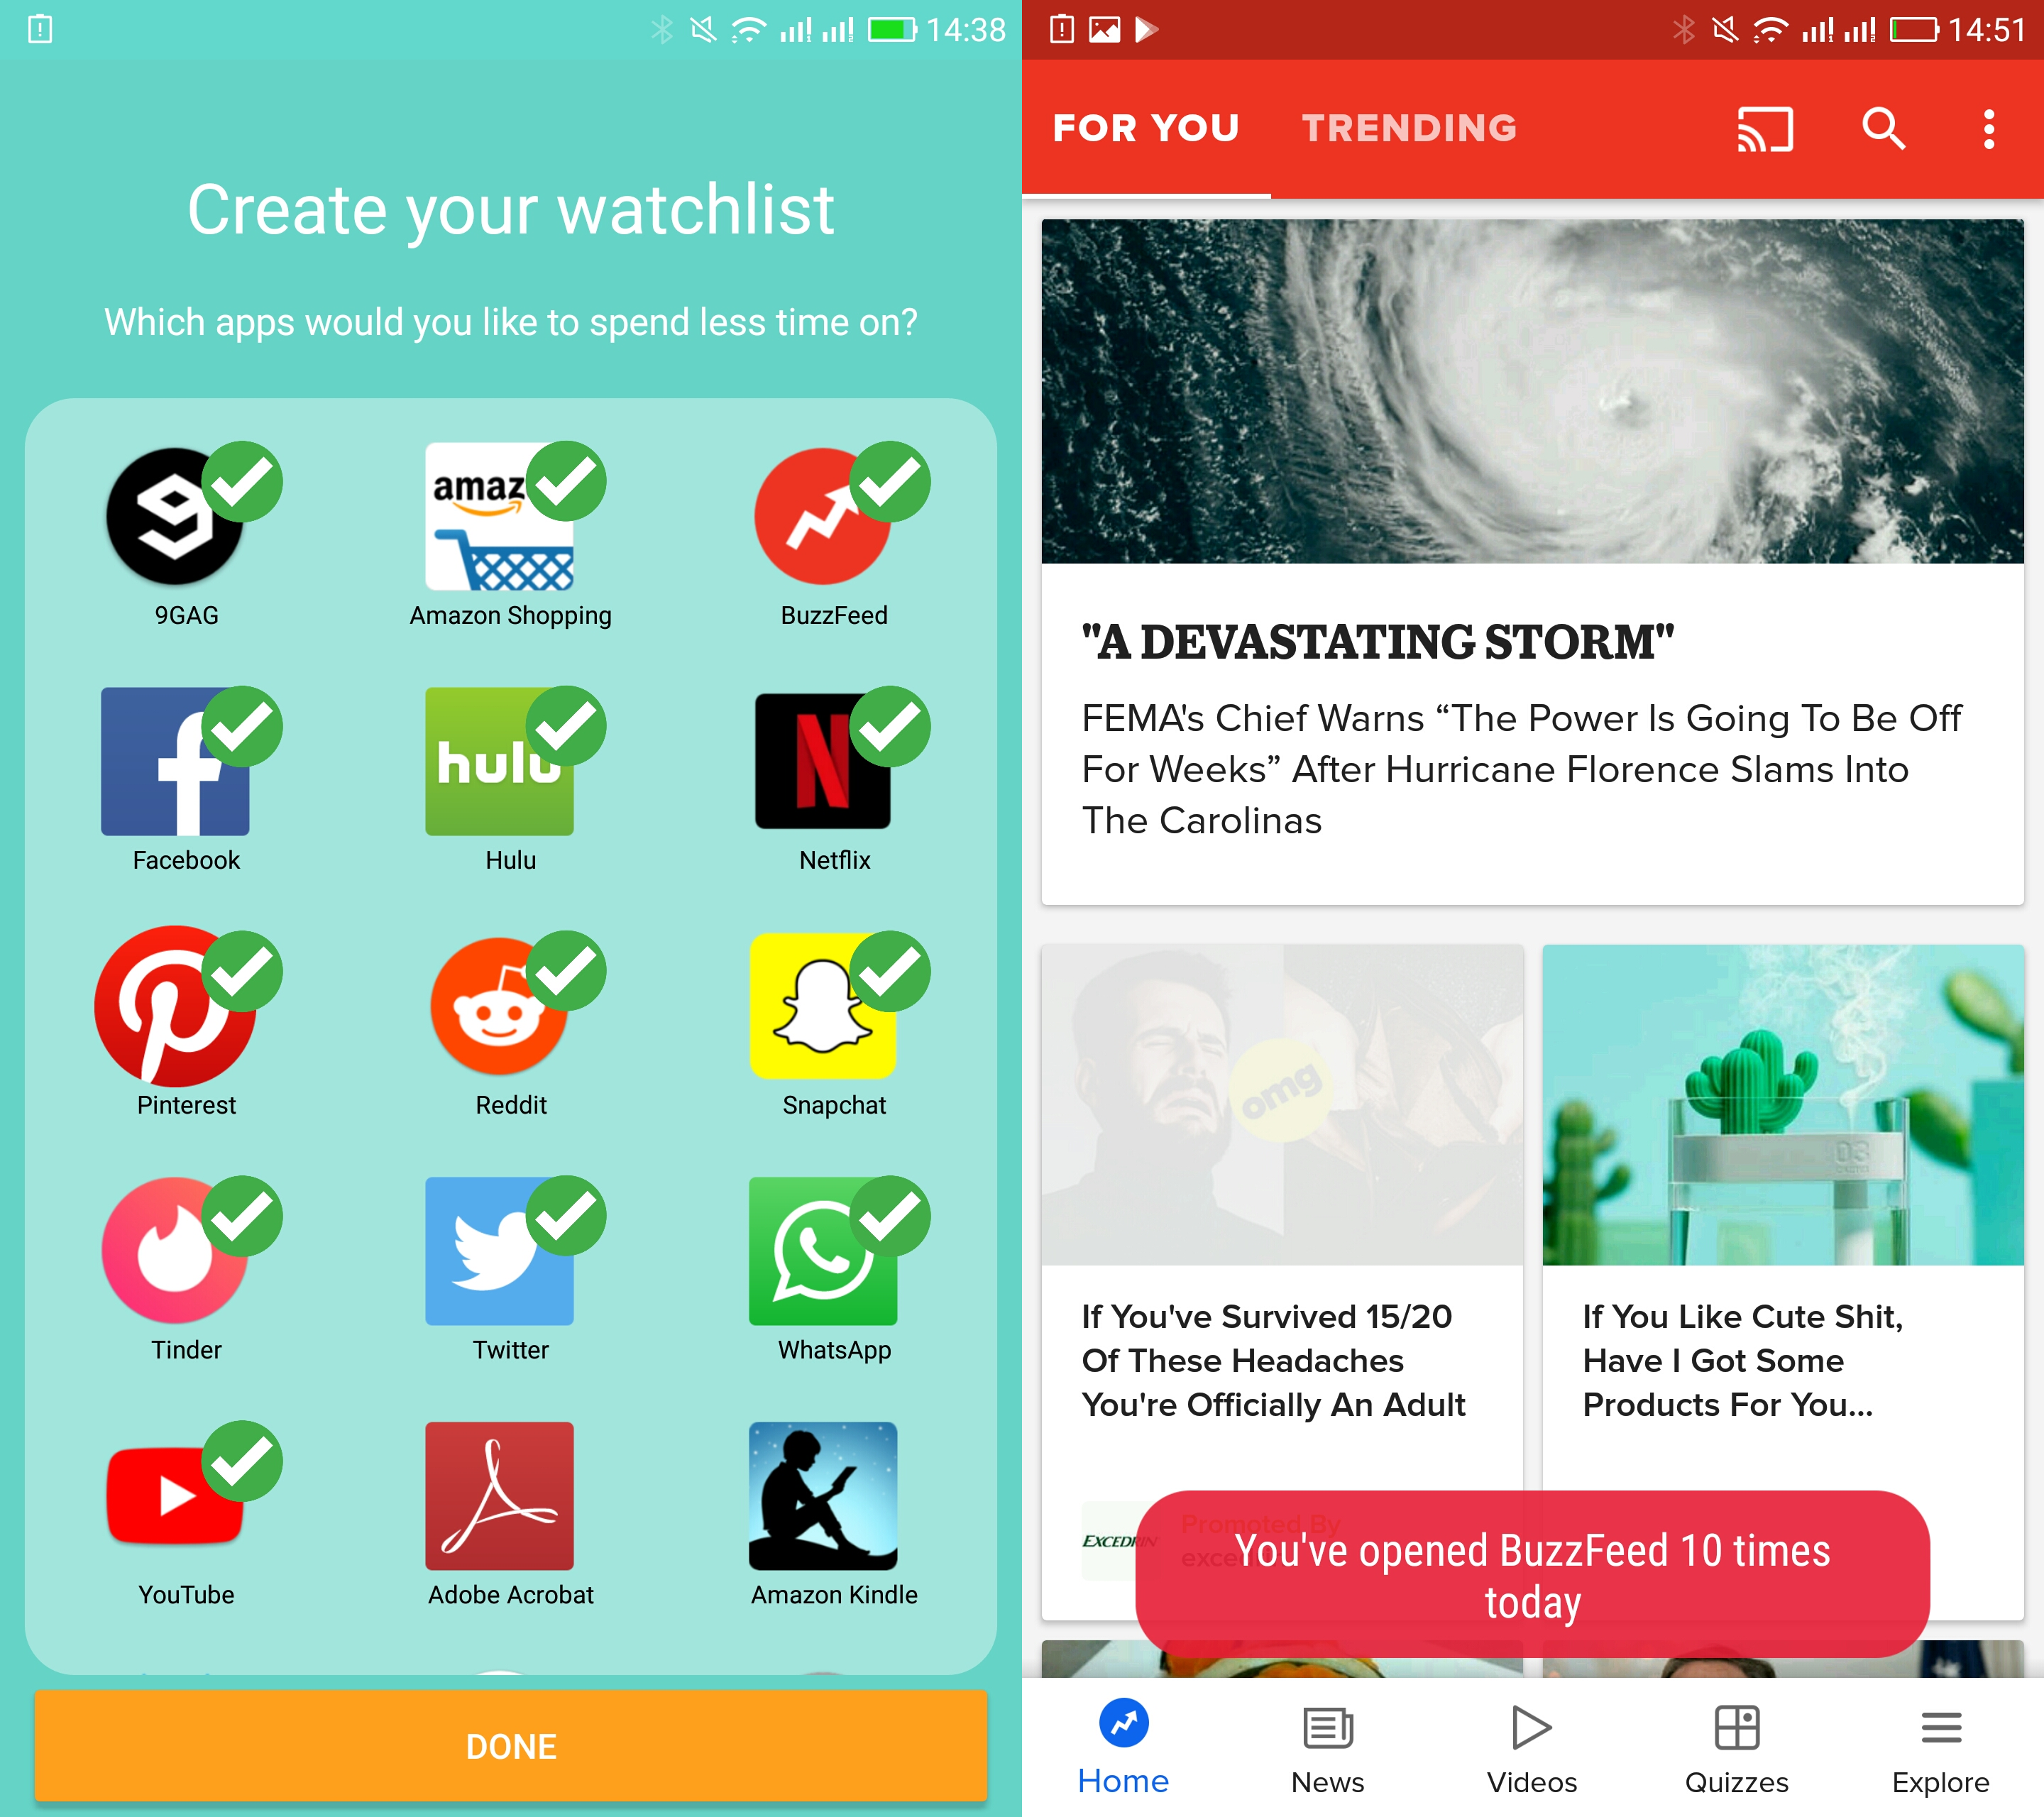
\includegraphics[width=\linewidth]{figures2/android_combined}
\caption{Screenshots from the mobile version of HabitLab.\\
Left: The goal selection screen, where users choose which apps to spend less time on.\\
Right: An example intervention, which shows the visit count when a user opens a goal app. %\msb{save space by cutting the image after the Iqiyi row. No point in having a nearly empty row at the bottom}
}
  \label{fig:android-goal-selection}
\end{figure}

% \begin{figure}[tb]
% \begin{minipage}[t]{0.49\linewidth}
% 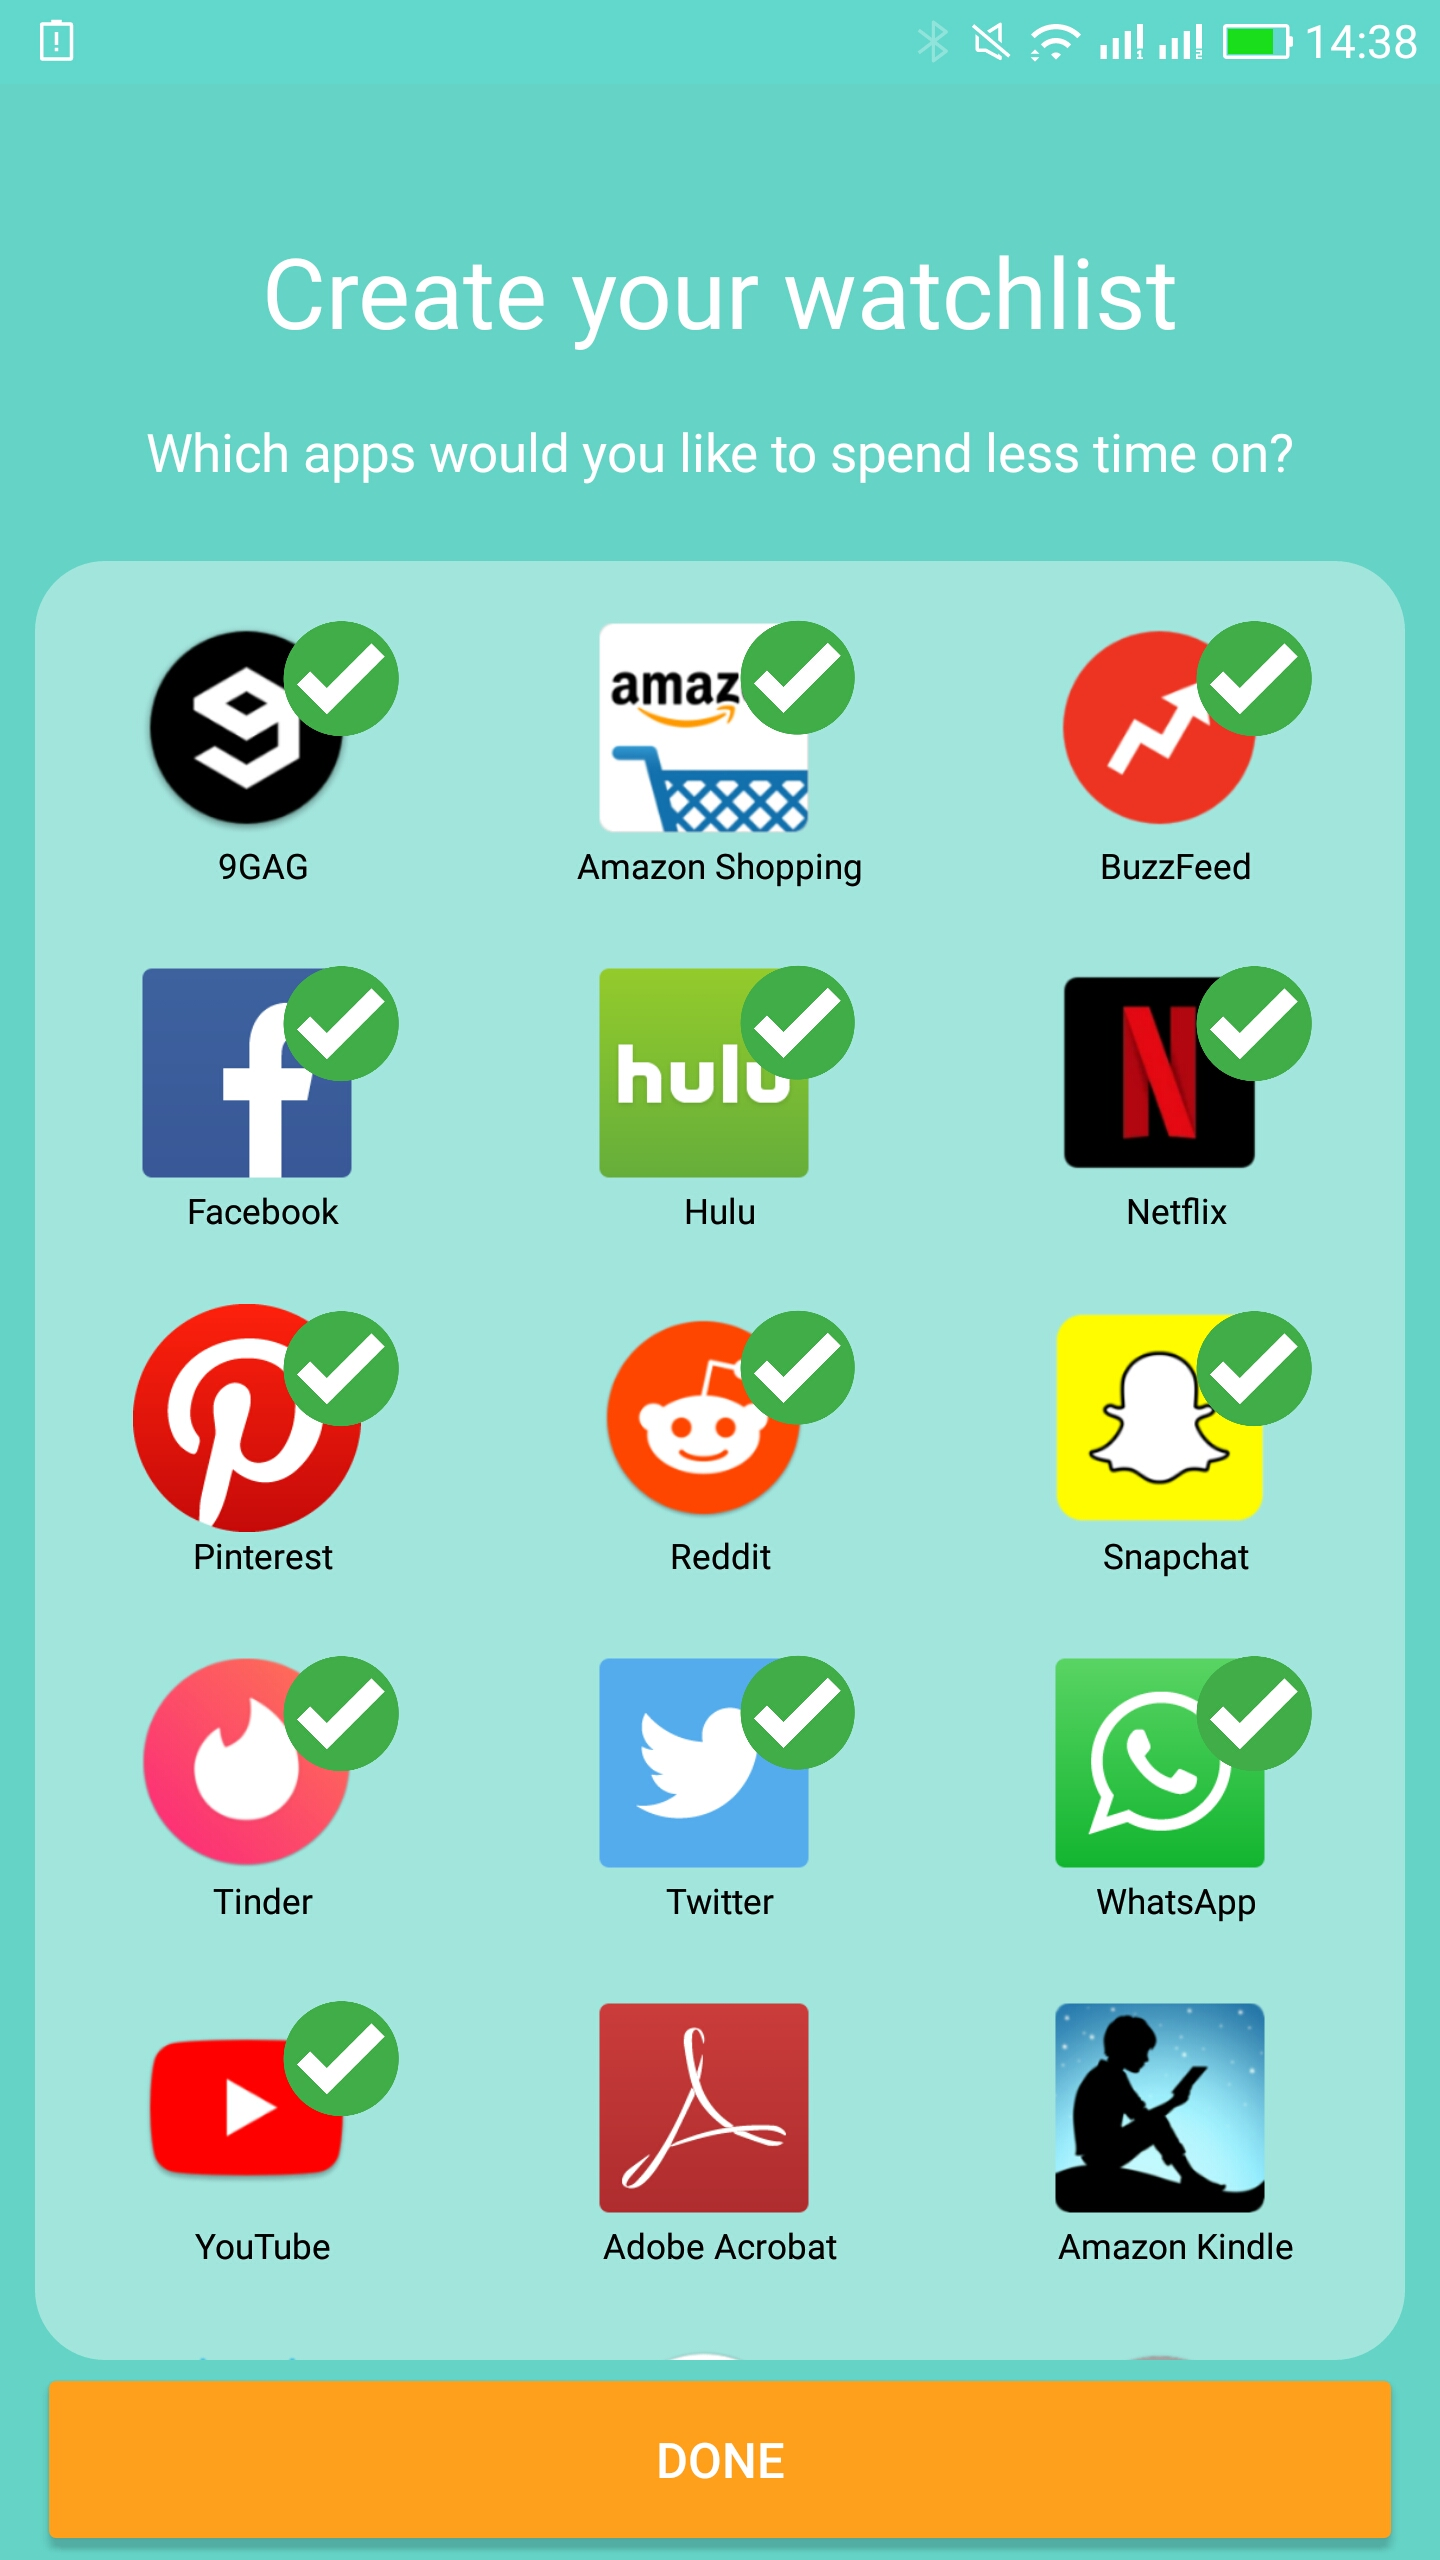
\includegraphics[width=\linewidth]{figures2/android-goal-selection}
% \caption{The goal selection screen, where users choose which apps to spend less time on (mobile version). %\msb{These two mini vertical figures are hard to read. Make it one figure with one caption underneath both.}
% }
%   \label{fig:android-goal-selection}
% \end{minipage}%
% \hfill
% \begin{minipage}[t]{0.49\linewidth}
% 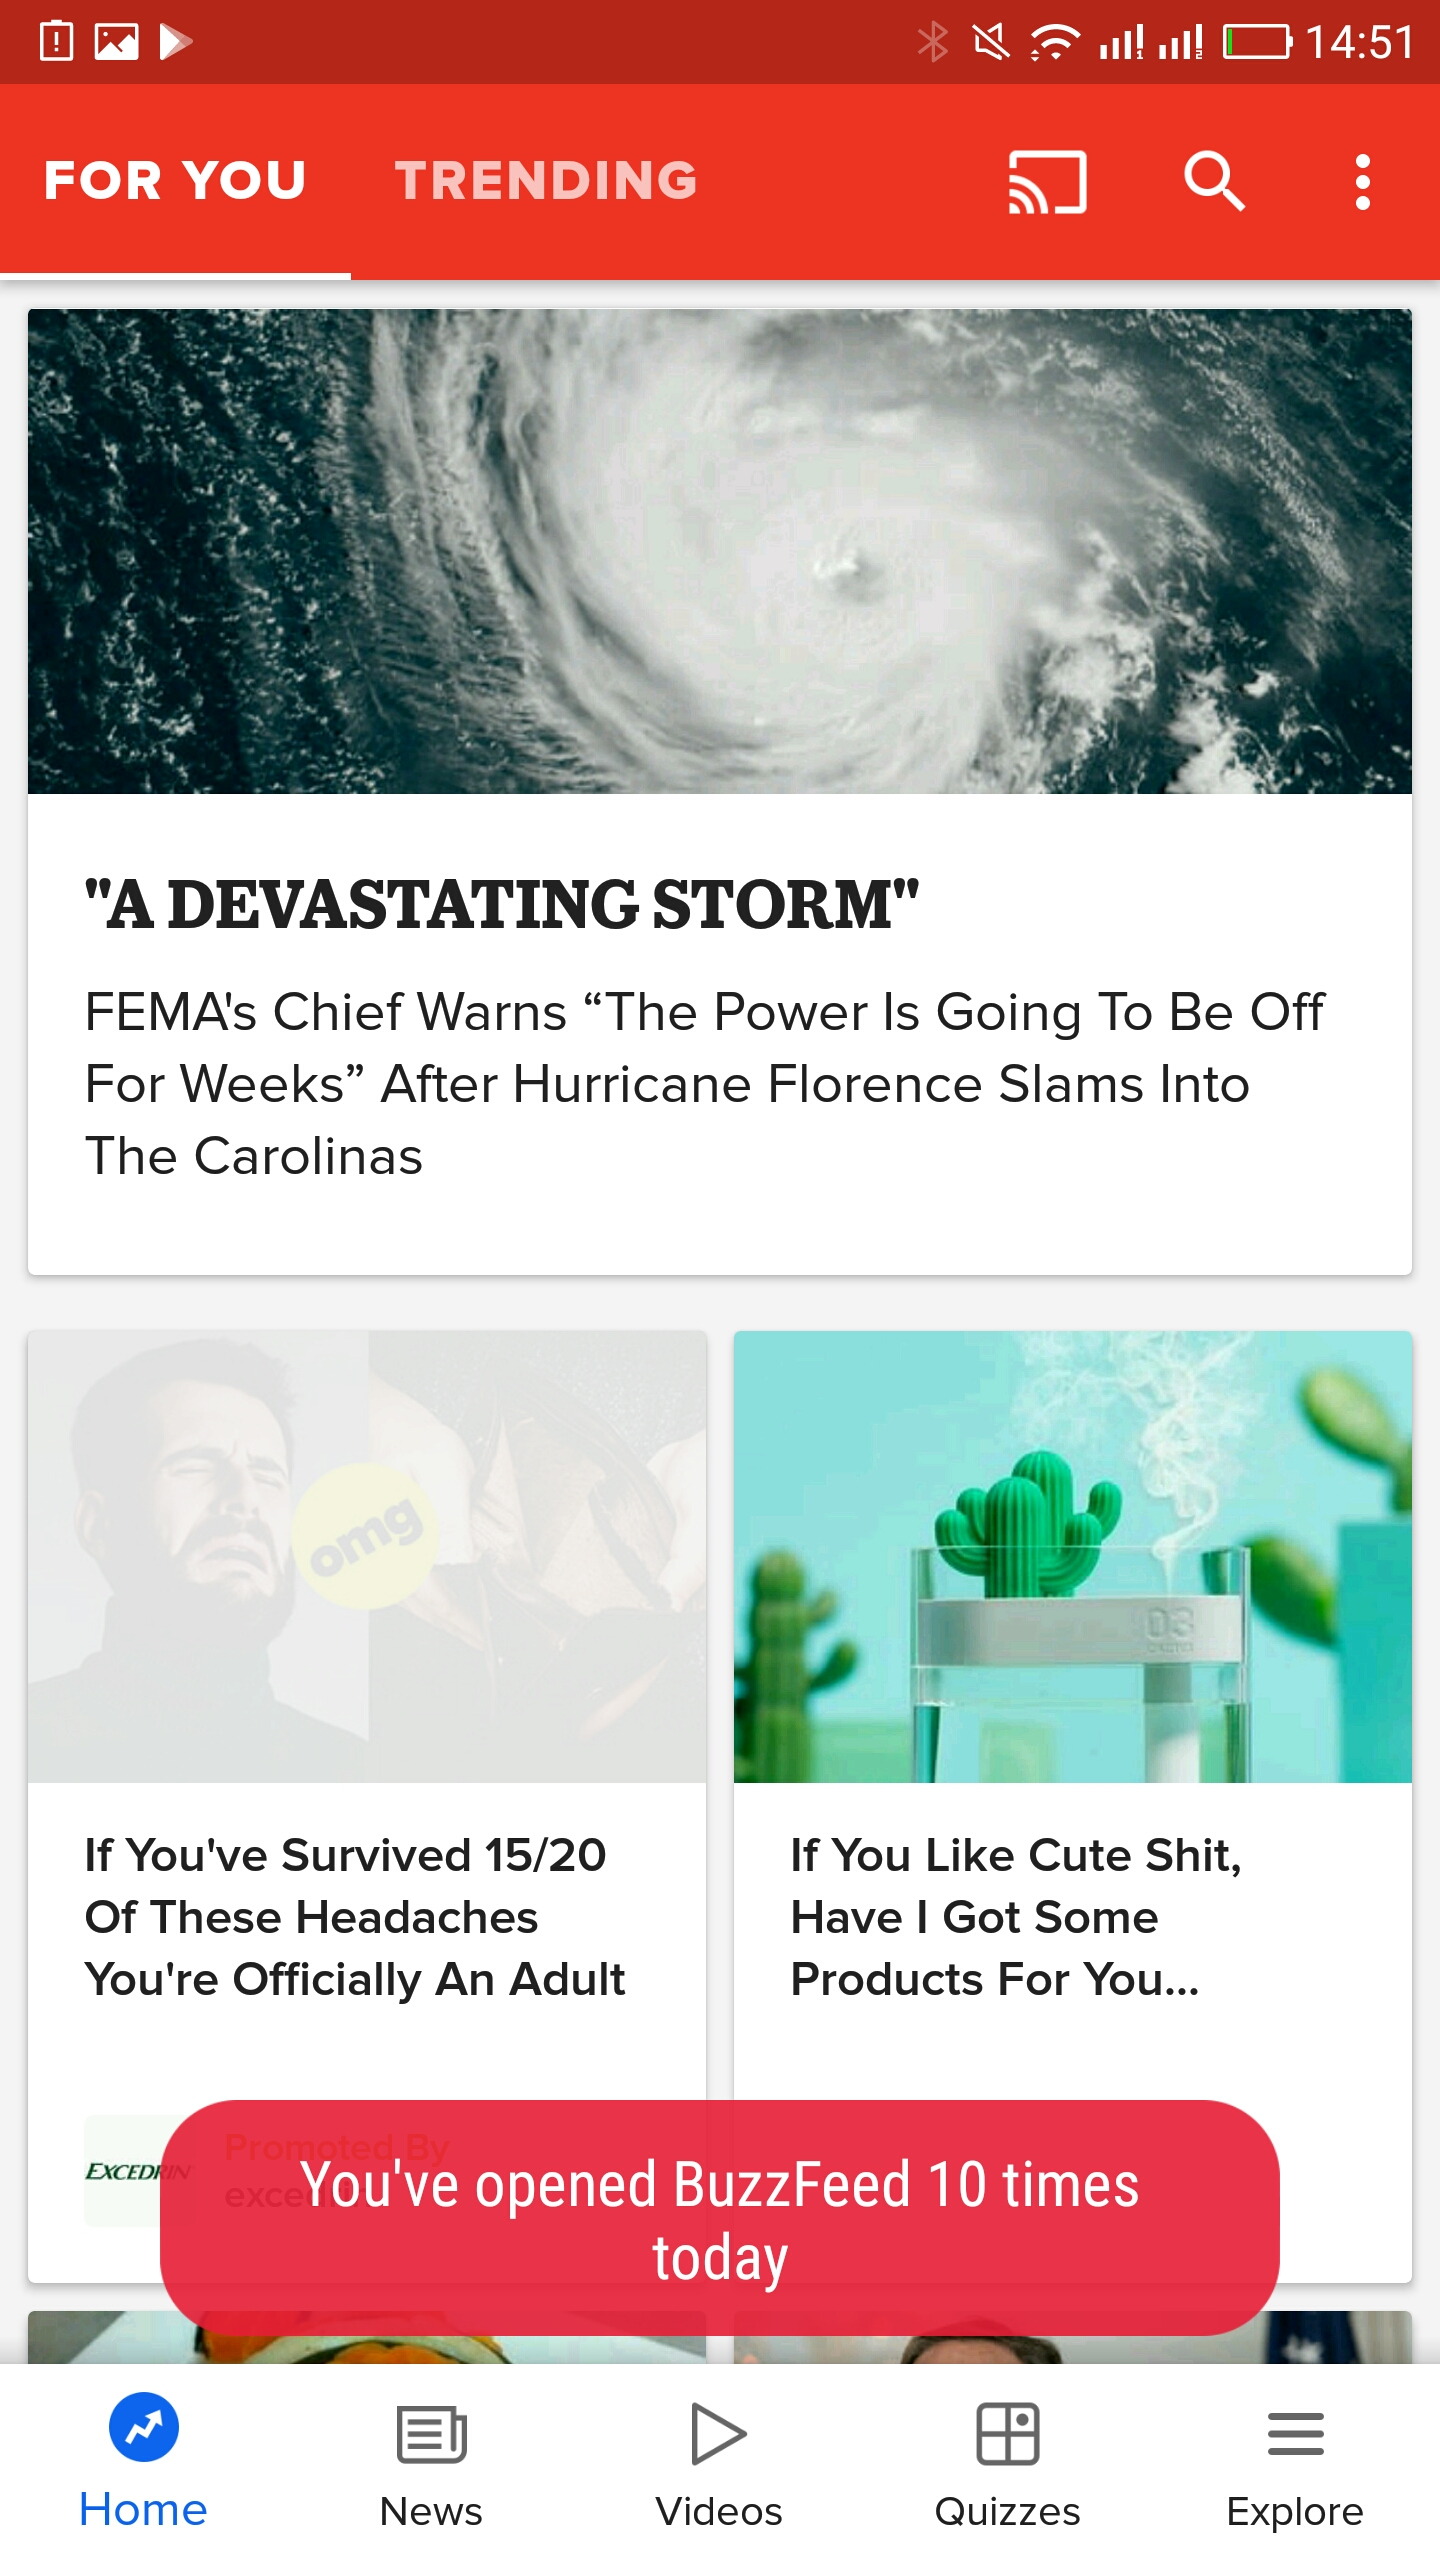
\includegraphics[width=\linewidth]{figures2/android-intervention}
% \caption{An example intervention, which shows the visit count when a user opens an app (mobile version).}
%   \label{fig:android-intervention}
% \end{minipage}
% \end{figure}

% \begin{figure}
% 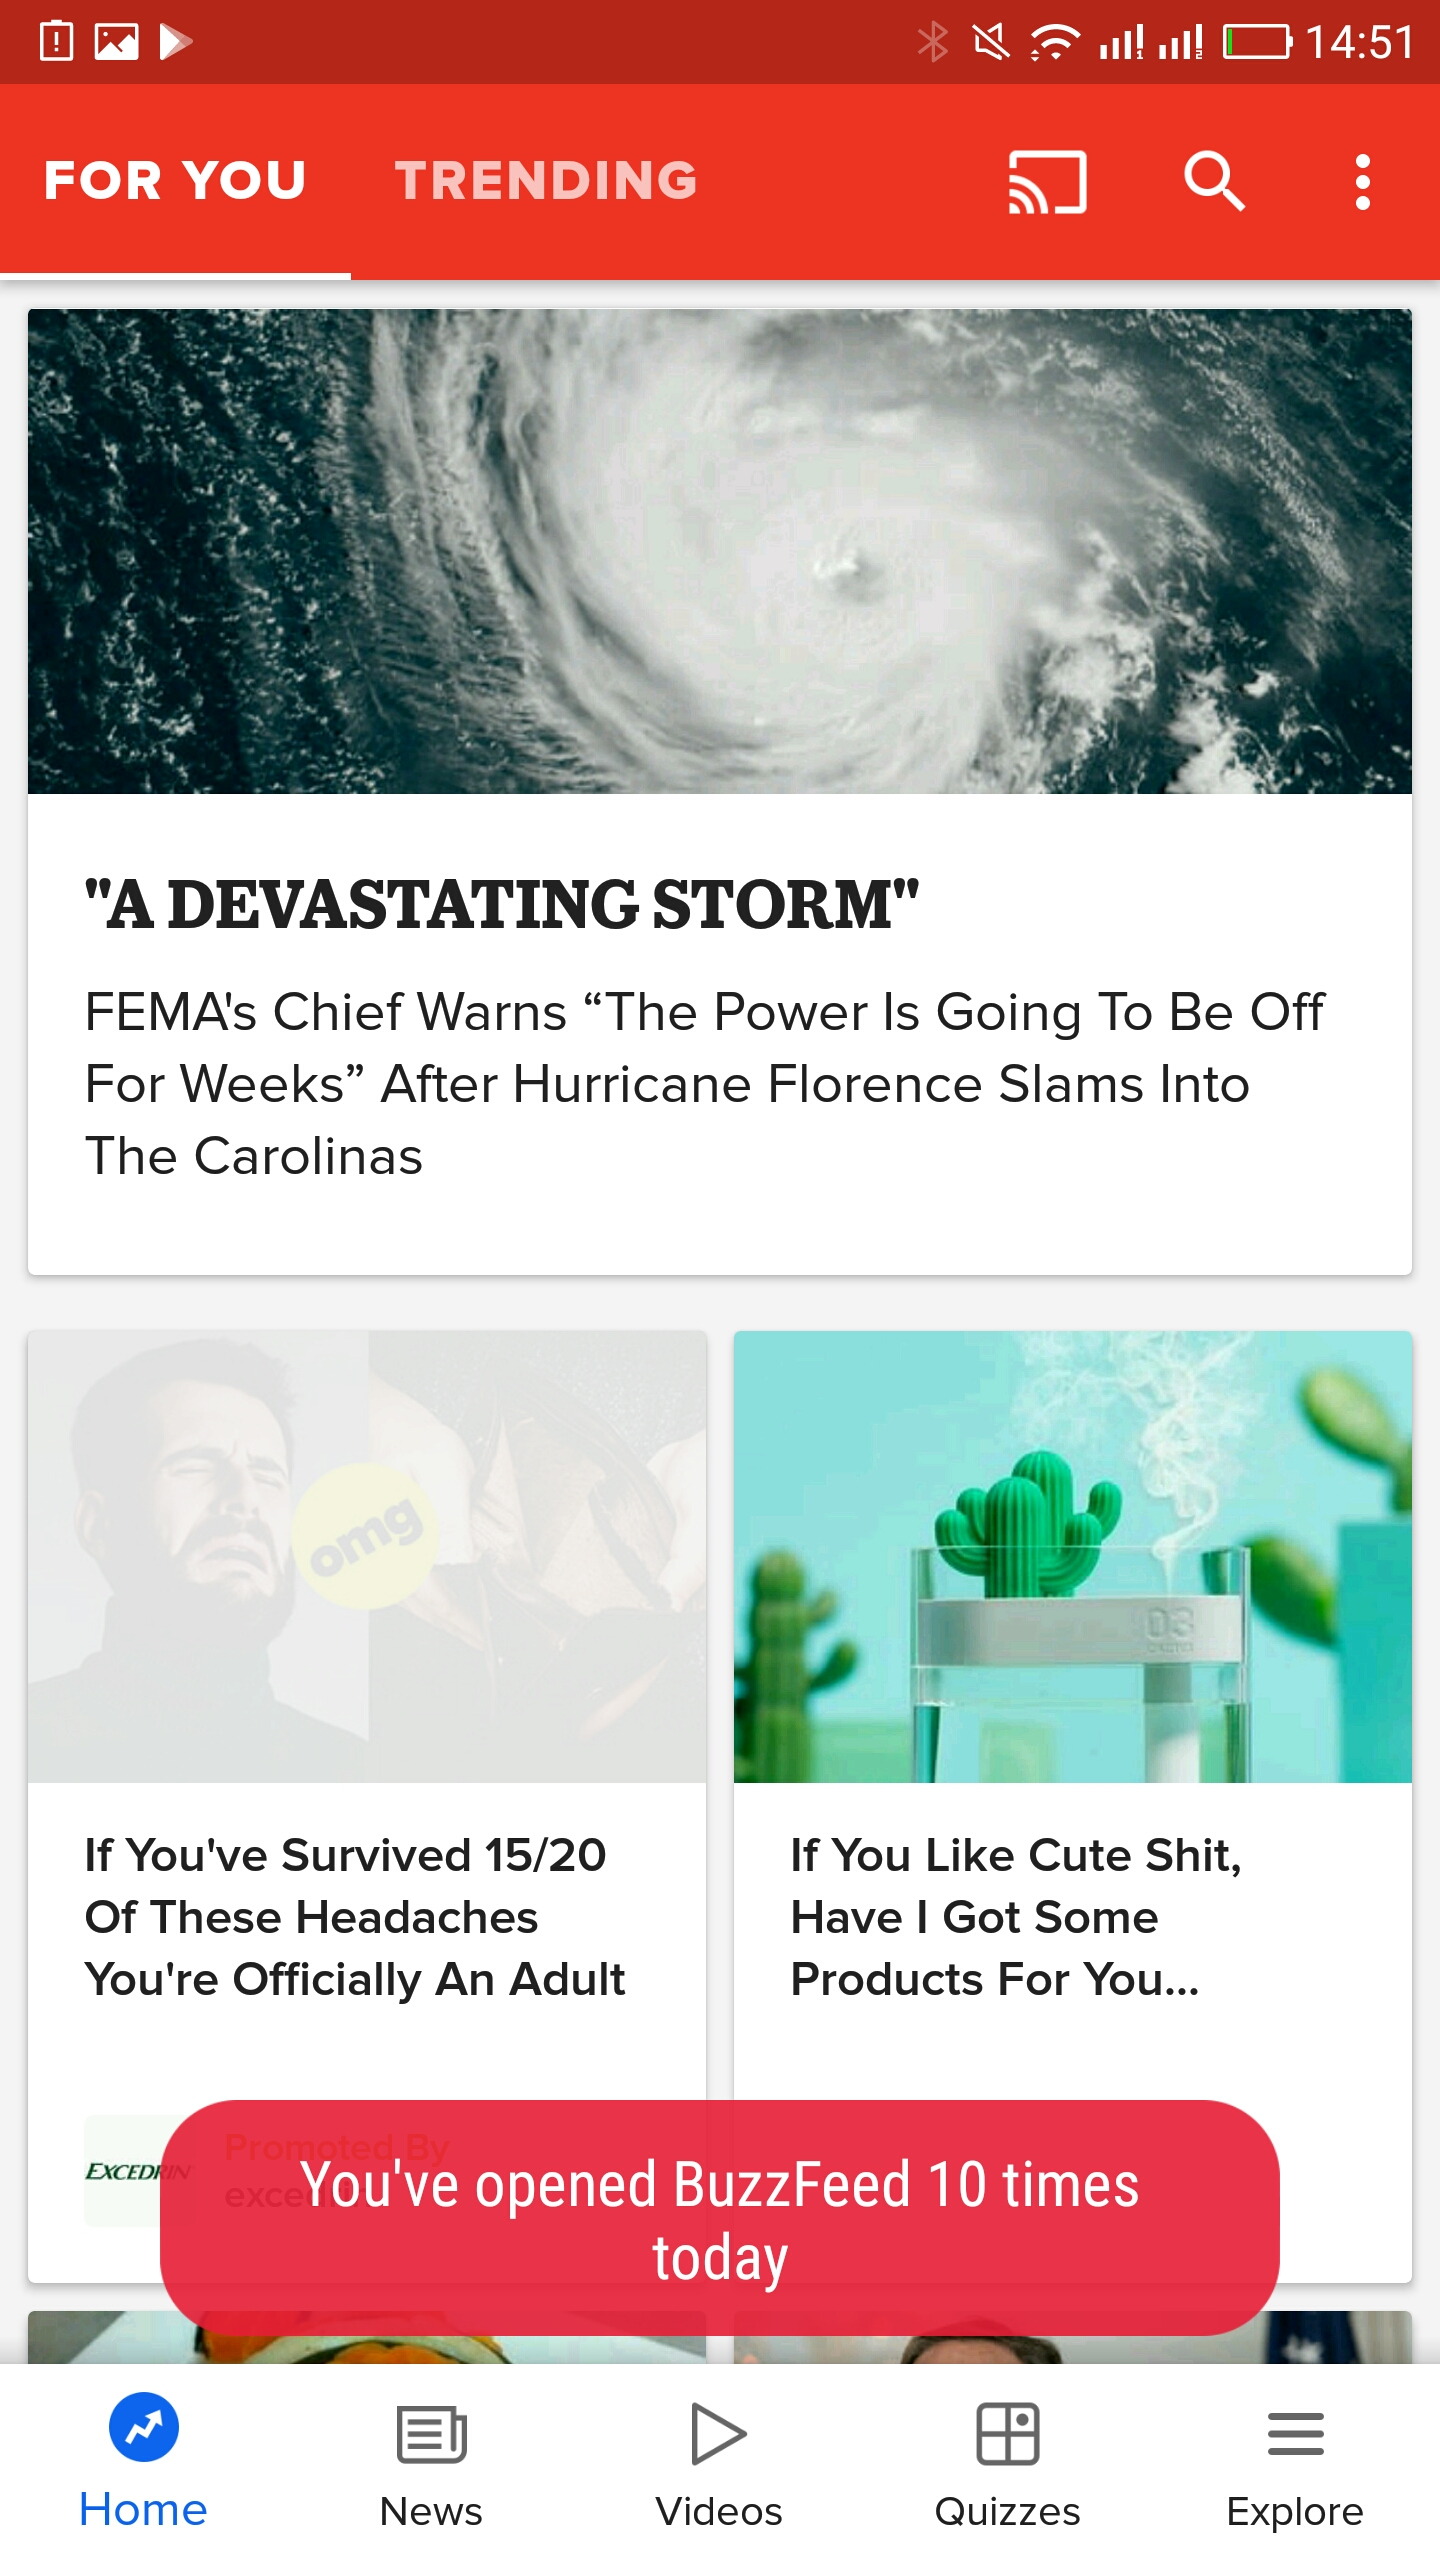
\includegraphics[width=\linewidth]{figures2/android-intervention}
% \caption{Mental model interface: each time the user sees a new intervention, HabitLab names it and explains about rotation.}
%   \label{fig:info}
% \hfill
% \includegraphics[width=\linewidth]{figures2/android-watchlist}
% \caption{User control interface: in addition to the mental model information, HabitLab gives users a direct interface to disable the new intervention.}
%   \label{fig:power}
% \end{figure}

\begin{figure}
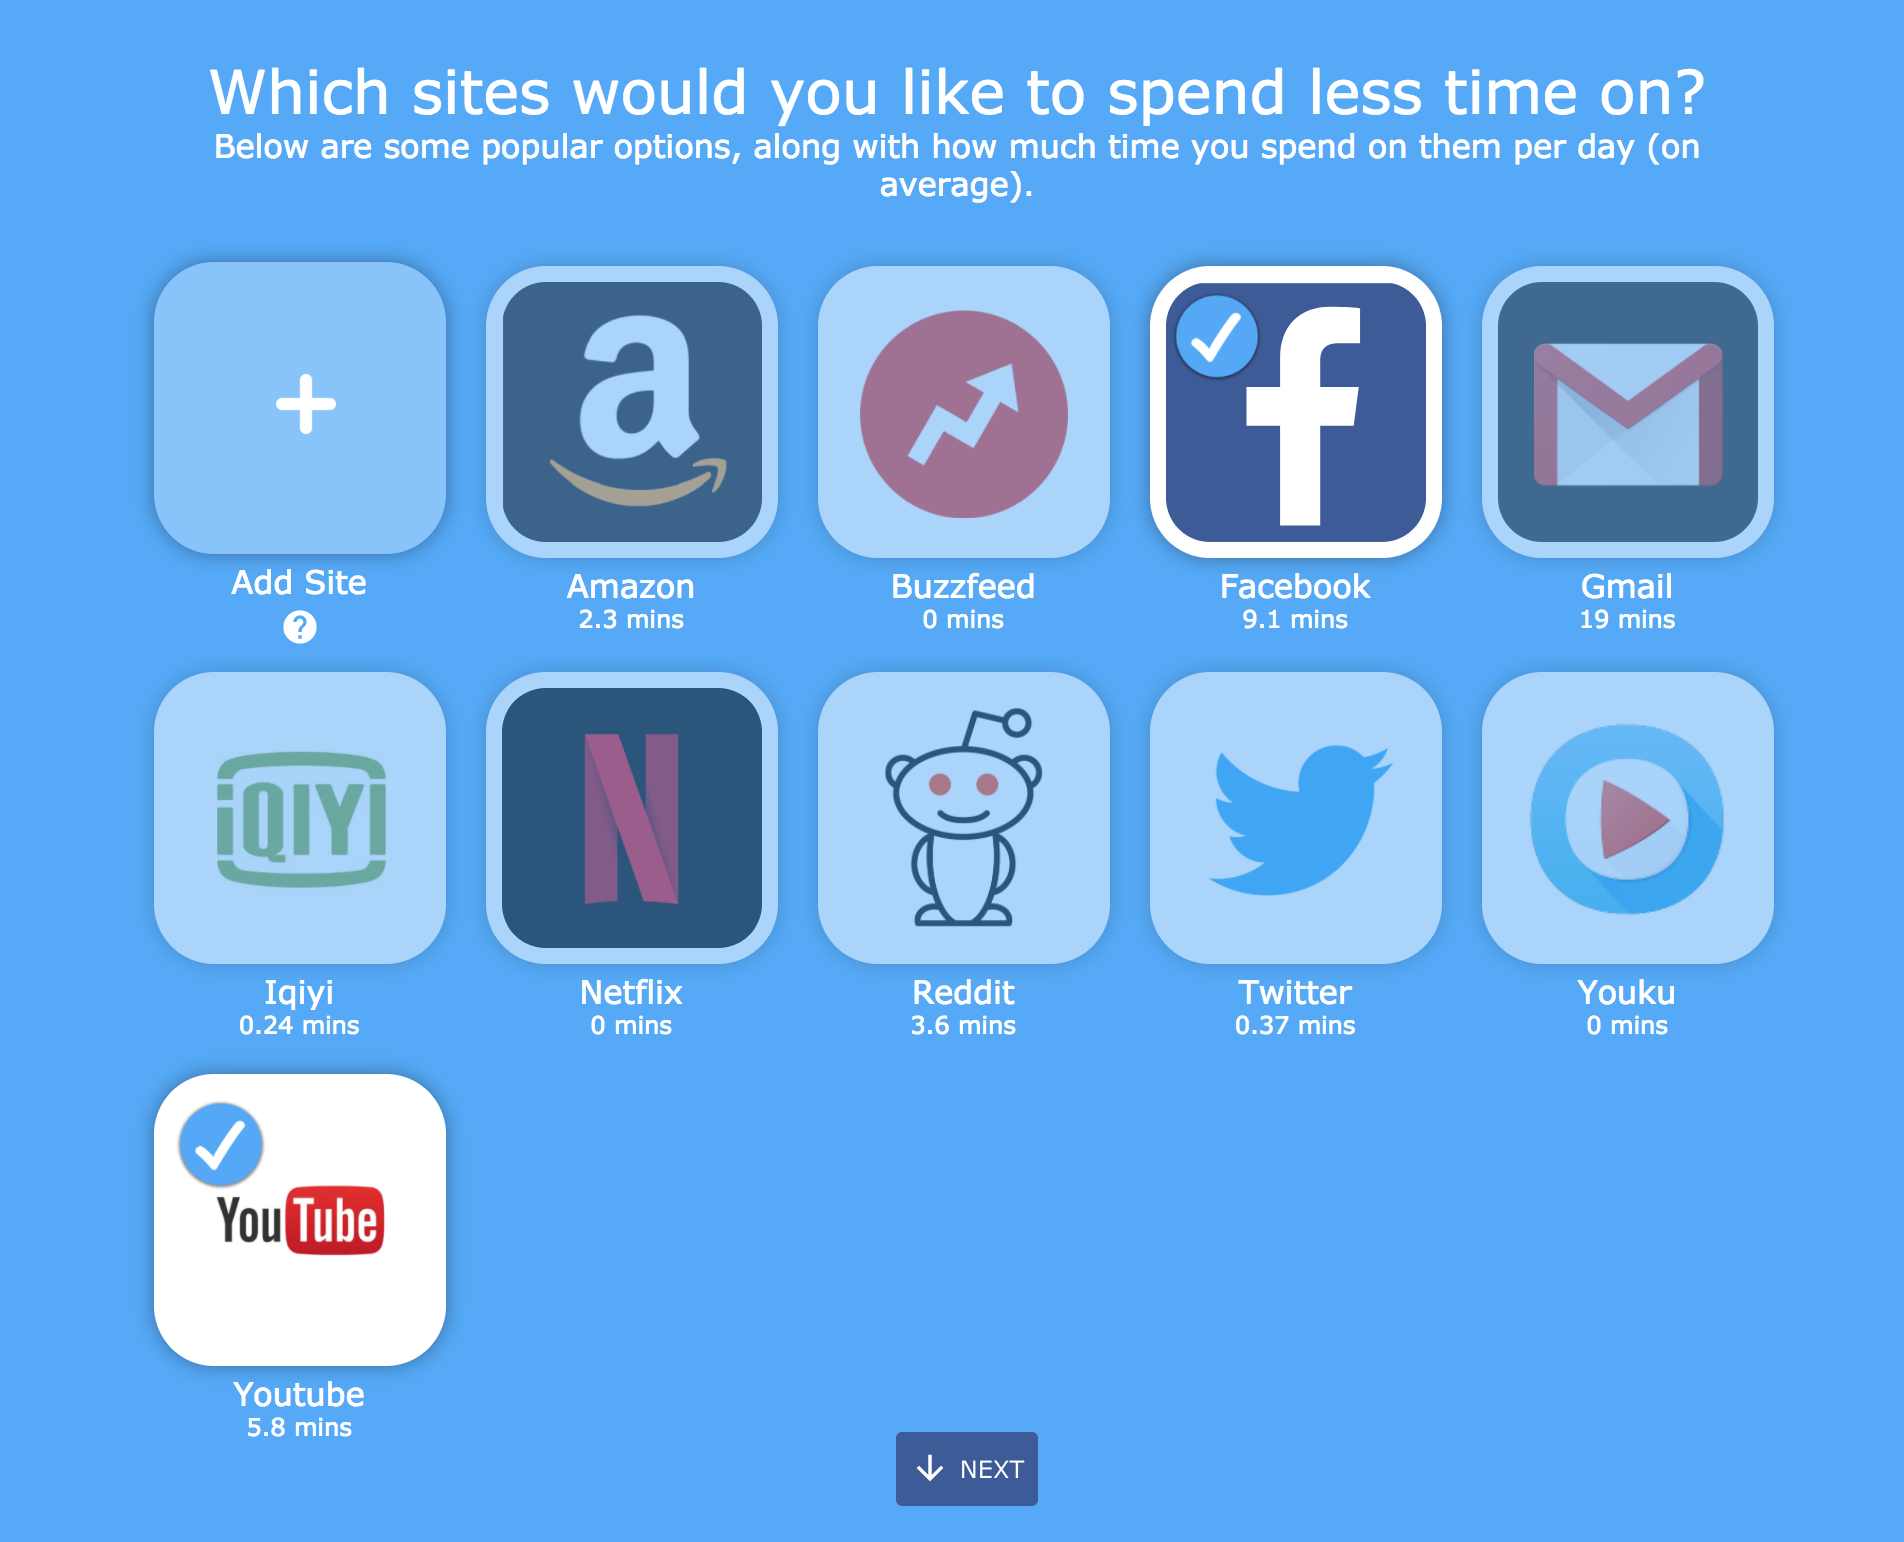
\includegraphics[width=\linewidth]{figures2/chrome-goal-selection}
\caption{The goal selection screen, where users choose which sites to spend less time on (browser version). %\msb{save space by cutting the image after the Iqiyi row. No point in having a nearly empty row at the bottom}
}
  \label{fig:chrome-goal-selection}
\end{figure}

\begin{figure}
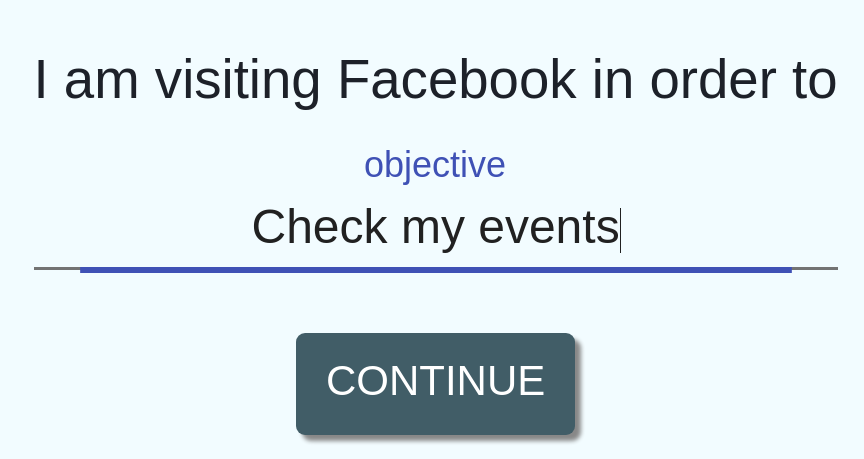
\includegraphics[width=\linewidth]{figures2/chrome-intervention-v3}
\caption{An example intervention, which asks a user to write their objective for visiting a site (browser version). %\msb{This page is really crowded with figures. I suggest moving one onto the next page.} 
% \msb{Save space by reducing this figure to start just above ``I am visiting FB to...''. The turn off button isn't necessary and it adds a ton of space to the paper.}
}
  \label{fig:chrome-intervention}
\end{figure}

Both versions follow the structure of allowing users to choose what they wish to spend less time on (setting goals), and deploying interventions to meet those goals. %The format of the goals differ between the two platforms.
On the Chrome version, users choose sites to spend less time on (goal sites -- for example, \url{facebook.com}), as shown in Figure~\ref{fig:chrome-goal-selection}. On Android, users choose particular apps to spend less time on (goal apps -- for example, the Facebook Android app), as shown in Figure~\ref{fig:android-goal-selection}. Interventions are deployed when users visit a goal site on Chrome (Figure~\ref{fig:chrome-intervention}), and when users open a goal app on Android, as shown in Figure~\ref{fig:android-goal-selection}.

\begin{figure}[b]
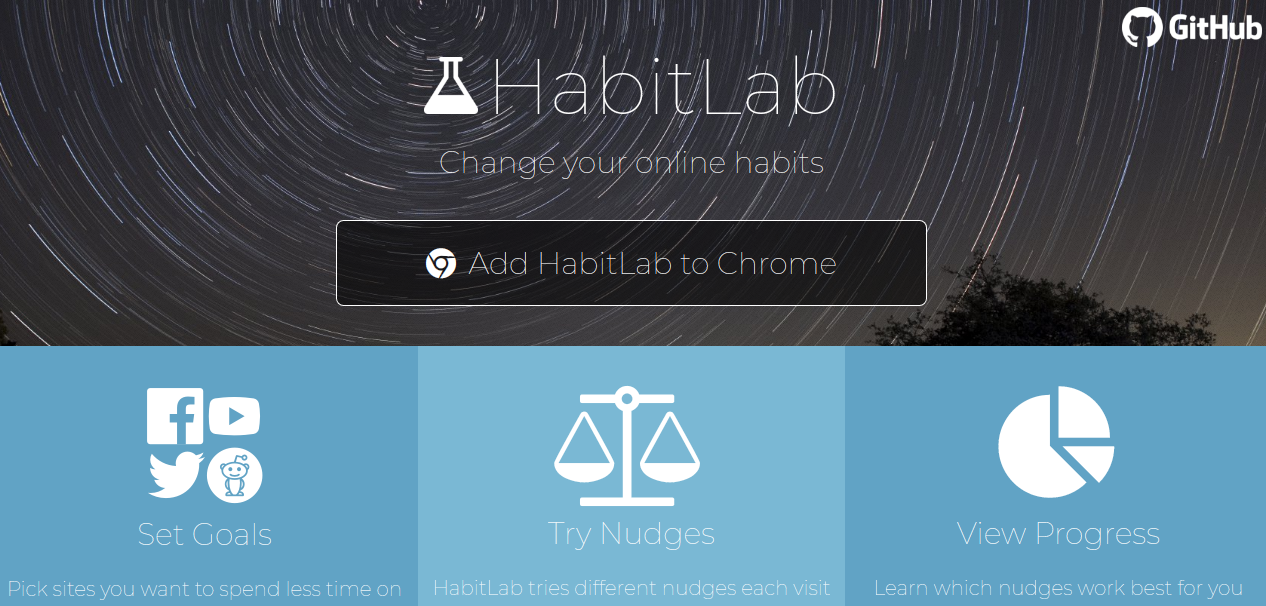
\includegraphics[width=\linewidth]{figures/homepage_cropped}
\caption{HabitLab's homepage describes the browser extension and mobile application. Users adopt it to try out a large number of different possible interventions, called nudges.}
\label{fig:homepage}
\end{figure}

%\section{Browser Version}

Users install the extension, and go through an onboarding process where they select sites and apps they wish to reduce their time on (Figure~\ref{fig:onboarding_sites}). There are predefined options---Facebook and YouTube are selected by default, as they were the most commonly used---but users can also add any custom site. Custom sites are suggested via an analysis of the user's browsing history. The system explains to users that they will be shown a variety of interventions (Figure~\ref{fig:onboarding_nudges}), a form of self-experimentation~\cite{Karkar:2017:TFS:3025453.3025480}, to help them reduce time on that site. These interventions are typically targeted to each site, for example a news feed blocker for Facebook or a related video hider for YouTube. However, some interventions such as a stopwatch timer can be added to any custom site. Users can preview the interventions for the sites they select, and enable or disable each intervention if desired. Users can later enable or disable interventions and sites through a settings page.

\begin{figure}
\begin{minipage}[t]{0.49\linewidth}
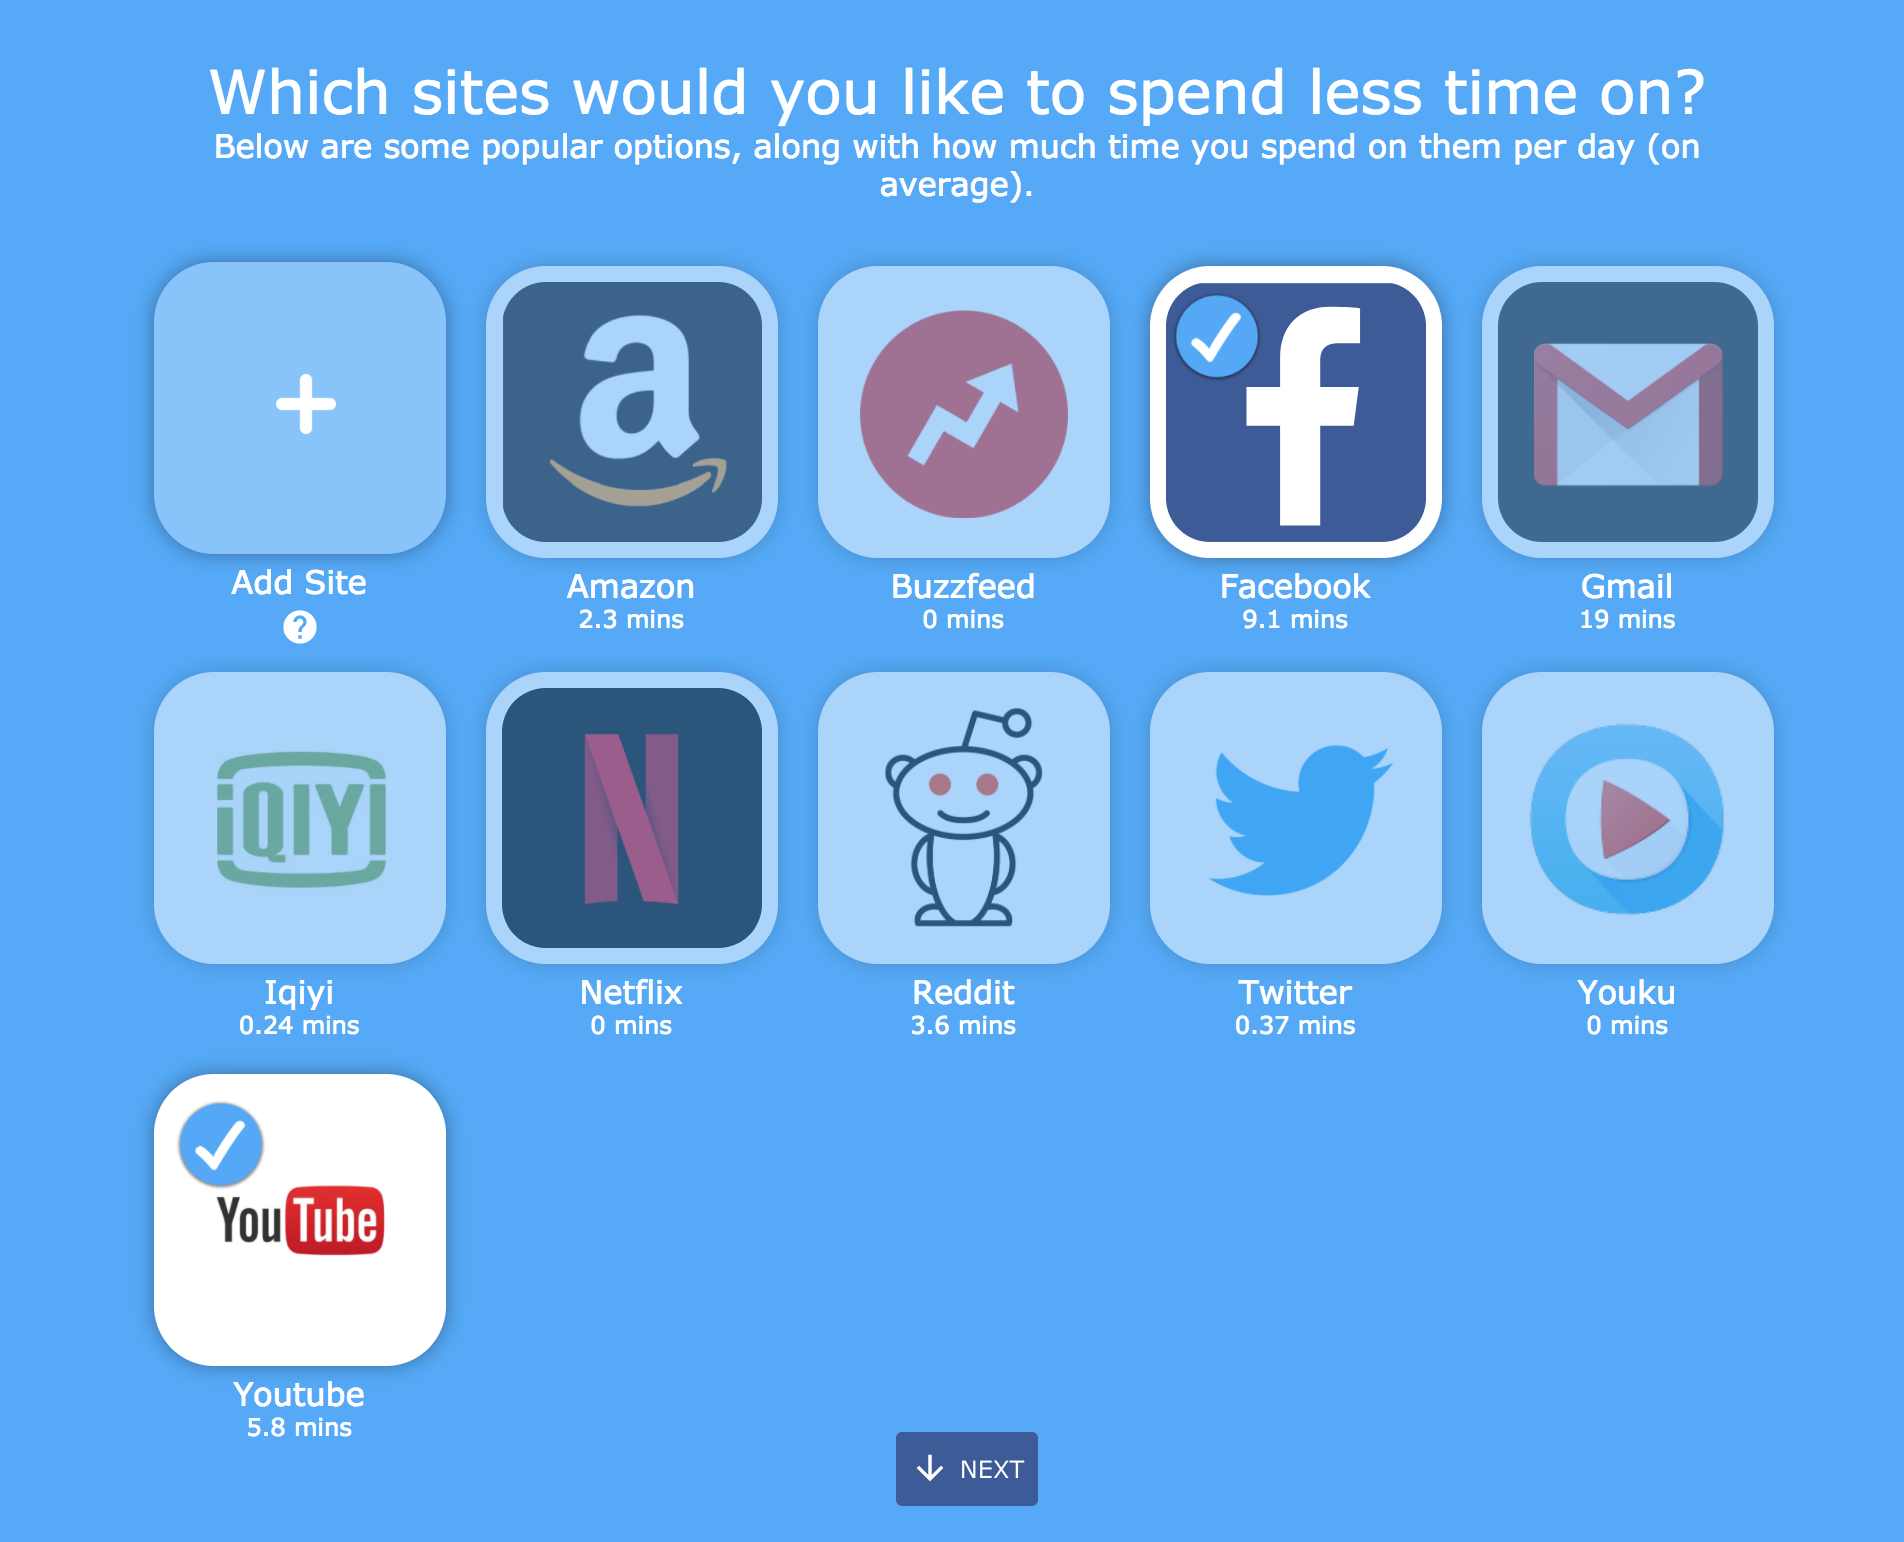
\includegraphics[width=\linewidth]{figures/onboarding_sites}
\caption{During onboarding, users choose which sites they want to spend less time on.}
  \label{fig:onboarding_sites}
\end{minipage}
\hfill
\begin{minipage}[t]{0.49\linewidth}
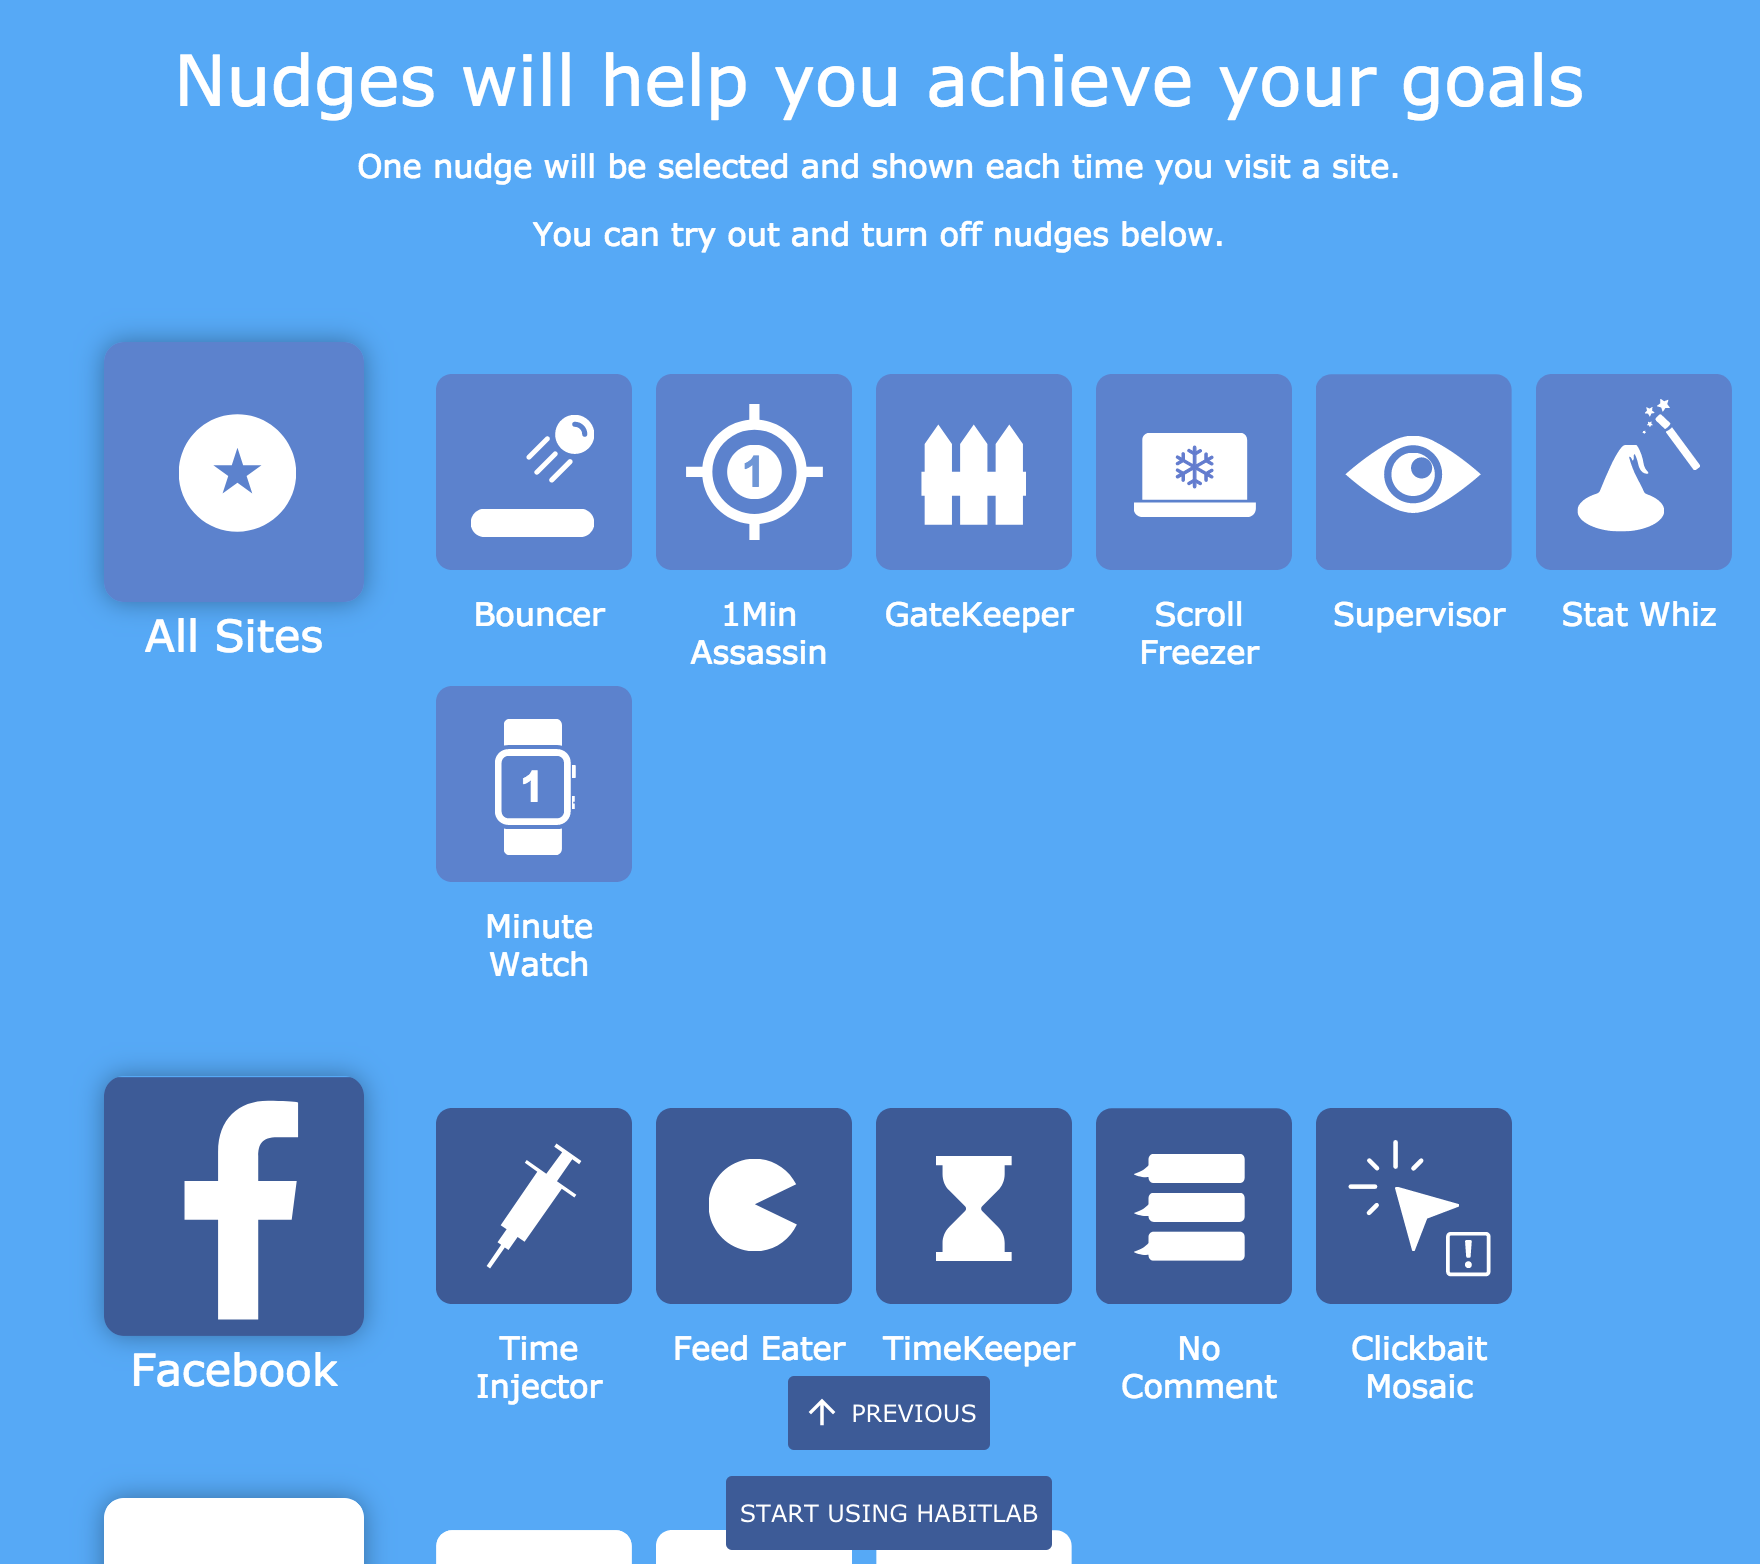
\includegraphics[width=\linewidth]{figures/onboarding_nudges_short}
\caption{Users are presented with the interventions they will see on each site.}
  \label{fig:onboarding_nudges}
\end{minipage}%
\end{figure}

HabitLab emphasizes to users the availability of multiple interventions and that it may show users different interventions each time they load a page. This emphasis is made clear on the HabitLab website, Chrome store listing, and through features in the dashboard such as visualizing the relative effectiveness of different interventions. HabitLab implements a multi-armed bandit algorithm to explore and find the interventions that are most effective for each user, optimizing for minimizing time spent on a site. However, in the experiments in this paper, we disabled this functionality and instead used simple random selection so that we can study the effects of rotation in isolation.

\section{Mobile and Browser Versions}

The Chrome extension and Android app differ in some minor details. They support different sets of goals: users select apps to reduce time on in the Android version, whereas users choose sites to reduce time on in the Chrome version. Additionally, the specific set of interventions available differs between the platforms to fit the design languages of the browser and the mobile phone. The Chrome version has certain interventions which are site-specific -- such as a news feed remover that is specific to Facebook. However, because Android does not allow applications to edit each other's view trees, the Android version's interventions are all glass pane overlays, and thus are general and can be used on any app. The concept of a session is different on the platforms: in the Chrome version, a session is time on a site until that tab is either closed or the user goes to a different domain. Time measured is active time -- so if the tab is not focused, or if there is no keyboard or mouse activity for over a minute, the timer is temporarily paused. However, on Android, because there is no concept of a tab, the measurement of a session is different. There, a session is considered the duration over which an app is opened and focused. Closing the app, switching to a different app, or turning off the phone will end the current session.

\section{Design of HabitLab Interventions}

HabitLab can track time and deploy interventions on all sites, but some interventions are tailored towards specific sites. There are 27 interventions total: seven generic interventions that can be used on all sites, five interventions designed specifically for Facebook, and additional ones designed specifically for YouTube, Reddit, Twitter, Netflix, Gmail, Amazon, iQiyi, and Youku.

Interventions are designed drawing on theories of behavior change---for example, goal setting theory~\cite{locke2002building}, persuasion~\cite{cialdini1987influence,fogg2002persuasive,abraham2008taxonomy}, and gamification~\cite{deterding2011game}. A sample of the interventions available for Facebook, categorized according to underlying strategies and theories, are shown in Table~\ref{tab:theories}. Screenshots of some Facebook interventions are shown in Figure~\ref{fig:interventions}.  Descriptions of the interventions on the Chrome and Android versions can be found at the end of this chapter. %\msb{always use non breaking space \~ between Figure and number, and between sentence and citation block}
% , and health ~\cite{abraham2008taxonomy} \msb{health is not a theory of behavior change}

%The design of HabitLab's interventions is based on theories such as Cialdini's factors of influence~\cite{cialdini1987influence} and the behavior change wheel taxonomy of behavior change interventions~\cite{abraham2008taxonomy}. Description of the interventions on the Chrome and Android versions can be found in the Appendix.

Not all interventions are enabled by default---this is because some of them have higher attrition rates than others. Non-default interventions can be previewed and enabled by users during onboarding and on the settings page. The interventions enabled by default were the ones we found to have low attrition rates during pilot deployments---we chose this strategy to ensure user retention and growth, which is a prerequisite for gathering data in an in-the-wild experiment setting.

\begin{table}[tb]
\small
\begin{center}
\begin{tabular}{ p{3.3cm} p{3.4cm} p{6.2cm} }
  \textbf{Strategy} & \textbf{Theory} & \textbf{Intervention} \\
  %\hline
  Commitment & Self-consistency theory~\cite{allgeier1979waffle,cialdini1987influence,sherman1980self} & Ask the user to set a goal for the length of time they will stay on the site (generic) \\
  Enforce default limits & Status quo bias ~\cite{samuelson1988status} & Automatically close tab after 60 seconds unless the user clicks a button to ask for more time (generic) \\
%  Enforce default limits & Status quo bias ~\cite{samuelson1988status} & Prevents scrolling unless the user clicks a button to continue scrolling (generic) \\
Reduce social incentives & Social proof~\cite{sherif1935study,cialdini1987influence} & Hide Facebook comments by default (default) \\
  Delaying Rewards & Operant conditioning~\cite{baron1991analyzing} & Make the user wait 10 seconds before visiting Facebook (generic) \\
%  Delaying Rewards & Operant conditioning~\cite{baron1991analyzing} & Shows a page with time spent on Facebook today which they need to click through to get to Facebook (generic) \\
Removing Rewards & Operant conditioning~\cite{baron1991analyzing} & Hide the news feed (default) \\
%  Removing Rewards & Operant conditioning~\cite{baron1991analyzing} & Hide videos and clickbait in the news feed \\
% Gamification & Goal setting theory~\cite{locke2002building}, Flow~\cite{csikszentmihalyi1996flow} & Get points and badges for seeing fewer newsfeed items  \\
  Inform the user & Theory of reasoned action~\cite{ajzen1977attitude} & Show a counter at the top of the page of how long user has been on Facebook today (default, generic) \\
%  Inform the user & Theory of reasoned action~\cite{ajzen1977attitude} & Show a toast notification each minute displaying how long they've been on Facebook today (default, generic) \\
%  Inform the user & Theory of reasoned action~\cite{ajzen1977attitude} & Show a desktop notification each minute displaying how long they've been on Facebook today (generic) \\
% Inform the user & Theory of reasoned action~\cite{ajzen1977attitude} & Inject messages into the news feed showing how long they've been on Facebook today (default) \\
  %Make a plan & Theory of planned behavior \cite{gollwitzer1999implementation} & Ask the user to write out a concrete plan for how they will avoid coming back to the site next time they are tempted to do so \\
  % Rewards/punishment & Operant conditioning~\cite{baron1991analyzing} & Block the site for four hours if the user spends too much time on site in this session \\
  %Stress management & Stress coping~\cite{thoits1995stress} & Reflection on stressors that lead to visiting Facebook \\
  
\end{tabular}
\end{center}
%\vspace{-.7em}
\caption{A subset of the interventions for Facebook, categorized according to persuasion strategy and theory. Interventions that are enabled by default are marked \textit{default}, interventions that are available for all sites are marked \textit{generic}.}
\label{tab:theories}
\end{table}


% todo need to retake these screenshots so they're anonymous
\begin{figure}
\centering
	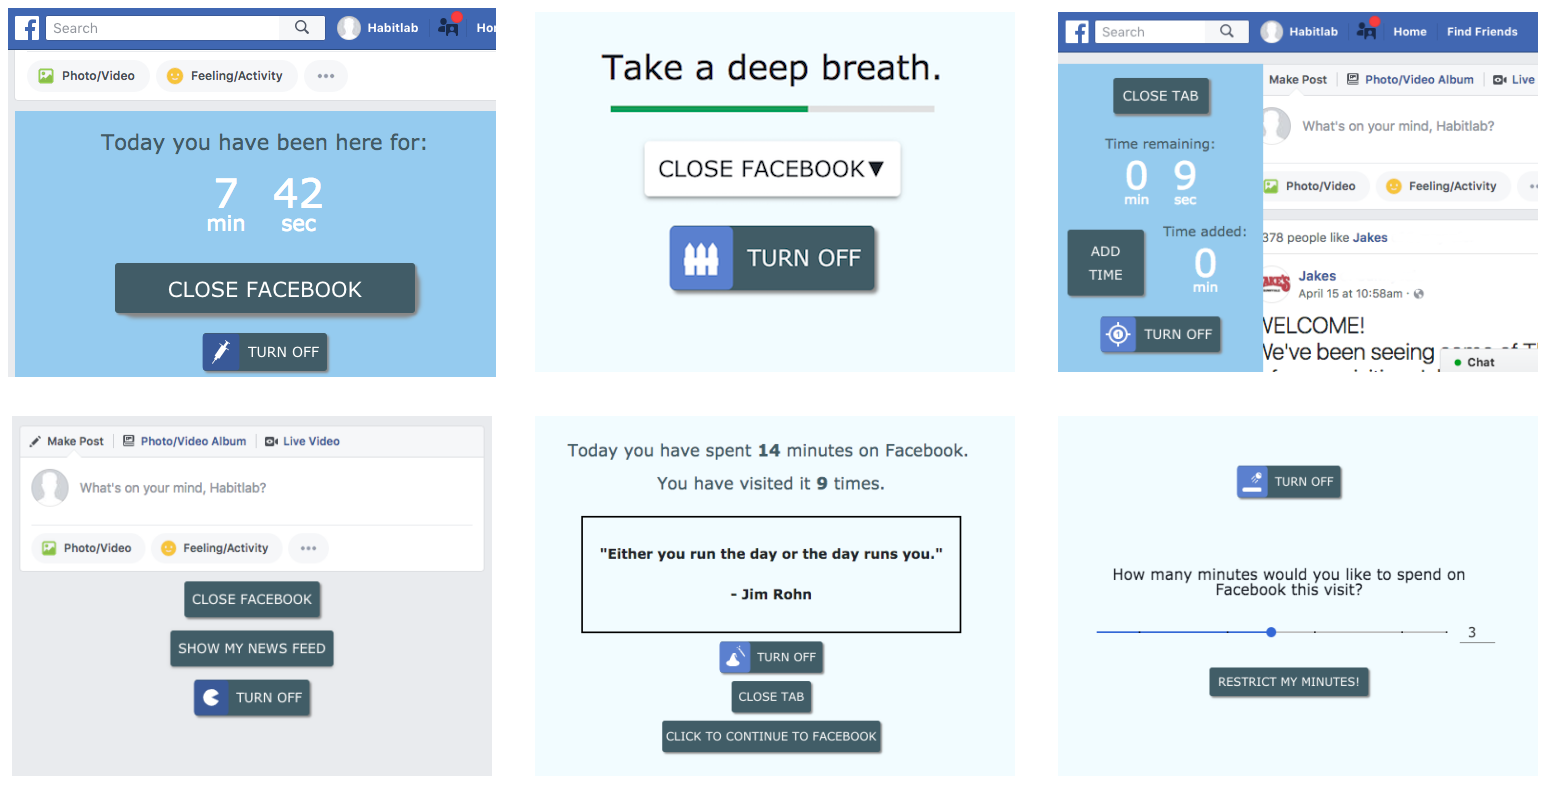
\includegraphics[width=1.0\textwidth]{figures/interventions_new.png}
	\caption{Examples of interventions available for reducing time on Facebook. From left to right, top to bottom: a timer injected into the news feed; a page before opening Facebook requiring that the user wait a few seconds before visiting; a countdown timer that automatically closes the tab after time elapses; an opt-in required to show the news feed; an interstitial page before opening Facebook with a quote; an interstitial page before opening Facebook that requires the user set a time limit for how long they will spend this session.}
\label{fig:interventions}
\end{figure}

\section{HabitLab adoption and usage}

As of writing, the browser version of HabitLab has over 12,000 daily active users from 85 countries (US, India, Germany, France, and the UK are the top 5), and volunteers have translated it into 9 languages (German, French, Spanish, Dutch, Portuguese, Chinese, Czech, Greek, and Turkish). The Android version has over 500 daily active users.

The users were not explicitly recruited, but were rather all organic installs who discovered the extension/app via sources such as the Chrome/Play store, or were referred to it via press coverage in sources such as Wired or the New York Times.

% Users discover the extension through news articles (it has been mentioned in Wired and the New York Times), the Chrome store, or links from an unrelated open-source project by the author.

Users are asked to read and provide consent to the research protocol upon installation. They may opt out of data collection if they do not wish to have their data analyzed for research purposes.

\section{User demographics}

TODO

\section{Design principles and tradeoffs}

We designed HabitLab from the start intending it to be a in-the-wild experimentation platform with a large number of users who would voluntarily and organically install it. As a result, we made a number of design decisions that prioritize growth and retention.

Interventions can all be disabled by the end user, either temporarily for the duration of a session via a "Turn off" button shown on each intervention, or permanently. This is intended to boost retention by preventing uninstalls caused by users disliking a particular intervention. While this complicates some analyses -- for instance, we may have fewer samples about the effectiveness of less popular interventions that tend to be disabled more -- we believe this to be the appropriate tradeoff.

Interventions are designed to be minimally intrusive. While in principle users can just disable interventions they do not like, we still found that many users would uninstall after seeing particular, intrusive interventions. We saw this pattern most notably with interventions that have interstitial screens -- that is, they prevent the user from interacting with the page until they have gone through the intervention. As a result, with the exception of a handful of interventions which must be in the interstitial format -- for instance, forcing the user to wait for 10 seconds before loading the page -- we tried to avoid interstitial interventions as much as possible.

Interventions are designed to load fast, and as a result we ensure that all interventions can work offline and do not depend on remote network resources that might take a long time to load. We found that for interventions that take a second to load or more, the uninstall rate would increase after seeing them. This effect is particularly evident with interstitial interventions, which would have the jarring effect of allowing the user to use the site for a few seconds and disrupting them with an interstitial page once the intervention loads.

We have a simple and short onboarding process. Notably, we do not have long demographic surveys that characterize other similar research projects like LabInTheWild, relying on data from Google Analytics to gather demographic data instead. While data from Google Analytics is only approximate -- it is estimated from browsing patterns rather than from asking users directly -- we believed that if the data is accurate enough to be used by market research companies worldwide, it would be adequate for our purposes. Furthermore, requiring users to complete onboarding demographic surveys would not be able to guarantee that users would answer truthfully.

This principle of minimizing the amount of questions the user must answer also extends beyond the onboarding process. We make only minimal usage of experience sampling. We do so because we saw in one of our studies that even minimally intrusive, single-click experience sampling prompts that users can safely ignore will significantly increase the uninstall rate. As a result, most of the data we are able to gather is quantitative in nature, and we are only able to gather limited qualitative data from what users report to us through email, our feedback pages, reviews left on app store pages, or the uninstall survey.

% shown in Figure \ref{fig:onboarding_nudges}, some ``generic'' interventions can be used on all sites, and others were developed specifically for a particular site such as Facebook or Youtube.

%\begin{figure}
%  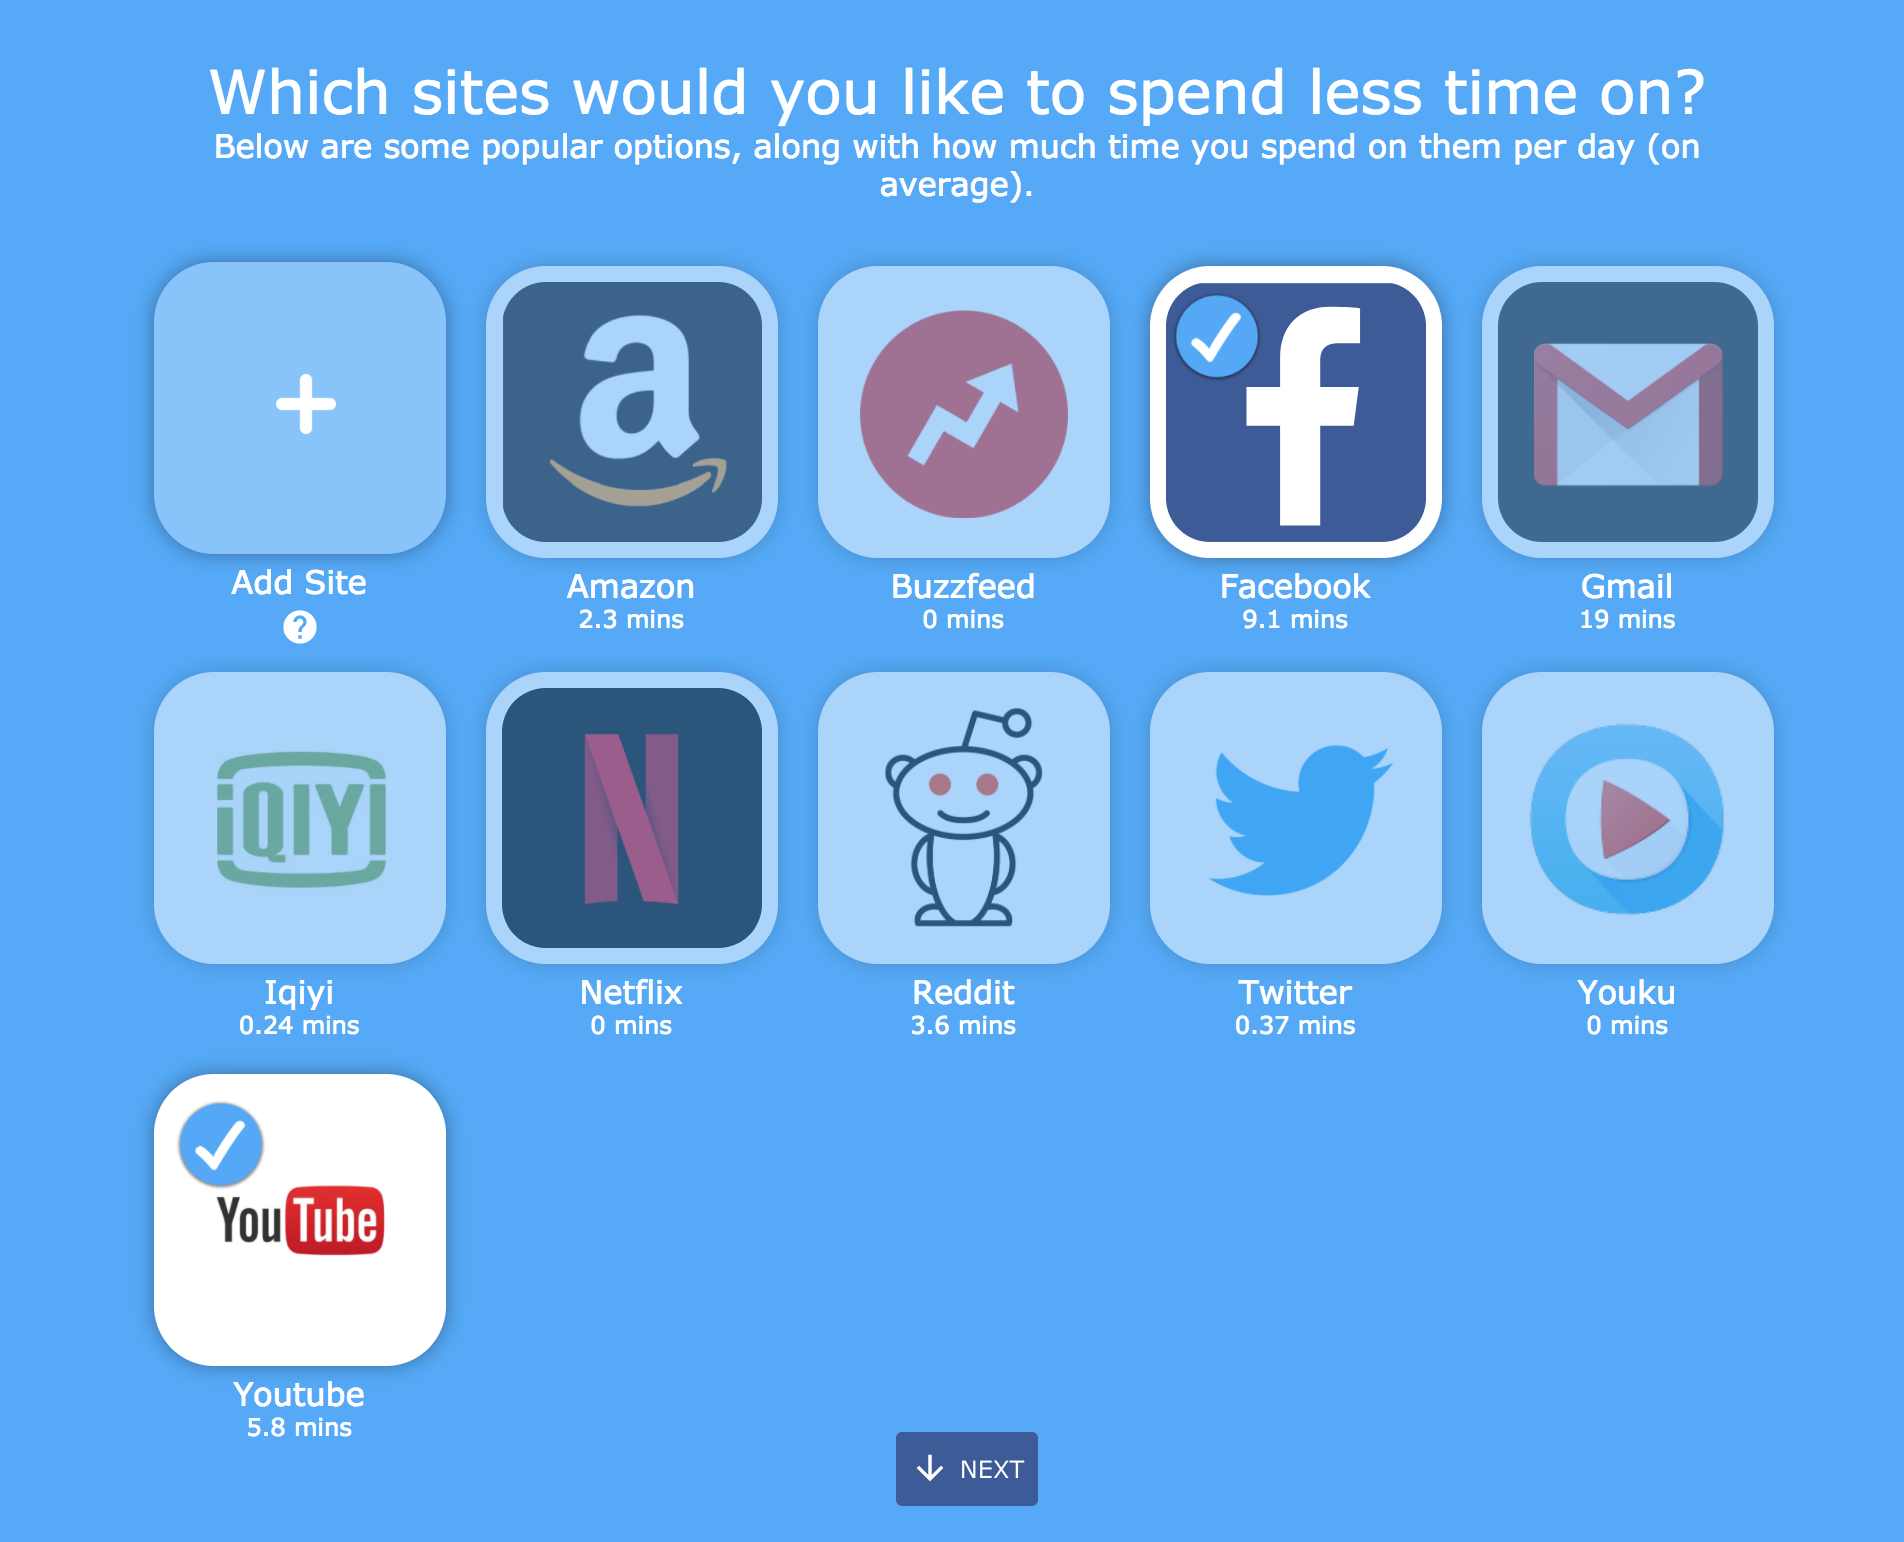
\includegraphics[width=\textwidth]{figures/onboarding_sites}
%  \caption{During onboarding, users first select sites to spend less time on.}
%  \label{fig:onboarding_sites}
%\end{figure}

%\begin{figure}
%  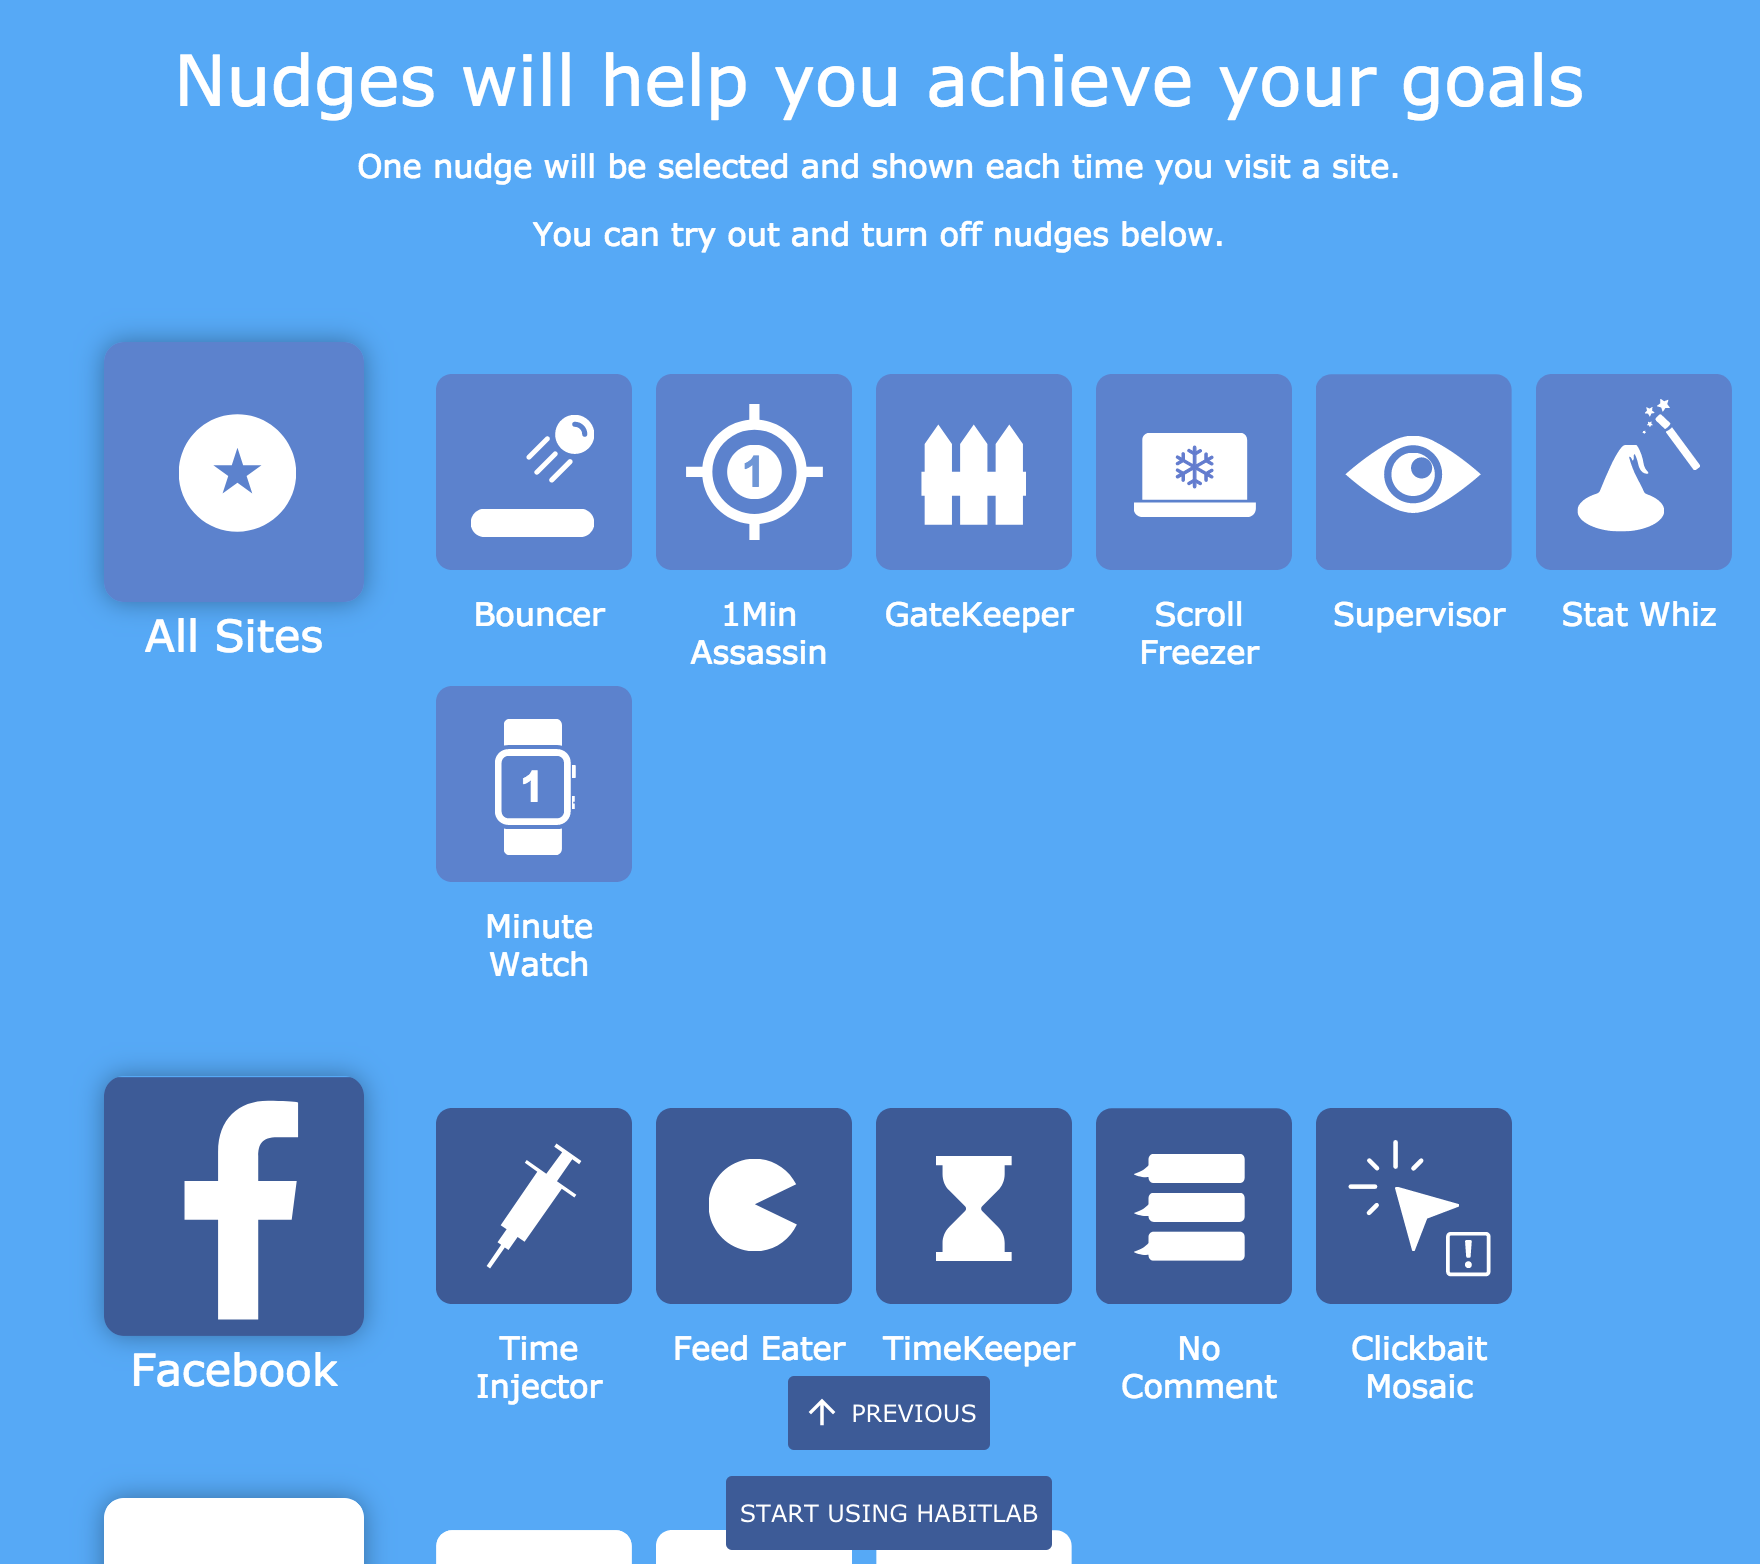
\includegraphics[width=\textwidth]{figures/onboarding_nudges_short}
%  \caption{Users are then presented with the nudges (interventions) they will see on each site.}
%  \label{fig:onboarding_nudges}
%\end{figure}




%
\section{Behavior Change Platform: HabitLab}

To gain insight into possible redistribution effects in behavior change, we created and deployed HabitLab~\cite{habitlab}, an open-source\footnote{HabitLab is available at \url{http://habitlab.github.io}.} platform which contains a variety of productivity interventions. Our prior work on HabitLab focused only on in-browser interventions, with the goal of studying intervention rotation strategies. With this paper, we track time redistribution and introduce an Android app, allowing us to track redistribution not just within platforms but across platform boundaries as well. 

\begin{figure}[tb]
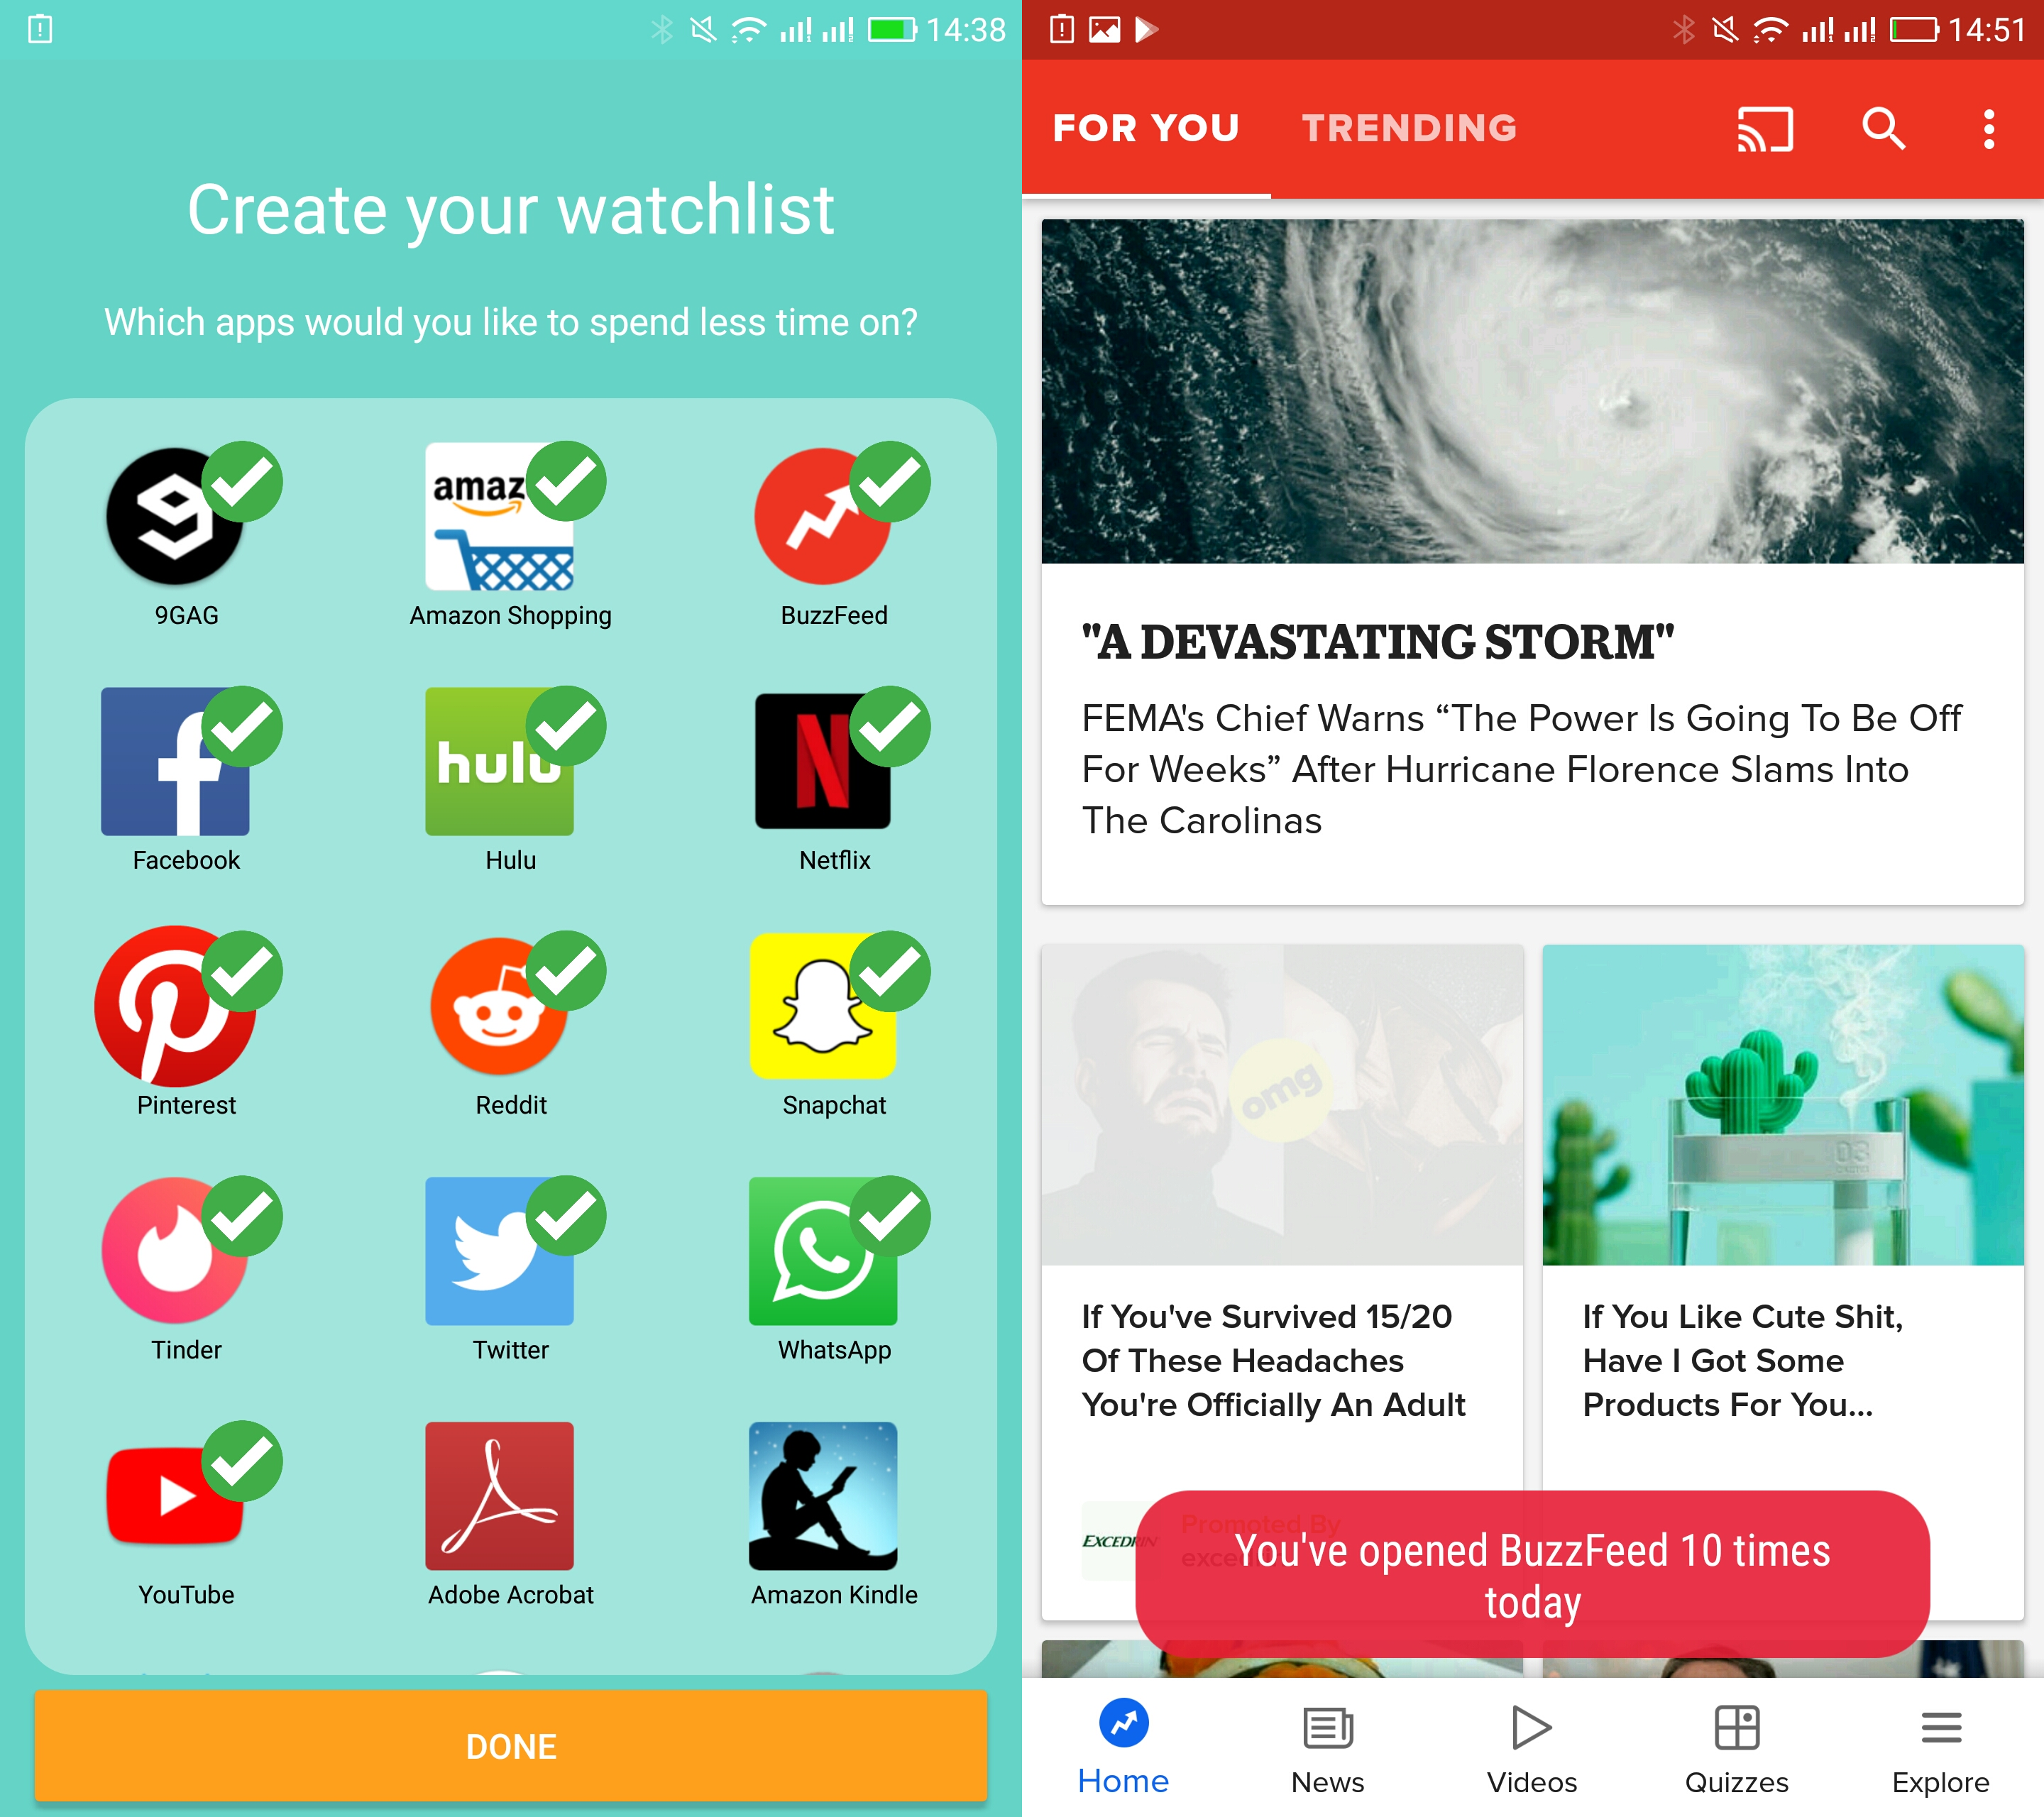
\includegraphics[width=\linewidth]{figures2/android_combined}
\caption{Screenshots from the mobile version of HabitLab.\\
Left: The goal selection screen, where users choose which apps to spend less time on.\\
Right: An example intervention, which shows the visit count when a user opens a goal app. %\msb{save space by cutting the image after the Iqiyi row. No point in having a nearly empty row at the bottom}
}
  \label{fig:android-goal-selection}
\end{figure}

% \begin{figure}[tb]
% \begin{minipage}[t]{0.49\linewidth}
% 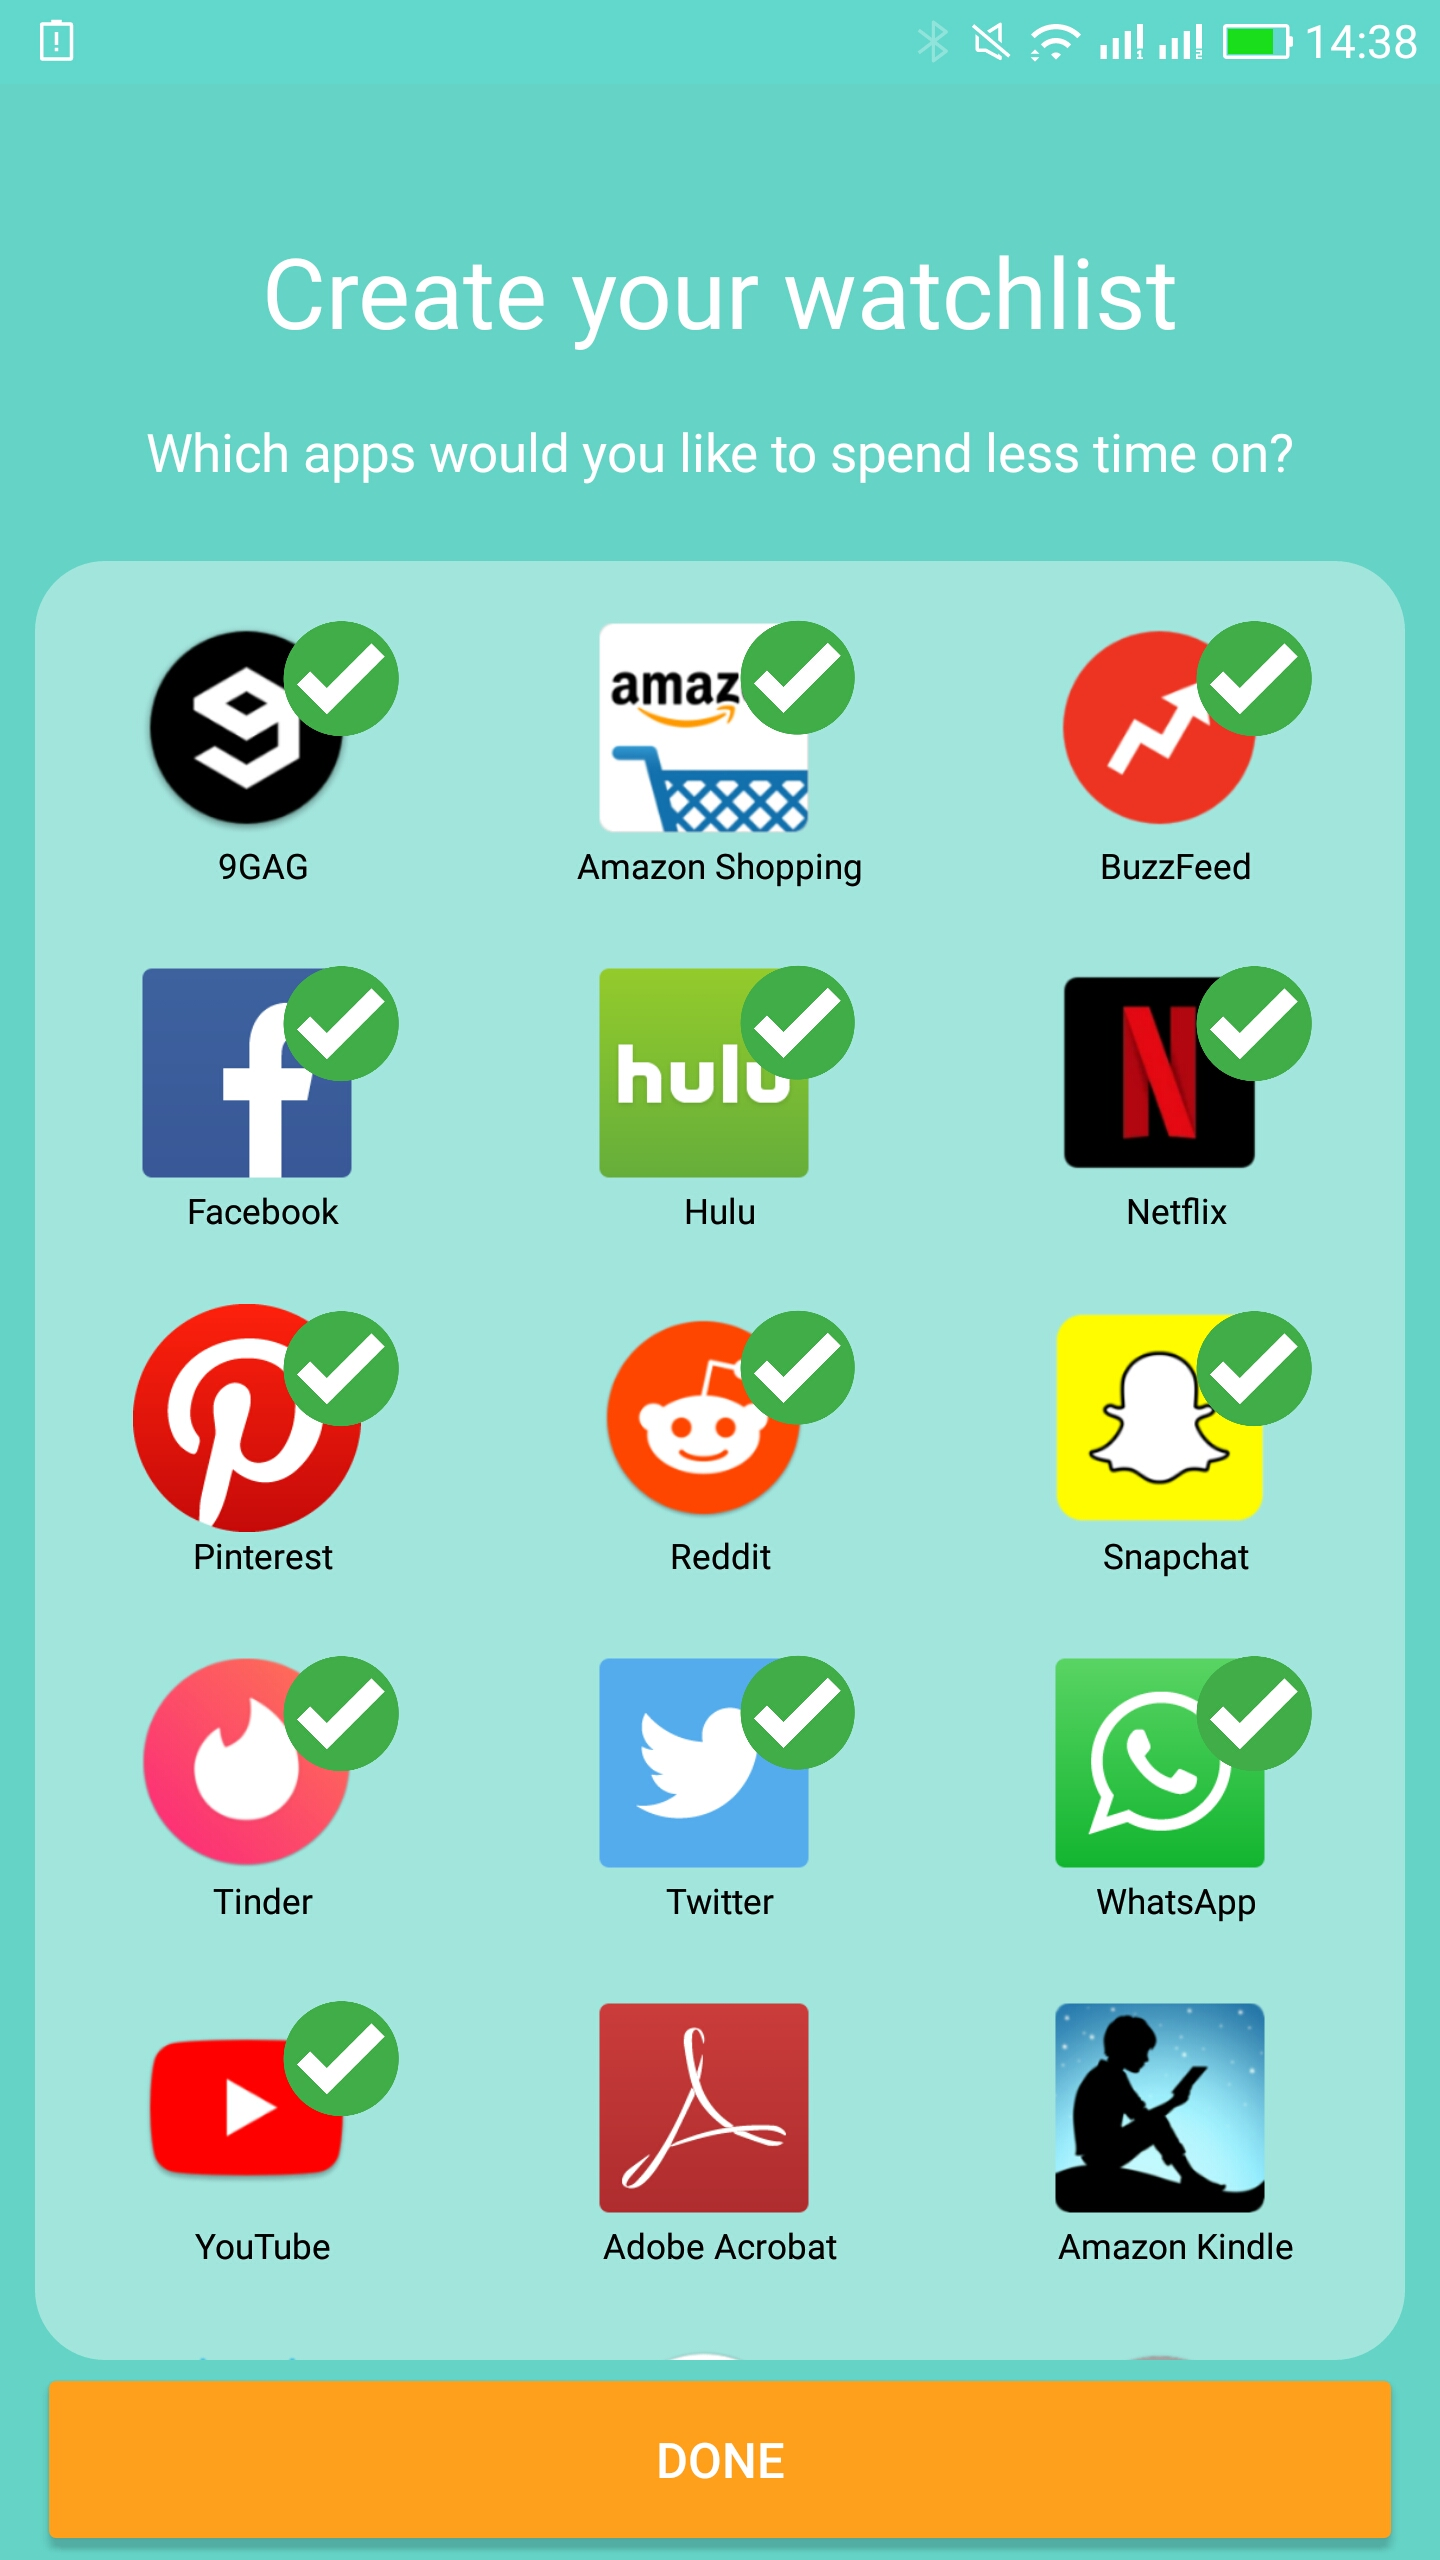
\includegraphics[width=\linewidth]{figures2/android-goal-selection}
% \caption{The goal selection screen, where users choose which apps to spend less time on (mobile version). %\msb{These two mini vertical figures are hard to read. Make it one figure with one caption underneath both.}
% }
%   \label{fig:android-goal-selection}
% \end{minipage}%
% \hfill
% \begin{minipage}[t]{0.49\linewidth}
% 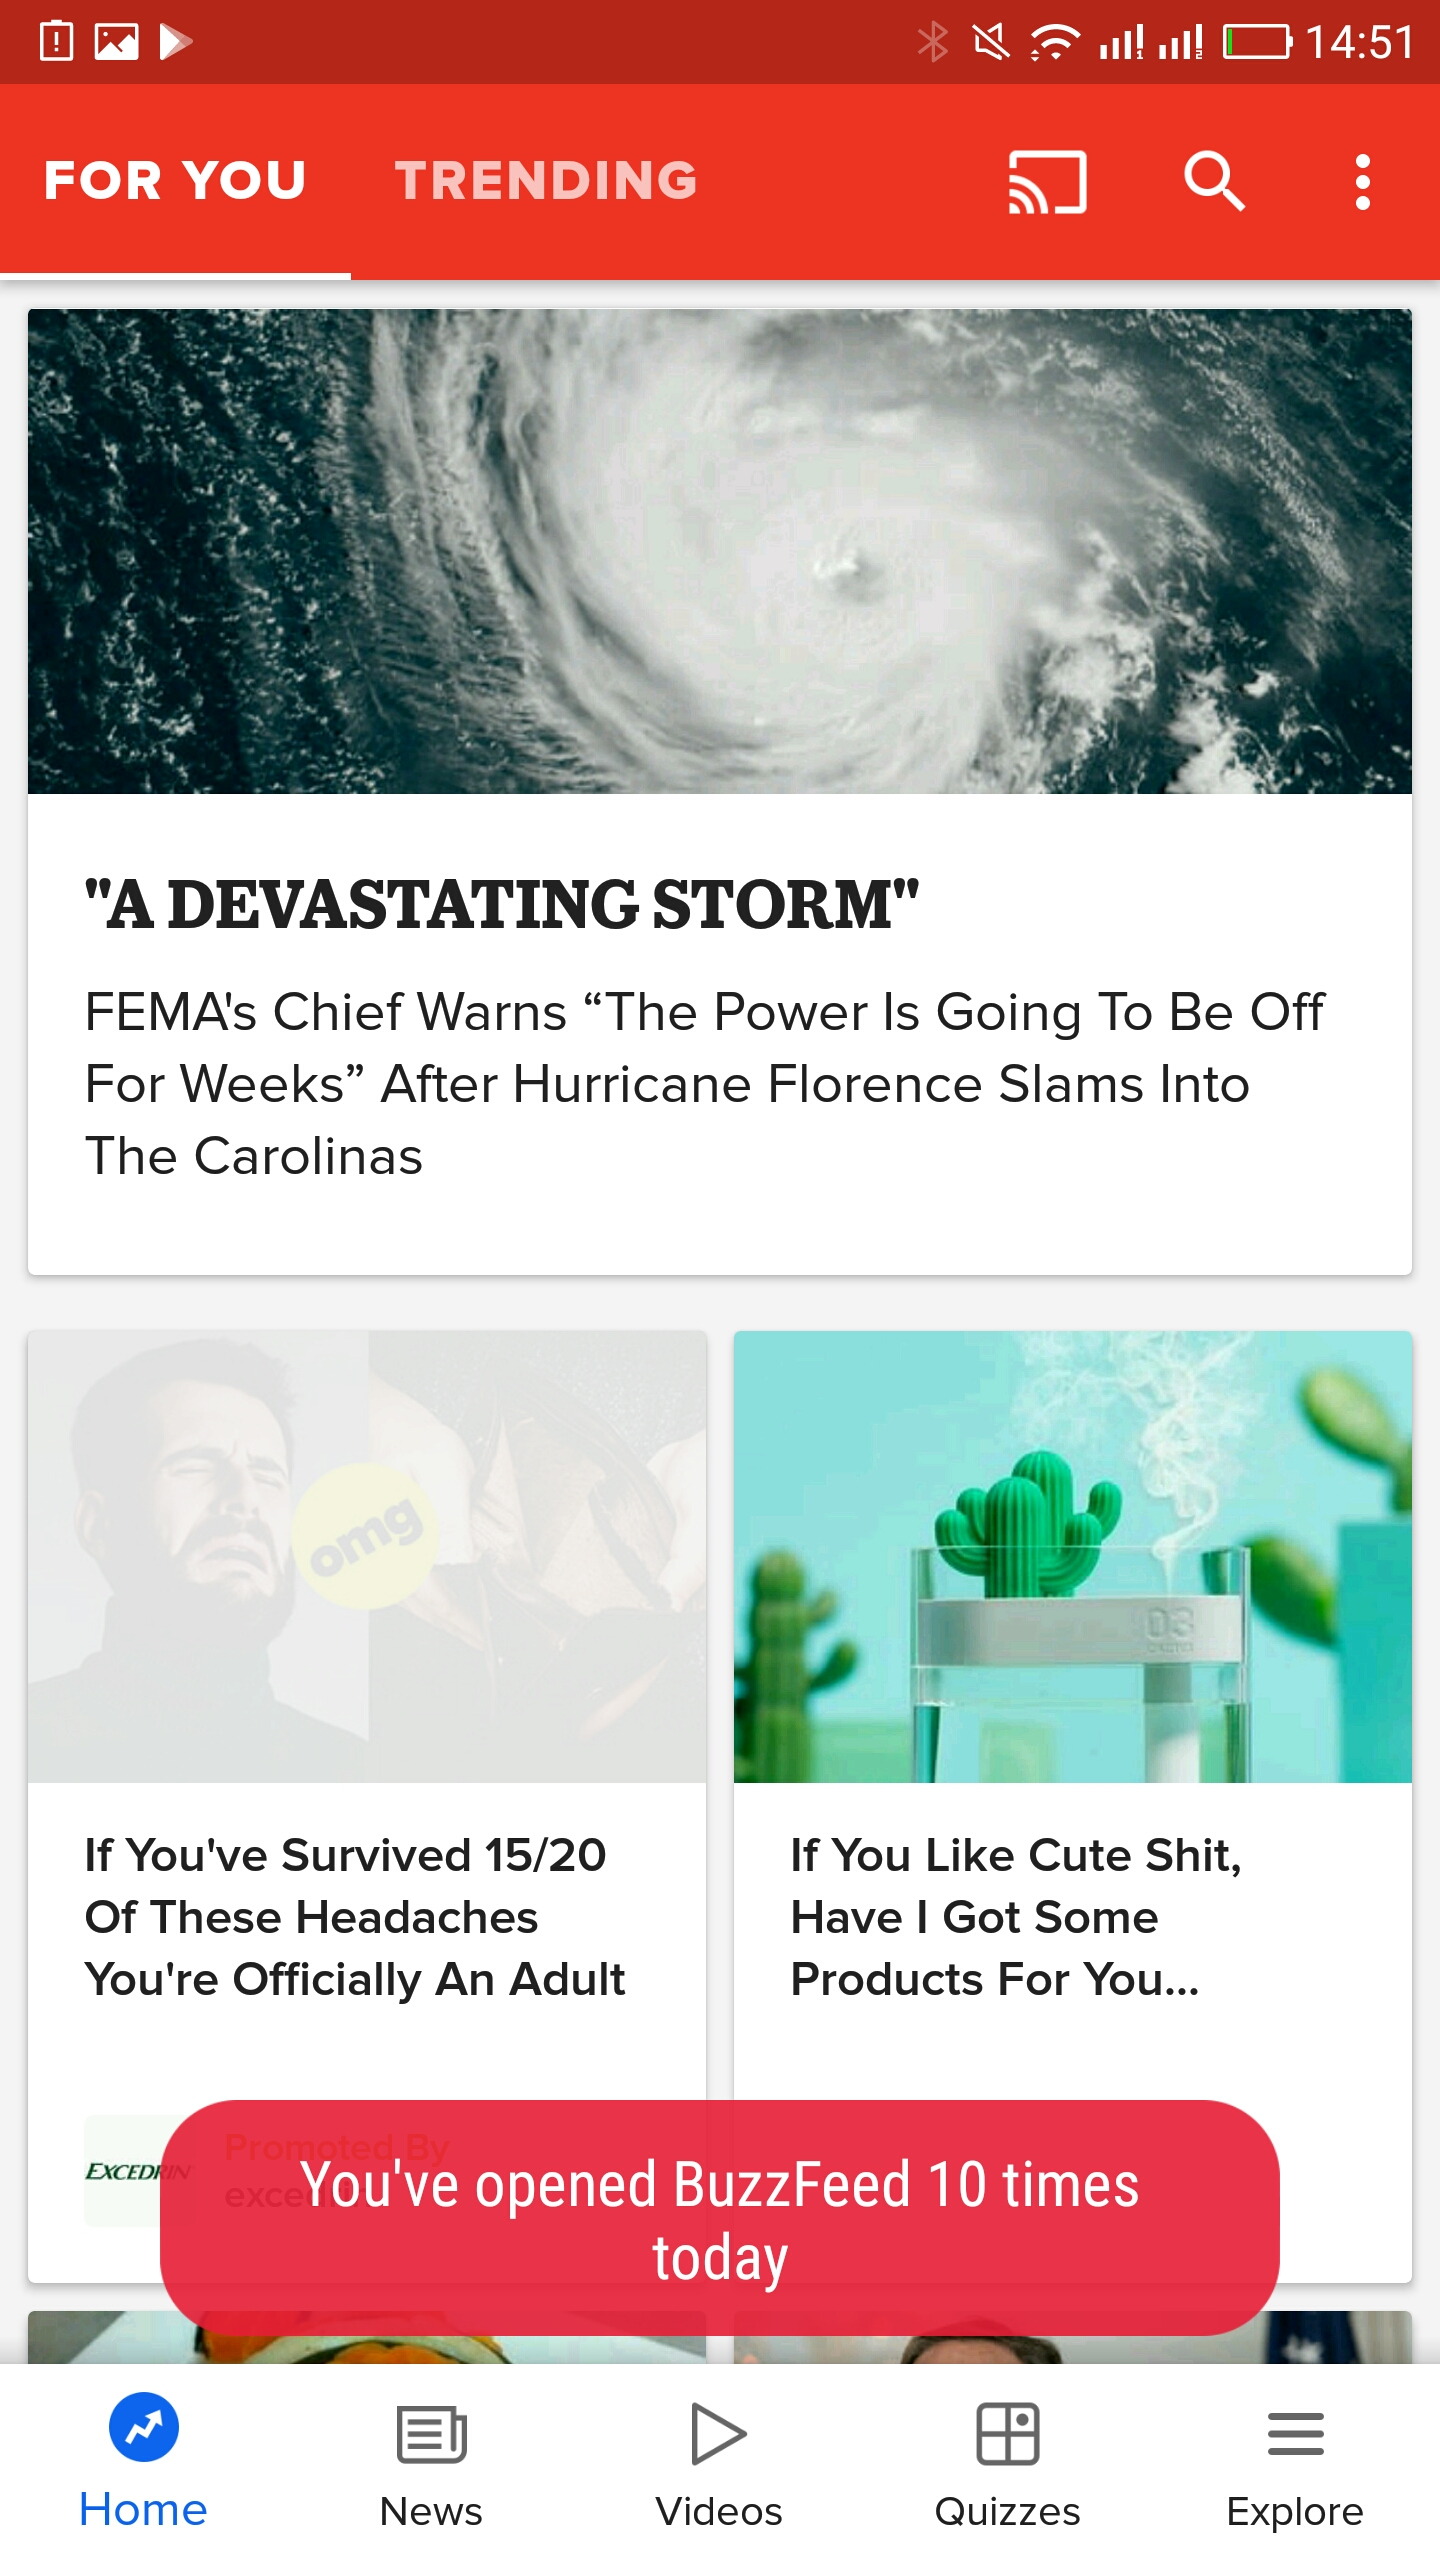
\includegraphics[width=\linewidth]{figures2/android-intervention}
% \caption{An example intervention, which shows the visit count when a user opens an app (mobile version).}
%   \label{fig:android-intervention}
% \end{minipage}
% \end{figure}

% \begin{figure}
% 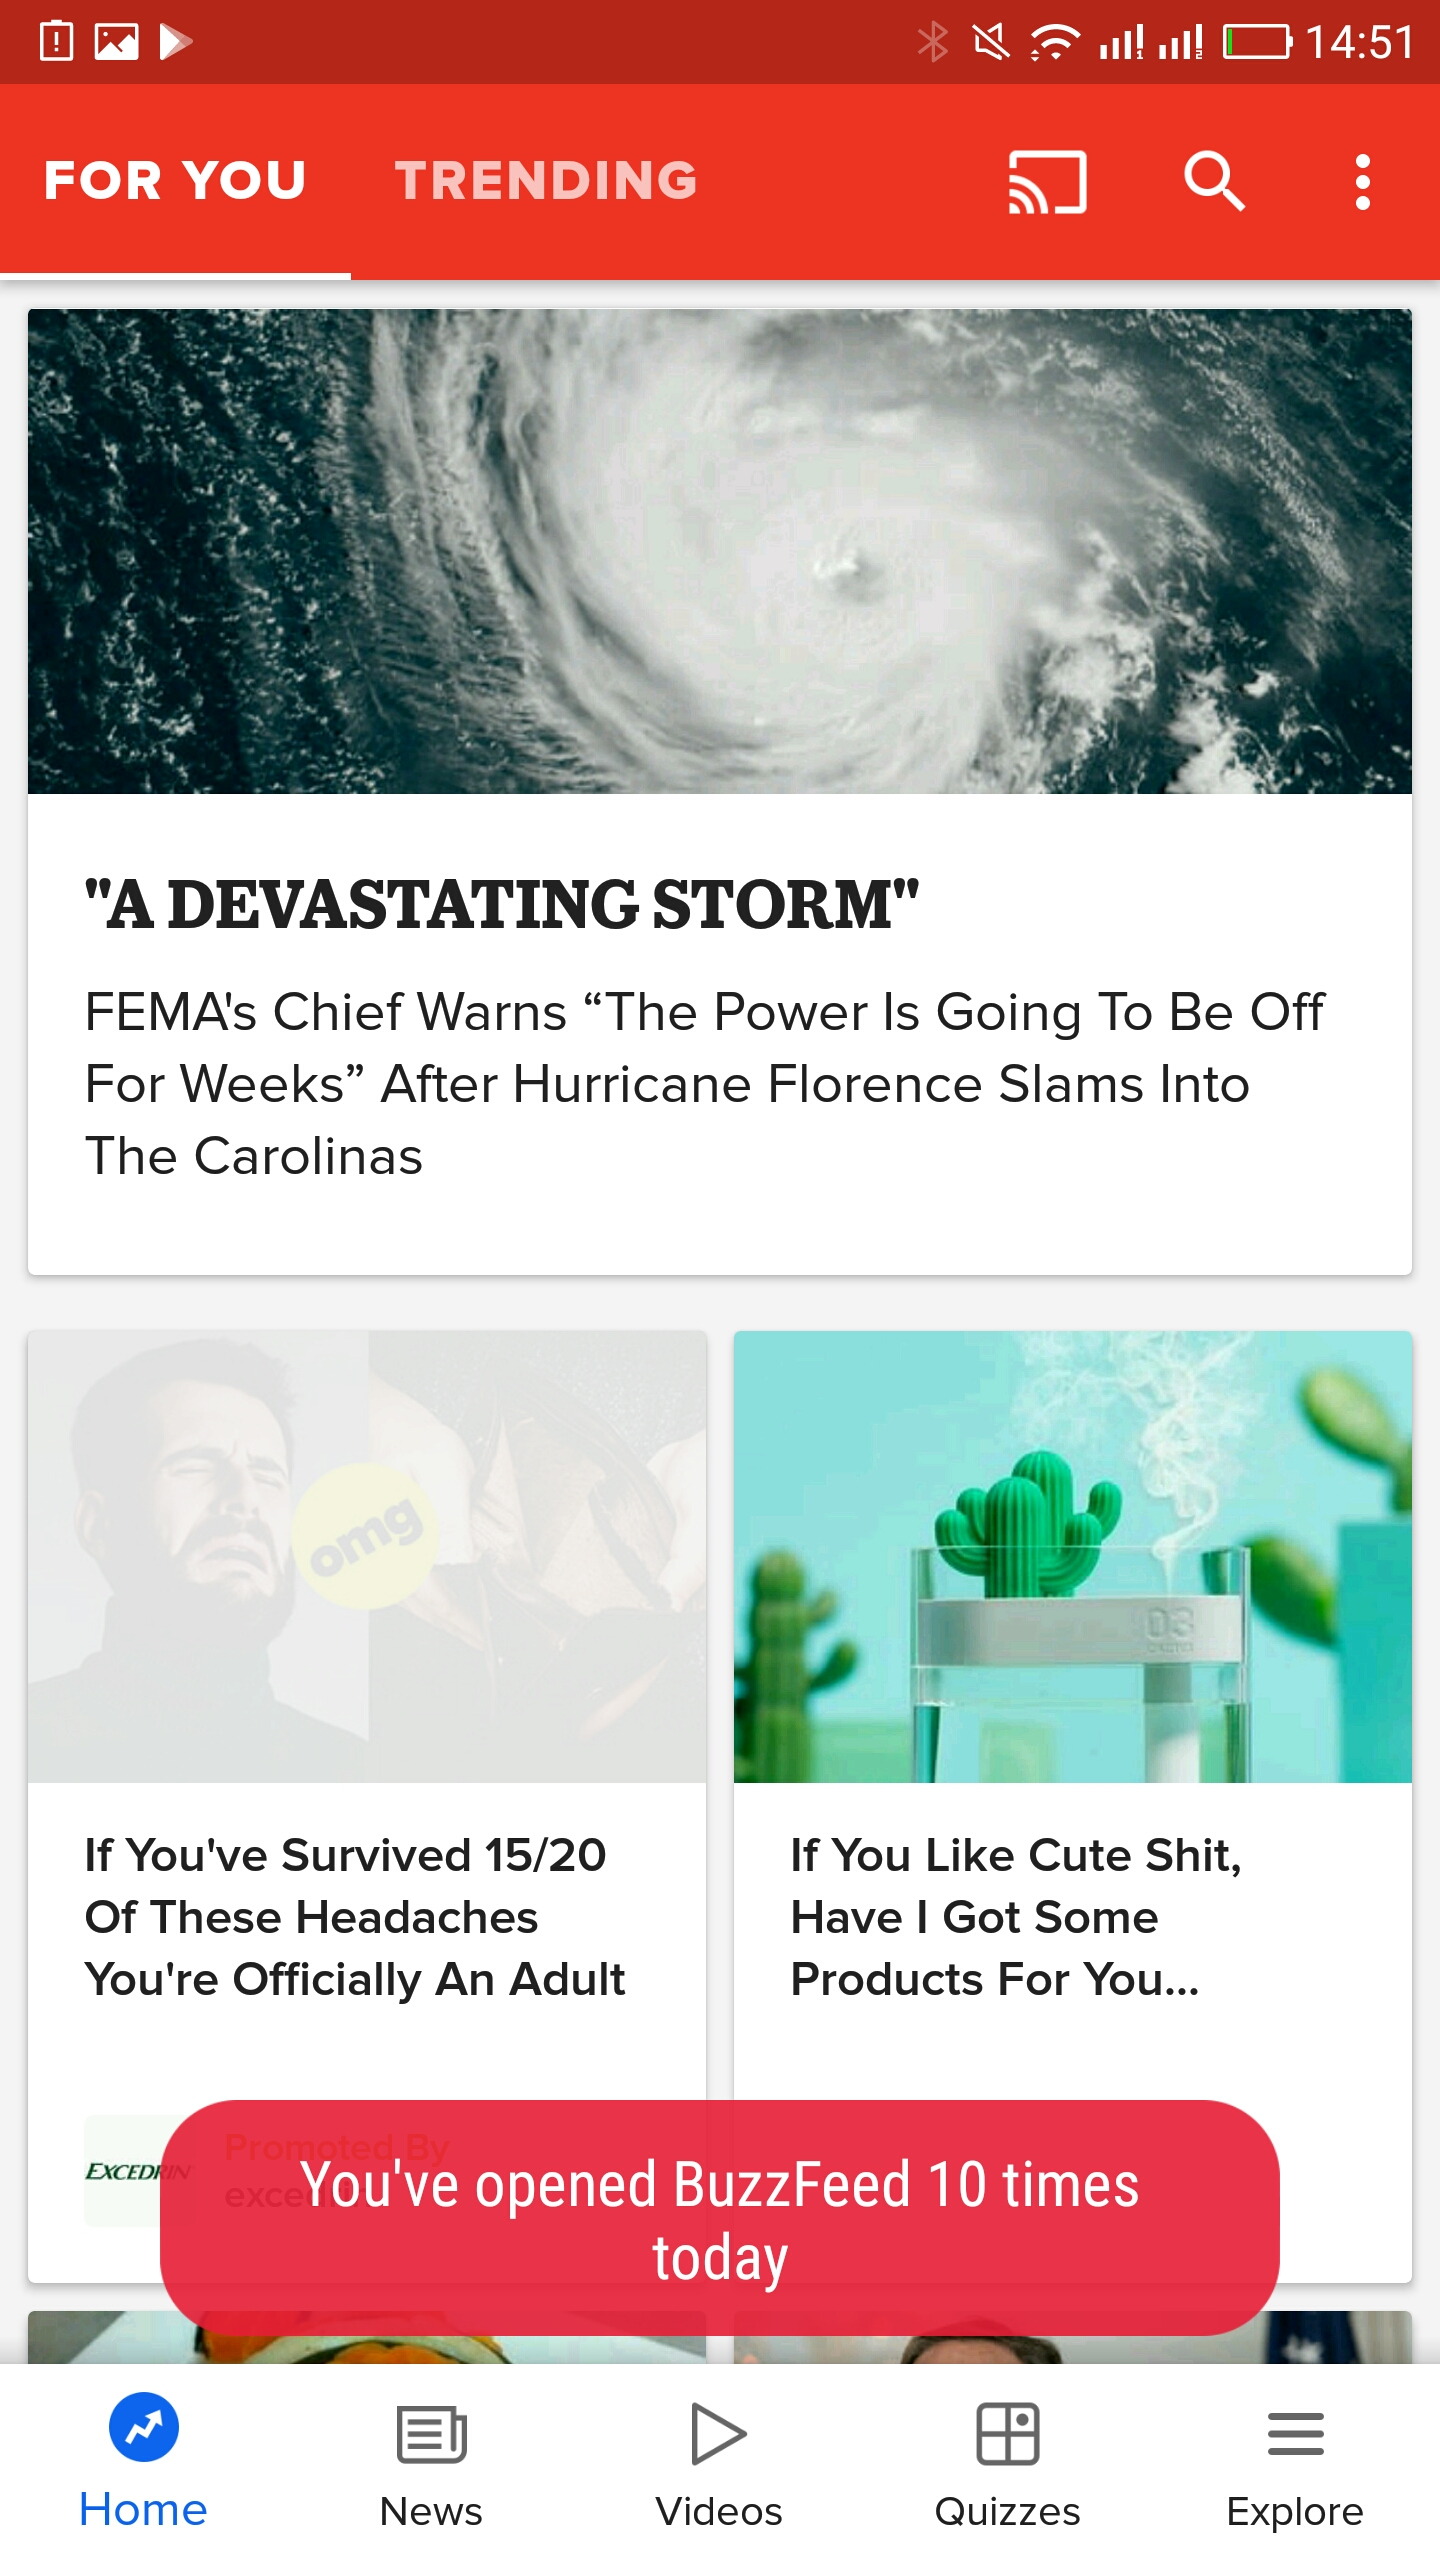
\includegraphics[width=\linewidth]{figures2/android-intervention}
% \caption{Mental model interface: each time the user sees a new intervention, HabitLab names it and explains about rotation.}
%   \label{fig:info}
% \hfill
% \includegraphics[width=\linewidth]{figures2/android-watchlist}
% \caption{User control interface: in addition to the mental model information, HabitLab gives users a direct interface to disable the new intervention.}
%   \label{fig:power}
% \end{figure}

\begin{figure}[tb]
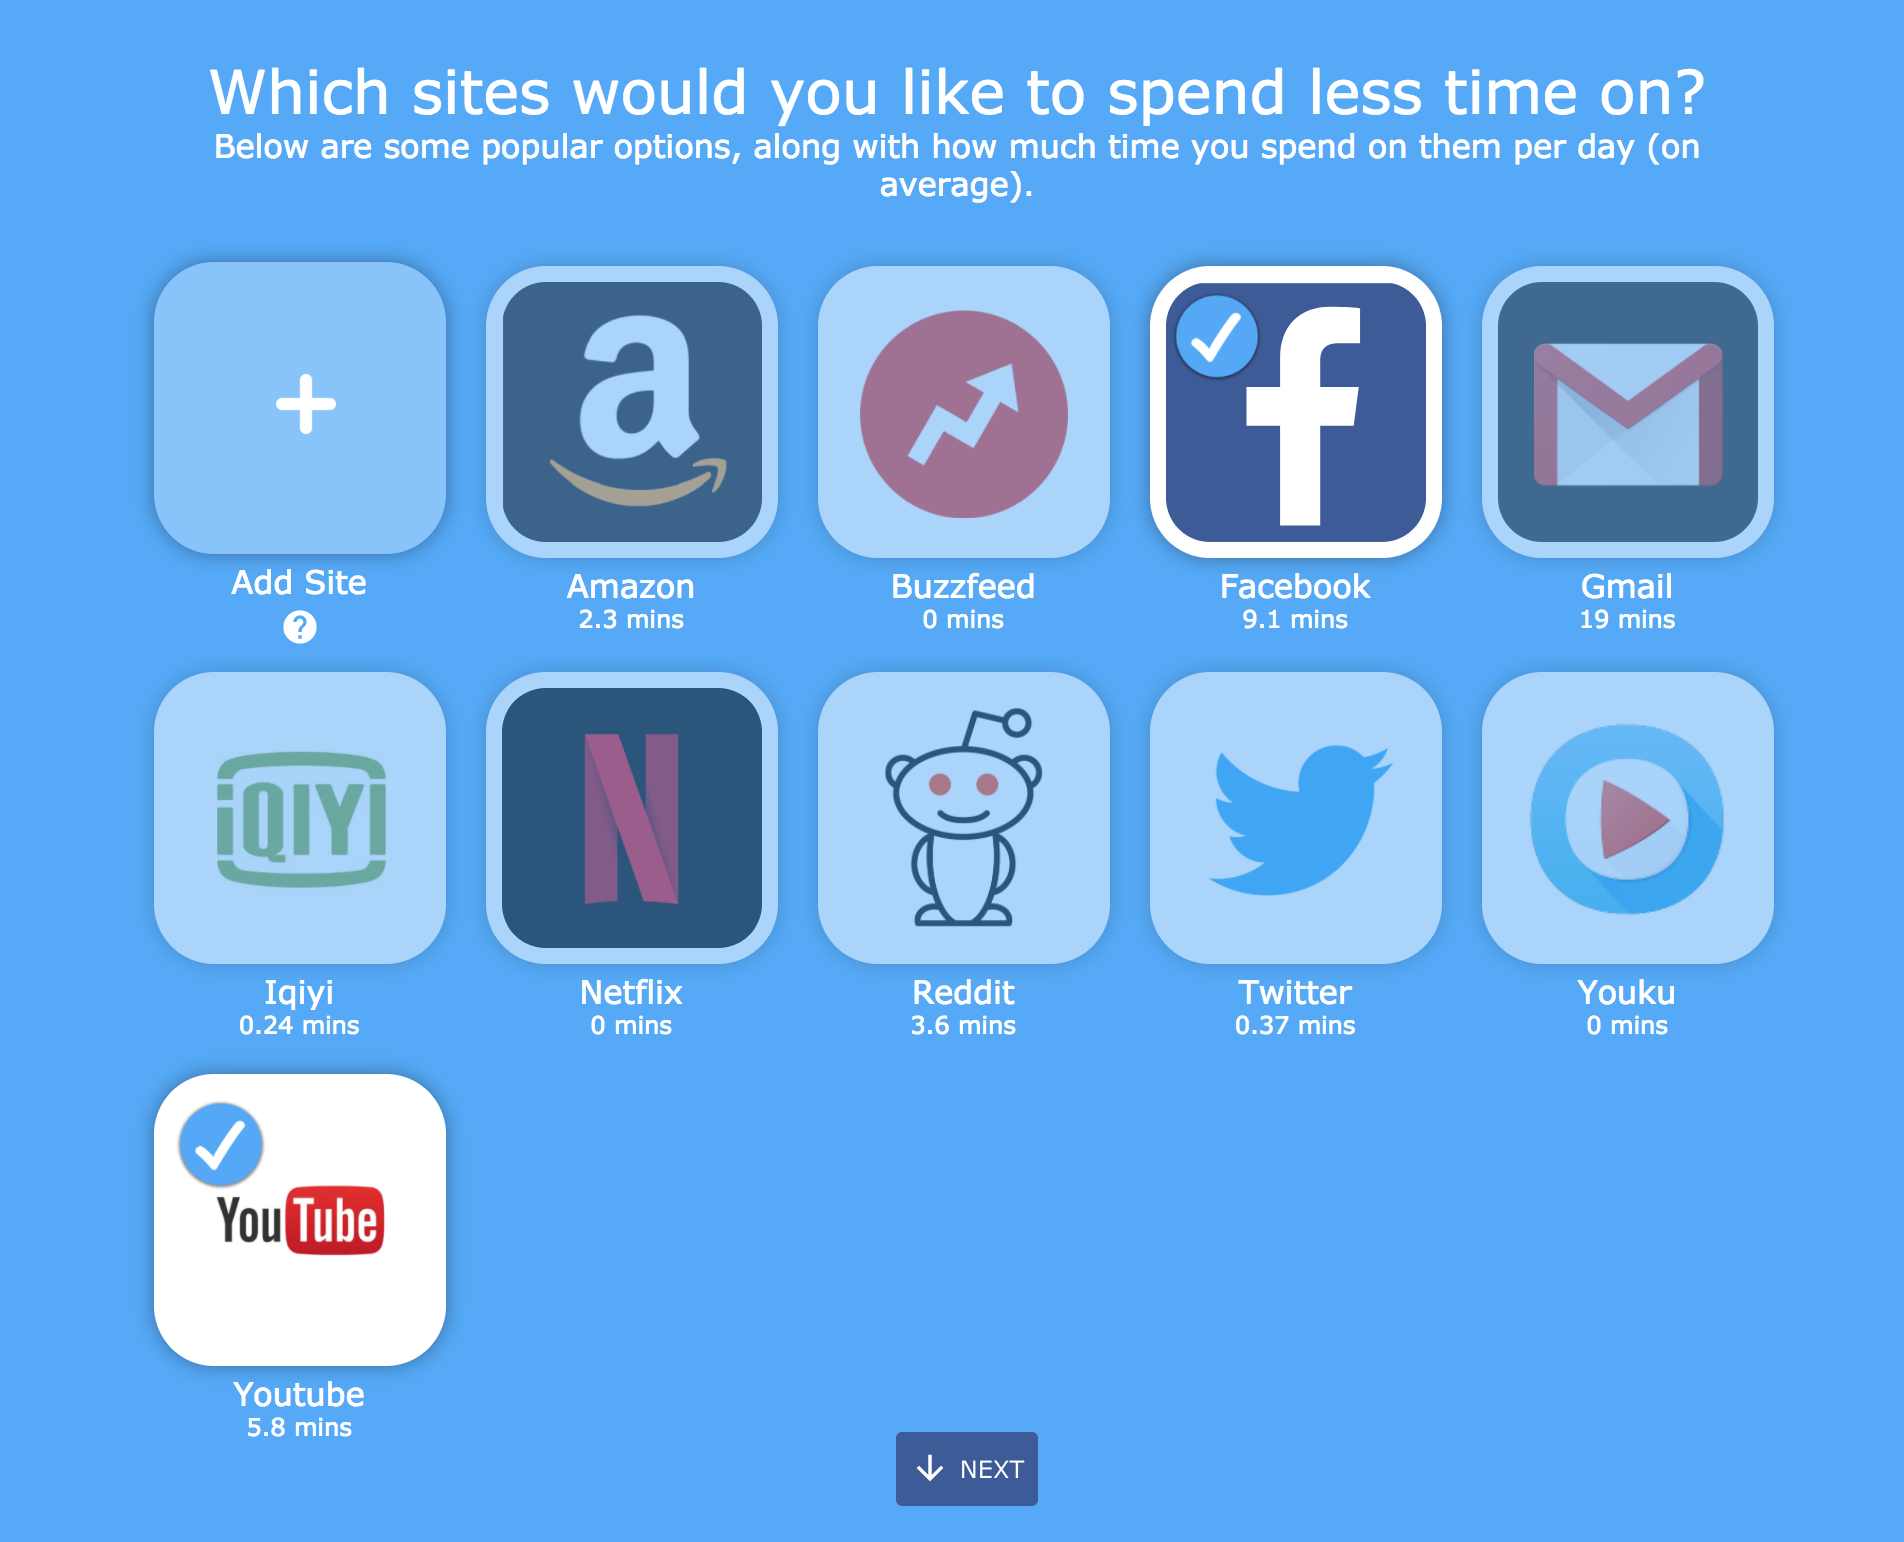
\includegraphics[width=\linewidth]{figures2/chrome-goal-selection}
\caption{The goal selection screen, where users choose which sites to spend less time on (browser version). %\msb{save space by cutting the image after the Iqiyi row. No point in having a nearly empty row at the bottom}
}
  \label{fig:chrome-goal-selection}
\end{figure}

\begin{figure}[tb]
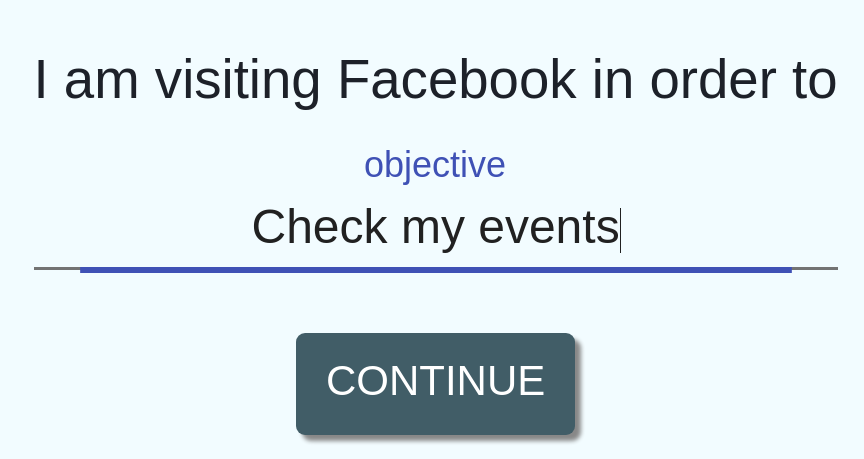
\includegraphics[width=\linewidth]{figures2/chrome-intervention-v3}
\caption{An example intervention, which asks a user to write their objective for visiting a site (browser version). %\msb{This page is really crowded with figures. I suggest moving one onto the next page.} 
% \msb{Save space by reducing this figure to start just above ``I am visiting FB to...''. The turn off button isn't necessary and it adds a ton of space to the paper.}
}
  \label{fig:chrome-intervention}
\end{figure}

There are two versions of HabitLab: a Chrome extension, and an Android app. Both follow the structure of allowing users to choose what they wish to spend less time on (setting goals), and deploying interventions to meet those goals. %The format of the goals differ between the two platforms.
On the Chrome version, users choose sites to spend less time on (goal sites -- for example, \url{facebook.com}), as shown in Figure~\ref{fig:chrome-goal-selection}. On Android, users choose particular apps to spend less time on (goal apps -- for example, the Facebook Android app), as shown in Figure~\ref{fig:android-goal-selection}. Interventions are deployed when users visit a goal site on Chrome (Figure~\ref{fig:chrome-intervention}), and when users open a goal app on Android, as shown in Figure~\ref{fig:android-goal-selection}.

%Particular interventions also differ between the platforms: the Chrome version includes a number of site-specific interventions such as a news feed remover for Facebook, whereas the Android version only has generic interventions that can be applied to all apps. The interventions are designed based on theories such as Cialdini's factors of influence~\cite{cialdini1987influence} and the behavior change wheel taxonomy of behavior change interventions~\cite{abraham2008taxonomy}. A complete list of interventions on the Chrome and Android versions along with descriptions can be found in the Appendix.

\section{Mobile and Browser version Differences}

The Chrome extension and Android app differ in some minor details. They support different sets of goals: users select apps to reduce time on in the Android version, whereas users choose sites to reduce time on in the Chrome version. Additionally, the specific set of interventions available differs between the platforms to fit the design languages of the browser and the mobile phone. The Chrome version has certain interventions which are site-specific -- such as a news feed remover that is specific to Facebook. However, because Android does not allow applications to edit each other's view trees, the Android version's interventions are all glass pane overlays, and thus are general and can be used on any app. The concept of a session is different on the platforms: in the Chrome version, a session is time on a site until that tab is either closed or the user goes to a different domain. Time measured is active time -- so if the tab is not focused, or if there is no keyboard or mouse activity for over a minute, the timer is temporarily paused. However, on Android, because there is no concept of a tab, the measurement of a session is different. There, a session is considered the duration over which an app is opened and focused. Closing the app, switching to a different app, or turning off the phone will end the current session.

%\subsection{Design of Interventions}

The design of HabitLab's interventions is based on theories such as Cialdini's factors of influence~\cite{cialdini1987influence} and the behavior change wheel taxonomy of behavior change interventions~\cite{abraham2008taxonomy}. Description of the interventions on the Chrome and Android versions can be found in the Appendix.



%\subsection{Userbase}

As of writing, the Chrome version has over 8000 daily active users, and the Android version has over 500 daily active users. The users were not explicitly recruited, but were rather all organic installs who discovered the extension/app via sources such as the Chrome/Play store, or were referred to it via press coverage in sources such as Wired or the New York Times.



\section{List of Browser Interventions}

% There are 27 interventions total: 7 generic interventions that can beused on all sites, 5 interventions designed specifically for Facebook, and additional ones designedspecifically for YouTube, Reddit, Twitter, Netflix, Gmail, Amazon, iQiyi, and Youku

The following is the list of interventions used for this study, showing the intervention name and description as seen by the end user.\\

Generic interventions that can be used on all sites:
\begin{small}
\begin{itemize}
    \item Minute Watch: Notifies you of time spent every minute
    \item Supervisor: Shows time spent on site at the top of screen
    \item Scroll Freezer: Freezes scrolling after a certain amount of scrolls
    \item Stat Whiz: Show time spent and visit count each visit
    \item GateKeeper: Makes you wait a few seconds before visiting
    \item 1Min Assassin: Closes tab after 60 seconds
    \item Bouncer: Asks how long you want to spend on site this visit
\end{itemize}
\end{small}
\vspace{2mm}

Facebook-specific interventions:

\begin{itemize}
    \item Time Injector: Injects timer into the Facebook feed
    \item Feed Eater: Removes the Facebook news feed
    \item TimeKeeper: Notifies you of time spent in the corner of your desktop
    \item No Comment: Removes Facebook comments
    \item Clickbait Mosaic: Removes clickbait from the news feed
\end{itemize}

\vspace{2mm}

Youtube-specific interventions:

\begin{itemize}
    \item Sidekicker: Remove sidebar links
    \item Think Twice: Prompt the user before watching a video
    \item No Comment: Removes comment section
\end{itemize}

\vspace{2mm}

Netflix-specific interventions:

\begin{itemize}
    \item Fun Facts: Gives you a fact and links an article on the effect of TV
    \item Alarm Clock: Asks the user to set an alarm before watching a show
    \item Stop Autoplay: Stops the site from automatically playing the next video
\end{itemize}

\vspace{2mm}

Reddit-specific interventions:

\begin{itemize}
    \item Comment Remover: Removes Reddit comments
    \item Mission Objective: Asks what you aim to do this visit and puts a reminder up
\end{itemize}

\vspace{2mm}

Youku-specific interventions

\begin{itemize}
    \item Think Twice: Prompt the user before watching a video
    \item Sidekicker: Remove sidebar links
\end{itemize}

\vspace{2mm}

iQiyi-specific interventions

\begin{itemize}
    \item Think Twice: Prompt the user before watching a video
    \item Sidekicker: Remove sidebar links
\end{itemize}

\vspace{2mm}

Twitter-specific interventions:

\begin{itemize}
    \item Feed Eater: Removes the Twitter news feed
\end{itemize}

\vspace{2mm}

Amazon-specific interventions:

\begin{itemize}
    \item No Recs: Hides recommendations
\end{itemize}

\vspace{2mm}

Gmail-specific interventions

\begin{itemize}
    \item Speedbump: Delays the arrival of new emails
\end{itemize}

\vspace{3mm}


\section{List of Mobile Interventions}

All mobile interventions are generic, that is they can be used on any app.

\begin{small}

\begin{itemize}
    \item At it Again: Sends a pop up with your app visit count.
    \item Progress Report: Sends a pop up with today's total usage for a certain app
    \item Red Alert!: Sends a notification with today's total usage for a certain app
    \item Repeat Offender: Sends a notification with your app visit count
    \item All in All: Pops a dialog with the day's total time on the current app
    \item Back To Target: Suggests you to visit a target app
    \item Counting on You: Puts a timer on screen in watchlisted apps
    \item Man Overboard! Shows a dialog with your app visit count
    \item No Peeking!: Asks for confirmation before opening watchlisted apps
    \item Wait Up! Pause for 10 seconds before entering an app
    \item Your Better Half: Sends a pop up to go to a target app
    \item Look on the Bright Side: Dim the screen a little at a time
    \item Take Your Pick: Select how long you want to spend on an app
    \item The Final Countdown: On screen timer that closes the app when time runs out
\end{itemize}

\end{small}


The following interventions apply across the device as a whole, not individual applications.

\begin{small}
\begin{itemize}
    \item How Time Flies!: Sends a pop up message with current app visit length
    \item Knock Knock: Sends a pop up with your glance count for the day
    \item Long Time No See: Sends pop up with your phone usage for the day
    \item Call it a Day: Sends notification with phone usage for the day
    \item Easy on the Eyes: Sends notification with glance count for the day
    \item Hello, Old Friend: Sends notification with unlock count for the day
    \item The Clock is Ticking: Sends a notification with the current app visit duration
    \item En Garde: Pops a dialog with the day's total unlock count
    \item Hold the Phone: Show dialog with phone usage for the day
    \item Long Story Short: Pops a dialog with the visit time for the current app
    \item Quote reminder: Show quote upon opening app
    \item Time Reminder: Show dialog with phone usage for the day
    \item Take Your Pick: Select how long you want to spend on an app
\end{itemize}
\end{small}

\section{User Feedback}

User feedback for HabitLab has been generally positive. On the Chrome store for the browser version, there are 26 reviews, with an average rating of 4.5 stars, while on the Play store for the mobile version, there are 24 reviews, with an average rating of 4 stars. Users leave us feedback, both positive and negative, in a number of forms -- through feedback forms within the interface, by filing issues on GitHub, or sending emails.

(Types of feedback and examples of them)

We find that some user feedback often request a specific intervention. A commonly requested feature is the ability to have multiple interventions active at once.  TODO

\msb{What kind of user feedback have we gotten?}

\msb{Would love to see a page of Discussion in this chapter. Possible topics include: (1) Do you think the same design principles would allow a research system to succeed in other domains? If so, why? If not, why not? (2) What did we try that didn't work, and why? (3) Of the stuff that you did in designing HabitLab, what do you think is the most central novel idea?}


\section{User Feedback}

%\msb{What kind of user feedback have we gotten?} \geza{done}

User feedback for HabitLab has been generally positive. On the Chrome store for the browser version, there are 26 reviews, with an average rating of 4.5 stars, while on the Play store for the mobile version, there are 24 reviews, with an average rating of 4 stars. Users leave us feedback, both positive and negative, in a number of forms -- through feedback forms within the interface, as shown in Figure~\ref{fig:feedback_form}, by filing issues on GitHub, or sending emails. A complete list of feedback that users agreed to have publicly shared is in Appendix~\ref{ch:github}.

\begin{figure}
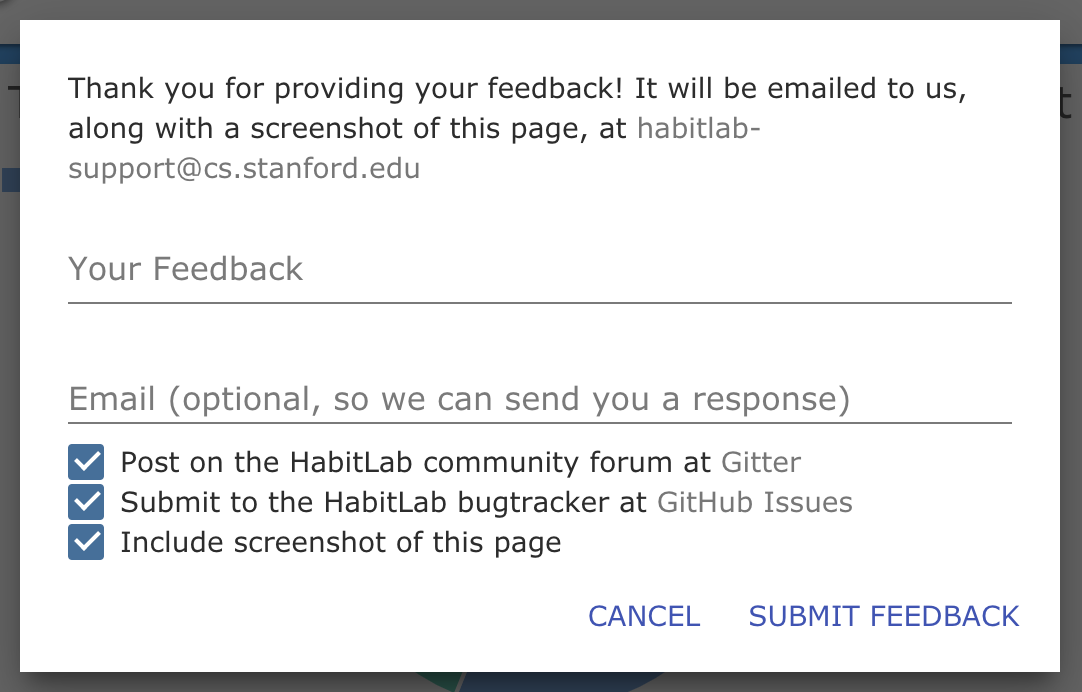
\includegraphics[width=\linewidth]{figuresS/feedback_form}
\caption{Our interface for submitting feedback within HabitLab.}
  \label{fig:feedback_form}
\end{figure}

%(Types of feedback and examples of them)

We find that most user feedback falls into the following categories:

\begin{itemize}
\item Requests:
\begin{itemize}
\item Requests for additional interventions
\item Requests for additional features and ways to customize the system
\item Requests for additional visualizations in the dashboard
\item Requests for site-specific functionality
\end{itemize}
\item Complaints:
\begin{itemize}
\item Complaints about resource usage
\item Complaints about particular interventions
\item Complaints about experience sampling
\item Complaints resulting from A/B testing and experimentation
\item Complaints due to user misunderstanding caused by excessive configurability
\end{itemize}
\item Positive feedback
\end{itemize}

\subsection{Requests}

\subsubsection{Requests for additional interventions}

We find that user feedback often request a specific intervention. Many are site-specific interventions. A commonly requested feature is to have combinations of interventions, or the ability to have multiple interventions active at once. We decided not to go down this path for two reasons:

\begin{itemize}
\item There is an exponential number of possible intervention combinations -- specifically, there are $2^n$ subsets of a group of n interventions. Thus, quantifying the effectiveness of combinations of interventions would take considerably more data than quantifying the effectiveness of individual interventions.
\item Some combinations of interventions would not work, provide a poor user experience, or would make little sense. For instance, it would make no sense to combine an intervention that injects items into feeds, with an intervention that removes feeds. To avoid deploying these to users, we would have to test and specify which particular subsets of interventions make sense to have together -- which, given that there an exponential number of possible intervention combinations, would take considerable effort.
\end{itemize}

Some examples of feedback of this form:

\textit{I think it would be great if there was the option for greater control to select multiple nudges to function every time. In my scenario, the website I want to control is Youtube. I use Youtube a lot whilst I'm working and being productive for various tutorials, downloading copyright fee assets and so on. However, the recommended videos often push click bait "trending" content at me, and having gone on Youtube to find a tutorial on solving a certain problem, you suddenly find your self 5 minutes into a "You won't BELIEVE what Gordan Ramsey says to this Chef" or similar rubbish. I'd really like to be able to use the Feed Diet, Sidekicker, Supervisor, and No Comment at the same time. I feel like your app has everything I need, but I can't use it all at the same time :)} -- \url{https://github.com/habitlab/habitlab/issues/641}

\textit{Youtube nudges not working as expected. Sidebar and comments turned on and showing normally. How many nudges can I active simultaneuosly?} -- \url{https://github.com/habitlab/habitlab/issues/620}

Users also often request new ideas for interventions. The following are some intervention ideas which were submitted via GitHub. The majority of ideas, however, are submitted via the idea voting interface in HabitLab, shown in Figure~\ref{fig:idea_voting} and are shown in Appendix~\ref{ch:ideas}.

\begin{figure}
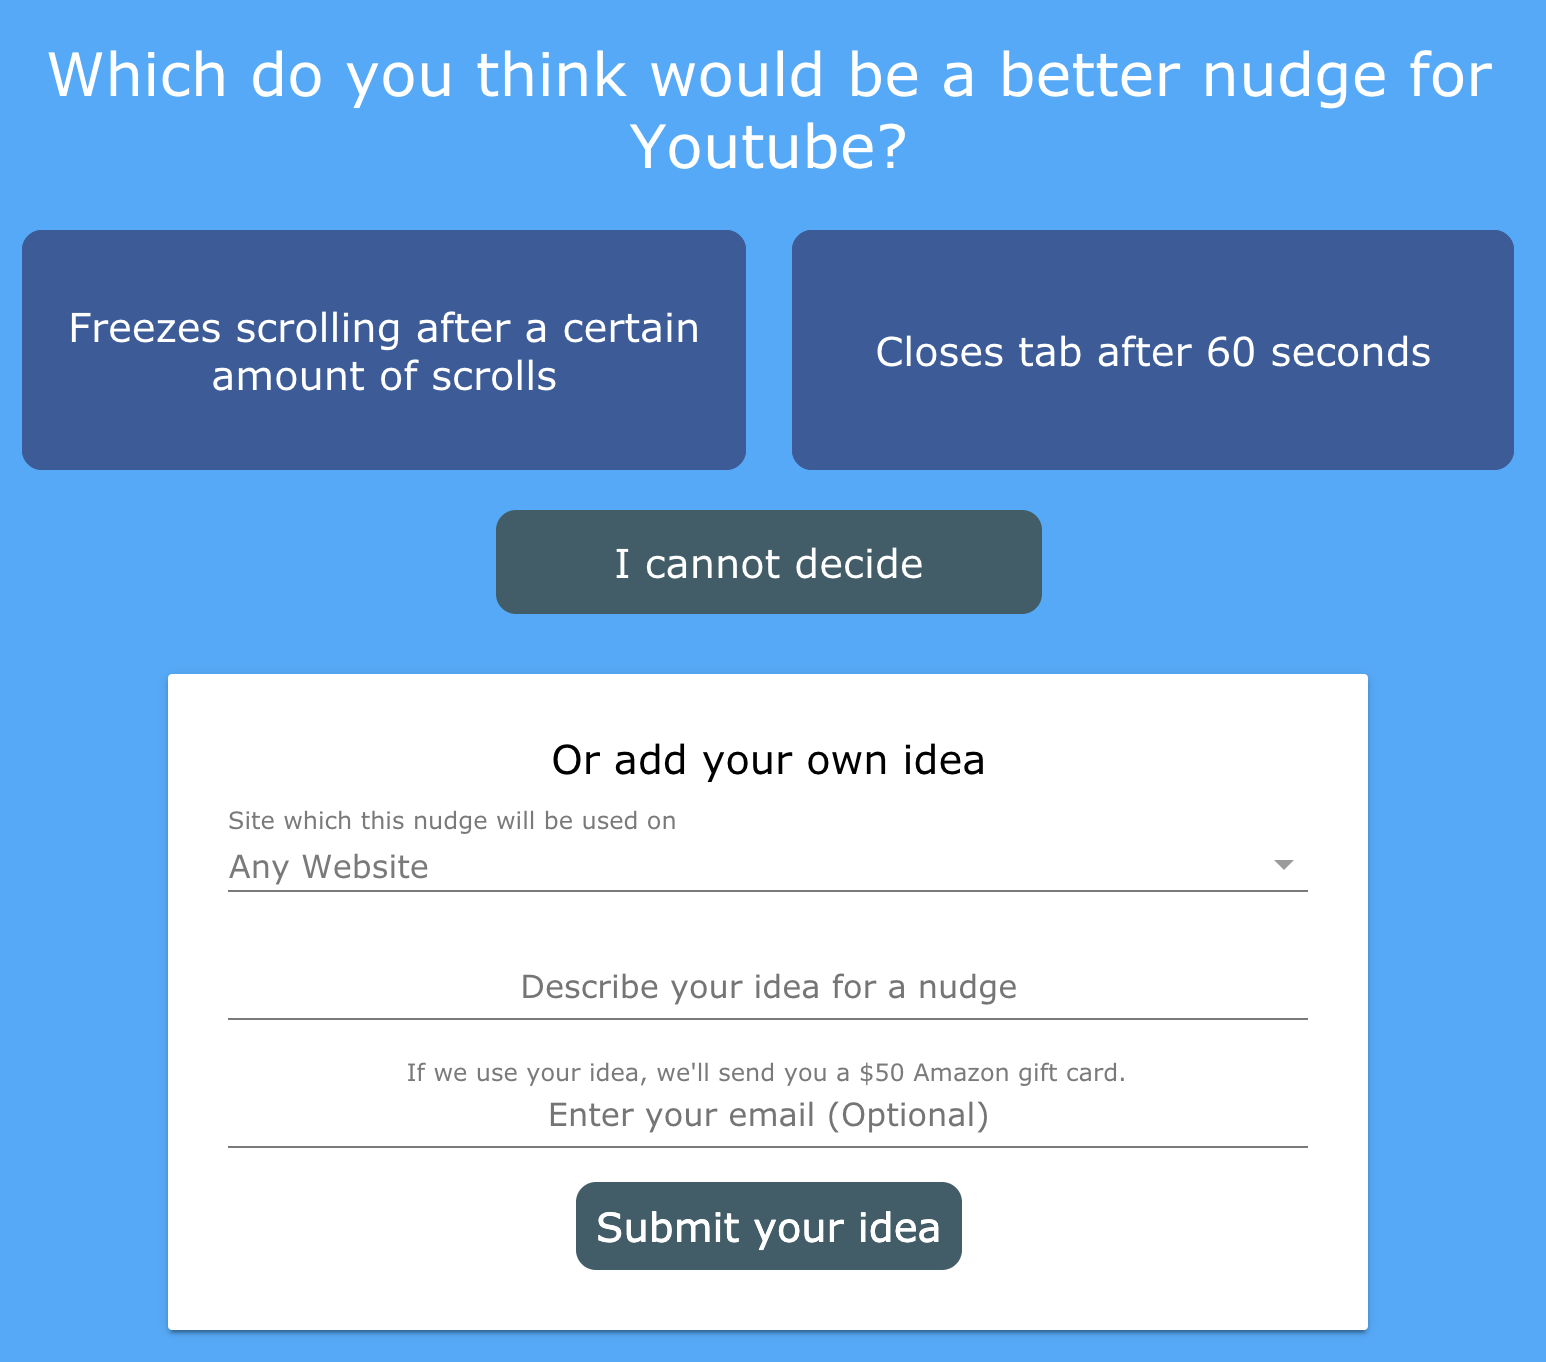
\includegraphics[width=\linewidth]{figuresS/idea_voting}
\caption{Our interface for letting users submit new intervention ideas and vote for existingones.}
  \label{fig:idea_voting}
\end{figure}

\textit{i would like to suggest maybe you can make another tracking nudge that only allows you to stay on a certain website and cant open any other tabs} -- \url{https://github.com/habitlab/habitlab/issues/593}

\textit{Hey! Would be nice to have displayed the total amount of time spent on the web. Great work, people! Thank you for making this :)} -- \url{https://github.com/habitlab/habitlab/issues/627}

\textit{Start making font (and other content) fade to grey with each scroll. Slowly the font will become tougher and tougher to read.} -- \url{https://github.com/habitlab/habitlab/issues/512}

\textit{nudge ``1 min assassin'' that decreases to e.g. 30sec assasin if you already spent 10 minutes on the domain} -- \url{https://github.com/habitlab/habitlab/issues/536}

\subsubsection{Requests for additional features and ways to customize the system}

Another commonly-seen request is for additional features and the ability to customize certain aspects of the program.

A commonly requested feature is the ability to turn off the ``Turn Off'' button which is present in each intervention.

\textit{Option to hide ``Turn off HabitLab'' button.} \url{https://github.com/habitlab/habitlab/issues/605}

\textit{Please add an option in settings to hide nudge turn off buttons (so they can only be turned off from settings page).} -- \url{https://github.com/habitlab/habitlab/issues/604}

\textit{Please allow option to not turn off buttons, e.g. "turn off feed eater button". Ideally this is a global option across all extensions. Thanks! :)} -- \url{https://github.com/habitlab/habitlab/issues/361}

Some users request more flexibility in which interventions are shown in particular contexts:

\textit{In general, I think the random is a good idea, but I quickly realize some of the random ones are ineffective for me. Rather than the random, it would be great if I could designate 1 feature for a particular website. For example, I know that facebook is a big time waster to me and moreso than others. I would love it if that was 1 one minute kick-off no matter what. Others (eg - Twitter) are less of a distraction for me, so the random wouldn't be as painful.} -- \url{https://github.com/habitlab/habitlab/issues/583}

\textit{have multiple slots for work times. eg : 8h00 12h00 and 14h00 18h00} -- \url{https://github.com/habitlab/habitlab/issues/533}

Some users request more flexibility in specifying sites to reduce time on, beyond our blacklist of domains model. One model frequently requested was a whitelist model:

\textit{I really wish there was a setting where I could use a nudge on every website except what's on a whitelist, because I always find a new place to waste time.} -- \url{https://github.com/habitlab/habitlab/issues/637}

\textit{Please add a whitelist for stricter management, so we add the sites we DO want to access.} -- \url{https://github.com/habitlab/habitlab/issues/548}

\textit{Can you make a whitelist version?} \url{https://github.com/habitlab/habitlab/issues/553}

Another model users suggested would be to group and categorize sites, and limit time across site categories:

\textit{You should be able to group sites and provide overall limits and timers across the category. For instance, Netflix and YouTube would be considered 'media streaming' allowing the user to set a goal of say an hour of streaming a day. Otherwise, I can personally see me spreading my viewing over multiple different websites to (pretend to) keep within the goals.} -- \url{https://github.com/habitlab/habitlab/issues/632}

Some users want more fine-grained ways to specify where to spend less time, beyond just the level of domains:

\textit{The extension doesn't track subdomains of a main domain properly. Suppose I add xyz.com as a filter and then it directs me to abc.xyz.com, the filter doesn't provide the needed nudges. This can be helpful if implemented.} -- \url{https://github.com/habitlab/habitlab/issues/566}

\textit{What about separating out Amazon from it's Kindle page (read.amazon.com) and it music page (music.amazon.com) because I enjoy listening to music when I type, and (sometimes) I read books on my Kindle from the website for work.} -- \url{https://github.com/habitlab/habitlab/issues/633}

\textit{On sites like news.google.com and reddit.com, you can click on links that take you to long articles on other domains where you can spend a significant chunk of time. Habit Lab doesn't track such changes now but really should!} -- \url{https://github.com/habitlab/habitlab/issues/601}

\textit{I want to be able to temporarily turn off nudges for a particular website. For example, I'm watching educational youtube videos, but still want to avoid other sites.} -- \url{https://github.com/habitlab/habitlab/issues/522}

\subsubsection{Request for additional visualizations in the dashboard}

Many users request additional information to be shown in the dashboard which we have the data for, but do not show any visualization for:

\textit{I would love it if it would give me a running tally of my total minutes spent in addition to the ``Today's five most visited sites by minutes spent'' Thanks and cheers!} -- \url{https://github.com/habitlab/habitlab/issues/562}

\textit{I want to see my history and detailed results for longer durations, such as weeks or months} -- \url{https://github.com/habitlab/habitlab/issues/618}

\textit{I want to see results per week and month - and to be able to compare each week / month. Also, an option to choose which day the week starts} -- \url{https://github.com/habitlab/habitlab/issues/597}

\textit{How much time did I spend on what tabs, last week? Where are the totals?} -- \url{https://github.com/habitlab/habitlab/issues/561}

\textit{Show total browsing time including those pages not in top 5.} -- \url{https://github.com/habitlab/habitlab/issues/607}

\subsubsection{Requests for site-specific functionality}

Other requests for features and customizations appear to be some specific to individual sites. Some examples are shown below:

\textit{Please let me have the ``Mission Objective'' nudge on youtube as well! I feel like it's one of the most effective nudges and would really make me consider twice whether to watch youtube or not.} -- \url{https://github.com/habitlab/habitlab/issues/544}

\textit{The disabling of autoplay makes me skip the recap of Jane The Virgin. However, that series includes new information and new jokes in every recap, so I always watch each recap even if I've just seen the previous episode. With autoplay on I can't watch the recap even if I've just logged in to Netflix, and even if I'm "rewinding" back to the beginning of the episode each time. It skips it again.} -- \url{https://github.com/habitlab/habitlab/issues/639}

\subsection{Complaints}

\subsubsection{Complaints about resource usage}

HabitLab is a complicated codebase with many background tasks, so it results in additional resource usage which may cause some users who monitor browser resources to uninstall it:

\textit{Disabling HabitLab due to excessive CPU usage. Right now the Chrome browser's TaskManage, CPU usage column shows HabitLab using 10-15\% CPU. Ouch! Adios!} -- \url{https://github.com/habitlab/habitlab/issues/634}

\textit{HabitLab extension in Chrome is using a lot of CPU} -- \url{https://github.com/habitlab/habitlab/issues/565}


\subsubsection{Complaints about particular interventions}

We have several complaints directed towards particular interventions. The more intrusive interventions, which may prevent the user from using some functionality on the site, in particular have more complaints directed towards them. Some examples of feedback of this form follow:

\textit{I came to Facebook to check notifications for events, but the scroll freezer hides the entire top bar. And the search bar too! I can't manage the events that I came here to manage. The other HabitLab stuff is good though!} -- \url{https://github.com/habitlab/habitlab/issues/617}

\textit{Nudges should NOT cover the page, they should possibly push the whole page down by the amount of space needed by the nudge. Most apps, like twitter and facebook, have their buttons at the top, and your nudges simply cover those and make the site unusable, so maybe one wants to do a quick action on the sites bar and leave, but the nudge bar is in the way, so one is forced to close the nudge to access the function of the site and get on with it. But then the nudge is closed} -- \url{https://github.com/habitlab/habitlab/issues/613}

\textit{Banner is too large} -- \url{https://github.com/habitlab/habitlab/issues/571}

\textit{I turned the restrict your time nudge off because it caps at 5 min. I like the idea, but it needs to be free form.} -- \url{https://github.com/habitlab/habitlab/issues/446}

\subsubsection{Complaints about experience sampling}

Experience sampling was a HabitLab feature that led to a number of complaints, despite our efforts to ensure they were as unintrusive as possible. Examples are shown below:

\textit{Whenever I go to a ``nudged site'', this ``how aggressive'' overlay comes up. I would not like it to. I click on ``Light touch'' every time, and it's so annoying that I'd sooner remove the Chrome extension than keep doing it every time. I get the thought, that maybe the annoyingness will make me visit those sites less. But if I wanted to not visit them at all, I'd just block them outright using another extension. I want to visit them, but be aware of how much time I'm spending. And I don't want additional tasks to accomplish every time. Would the "how aggressive" panel triggering-or-not be a setting you could add? I'd really like to keep using this system!} -- (via email)

\textit{How do I disable the ``How aggressive would you like HabitLab to be in helping you reduce your time spent this visit?'' message when going to Facebook? I find myself mindlessly clicking "don't do anything".... would prefer to have nudges on by default without an option to determine the strength BEFORE each FB visit ... this seems to be a new feature, that enables me to spend more time on FB without nudges ... how do I disable this??? TIA.} -- \url{https://www.reddit.com/r/habitlab/comments/a9kvly/how_do_i_disable_the_how_aggressive_would_you/}

\textit{it keeps asking me "how much do you want me to bother you??" and i am tired of answering this question. very cool extension that i used for like a year but something seems to have gone wrong so now i'm uninstalling :(} -- \url{https://github.com/habitlab/habitlab/issues/638}

\textit{Feed Eater Bug- if I have the feed eater feature enabled, every time I open facebook, there will be an alert window along the lines of "How aggressive would you like HabitLab to be in helping you reduce your time spent this visit?", which gets tiring when you have to open facebook a lot of times for personal matters (not time wasting stuff I swear). Update: Actually ignore what I just said about the Feed Eater bug, even with the feature off the issue continues on.} -- \url{https://github.com/habitlab/habitlab/issues/547}


\subsubsection{Complaints resulting from A/B tests and experimentation}

Some complaints were due to users misunderstanding how certain features of HabitLab work, which they perceived as being bugs.

One feature which frequently led to confusion was the rotating nature of interventions. Many users were expecting to see the same intervention every visit:

\textit{This is one of the most useful extensions when it comes to fighting web addiction. However, many of the nudges, such as the news eater for Facebook fail to work at some occasions. And most of them does not work when combined with other nudges. This often defeats the purpose of the extension entirely. Otherwise, I love the idea of having nudges, the pie chart for an overview and setting daily limits. In the meantime however, I will use News Feed Eradicator for Facebook, WasteNoTime and RescueTime instead.} -- \url{https://github.com/habitlab/habitlab/issues/511}

\textit{Sidekicker, and NoComments are not working on YouTube.com. They work on "Try now" mode, but when actually expecting it to run while browsing, it does not work. I can see see Comments and Side bar.} -- \url{https://github.com/habitlab/habitlab/issues/538}

\textit{Hello! I am not sure if I am understanding properly, but with the Bouncer nudge (my favourite), once you have done it once in a day it never triggers again. It would be good for it to ask every time I go to a site, how long I want to spend on it. And if I exit the site, it refreshes and starts again.} -- \url{https://github.com/habitlab/habitlab/issues/576}

Sometimes intentional artifacts of our A/B tests led users to believe that the system was broken or buggy. For example, in one of our A/B tests we varied the frequency at which interventions were shown, so often users would not see an intervention. This resulted in many users reporting bugs that they were not seeing interventions, even though this was intentional:

\textit{Why do I not always receive a nudge when I visit facebook, I keep compulsively checking, and hoping a nudge will remind me, but I don't seem to be seeing any.} -- \url{https://github.com/habitlab/habitlab/issues/557}

\textit{Nudges will frequently not show up when I visit facebook. Why is this? I haven't accidentally turned them off.} -- \url{https://github.com/habitlab/habitlab/issues/572}

\textit{the nudges arent really working....i have visited facebook multiple times now, but not have been nudged even once. I have enabled all the nudges as to see which one helps me the best, but its not nudging at all.} -- \url{https://github.com/habitlab/habitlab/issues/570}

\textit{None of the nudges are showing up. I'm not sure how to track down the issue. I've pasted the contents of the javascript console from a visit to YouTube here https://pastebin.com/ZyPYB2Tw in case it helps track down the issue. Does HabitLab not work alongside adblockers or ghostery or something like that?} -- \url{https://github.com/habitlab/habitlab/issues/569}

\textit{My nudges are not working most of time.} -- \url{https://github.com/habitlab/habitlab/issues/594}

\textit{It won't show nudges} -- \url{https://github.com/habitlab/habitlab/issues/585}

\subsubsection{Complaints due to user misunderstanding caused by excessive configurability}

Certain aspects of our system design caused user confusion and complaints. The most prominent ones were intervention rotation, and artifacts of A/B testing, which we described in separate sections above. Some others that resulted from a misunderstanding of functionality and controls are shown below:

Interventions are per-site, so if a user turns off an intervention on one site, it will not automatically turn off that intervention on other sites. This caused some users to believe that their request to turn off interventions was being ignored, when in reality they just had to turn it off on all sites. This suggests perhaps we should prompt the user whether they wish to turn off an intervention on all sites, when they disable it on one site, or simplify the configuration to default to turning interventions off on all sites by default:

\textit{I have told this app again and again that I want to turn off 2 nudges, freeze scrolling, and setting the number of minutes I want to spend on a website in advance. HOWEVER IT KEEPS COMING BACK and I am almost about to delete this despite loving ever other aspect of it. FIX THAT ASAP. OR don't say you can remove it if you can't.} -- \url{https://github.com/habitlab/habitlab/issues/628}

To satisfy various requests we received during development to be able to temporarily turn off interventions, we had options to turn off interventions for just that particular visit, for the entire day, or permanently. This sometimes led to confusion, as users would select the option to turn off an intervention temporarily, but they actually had intended to turn off the intervention permanently:

\textit{turned on for twitter - minute watch distracting / annoying, so turned on (?) "supervisor", turned off minute watch. It doesn't take. It still annoys. I'm about to simply turn off habit lab as a result.} -- \url{https://github.com/habitlab/habitlab/issues/522}

To address such confusion, We added some dialogs when turning off interventions to help explain what they would do, and provide alternative options in case they were looking to turn off interventions permanently or on all sites -- though this itself resulted in complaints:

\textit{When I turn off for the day/for the rest of the visit, it would be nice not to have a modal to confirm : I need one more click to close it, and it's annoying. If I wan't to turn it off, then there is no use anymore to slow down my use of thoses websites. See https://modalzmodalzmodalz.com/ for help} -- \url{https://github.com/habitlab/habitlab/issues/517}

Thus, user preferences are also extremely varied. In particular, users constantly request additional ways to customize and configure the system. However, if we add the ability to customize the system at too high a granularity, this may increase user confusion, as we observed with users intending to turn off an intervention permanently on all sites being frustrated that they were still seeing that intervention, once we added options to turn them off per-site or just temporarily that they mistook for turning them off permanently on all sites.

\subsection{Positive Feedback}

Some users also left us positive feedback:

\textit{Guys, I fuckingly love what you made! I send you all my gratitude for your wonderful product!} -- \url{https://github.com/habitlab/habitlab/issues/404}

\textit{YOU GUYS ARE AWESOME! I love nudges. I love Stanford. This helps me so much. I wish everybody knew about it.} -- \url{https://github.com/habitlab/habitlab/issues/406}


\section{Uninstallation Survey Responses}

The HabitLab system also includes an uninstallation survey that users can optionally answer when they uninstall. We show a screenshot in Figure~\ref{fig:uninstall_survey}.

\begin{figure}
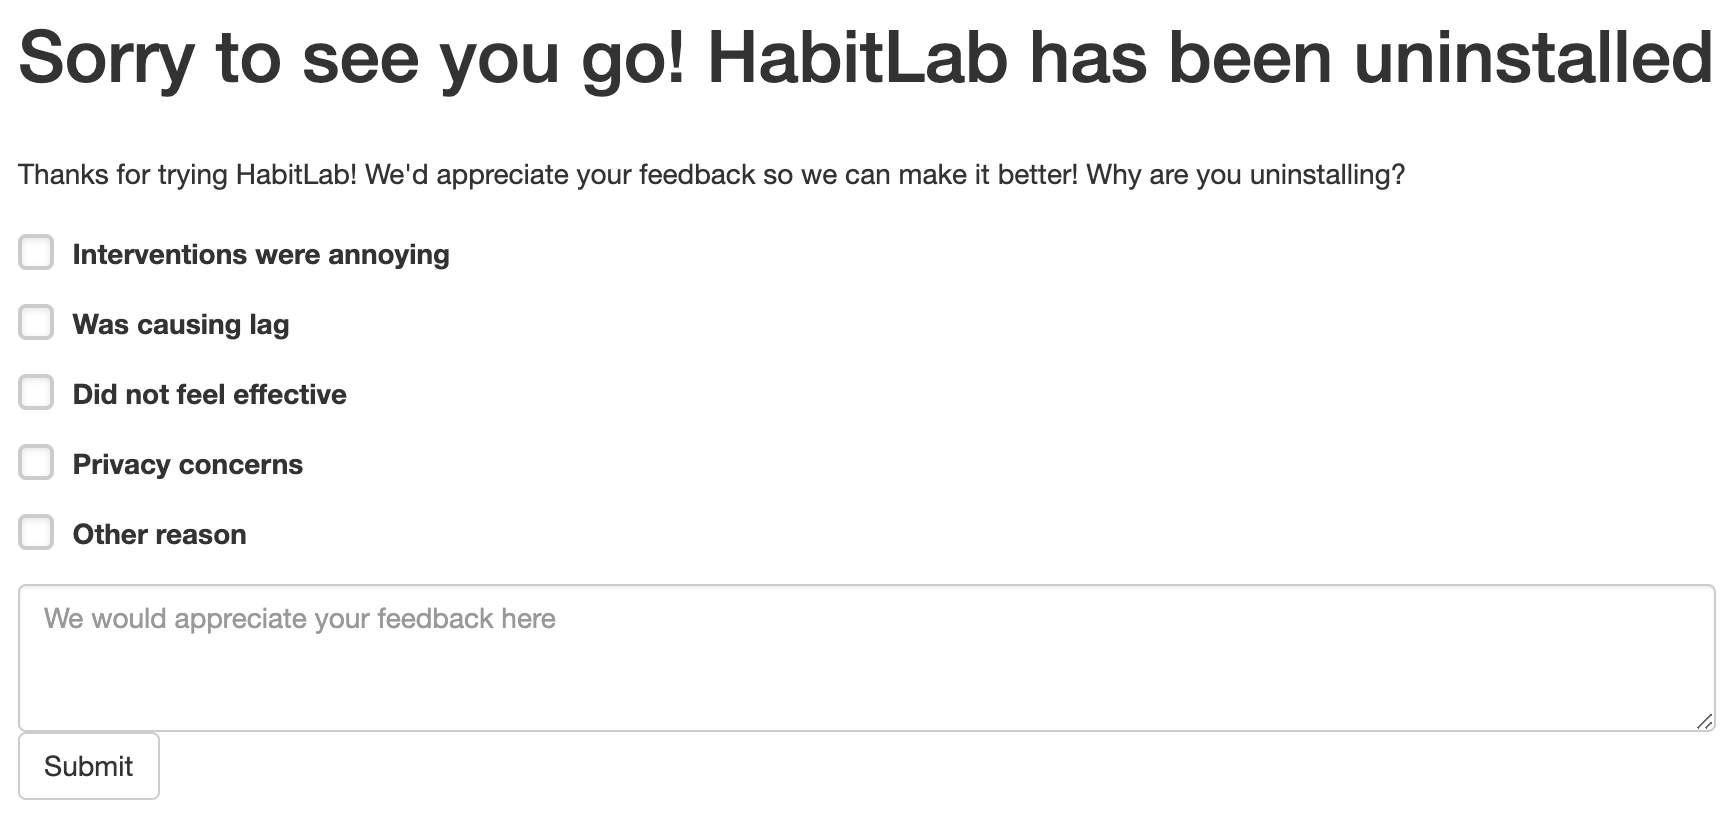
\includegraphics[width=\linewidth]{figuresS/uninstall_survey}
\caption{The survey shown to users if they uninstalled.}
  \label{fig:uninstall_survey}
\end{figure}

We asked users their reasons for uninstalling. Users could select more than one of our predetermined categories, and leave free-form feedback if their reason did not fit into any of our categories. Of a total of 4635 users who responded to our uninstallation survey, they chose 5782 reasons. A breakdown of uninstallation reasons is shown in Figure~\ref{fig:uninstall_reasons}. The most common reasons for uninstalling concerned the interventions themselves -- interventions being too annoying was the most commonly selected reason, followed by interventions being considered as ineffective. A complete list of free-form feedback users left about their reasons for uninstalling is shown in Appendix~\ref{ch:uninstall}.

\begin{figure}
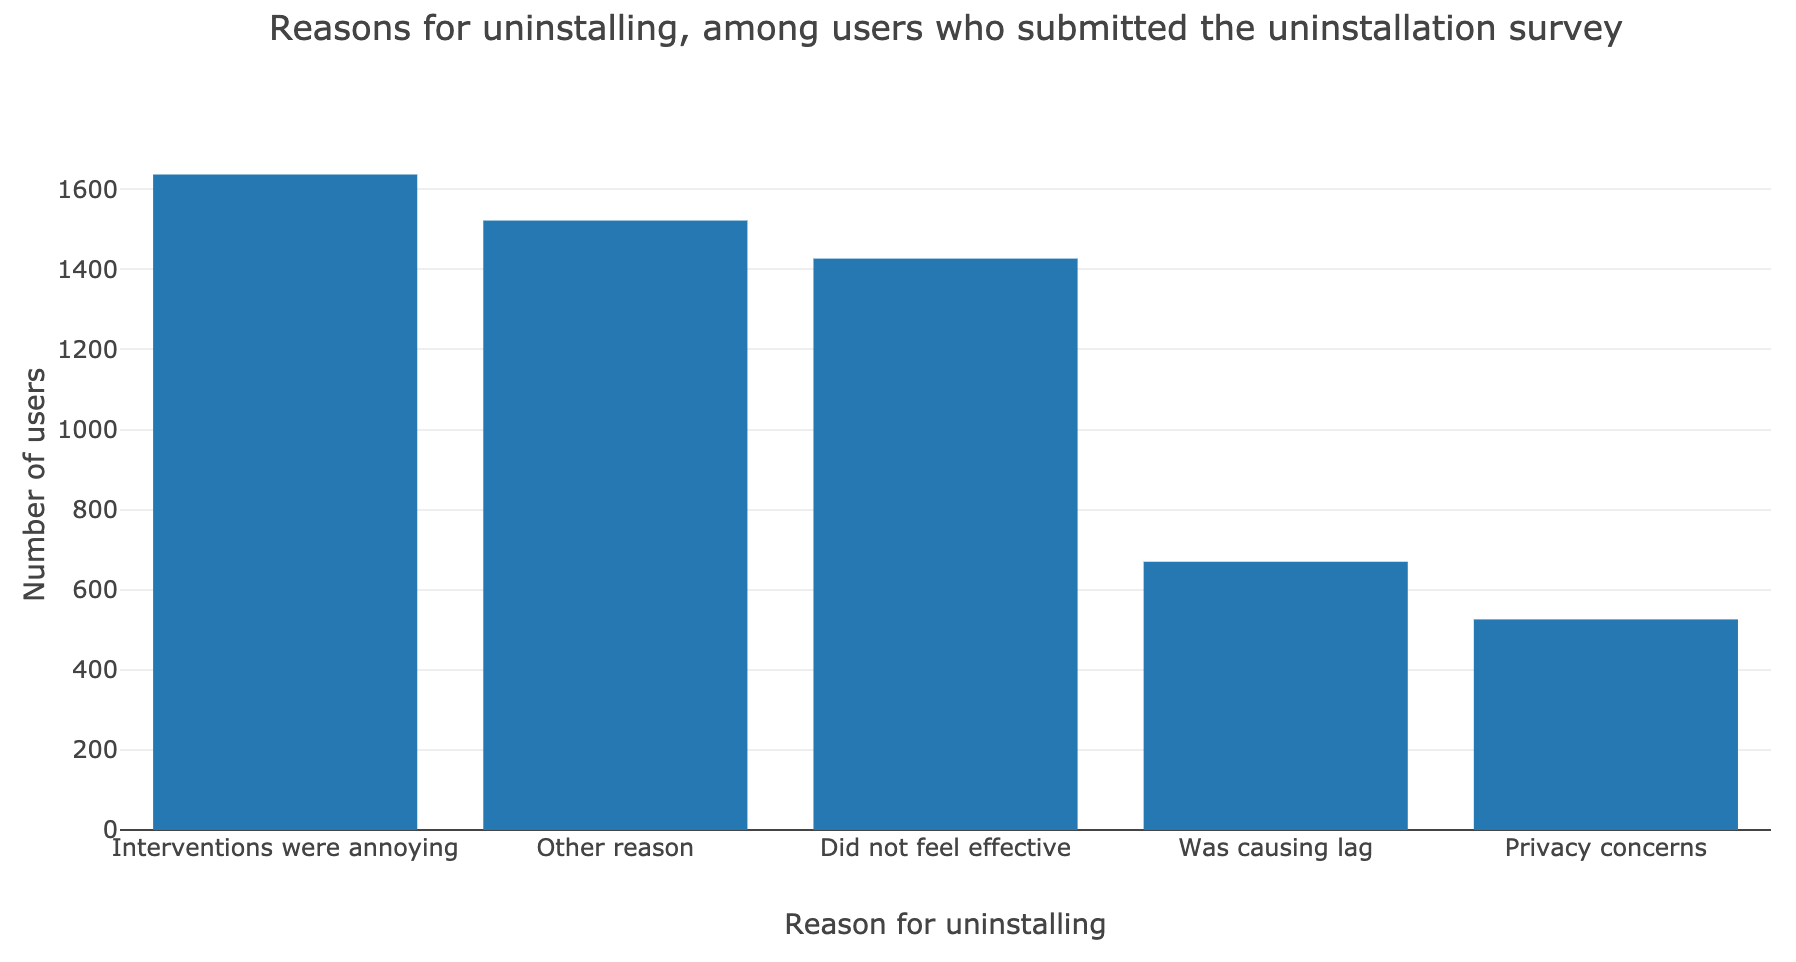
\includegraphics[width=\linewidth]{figuresS/uninstall_reasons}
\caption{Reasons users selected for uninstalling, in responses to our uninstallation survey.}
  \label{fig:uninstall_reasons}
\end{figure}



%%\section{User-Contributed Intervention Ideas}
\chapter{User-Contributed Intervention Ideas}
\label{ch:ideas}

Here is a complete list of intervention ideas that users have submitted via HabitLab:

\begin{lstlisting}[breaklines]
1: Buzzfeed:   n ,

2: Generic: "In this [x] minutes on [site name]  you would have... [fill in the gaps]

3: Generic: Disable news feed on LinkedIn, my biggest time waster

4: Amazon: Given max, if user spent money>max remind him that is useless to go to Amazon!

5: Facebook: only allow access to facebook messenger page + only allow access to Events page

6: Reddit: Just break the computer

7: Generic: motivational quotes

8: Generic: confirmation before loading the page, with a certain time forcing you to think

9: Facebook: Remind us Facebook admitted that it has always been a data mining Co. Period...

10: Youtube: Nudge after watching X minutes of video

11: Generic: before opening the site, display a (personal) list of alternative things to do

12: Generic: mom simulator: timed popups, are you using site because <x>? do <y> instead

13: Twitter: remove cats, categorized very popular BS feeds such as Only in Russia or similar

14: Generic: Automatic redirects to a more useful (user chosen?) site

15: Generic: Slow your scroll speed the longer you are on the site.

16: Netflix: Set time for length on website, after that time length, close tab.

17: Generic: Monitorize time spent on internet at all

18: Generic: Count limit number of posts, shares, reactions, etc. basically 'acts'

19: Generic: Ask when site opened if its related to goal.Limit tabs #, Use pomodore. timebox

20: Generic: Delay any temptive idea to search ask does it really make a difference in ur lif

21: Generic: http://humanetech.com/

22: Generic: I can suggest much more if if you enable me to. I have lots of ideas

23: Amazon: A budget reminder, so people don't end up overspending browsing random items.

24: Generic: stops you visiting a selected site for a while after your first visit

25: Youtube: Every minute it would display the amount of data used by youtube.

26: Generic: As I prep for tests, I'd love to get encouragement to spend time on some sites.

27: Amazon: It will tell you how much you spent and if you spend over $50, it block Amazon

28: Generic: Nudges applied to all bookmarks. e.g. to justify my visits to favourite websites

29: Generic: Generate a social media post announcing how much time you've wasted and where.

30: Generic: an hourglass of the mins I have to live, and how many of them are spent online

31: Generic: Prevent me from browsing sites during certain times.

32: Generic: Disable or limit clicks on outgoing links on a page

33: Amazon: Donate money to charity on your behalf

34: Generic: I just need a tracker for a total time spent in the internet.

35: Generic: Could you please design a tracker for a tomal time spent in the internet?

36: Generic: I would like to b abl to change the size of the "timer". Current one is too smal

37: Nytimes: Limit to two (or N) links clicked from the homepage each visit (or per hour)

38: Nytimes: Warning before loading the site for the second time in less than an hour

39: Generic: Remind me I just opened/closed the same damn tab 7m ago. For the 14th time today

40: Youtube: play asmr videos only

41: Generic: Add a blurry overlay to the screen that gets worse as time goes on.

42: Generic: For a porn website, add popup memes during the videos.

43: Facebook: Close the tab after a certain amount of time

44: Generic: Goals reminder: reminds you of your goals to promote better decisions

45: Netflix: Prompt user to confirm if they wish to continue watching before next auto play

46: Youtube: Force video to take entire window (not fullscreen, just larger theatre mode)

47: Youtube: Force disable autoplay

48: Youtube: Restrict the number of links that can be followed in one session (Wikipedia too)

49: Generic: 1 thing that u need to do & 1 thing you wish you could do if u had more time

50: Gmail: Limit the number of refreshes to inbox before auto-logging out

51: Generic: A popup reminder of why this is important to you, e.g. "your novel is waiting"

52: Generic: How about tracking time spent in Incognito mode?

53: Gmail: Self-set timer - e.g. reminder every 30 mins

54: Youtube: Reminder triggered by start of new video or pausing video

55: Facebook: Force you to wait at least 60 seconds before a finished comment is posted. PLZ.

56: Generic: Ask what your goal is for the visit

57: Generic: Ask how much time you want to spend on a site before the tab closes

58: Twitter: Make notification updates non-live - e.g. once per hour / 2 hours

59: Buzzfeed: redirect to home screen or site of choice

60: Facebook: redirect to random wiki

61: Netflix: close page at end of episode or when paused

62: Gmail: apply to-do list with task-based timer

63: Generic: Prompt for hourly pay rate.  Express time wasted in dollars wasted.

64: Generic: display total weekly stats at top of page

65: Youtube: closes when the viewer watches a certain amount of videos

66: Amazon: Do you need what you are about to go here and look for? (any eCommerce, really)

67: Generic: Restricts how many times you can open a site. eg 10-20x (For me, a stocks site)

68: Generic: 1 minute assassin, but w/o stupid "add time" button. Clicking that feels amazing

69: Twitter: limit thread or hashtag to 2o tweets

70: Custom: limit comments to 1 page , or remove next page button

71: Facebook: Meditate: count n in breaths and n out breaths (e.g. n = 3-5) before entering

72: Youtube: Prevent constantly changing videos by showing a pop up

73: Generic: sync with Google Tasks (or whatever task manager), show what is due next

74: Amazon: A counter that shows the number of clicks...the number of items you've viewed.

75: Generic: Sentences like "In the time you spend here weekly you could learn X in Y weeks"

76: Youtube: Lock the video interface and then slowly turn down the volume

77: Generic: Spanish please

78: Facebook: Only show 3 posts from the newsfeed, no more.

79: Twitter: Only show 10 tweets and don't load any additional ones when you scroll.

80: Generic: Changing end-of-day from 12am to 4am would be better for me, still up at 12am.

81: Reddit: Ask "why did you visit Reddit"? (A) Share something (B) Break. (C) etc...

82: Generic: Scroll Reseter: Automatically scroll back to top of page after N scrolls.

83: Generic: Show link to some alternative website you could be spending your time on.

84: Generic: Disables clicking for the first 15 seconds on the website.

85: Generic: Delays 15 seconds between clicking a link and having that link open.

86: Facebook: Popup msg spend time with family and friends with calc time wasted(avg life - t)

87: Generic: Solve basic math problem

88: Generic: x min assassin aggregated per some webs (x set up by user)

89: Generic: A big text saying: You have some important things to do!

90: Generic: a large message appears blocking the screen content

91: Netflix: Ask you how many episode(s) you will be watching

92: Generic: Ask me: Is this educational?

93: Facebook: Remove News Feed for a Day

94: Generic: send a warning/stop after opening x number of links

95: Generic: nothing

96: Amazon: Ask the person if they NEED the product, or just WANT the product impulsively

97: Amazon: паотьшгопимрнготьргемсавукцчяфйотбдлтнпаапмирпне

98: Reddit: Selected subreddit- Only allow access to selected subreddits for a little time

99: Youtube: Prepare for IIT JEE, see only relaxation music and iit related lecturesvideos

100: Generic: Ask how much time I want to spend on the site, close the tab after time runs out

101: Twitter: Scroll freezer

102: Generic: An exploding burst of colour & glitter with text - time to go outside & play

103: Generic: An exploding burst of colour with the text 'time to go outside & play'

104: Amazon: Show a timer in the corner that says how much time you've spent browsing

105: Amazon: Count the number of products/pages you've clicked on since visiting the site

106: Generic: What is your spending limit for this website/purchase?

107: Generic: In general: offer sign in option first for extension, handy if more than 1 pc

108: Generic: Also, increase text limit nudge suggestion :P

109: Amazon: What you want to buy? And how much do you want to spend? And inject amount  cart

110: Facebook: Blocks specific Facebook functions such as Feed and spamming notifications.

111: Youtube: stops you from being able to watch a video after watching a set amount of videos

112: Generic: Remove instagram feed

113: Facebook: Set time that you want the browser to block your Facebook.

114: Generic: A video montage of people accomplishing things to show what you're missing

115: Generic: The screen turns blank every 10 seconds with a message

116: Generic: an updated list of things you could have accomplished in the time you've spent

117: Gmail: Limit or alert after 30 seconds on a "compose" screen. Emails should be short.

118: Generic: flip the screen upside down

119: Generic: Shake the screen (window) visually or temporarily black it out

120: Generic: A animated figure pops on the screen point to there watch and taps it.

121: Calm: Do something productive

122: Gmail: Read or Go for a walk

123: Youtube: Call a Friend

124: Generic: Not a nudge, but a timer so that this only works during work hours would be fab!

125: Generic: Combine with a pomodoro timer to make this a super productivity tool

126: Generic: Holy grail> an active hours function+pomodoro, that live syncs across devices

127: Twitter: hide retweets that are trending too quickly, as they're likely time-wasters

128: Amazon: Ask what I am specifically shopping for

129: Generic: darken screen; large timer in center. press "space" to leave; ESC to stay

130: Generic: Please make this for Firefox

131: Twitter: Put fake tweets into feed asking with increasing frequency, "Why are you on Tw?"

132: Youtube: videos play faster, or ads play slower, gets progressively worse

133: Generic: freeze keyboard controls until the tab is removed after a set period of time

134: Facebook: Ask you a group of peoples feed to show only (eg: just family)

135: Generic: 5 minute assassin option(similar to the 1-minute assassin nudge)

136: Generic: multi nudges at the same time

137: Generic: 5 minute assassin timer nudge(similar to the 1 minute assassin nudge)& show time

138: Generic: When I am getting off track from the original reason I went online. Surf time

139: Generic: Flip the screen vertical

140: Amazon: Logs you out after a set amount of time.

141: Generic: ask how scrolls I need to do to block it

142: Gmail: sticky note pop out on your screen and say girl or boy you have 5 mins left

143: Twitter: Pop up that says, "Haven't you already read this?" (News services, too!)

144: Facebook: Simple questions: Did you find what you were looking for? Still here? etc.

145: Generic: Plays an alarm sound every x minutes, for example every 10 minutes you hear it.

146: Youtube: show time spent on youtube

147: Youtube: que no pongan anuncios en pleno video(en medio) del video

148: Youtube: stop auto-play of next video - replace with a prompt/timer/reminder if possible

149: Amazon: ask what online to buy, how much time needed, then prompt when approaching time

150: Generic: Telegram

151: Youtube: Close after 1 hours

152: Youtube: Only show the videos you need

153: Generic: Timer but flashes every X seconds in diff parts of screen

154: Generic: if you visited a website for the 20iest time in the last 3 hours, block it

155: Generic: blank screen intermittant after said time

156: Generic: feedeater& thinktwice (bcz user get there with purpose, but feed wastes) quora,

157: Youtube: Block the tab at certain times that you can set up

158: Youtube: Is this for study or not ?

159: Youtube: Auto-pause a video after a certain amount of time and show your stats.

160: Generic: Pop ups every 5 minutes that remind you and ask if you should still be on there.

161: Generic: pictures to a meme or to a set picture which motivates people,like family pictur

162: Youtube: Receive a warning after spending some specified amount of time

163: Generic: Every min, flash screen off for 5 seconds and remind them their goals + accompl.

164: Youtube: At a certain time, set by the user, the video will start stutter.

165: Youtube: Classify the video title(fun/usefu) notifies user if he/she spents too much time

166: Generic: Make the remind/aim banner dark instead of white

167: Generic: Ability to set specific nudges on or off, I just like certain ones more.

168: Generic: Allow control of consumption by amount of data spent

169: Generic: For all websites, ask how long you want to be on the internet for all together

170: Youtube: Detect "Recommended" browsing and how many videos you've hoped on a row

171: Youtube: Click (twice or let users wait) to show the video recommendations on the side

172: Facebook: Ask math question before opening site.

173: Generic: Linkedin


174: Youtube: Get rid of sidebar

175: Twitter: For a certain time frame, have only a certain subset of tweets appear on feed.

176: Twitter: Tick down the # of links, replies, etc. you click on then freeze for some time.

177: Facebook: Hide repeteated posts or hide posts that has been already displayed

178: Generic: Ask to stop or close tab

179: Generic: Higher Self. Display a prompt encouraging user to reflect on values

180: Generic: Link Lock: Sets (x) amount of links/videos user can click per day per site

181: Generic: The time wizard, but non-intrusive. The Mission Objective, but on specific sites

182: Youtube: Vomiting audio

183: Generic: Vote if tab "created idea" or "killed time" on close; report ideas by tab title

184: Facebook: I want the few second delay just for facebook

185: Generic: A notification to bring user back to the browser and stop surfing offline files

186: Generic: Go to bed (with insomnia option)

187: Amazon: Asks you what you are here to purchase

188: Reddit: Shows only the top 10 threads in the 'popular' section

189: Facebook: hide news feed

190: Generic: Personalized messages on screen (ex. "Don't you want to go to medical school??")

191: Generic: Change all images to Nicolas Cage face (Like chome's ncage extension)

192: Generic: every minute, the webpage becomes gradually more pixelated

193: Generic: Put links into a „TODO”-like list instead of opening them. This helps focusing.

194: Generic: After a configurable amount of time, close website and don't let me reopen it.

195: Generic: „Lock to this page”
Helps focusing on learning material. Block other pages.

196: Youtube: Limited amount of videos one can watc, as sometimes you need to watch for work.

197: Youtube: Block certain channels

198: Reddit: Remove the "next page" link on the old reddit, or block auto-scrolling on new

199: Reddit: Ask how many minutes to keep the tab open before killing it

200: Generic: pixels start getting blacked out

201: Reddit: Show only the first page of each subreddit and hide (or show less)

202: Generic: Time limit for a group of websites eg 10mins all social media, then no access

203: Buzzfeed: for them to stop being feminists

204: Ted: stop

205: Duolingo: learn spanish or die

206: Facebook: hello fellow white mothers

207: Facebook: HabitLab could post amount of time spent and visit count on FB wall

208: Generic: Progress bar that moves forward as user is productive and backward when not

209: Youtube: Turn off the sound for youtube/Pause the video, or put the video in slow motion

210: Youtube: Pauses the video and reminds you of a previously set reminder.

211: Youtube: Make a list for how much time you want to spend on each site and be reminded

212: Netflix: Shows you how many hours you have wasted on that particular show

213: Netflix: Close tab after preselected numer of episodes watched

214: Netflix: Lock episodes for series to one per day

215: Generic: Break time - set your timer for your break between tasks

216: Amazon: Shows your monthly/weekly/yearly purchase history dollar amount $$$.

217: Amazon: Removes Buy buttons, replaces them with Add to List so you have to wait & think

218: Youtube: Ask to minimize tab, so user can just listen not watch (for music or talks)

219: Buzzfeed: Tells you that you have better things to do and after that close after 60 second

220: Generic: Ask how are you feeling right now? or Is there a task you are avoiding?

221: Generic: Could you use a break - get up and take a walk.

222: Generic: Turns the entire screen white gives you a life quote and asks to continue

223: Twitter: Show only your notifications; clicking on any links force-closes Twitter.

224: Generic: Switch to 1st tab in browser window after specified time.

225: Generic: Mindfulness popup, after specific time elapsed.

226: Generic: After a certain amount of time, asks what your purpose is for still being there

227: Generic: make it black and white

228: Twitter: Don't allow feed refreshes

229: Twitter: Set a max time allowed per day, week, month

230: Youtube: When a video finishes Can you remove suggestions or next video?Or even playlists

231: Generic: A pomodoro technique complement. Work 20' and get your 5' treat.

232: Youtube: Close after a certain amount of time and restrict access until you say

233: Youtube: mode music please

234: Youtube: mode music please

235: Gmail: (if enabled) remove the "new messages" icon from social and promotions tab

236: Duolingo: Mejor es aprender otro idioma

237: Duolingo: aprender

238: Youtube: Ask me before what type of videos I want to watch/block and work over this list

239: Generic: PowerUSE: Utility-Span-Expiry. State purpose, make estimate, agree hardstop end.

240: Youtube: Music only mode. Disable videos, but allow music. To listen while working.

241: Facebook: Include Facebook Messenger (www.messenger.com) blocking messages or a time limit

242: Generic: advertising videos goggle up my RAM, slowing my page loading. Stop them please.

243: Generic: Top-level comments only. Removes all reply comments.

244: Generic: Block access to the website for a period of time

245: Netflix: Remove Suggested Shows/Movies

246: Twitter: Remove Likes/RT for your Tweets and removes comments for other people's Tweets

247: Youtube: Hide the comment section. A total time-killer.

248: Generic: Mood Tracker

249: Generic: Describe mood before clicking on a website

250: Generic: If on a website for too long, play a recording of yourself saying other ideas

251: Generic: A reminder that the work won't disappear, but these other distractions can wait.

252: Youtube: Only show the top 5 comments (and 3 replies per comment).
\end{lstlisting}


\section{Discussion}

%\msb{Would love to see a page of Discussion in this chapter. Possible topics include: (1) Do you think the same design principles would allow a research system to succeed in other domains? If so, why? If not, why not? (2) What did we try that didn't work, and why? (3) Of the stuff that you did in designing HabitLab, what do you think is the most central novel idea?} \geza{done}

The HabitLab system was built on the premise that experimentation for behavior change can be useful for both end users as well as researchers. Based on our experiences building, growing, and receiving feedback on the system, we have reasons to believe that this premise is true in certain respects, while false in others. Specifically, certain types of experimentation can be well-aligned with end user goals and perhaps even enhance the user experience, but other types of experimentation may be detrimental to the user experience.

We observed that among negative feedback we received for the system, the most common complaint related to experience sampling -- users simply did not like being forced to answer questions, regardless of how minimally intrusive they were. The next most common complaints were necessary artifacts of our experimentation and A/B testing -- some users wanted more control over the frequency of interventions and which interventions were seen at particular times, but we wanted to randomize these as part of our experiments. We also often found that users requested additional customizations that would provide them with more control over interventions, but were reluctant to implement them as they would complicate experimentation by making it more difficult to quantify intervention effectiveness.

We also find that users may be unsatisfied with ``baseline'' or ``control'' conditions in an in-the-wild context. Specifically, some of our experiments necessitated that users occasionally not be shown any intervention on a particular visit, so that we can observe baseline time spent in the absence of an intervention. However, whenever we had such an experiment running, this resulted in a flurry of user complaints that interventions were not working. Even when users were aware of this, or were aware of the rotating nature of interventions, they expressed dissatisfaction that they were not able to see particular interventions each visit. Thus, this is a clear example of researchers' needs for experimentation being in conflict with users' preferences.

That said, several forms of experimentation did not conflict much with user expectations. In contrast to experience sampling, which resulted in both user complaints and increased attrition, we found that adding the same question as a one-time onboarding question did not result in user complaints or increased attrition. Likewise, while we found that the intervention rotation strategy increased attrition and resulted in some user complaints, it also increased intervention effectiveness.

Thus, while we would optimally always be able to find experiments which both satisfy scientific needs as well as preferences of end users, they are often in conflict. In-the-wild experimentation platforms such as HabitLab must sometimes make compromises between these goals. With HabitLab, our approach to navigating this problem has tended to be experimental. Specifically, we A/B test our experiments and constantly monitor user feedback and attrition rates in experimental conditions compared to baselines which we know to have good user satisfaction. If a particular experiment is causing a large increase in attrition, or users are unsatisfied, we attempt to modify the experiment design so we can answer the same research questions with less increase in attrition. For instance, since we found that our original experience sampling prompt design causes an increase in attrition, we A/B tested several different variations to try to find alternative designs which would collect similar data while causing less attrition.

Our general approach to this experimentation-vs-user-experience tradeoff with HabitLab can thus be described as using A/B testing so we can understand the tradeoff we are making, and looking for alternative experiment designs that satisfy our scientific goals with better user experience if they are in conflict. We believe that designers of in-the-wild experiment platforms must always be thinking about user experience, retention, and satisfaction, and cannot sacrifice these for the sake of running an experiment -- after all, an in-the-wild experiment platform's most precious asset is its userbase, and if there are no users, we cannot run any experiments.




%\chapter{Rotating Online Behavior Change Interventions Increases Effectiveness But Also Increases Attrition}
\chapter{Rotating Online Behavior Change Interventions}

\section{Introduction}

Behavior change systems today suffer from declining effectiveness as novelty wears off over time. Typically, behavior change systems utilize a \textit{static} design, which never changes. For example, to manage social media browsing time, the three popular options are to block tempting sites~\cite{stayfocusd}, use a work timer~\cite{focusbooster}, and audit time spent~\cite{khovanskaya2013everybody,rescuetimeapp}. However, static interventions suffer from high attrition and abandonment rates~\cite{collins2014social,eysenbach2005law}, and interventions decline in effectiveness over time~\cite{krebs2010meta}. Habituation eventually drives users to stop paying attention to, or avoid, static interventions---an effect often seen on the web as banner blindness~\cite{benway1998banner}. The end result is that many behavior change systems are tuned out by users, and are unsuccessful at their goals.

If static interventions are tuned out, \textit{rotation} might provide a remedy. Much like a human coach or tutor rotates between different approaches over time, rotation might maintain attention in ways that static interventions cannot. Online behavior change tools could apply similar techniques, for example injecting a visible stopwatch timer into the page on one visit to Facebook, and hiding comments on the next visit.
Techniques that personalize interventions via multi-armed bandits show positive treatment effects, suggesting that the approach may hold promise, but this existing work cannot separate the effects of personalization from the effects of rotation~\cite{rabbi2015automated, lei2017actor, paredes2014poptherapy}. %Techniques that rotate between different interventions, selected randomly or via algorithms such as multi-armed bandits, improve overall effectiveness in health intervention contexts. 
Because rotated interventions continually change the user interface, however, they may frustrate users by violating consistency and a sense of user control, leading to lower effectiveness or higher attrition. %\rak{Has this (that rotating interventions frustrate users) been measured or is this a hypothesis?}

This paper takes up the question: are static or rotated interventions more effective for behavior change? Is it possible to understand the effects of rotation in order to design more effective behavior change systems? We focus specifically on helping users who want to manage their time on social media websites such as Facebook, YouTube, Reddit, and Twitter. We perform a series of field experiments with people who sought out and installed a browser extension that we developed for online behavior change. % \rak{Maybe state why you choose these platforms? Are these sites that people spend a lot of time on? Or are they sites that people usually pick add interventions to?}

Our platform, \textit{HabitLab} (\url{https://habitlab.stanford.edu}) is a Chrome extension that features a number of online productivity interventions to help users reduce their time spent on sites such as Facebook. We released HabitLab publicly on the Chrome web store, where it has attracted over 8,000 daily active users. This user base allows us to observe real-world usage and attrition patterns over time. % real-world realistic,

We ran three in-the-wild studies on users who newly installed HabitLab. In Study 1, we compared static interventions to rotation. %Conditions rotated interventions with each new session, or every one, three, five, or seven days. 
We measured effectiveness through time on the user's targeted site, and we measured attrition by tracking when users stopped using the extension.
Results indicate that rotation is a double-edged sword. %Static interventions declined in effectiveness over time, with an estimated 5.9\% daily increase in time spent over our experiment. 
Rotating interventions reduced time spent on sites by $34\%$ per day, but at the cost of nearly doubling attrition levels.  %A follow-up correlational analysis suggests that rotation attrition was less likely when users chose their interventions themselves during installation, suggesting that these users either had a better mental model of the rotation to come, or that user control plays an important role.

% \jingyi{you don't say how long study 1 was for}
Study 2 replicates the first experiment over a longer period of seventy days, and additionally tests whether the number of interventions included in the rotation impacts attrition. The results successfully replicated the original results over a longer 70-day period, and suggested that the larger the set of interventions, the higher the probability of attrition.

% \rak{You said that this number was 50\% in the intro. Make them consistent.}
To investigate the underlying causes of attrition and mitigate the effects of rotation on attrition, we analyzed user feedback and developed a pair of interface techniques to improve the user experience in the presence of rotation, which we deployed in Study 3. The first technique is informational, aiding people's mental models by reminding them that the system may show a different intervention on each visit. The second technique focuses on user control, providing the same information as well as a just-in-time mechanism for people to opt out of each new intervention as they see it. Results indicated that these interventions reduced attrition by over half, so that $80\%$ of new users were still using the system actively after a week.

% \jingyi{``and others'' vague}
In sum, this paper contributes the first comparison of static and rotation intervention strategies in behavior change, a living laboratory system that allows us to deploy this investigation and other field experiments, and interaction design strategies that can help offset increased attrition due to rotation. Its results suggest that people may be more able to control their social media usage more effectively than using today's common techniques such as site blockers. The rest of the paper is organized as follows: we first review studies of behavior change to develop our research question and hypotheses; we then describe our studies and results; we close with reflections and future design directions.







\begin{comment}
Excessive recreational online activity, or ``cyberslacking'' is a major problem. Hence, numerous productivity interventions, such as time trackers and site blockers, have emerged to help users reduce their time online. Existing productivity tools typically always show the same intervention; however, techniques that alternate between different interventions (selected via algorithms such as multi-armed bandits) have been found to improve overall effectiveness in various health intervention contexts. This can be applied to online productivity tools as well -- i.e., hiding the news feed on one visit, injecting a timer into the page on others, etc.

Alternating interventions has typically been done in the context of an adaptive intervention selection algorithm (e.g. multi-armed bandits), and the benefits have been attributed to personalization -- certain interventions are more effective for certain individuals, and by exploring which interventions are most effective for the individual, the algorithm can maximize effectiveness in the long run. 

However, we believe that our understanding of the effects of alternating interventions may be incomplete. Certain health interventions have been found to decline in effectiveness over time, and banner blindness is a well-known phenomenon in online advertising -- if users analogously develop blindness to interventions, could the novelty brought by alternating interventions itself improve effectiveness, by preventing the user from developing intervention blindness? Such effects are important, because declines in intervention effectiveness over time violates a major assumption of multi-armed bandit algorithms -- that the rewards, e.g. the effectiveness of the interventions -- do not change over time. If alternating interventions has a significant positive effect on effectiveness, intervention selection algorithms need to take this into account.

% https://www.sciencedirect.com/science/article/pii/S0091743510002318

Alternatively, alternating interventions can have negative effects -- users may be annoyed and fatigued if they constantly see different interventions, as it may violate expectations of a consistent user experience. Users may also feel a lack of control if the system is choosing which interventions to show them, rather than always showing the same one. If a user particularly dislikes one of the interventions, the user may be exposed to it while the system is exploring the space of interventions, which risks causing user dissatisfaction. These factors may lead to alternating interventions contributing to increased rates of attrition -- which intervention selection algorithms need to take into account.

To answer these questions of in which ways alternating interventions can be beneficial or harmful, we developed a Chrome extension, HabitLab, that features a number of online productivity interventions to help users reduce their time spent on sites like Facebook. We released it publicly on the Chrome web store, and ran a pair of in-the-wild studies on users who newly installed the extension, where we varied how much we were alternating between interventions. Users were unpaid, organic installs from the Chrome web store rather than artificially recruited participants, which allows us to better observe real-world usage and attrition patterns. We found the following results:

\begin{enumerate}
\item Users who are constantly rotating between interventions have higher rates of attrition than users who consistently see the same intervention.
\item Interventions decline in effectiveness over time
\item Interventions are more effective at reducing users' time spent when they are shown alternating between different interventions
\item Users are less likely to attrition if they chose their interventions themselves during the onboarding process
\end{enumerate}

These results led us to hypothesize that the increase in attrition observed due to alternating interventions may be a result of violation of user expectations (due to users having an incorrect mental model), or users feeling a lack of control.

To investigate the underlying cause and mitigate this attrition, we developed a pair of interface techniques shown when a new intervention is seen for the first time. The first interface just repeats information (that users saw during onboarding but may not have read) that the system may show a different intervention on each visit, while the second interface gives users a sense of control by allowing them to opt-out of seeing the intervention in the future. We found that adding these interventions both significantly decrease attrition (fake result).

\end{comment}

%These results led us to propose a new UI technique that retains the benefits of alternating interventions, while reducing the negative effects on attrition. Whenever

%These results lead us to suggest new algorithmic and UI techniques for behavior change interventions that allow us to exploit the benefits of techniques that alternate between interventions, while avoiding the negative effects on attrition.

% Algorithmic techniques we propose to limit attrition caused by alternating between interventions are 1) limit the exploration speed such that the user is not overwhelmed by the rate at which they are seeing new interventions, and 2) model individual interventions' likelihood of causing attrition so that the algorithm is less likely to show interventions which are likely to cause attrition.

% UI techniques we propose to give users a sense of control and reduce violation of expectations caused by the system randomly introducing new interventions are 1) explicitly show users when a new intervention is going to be introduced with an option to opt-out of seeing it, and 2) make the schedule at which new interventions are introduced predictable and known to the user.

% However, online productivity tools operate on a different timescale 

% The traditional narrative on multi-armed bandits has been that they provide benefits via personalization -- certain interventions are more effective for certain individuals, and by exploring which interventions are most effective 



%People spend a lot of time online

%Productivity interventions try to reduce their time online

%There are techniques that make use of an ensemble of interventions, that can outperform just using a single intervention, for example multi-armed bandits

% However we suspect that users develop blindness to interventions over time, hence we wished to investigate whether novelty effects exist and to quantify their magnitude.

% Novelty effects are important, because declines in intervention effectiveness over time violates the assumptions of multi-armed bandit algorithms.

% We investigated this in the context of a system we developed, HabitLab, which is a Chrome extension that features a . It is published on the Chrome store and can be used by anybody, and currently has over 4000 daily active users.

% We found that 



%----------------------------
% RQ
\section{Behavior Change And Motivation}
The field of persuasive technology studies how technology can be used to influence behavior~\cite{fogg2002persuasive}. Persuasive technology systems have been successful in promoting behaviors such as sustainable resource usage~\cite{froehlich2009ubigreen}, fitness~\cite{consolvo2008activity}, sleep~\cite{kay2012lullaby,choe2011opportunities}, healthy eating~\cite{noronha2011platemate,epstein2016crumbs}, stress management~\cite{adams2014towards,sanches2010mind}, smoking cessation~\cite{paay2015personal}, and productivity~\cite{whittaker2016don, kim2016timeaware}. One common framework of behavior change is the B=MAT model~\cite{fogg2002persuasive}, which states that desired behaviors result when motivation, ability, and a trigger (a call to action) are all present. Another framework of habit change is the habit loop~\cite{eyal2014hooked}, which tells us that designs can build habits via a repeated process of displaying a trigger, having the user take an action, providing a reward, and having the user invest in the system.

A number of taxonomies characterize the design space of interventions, both general~\cite{michie2013behavior, behaviourchangewheel, abraham2008taxonomy, dolanmindspace} and domain-specific~\cite{hardeman2000interventions, west2010behavior}. Michie's behavior change taxonomy lists 93 techniques for behavior change, clustered according to the cognitive phenomenon they target~\cite{michie2013behavior}. Systems have investigated effects of these techniques individually, such as using ``cheating'' to support lapse management~\cite{agapie2016staying}, using different framings to present results~\cite{kim2016timeaware}, or setting goals and plans~\cite{agapie2016plansourcing}.

% One of the most comprehensive investigations we
% identified is a recent meta-analysis of 85 studies by
% Webb et al. (2010) that found interventions that were
% strongly based in theory had greater impact than those
% that were not, and interventions that incorporated more
% behavior change techniques tended to have larger
% effects than interventions that incorporated fewer techniques

% Within the CSCW community, behavior change has been an active area of research. One major topic inspiring our work is users' desires to curb or control their time spent on social media sites. People pressure themselves to, and often do, make efforts to reduce their time spent on social media sites such as Facebook and Twitter~\cite{Sleeper:2015:ILI:2675133.2675193,schoenebeck2014giving}. This paper builds on this literature, contributing studies of how people might become more effective at this goal. Sociotechnical systems are also locations where people discuss behavior change~\cite{chancellornorms}, and find social support~\cite{Ko:2015:NGI:2675133.2675244, Chung:2017:PTB:3025453.3025747}. Behavior change often requires self-tracking, self-experimentation, and personal informatics~\cite{Karkar:2017:TFS:3025453.3025480}, leading to opportunities to share data and progress with trusted others~\cite{Chung:2016:BNA:2818048.2819926, pina2017personal}.

\rev{People use a variety of sociotechnical systems to support behavior change, including forums~\cite{eysenbach2004health, chancellornorms}, social sharing~\cite{poirier2012social, Chung:2016:BNA:2818048.2819926, pina2017personal, Ko:2015:NGI:2675133.2675244}, personal informatics~\cite{li2010stage, Chung:2017:PTB:3025453.3025747}, and self-experimentation~\cite{Karkar:2017:TFS:3025453.3025480}. People use behavior change forums to gain social support~\cite{hong2012outcomes} -- meeting social needs such as approval and esteem~\cite{kaplan1977social}. They do so by providing users with information and advice~\cite{hong2012outcomes}, and establishing norms~\cite{chancellornorms}. They also facilitate social comparisons~\cite{davison2000talks} which influence behaviors, as social comparison theory states that users seek to bring their behaviors in line with norms~\cite{festinger1954theory}. Communities also help users find others with similar experiences~\cite{huh2014health} who can help them through the process of recovering and adapting to changes~\cite{newman2011s}. Social sharing~\cite{poirier2012social, richardson2010online} works by helping users receive support through social interactions, and encouraging accountability~\cite{epstein2015nobody}. Personal informatics support behavior change through stages of preparation, collection, integration, reflection, and action~\cite{li2010stage}. The theory of lived informatics~\cite{epstein2015lived} adds additional stages where users choose tracking tools, and alternate between lapsing and resuming their tracking behaviors. HabitLab combines personal informatics and self-experimentation to support behavior change. Our study draws on lived informatics by evaluating whether rotating interventions is an effective strategy to combat lapses such as ignoring interventions or uninstalling.}

% Of course, sociotechnical systems may also have deleterious effects --- communities may set unhealthy norms such as encouraging eating disorders~\cite{chancellornorms}, and social sharing can cause anxiety~\cite{munson2010happier}, impression management concerns~\cite{consolvo2014designing}, and make users unwilling to set goals~\cite{munson2015effects}.

% \msb{Can you pull this together into a summary of what we draw from this literature and how it influences HabitLab or our study?}

\rev{One major topic inspiring our work is users' desires to curb or control their time spent on social media sites. People pressure themselves to, and often do, make efforts to reduce their time spent on social media sites such as Facebook and Twitter~\cite{Sleeper:2015:ILI:2675133.2675193,schoenebeck2014giving}. Yet this is difficult because users turn to social media to address their need to belong, the need for self-presentation, the need for self-esteem~\cite{nadkarni2012people}, the need for entertainment and gratification ~\cite{raacke2008myspace}, and self-affirmation ~\cite{toma2013self}. Whether social media use improves well-being is a complex question depending on the nature of the engagement ~\cite{uysal2013mediating, marche2012facebook, lin2015emotional, kim2011facebook, muise2009more, sagioglou2014facebook, tandoc2015facebook}, but thanks to instant gratification and sites' use of gamification~\cite{chou2015actionable, zichermann2011gamification, huotari2012defining} and behavior design techniques~\cite{fogg2002persuasive, eyal2014hooked} to drive engagement, users keep coming back to the point that some consider it an addiction~\cite{andreassen2012development, ryan2014uses, tang2016personality, turel2014examination}.} %Furthermore, social media sites make heavy use of gamification to drive engagement on their sites~\cite{chou2015actionable, zichermann2011gamification, huotari2012defining}, and are cited as successful applications of behavior change theories~\cite{fogg2002persuasive, eyal2014hooked}.} %Furthermore, social media sites are designed to maximize user engagement, with features closely following gamification strategies~\cite{chou2015actionable} and behavior change theories~\cite{fogg2002persuasive, eyal2014hooked}.}

% datu2012does

% Social media is particularly addictive be

% \rev{expanded the related work discussion on sociotechnical theories. list the theories driving these papers. social support cscw theories. why people use forums for behavior change support what role do other people play in driving your behavior change. collective exercise. why are social media particularly hard to manage your behavior with why is social media addictive.}

% \rev{festinger's social comparison theory postulated that social behaviors could be predicted largely on the basis of the assumption that individuals seek to have and maintain a sense of normalcy and accuracy about the world}

% http://journals.sagepub.com/doi/pdf/10.1177/1524839911405850
% Harnessing Social Media for Health Promotion and Behavior Change

% \rev{Communities and collaborative support can help achieve behavior change goals. }

Much previous work has focused on gamification as an approach to design behavior change systems~\cite{deterding2011game}. Gamification has been shown to have positive effects on engagement and outcomes in behavior-change contexts such as promoting healthy habits~\cite{cugelman2013gamification, lyons2014behavior} and improving  educational engagement~\cite{anderson2013steering, anderson2014engaging}, though effectiveness varies depending on the context and design~\cite{6758978}. % Popular online services such as Facebook and LinkedIn make heavy use of gamification to drive engagement on their sites~\cite{chou2015actionable, zichermann2011gamification, huotari2012defining}.

Attrition is a major challenge in behavior change systems. Attrition~\cite{eysenbach2005law}, also known as dropout, occurs when participants stop participating, leave, or uninstall the system. Persuasive systems built for weight control and therapy have shown substantial attrition rates in longitudinal studies~\cite{Bernier1986,paredes2014poptherapy}, and prior work in CSCW has sought to help reduce attrition rates through techniques drawn from dieting and addiction research~\cite{agapie2016staying}. % This paper contributes a direct study of attrition and its antecedents.%this study the increments in attrition has not been discussed in detail or quantified in the context of rotating interventions in behavior change systems.

A recent trend in behavior change systems has been the concept of personalizing interventions. Such systems explore several possible strategies using techniques such as multi-armed bandits to find the intervention that is most effective for the user~\cite{paredes2014poptherapy, rabbi2014automated}. For example, PopTherapy demonstrated personalized messaging could be found through such techniques~\cite{paredes2014poptherapy}. Likewise, HeartSteps conducted tens or hundreds of micro-randomized trials on users~\cite{doi:10.1111/j.1740-9713.2015.00863.x}.  When multi-armed bandits are just beginning to get feedback from a user, they will try out several different interventions to see what works. This exploration has the effect of rotation, but the amount of rotation declines as the bandit begins to personalize. In this paper, we examine the contrarian assertion that perhaps rotation should be maintained to sustain novelty even after the multi-armed bandit is aware of which intervention is most effective for the user.

% The challenges of static interventions, and the rising wave of personalization systems, call into focus: would a rotation strategy work? Or is it a weak palliative with little discernible effect? This led to our research question:

\begin{resques}[RQ]
Can a strategy of rotating interventions produce more effective behavior change systems?
%Does rotating interventions is helpful in increasing effectiveness and lowering attrition in online behavior changes systems?}
\end{resques}

%----------------------------
% HYP
\section{Rotating Interventions}
In this section, we review literature in behavior change systems and psychology to develop specific testable predictions regarding the research question.% Few studies has touched upon the quantification of effectiveness and attrition in the literature of online behavior changes systems. However, there are studies in behavior changes systems investigating the effectiveness of algorithmic interventions system. Meanwhile, previous work in behavior-change contexts has shown the porblem of attrition of behavioral interventions. This section presents a review of such studies and the proposal of our research hypotheses. 

% \jingyi{reviewed papers? i would just say past work}
\subsection{Effectiveness over time}
While behavior change systems can be effective~\cite{doi:10.1080/15228830802094429, Cuijpers2008, info:doi/10.2196/jmir.1376}, many review papers are more restrained in whether behavior change systems remain effective over long periods of time~\cite{doi:10.1111/j.1467-789X.2009.00646.x, 10.1371/journal.pmed.1000387, NORMAN2007336, 10.1007/978-3-319-07127-5_11}. The critique holds that behavior changes are long, complex processes, and the effectiveness of a system is hard to maintain indefinitely~\cite{prochaska1997transtheoretical}. Prior work suggests that the effectiveness of showing a static intervention cannot be maintained indefinitely~\cite{Hiniker:2016:MDE:2858036.2858403, riekert2013handbook}. For example, when a health behavior change system started sending email reminders, the first reminder was successful 28\% of the time, but by the fifth reminder it was successful only 18\% of the time~\cite{kaptein2015personalizing}. 

A further meta-analysis of 88 computer-tailored interventions for health behavior change suggested that the efficacy of interventions decreases over time~\cite{krebs2010meta}. This prompts our first hypothesis: %These literatures prompt our first hypothesis:

\begin{hyp}[H\ref*{hyp:decreaseovertime}] \label{hyp:decreaseovertime}
Static interventions will suffer from decreased effectiveness over time.
\end{hyp}

\subsection{The impact of rotation}
Novelty can be a driving factor for effectiveness. %Novelty has been studied for years in psychology and brain sciences. 
One study showed that novelty can influence encoding of information into long-term memory, which, in turn, may raise awareness of behavioral changes~\cite{doi:10.1111/j.1467-9450.2005.00443.x}. Studies of gamification also explore the effect of novelty on user engagement~\cite{6758978}.  %Studies of gamification also explore the effect of novelty in supporting user engagement~\cite{6758978}. 

In web design, people begin ignoring parts of the screen that have little information scent, such as ads. This phenomenon is termed banner blindness, after the commonness of the effect in internet banner advertising~\cite{benway1998banner}. As static interventions remain deployed, they may suffer from the same banner blindness and lack of novelty (wear-out) effects, suggesting a potential mechanism for the decreased effectiveness over time.

Rotating interventions may counter these effects.
Different interventions appear in different parts of the interface, making it less likely that the user would ignore them wholesale.
%In the system with static interventions, the wear-out effect may be one mechanism behind the decrement of effectiveness over time. On the other hand, 
Online behavior change systems that use machine learning algorithms such as multi-armed bandits hone in on a small number of interventions to use~\cite{paredes2014poptherapy, rabbi2014automated}, but during the early exploration phases they are essentially rotating between interventions. %Evidence shows that behavior changes system which implemented the algorithm showed higher effectiveness in the short term~\cite{paredes2014poptherapy}. 
%Rotating between interventions without machine learning systems behind the scenes also has proven effective in PMS system. Comparing to PMS system that shows static intervention, 
Systems that personalize interventions~\cite{kaptein2015personalizing} or deploy many micro-studies% Additionally, one study that examined \textit{Fitbit}\'s random rotation interventions, has found an increase in the effectiveness of such interventions
~\cite{doi:10.1111/j.1740-9713.2015.00863.x}
have generally found positive effects.

Based on these results, non-static interventions may be effective. We hypothesize:

\begin{hyp}[H\ref*{hyp:rotation}] \label{hyp:rotation}
Rotation will increase effectiveness, compared to static interventions.
\end{hyp}

%\textit{H2: Rotating interventions will increase effectiveness of a behavior change system, compared to always showing the same one.}

\subsection{Attrition}

Attrition is a major challenge in behavior change systems: a metastudy of eHealth interventions found that an attrition rate around 99\% over a 12-week period is normal~\cite{eysenbach2005law}. %Similarly, attrition may also exist in our online behavior change system with rotating interventions. Studies in behavior changes systems report attrition of users over time. 
Likewise, the number of users in a stress-coping mobile application declined in a steady rate through the study~\cite{paredes2014poptherapy}. 

Though rotating interventions aids novelty, the literature suggests that it may hurt attrition. Rotation violates usability heuristics such as consistency and user control~\cite{nielsen199510}. Specifically, users may perceive a loss of control when they are presented with ever-changing interventions, %As a result, users may treat the system as an authoritarian figure. This perception may 
potentially leading to non-compliance behaviors and a higher attrition
rate~\cite{coco2018hiniker}. %Furthermore, with interventions randomly genenerated by eletronic devices, persuasive systems are designed without a user-oriented perspective. 
Typically, in attrition-risky domains such as education, an effective user-centered design is critical for minimizing attrition~\cite{Angelino2007learning}. In light of these results, we hypothesize:

\begin{hyp}[H\ref*{hyp:attrition}] \label{hyp:attrition}
Rotation will increase attrition, compared to static interventions.
\end{hyp}



%----------------------------
% Below this line is
% Archived materials
%----------------------------

% Todo:

%----------------------------
% Opening

% The field of persuasive technology studies how technology can be used to influence behavior~\cite{Fogg:2002:PTU:764008.763957}. Persuasive technology systems have been successful in promoting behaviors such as sustainable resource usage~\cite{froehlich2009ubigreen}, fitness~\cite{consolvo2008activity}, sleep~\cite{kay2012lullaby,choe2011opportunities}, healthy eating~\cite{noronha2011platemate,epstein2016crumbs}, stress management~\cite{adams2014towards,sanches2010mind}, smoking cessation~\cite{paay2015personal}, and productivity~\cite{whittaker2016don, kim2016timeaware}. Computer tailored interventions - one of the most widely studied persuasive technology, are often implemented based on a static system (a single intervention)~\cite{stayfocusd, leechblock, selfcontrolapp, focusbooster} or on a dynamic system that keeps rotating new interventions in a designed sequence~\cite{paredes2014poptherapy, rabbi2014automated, Kaptein2013, Kaptein:2011:MBA:1978942.1978990}. However, we do not really understand the effectiveness of intervention over time nor the possible influences of rotating interventions on effectiveness and attrition of behavior change systems. Instead of treating the computer tailored behavior change systems as a black-box to increase effectiveness in a short-term, we aim for a deep understanding about the behavior changing systems and building a system that can maintain high effectiveness in a long-run, which are crucial for proving the efficacy of a behavior change system~\cite{Klasnja:2011:ETH:1978942.1979396}.

% %----------------------------
% \subsection{Learning the effectiveness and attrition}
% A number of behavior change systems have proven helpful in increasing the effectiveness of an intervention~\cite{krebs2010meta, kaptein2015personalizing}. They often involve rotating interventions algorithmically such as multi-armed bandits~\cite{paredes2014poptherapy, rabbi2014automated}.  However, a consequence of using multi-armed bandits algorithm is that there is a high rotation rate among interventions in the beginning (during exploration). During this process, it starts showing the same intervention with increasing probablity (during exploitation)~\cite{AUDIBERT20091876}. Prior work suggests that the effectiveness of showing a constant intervention over time cannot be maintained indefinitely~\cite{Hiniker:2016:MDE:2858036.2858403, riekert2013handbook}. Meanwhile, randomly rotating between new interventions on personal devices such as \textit{Fitbit} has found an increase the effectiveness of interventions~\cite{doi:10.1111/j.1740-9713.2015.00863.x}. 

% Furthermore, learning the attrition of behavior change systems is important. Attrition (or dropout) has been a problem among participants in health research~\cite{Eysenbach2005attrition}. For example, persuasive systems built for weight-control report have shown increased attrition rates in longitudinal studies~\cite{Bernier1986}. To the best of our best knowledge, although dropping-out of users from the study has been reported~\cite{paredes2014poptherapy}, the increments in attrition has not been discussed in detail or quantified.

% Currenty, studies in health are investigating in similiar concepts: Micro-Randomised Trial (MRT) and Just-in-Time Adaptive Interventions (JITAIs)~\cite{MRT2015Klasnja}. Contrary to traditional Randomized Control Trial (RCT) which randomizes all the participants in the beginning, MRT and JITAIs are experimental design conceptions that randomize particpants in a micro-steps, in which participants can be exposed to different interventions. Our findings about attrition of rotating interventions can potentially contribute to health science research.

% In summary, there is a need for taking the wearout effect among various interventions into account when quantifying the effectiveness of single intervention and rotating interventions. The results would greatly help with designing a better persuasive system for behavior changes. Additionally, research on attrition of interventions could provide useful insights into building effective behavior change systems in the long-run. Thus, we proposed our research questions in the following: (RQ1,2,3)

% %----------------------------
% \subsection{Combating with attrition}
% Learning to build a behavior change system that compensates for the attrition has become an imperative. Behavior changes are often long-term complex processes that require years of efforts to accomplish on one\'s will~\cite{prochaska1997transtheoretical}. Steady drop-out rate in intervention systems exists in previous studies of personal behavior change systems~\cite{paredes2014poptherapy, krebs2010meta}. Drop-outs will not only result in the termination of the intervention system but also in a decrease in efficacy of such system~\cite{Klasnja:2011:ETH:1978942.1979396}. Thus, lowering the attrition in the long-run becomes a crucial step for making an effective behavior change systems. However, there has been little research on improving existing online intervention systems to lower the attrition.

% Outside the field of persuasive technology, lowering the attrition has been \textit{de facto} studied for years. Known as the IKEA effect, studies have shown that participants tend to value more on self-made products~\cite{NORTON2012453}. The attrition might be decreased if the participants are actively contributed to building the intervention systems. Meanwhile, various methods have been proposed in minimizing attrition in longitudinal health research including incentives, reminders and follow-up interviews~\cite{BOYS2003363, RIBISL19961}. Using a combination of different retention strategies also appears to lower the attrition~\cite{ROBINSON20151481}. Surprisingly, participants also show steady engagement in studies if opt-in/opt-out option is provided~\cite{doi:10.1080/13645570701334084}. Framing the interventions is also found to be useful to enhance effectiveness of a behavior change system~\cite{kim2016timeaware}.

% Taken together, previous literature has painted a picture where lowering the attrition is necessary to designing an effective intervention system. In economics and health studies, numerous studies have shown ways to decrease attrition of participants over time. This observation motivates our research questions: (RQ4,5,6)



% \subsection{Interface Design and Users Behavior}

% H4: Users who enable or disable interventions during the beginning are less likely to attrition.
% Cite something in psyc literatures that prove IKEA effect, and demostrate root cause of it. [cite needed here.] 
% Talke about IKEA effect in a systematic way. Present some concrete results here, how the IKEA, "do-it-youself" help making more and more costumers engaged and love their products. [cite needed here.] 
% Cite any researches done in the HCI domain field, if any. Talk about how design the system in embed IKEA effect will reduct attrition. [cite needed here.]

% H5: Reminding them how system work will improve user's mental model and reduce attrition.
% Reminding system is everywhere, and they are here for a reason. Reminding system works, improve efficacy, show concrete results here[cite needed here.] 
% Mental model formation of users [cite needed here.]  How is mental model related to attrition in other literature [cite needed here.] 
% Given concrete examples when reminding system work in increasing user engagement and reduce drop out rate.

% H6: Users feel of control and attrition over time. Given them opt-out option will actually reduct attrition.
% Cite peoples natural inclination of control things [cite needed here.]. 
% Cite literatures where user opt-in/opt-out actually will reduce attrition in a long run[cite needed here.], in average. because when user opt-out, then should be count as a negtive instance. But in avrage, the hypothesis we are proposing is, the attrition will go down. 
% Cite literatures outside HCI, when user does not feel of control, they will drop out. The downside of rotating interventions quickly[cite needed here.]. 
% We can also cite previous researches show user dropout[cite needed here.]. 
% We suspect that it might be due to lack of control. Thus, we propose this hypothesis.

% In health fields, 

% Probably from one of the grant proposals or so

% this one shows existence of novelty effects \cite{krebs2010meta}

% https://www.sciencedirect.com/science/article/pii/S0091743510002318

% poptherapy

%Despite numerous previous research in computer-tailored interventions system using algorithms such as multi-armed bandits, the existing literatures mainly focus on the comparisons of the effectiveness between the algorithmic system and other non-algorithmic system such as showing static interventions or selecting randomly - there are few direct investigations discuss that effects of the algorithmic intervention system in a long-run. Users might feel fatigue of novelty - alternating between different interventions and feel lack of control which might lead to aversion to the algorithm. In our study, we analyze not only the effectiveness of computer-tailored interventions system but also the attrition rate of end users. Additionally, majority of previous works on computer-tailored interventions system focus on health issue and very few of them touches on on-line productivity.

%In health fields, Paredes et al created a computer-aid intervention system, which used multi-armed bandits algorithm to help people to cope better with stress\cite{paredes2014poptherapy}. They found that participants statistically significantly lowered the stress level after using their system. They also found that setting a hard constraint for exploration rate as 50\% and thus proposed that novelty would ensure the efficacy of their system. However, they did not consider the decline of effectiveness of intervention over time in any experiment. The attenuation of intervention effectiveness was proved in many previous studies\cite{krebs2010meta}. On the other hand, we found that constantly switching between interventions might have negative consequences. For instance, the users might be fatigued and feel lack of control if the users saw different interventions frequently.

%Rabbi et al developed a system that encouraged users for more healthy behavior changes by displaying messages in a mobile health app\cite{rabbi2014automated}. They used multi-armed bandits algorithm to personalize contextual suggestions and found the adaptive algorithm more actionable. However, they only deployed their research in small recruited groups as a short-term process in which the relation between the adaptive algorithm and attrition rate was not considered in a long-run setting. 

%Similarly, Kerbs et al wrote a meta-analysis study of 88 computer-tailored interventions that were designed for health behavior changes in four different groups: smoking cessation, physical activity, eating a healthy diet, and receiving regular mammography screening \cite{krebs2010meta}. They found clinical and statistical significances in effectiveness for each of four behaviors. They also found the efficacy of interventions decreased over time unless the interventions were dynamically changing, which introduced novelty. Furthermore, they showed that greater effects for the novelty effect were seen in the long-run as well. Although they rigorously proved the existence of novelty effect (algorithmically alternating between different interventions) in computer-aid intervention system in health studies, they did not consider the possible negative effects might be come with this alternation between interventions, which we found in our study. The point of measuring the attrition rate in a long-run was crucial for health behavior change in HCI research because it increase the validity of your research, as Klasanja et al pointed out that a longitudinal study was needed for proving the efficacy\cite{Klasnja:2011:ETH:1978942.1979396}.

%In technology fields, Kaptein and Markopoulos analyzed the importance of implicit profiling in various persuasive systems: Persuasive Messaging System(PMS) and Persuasion profiling in e-commerce\cite{kaptein2015personalizing}. They found that dynamically profiling users using the adaptive algorithm (multi-armed bandits algorithm) over-performed any other persuasive system, including pre-selecting a fixed persuasive system by educated crowds. We found similar trends as we discovered that alternating between different interventions could increase the effectiveness of our tool. However, Similar to previous works in health, they did not consider how the novelty might affect the attrition rate of end-users as well.



% Do we need this?

% \section{Research Questions}

% Our research questions relate to the effects of randomizing interventions on intervention effectiveness and attrition, as well as the importance of users' sense of control.

% RQ1: Do interventions decrease in effectiveness over time?

% RQ2: Does randomizing which interventions are shown each visit help combat this decrease in effectiveness, compared to always showing the same one?

% RQ3: Does randomizing which interventions are shown each visit have any effects on attrition, compared to always showing the same one?

% RQ4: Are users who enable or disable interventions during onboarding less likely to attrition?

% RQ5: Does improving users' mental model by reminding them of how the system works when presenting a new intervention help reduce attrition?

% RQ6: Does improving users' sense of control by allowing them to opt-out of seeing a newly introduced intervention in the future help reduce attrition?

\section{System Description: HabitLab}

Studying behavior change requires in-the-wild intervention and observation~\cite{consolvo2008activity}. Inspired by previous CSCW tools for naturalistic data collection~\cite{reinecke2015labinthewild}, we developed HabitLab as a living laboratory to help us understand online behavior change and as a platform to explore novel behavior change designs (Figure~\ref{fig:homepage}). HabitLab is a Chrome browser extension that aims to help users reduce their time spent online on web pages that the user specifies (e.g., Facebook, Twitter, and Reddit). The system is pitched to end users as a tool that explores various different interventions (referred to as ``nudges'') to help them reduce their time on sites.

\begin{figure}[b]
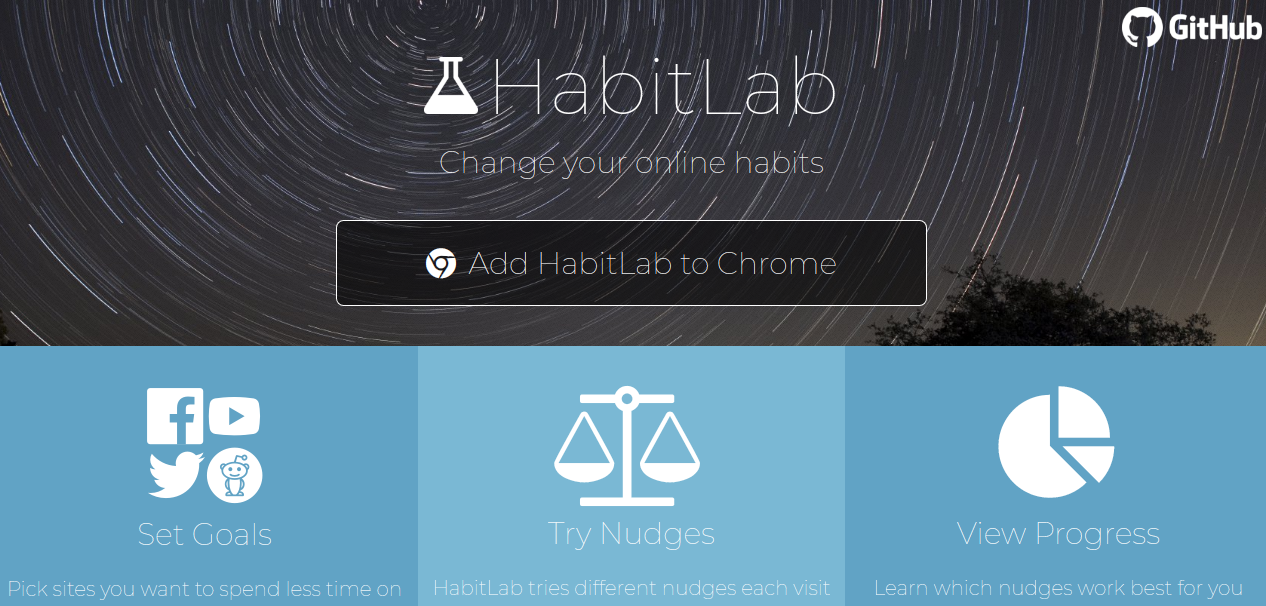
\includegraphics[width=\linewidth]{figures/homepage_cropped}
\caption{HabitLab's homepage describes the browser extension. Users adopt it to try out a large number of different possible interventions, called nudges.}
\label{fig:homepage}
\end{figure}

Users install the extension, and go through an onboarding process where they select sites they wish to reduce their time on (Figure~\ref{fig:onboarding_sites}). There are predefined options---Facebook and YouTube are selected by default, as they were the most commonly used---but users can also add any custom site. Custom sites are suggested via an analysis of the user's browsing history. The system explains to users that they will be shown a variety of interventions (Figure~\ref{fig:onboarding_nudges}), a form of self-experimentation~\cite{Karkar:2017:TFS:3025453.3025480}, to help them reduce time on that site. These interventions are typically targeted to each site, for example a news feed blocker for Facebook or a related video hider for YouTube. However, some interventions such as a stopwatch timer can be added to any custom site. Users can preview the interventions for the sites they select, and enable or disable each intervention if desired. Users can later enable or disable interventions and sites through a settings page.

\begin{figure}
\begin{minipage}[t]{0.49\linewidth}
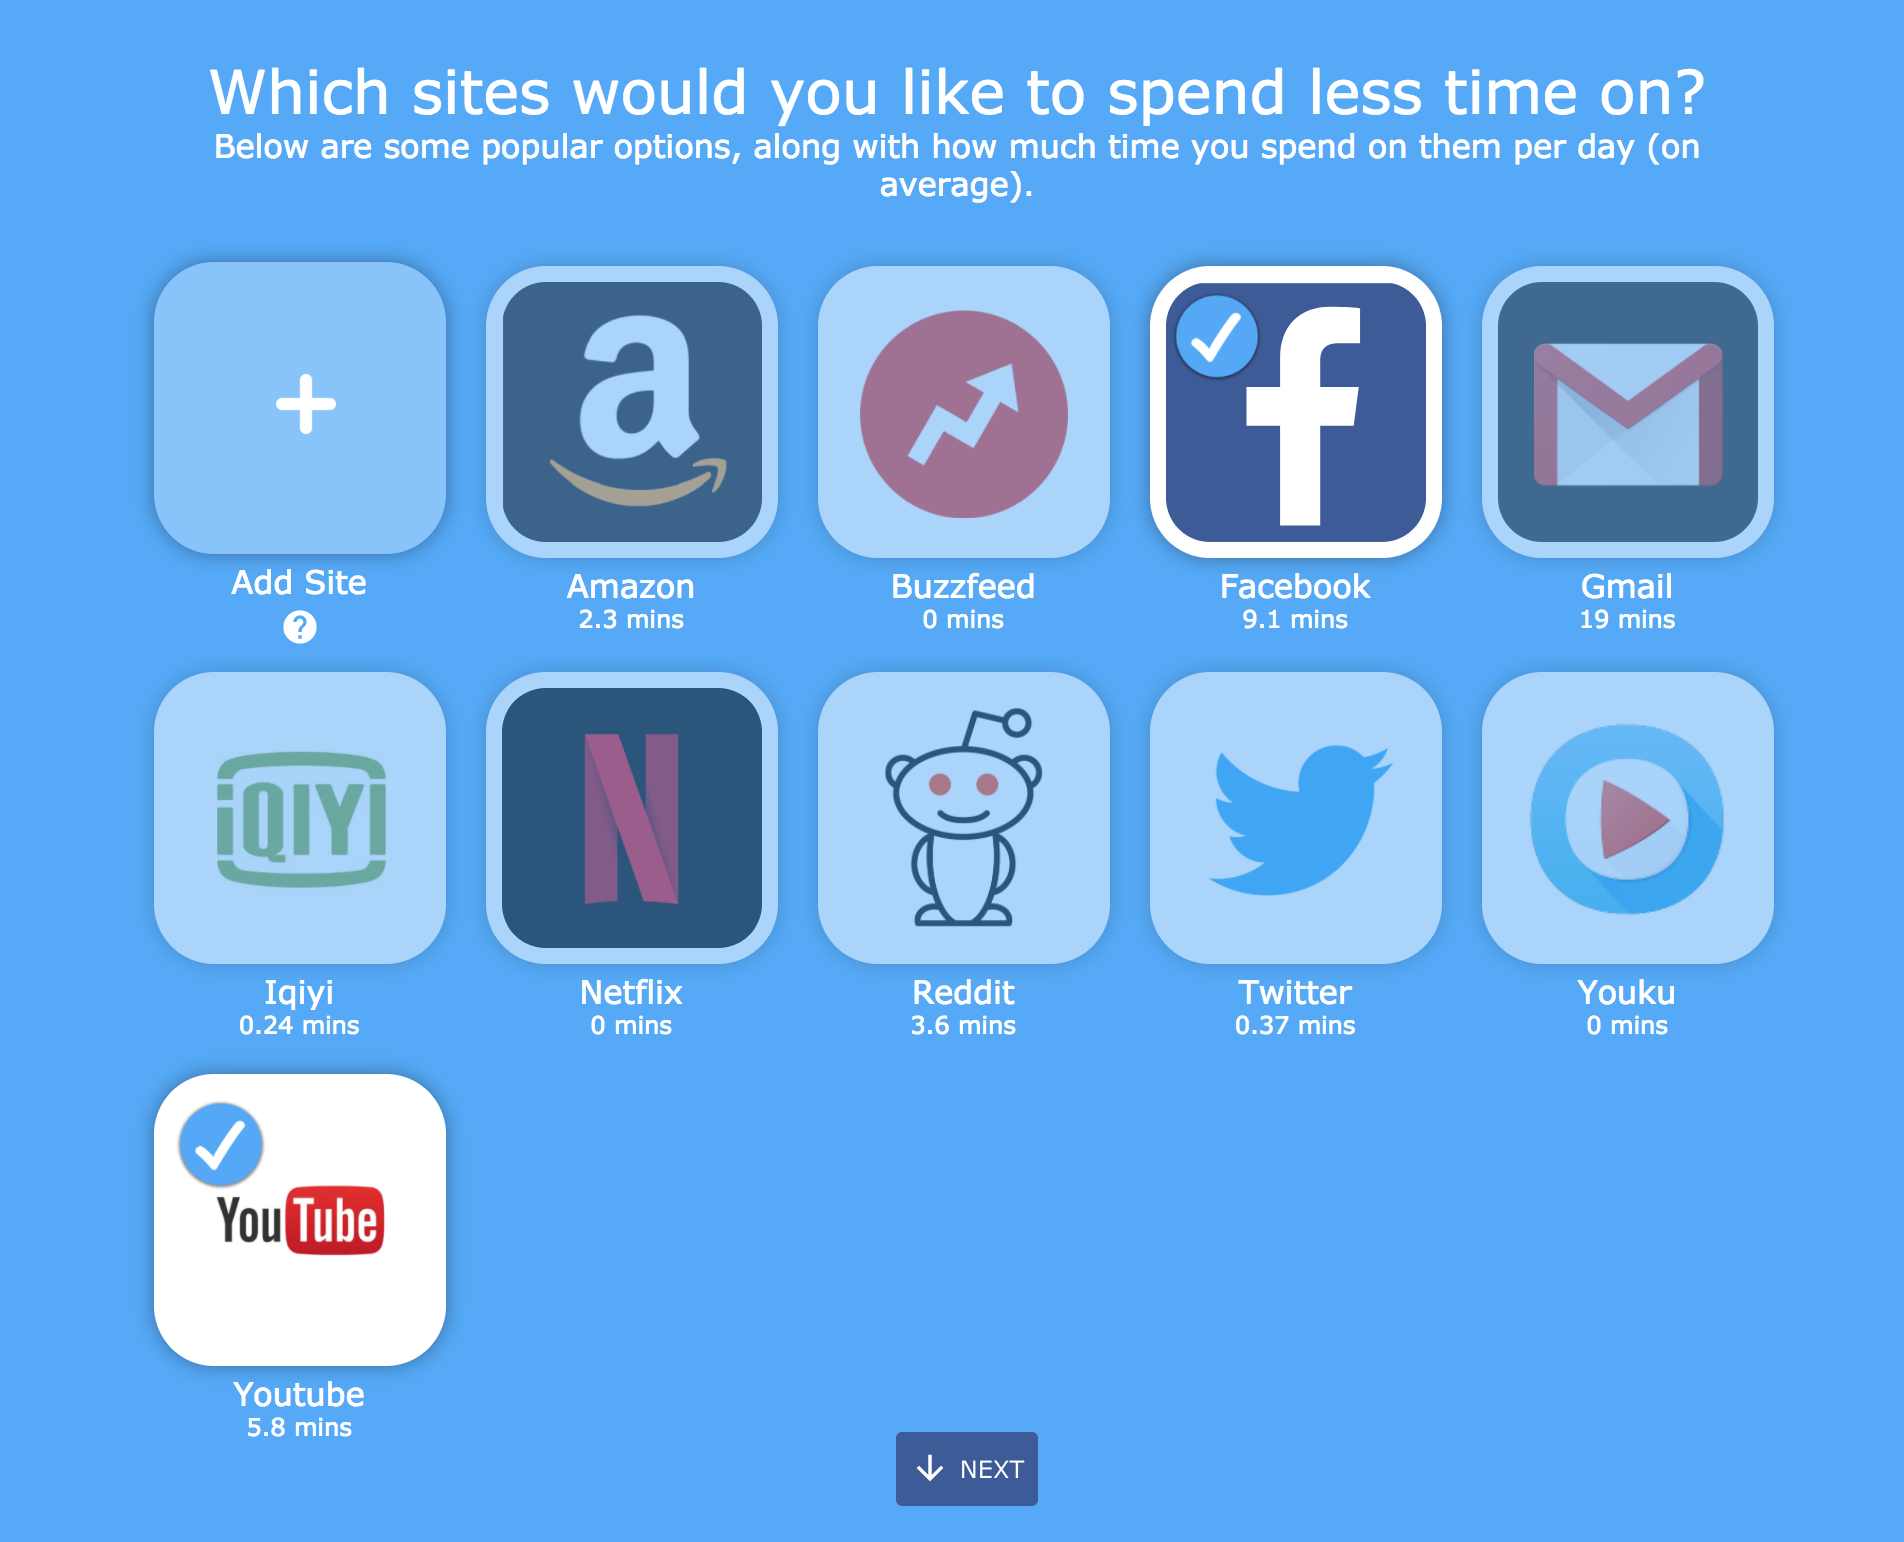
\includegraphics[width=\linewidth]{figures/onboarding_sites}
\caption{During onboarding, users choose which sites they want to spend less time on.}
  \label{fig:onboarding_sites}
\end{minipage}
\hfill
\begin{minipage}[t]{0.49\linewidth}
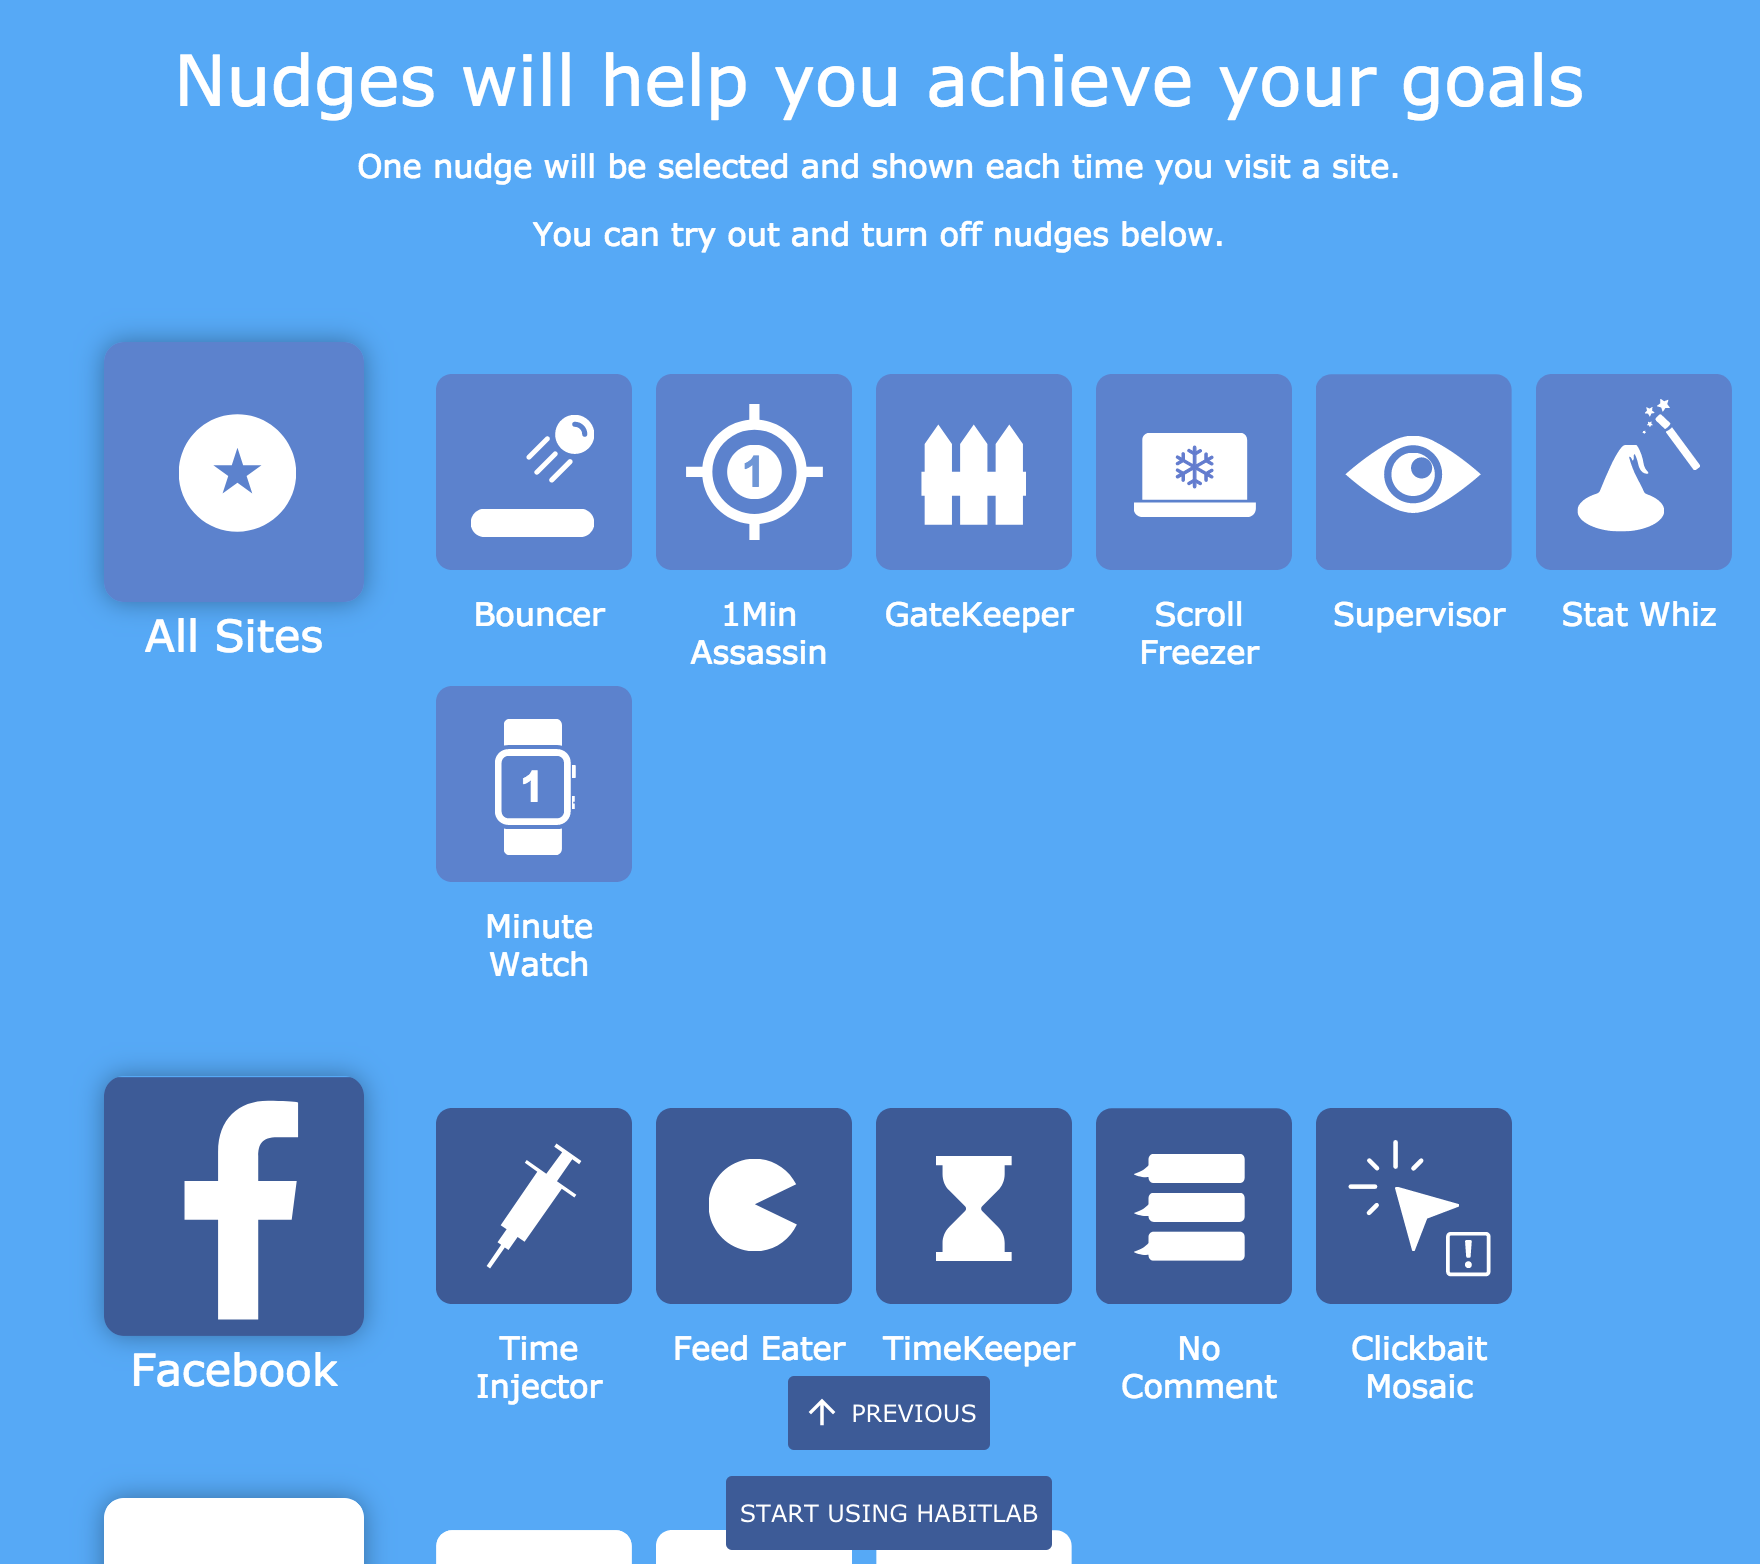
\includegraphics[width=\linewidth]{figures/onboarding_nudges_short}
\caption{Users are presented with the interventions they will see on each site.}
  \label{fig:onboarding_nudges}
\end{minipage}%
\end{figure}

HabitLab emphasizes to users the availability of multiple interventions and that it may show users different interventions each time they load a page. This emphasis is made clear on the HabitLab website, Chrome store listing, and through features in the dashboard such as visualizing the relative effectiveness of different interventions. HabitLab implements a multi-armed bandit algorithm to explore and find the interventions that are most effective for each user, optimizing for minimizing time spent on a site. However, in the experiments in this paper, we disabled this functionality and instead used simple random selection so that we can study the effects of rotation in isolation.

\subsection{Design of HabitLab Interventions}

HabitLab can track time and deploy interventions on all sites, but some interventions are tailored towards specific sites. There are 27 interventions total: seven generic interventions that can be used on all sites, five interventions designed specifically for Facebook, and additional ones designed specifically for YouTube, Reddit, Twitter, Netflix, Gmail, Amazon, iQiyi, and Youku.

Interventions are designed drawing on theories of behavior change---for example, goal setting theory~\cite{locke2002building}, persuasion~\cite{cialdini1987influence,fogg2002persuasive}, and gamification~\cite{deterding2011game}. A sample of the interventions available for Facebook, categorized according to underlying strategies and theories, are shown in Table~\ref{tab:theories}. Screenshots of some Facebook interventions are shown in Figure~\ref{fig:interventions}. %\msb{always use non breaking space \~ between Figure and number, and between sentence and citation block}
% , and health ~\cite{abraham2008taxonomy} \msb{health is not a theory of behavior change}

Not all interventions are enabled by default---this is because some of them have higher attrition rates than others. Non-default interventions can be previewed and enabled by users during onboarding and on the settings page. The interventions enabled by default were the ones we found to have low attrition rates during pilot deployments---we chose this strategy to ensure user retention and growth, which is a prerequisite for gathering data in an in-the-wild experiment setting.

\begin{table}[tb]
\small
\begin{center}
\begin{tabular}{ p{3.3cm} p{3.4cm} p{6.2cm} }
  \textbf{Strategy} & \textbf{Theory} & \textbf{Intervention} \\
  %\hline
  Commitment & Self-consistency theory~\cite{allgeier1979waffle,cialdini1987influence,sherman1980self} & Ask the user to set a goal for the length of time they will stay on the site (generic) \\
  Enforce default limits & Status quo bias ~\cite{samuelson1988status} & Automatically close tab after 60 seconds unless the user clicks a button to ask for more time (generic) \\
%  Enforce default limits & Status quo bias ~\cite{samuelson1988status} & Prevents scrolling unless the user clicks a button to continue scrolling (generic) \\
Reduce social incentives & Social proof~\cite{sherif1935study,cialdini1987influence} & Hide Facebook comments by default (default) \\
  Delaying Rewards & Operant conditioning~\cite{baron1991analyzing} & Make the user wait 10 seconds before visiting Facebook (generic) \\
%  Delaying Rewards & Operant conditioning~\cite{baron1991analyzing} & Shows a page with time spent on Facebook today which they need to click through to get to Facebook (generic) \\
Removing Rewards & Operant conditioning~\cite{baron1991analyzing} & Hide the news feed (default) \\
%  Removing Rewards & Operant conditioning~\cite{baron1991analyzing} & Hide videos and clickbait in the news feed \\
% Gamification & Goal setting theory~\cite{locke2002building}, Flow~\cite{csikszentmihalyi1996flow} & Get points and badges for seeing fewer newsfeed items  \\
  Inform the user & Theory of reasoned action~\cite{ajzen1977attitude} & Show a counter at the top of the page of how long user has been on Facebook today (default, generic) \\
%  Inform the user & Theory of reasoned action~\cite{ajzen1977attitude} & Show a toast notification each minute displaying how long they've been on Facebook today (default, generic) \\
%  Inform the user & Theory of reasoned action~\cite{ajzen1977attitude} & Show a desktop notification each minute displaying how long they've been on Facebook today (generic) \\
% Inform the user & Theory of reasoned action~\cite{ajzen1977attitude} & Inject messages into the news feed showing how long they've been on Facebook today (default) \\
  %Make a plan & Theory of planned behavior \cite{gollwitzer1999implementation} & Ask the user to write out a concrete plan for how they will avoid coming back to the site next time they are tempted to do so \\
  % Rewards/punishment & Operant conditioning~\cite{baron1991analyzing} & Block the site for four hours if the user spends too much time on site in this session \\
  %Stress management & Stress coping~\cite{thoits1995stress} & Reflection on stressors that lead to visiting Facebook \\
  
\end{tabular}
\end{center}
%\vspace{-.7em}
\caption{A subset of the interventions for Facebook, categorized according to persuasion strategy and theory. Interventions that are enabled by default are marked \textit{default}, interventions that are available for all sites are marked \textit{generic}.}
\label{tab:theories}
\end{table}


% todo need to retake these screenshots so they're anonymous
\begin{figure}[tb]
\centering
	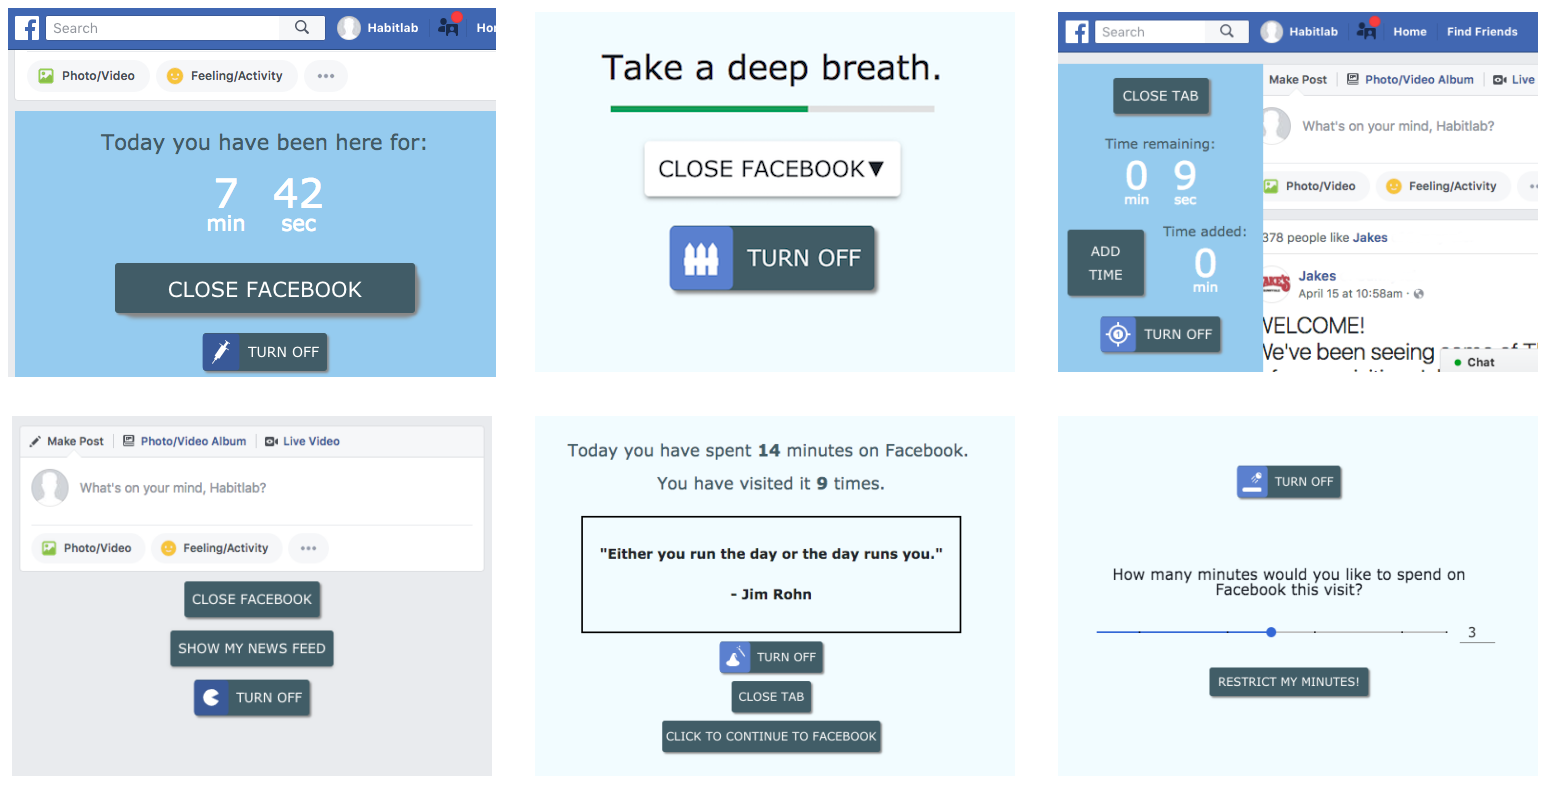
\includegraphics[width=1.0\textwidth]{figures/interventions_new.png}
	\caption{Examples of interventions available for reducing time on Facebook. From left to right, top to bottom: a timer injected into the news feed; a page before opening Facebook requiring that the user wait a few seconds before visiting; a countdown timer that automatically closes the tab after time elapses; an opt-in required to show the news feed; an interstitial page before opening Facebook with a quote; an interstitial page before opening Facebook that requires the user set a time limit for how long they will spend this session.}
\label{fig:interventions}
\end{figure}

\subsection{HabitLab adoption and usage}

As of writing, HabitLab has over \msb{8,000} daily active users from 85 countries (US, India, Germany, France, and the UK are the top 5), and volunteers have translated it into 9 languages (German, French, Spanish, Dutch, Portuguese, Chinese, Czech, Greek, and Turkish).

Users discover the extension through news articles (it has been mentioned in Wired and the New York Times), the Chrome store, or links from an unrelated open-source project by the author. Users are asked to read and provide consent to the research protocol upon installation. They may opt out of data collection if they do not wish to have their data analyzed for research purposes.

% shown in Figure \ref{fig:onboarding_nudges}, some ``generic'' interventions can be used on all sites, and others were developed specifically for a particular site such as Facebook or Youtube.

%\begin{figure}
%  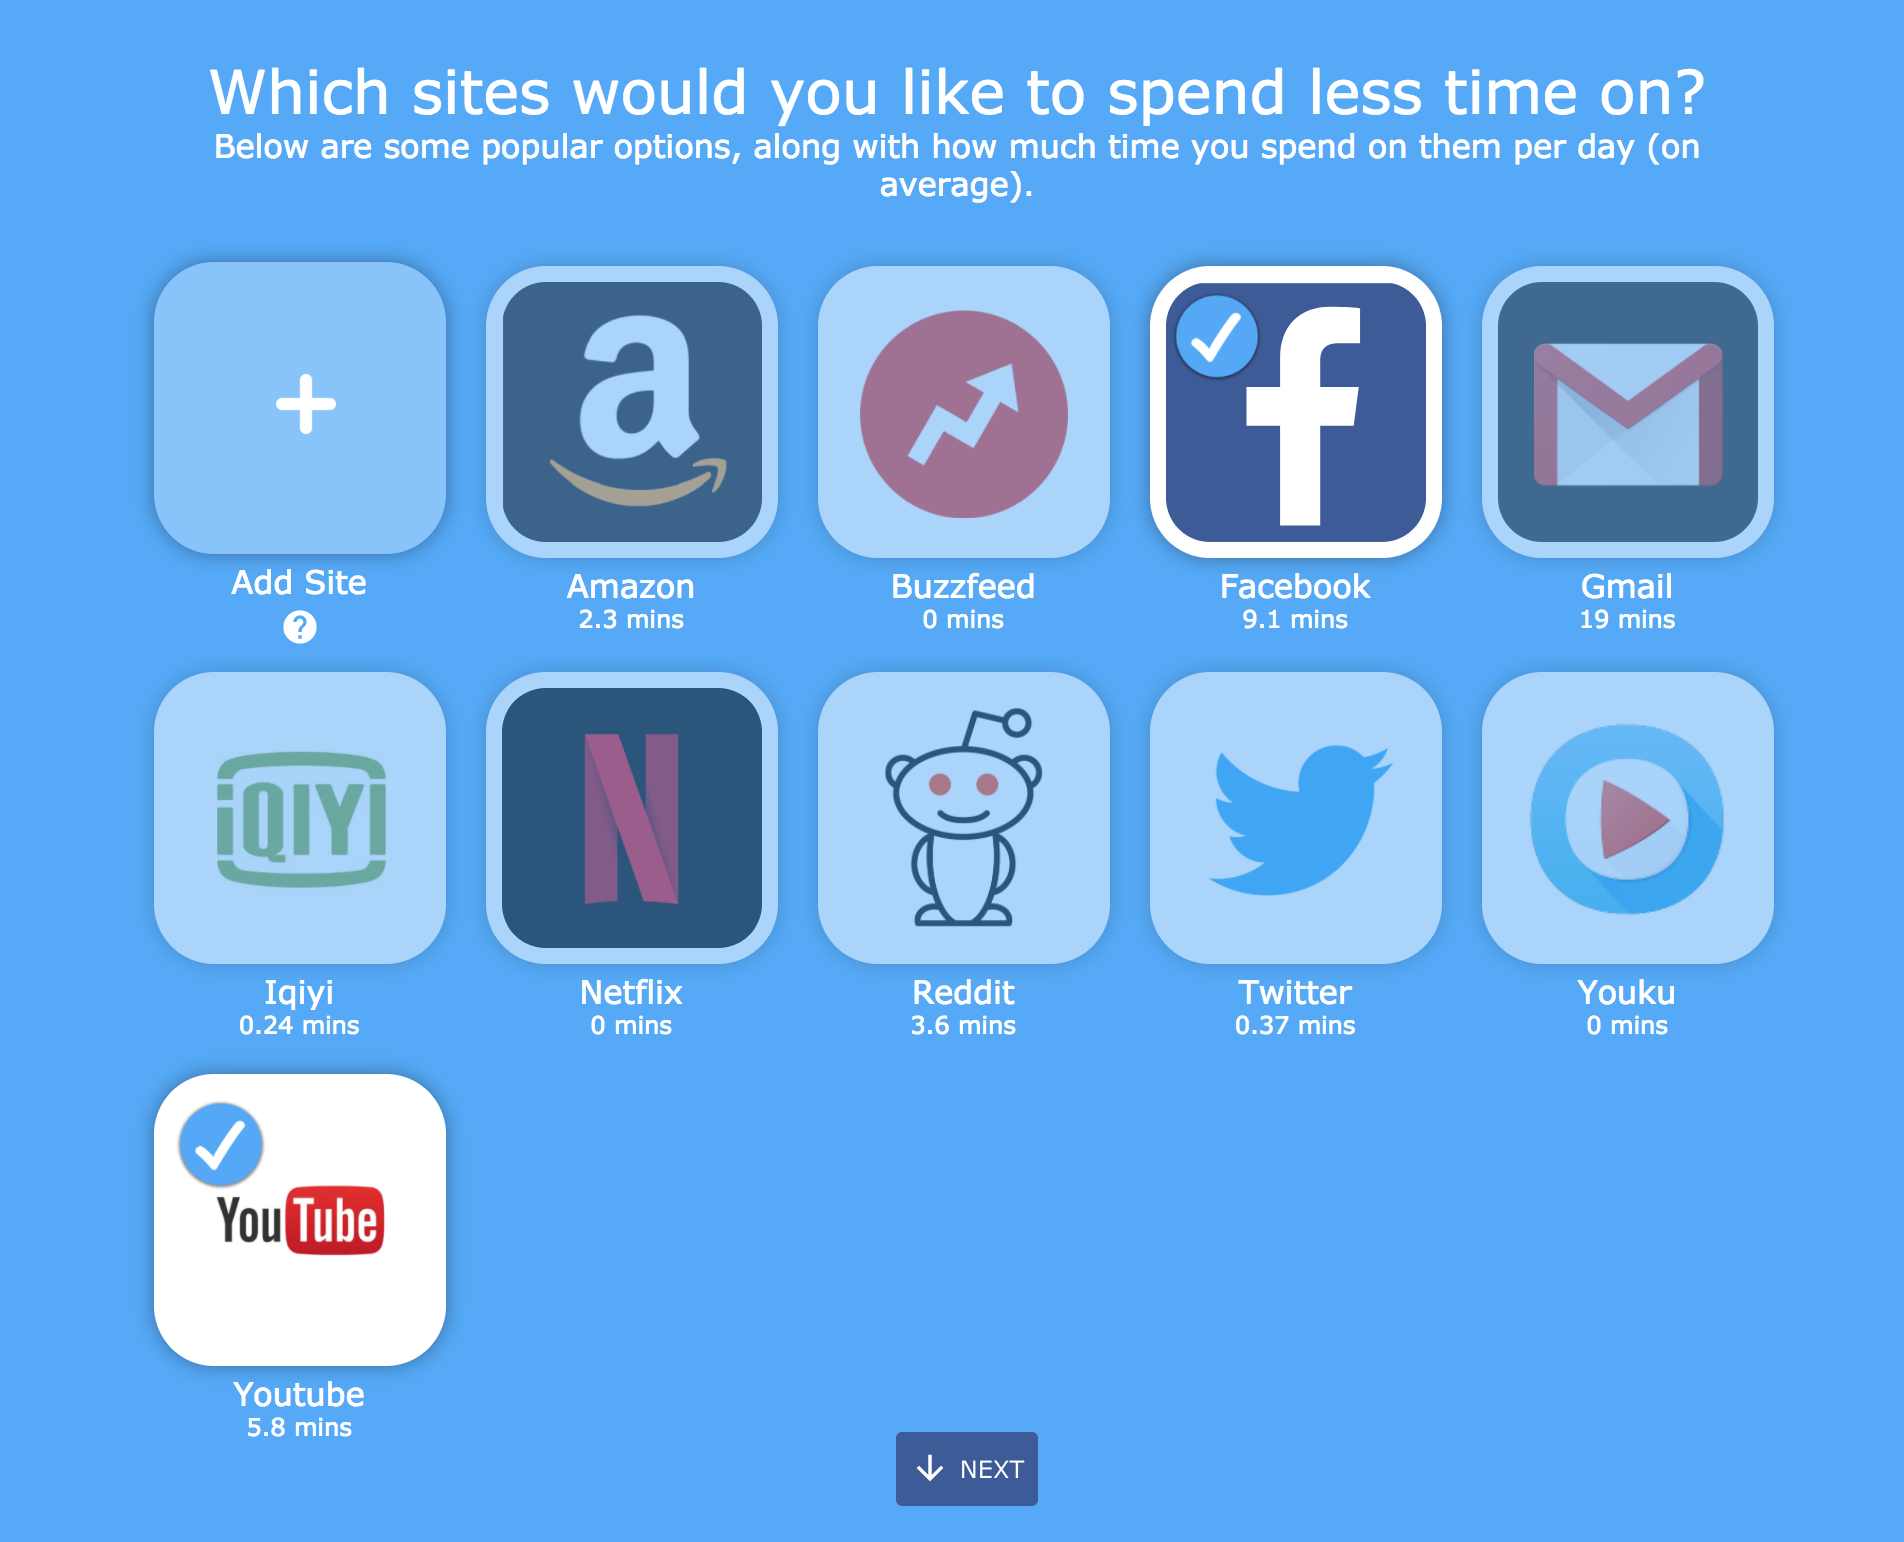
\includegraphics[width=\textwidth]{figures/onboarding_sites}
%  \caption{During onboarding, users first select sites to spend less time on.}
%  \label{fig:onboarding_sites}
%\end{figure}

%\begin{figure}
%  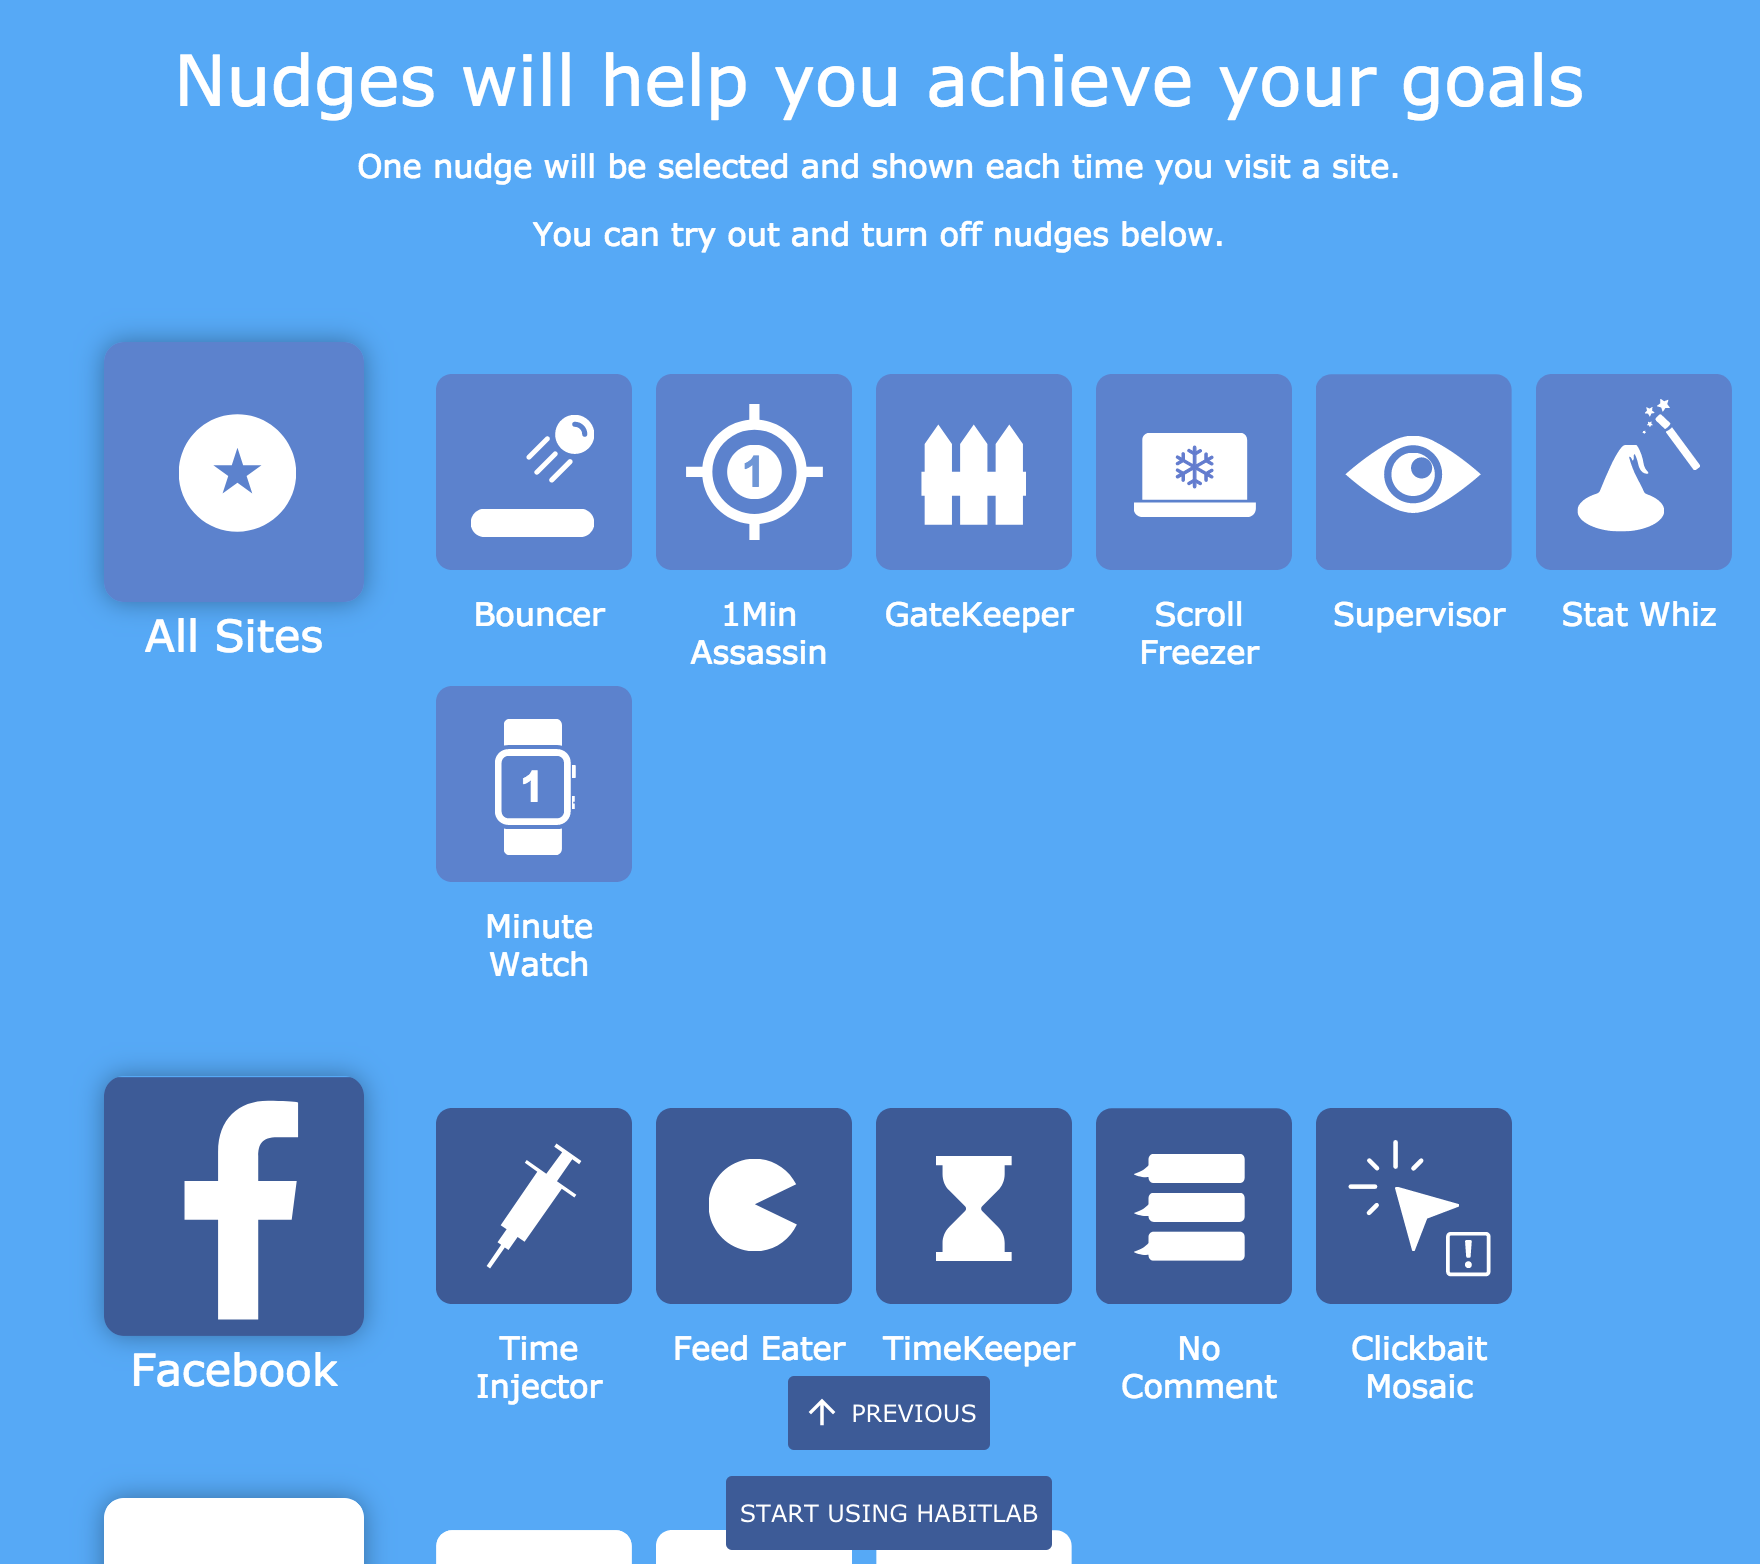
\includegraphics[width=\textwidth]{figures/onboarding_nudges_short}
%  \caption{Users are then presented with the nudges (interventions) they will see on each site.}
%  \label{fig:onboarding_nudges}
%\end{figure}


\section{Study 1: Field Study on the Effect of Rotating Interventions}

Our first study is a within-subjects design run on the HabitLab platform that aims to understand the effects of rotating interventions on effectiveness and attrition.

\subsection{Participants}

% todo confirm it was actually 3 weeks

% Participants in our first study consisted of new HabitLab users installing the system over a period of three weeks in March and April 2018. 217 users installed HabitLab over the course of our experiment and consented to our research protocol. We discarded participants who were not new users of HabitLab, since some users were reinstalls or new devices for existing users. We also discarded participants who did not the complete the onboarding process, or who uninstalled the system before they saw their first intervention.

Participants in our first study consisted of new HabitLab users installing the system over a period of three weeks in March and April 2018. 692 users installed HabitLab over the course of our experiment and consented to our research protocol. We discarded participants who were not new users of HabitLab, since some users were reinstalls or new devices for existing users. We also discarded participants who did not the complete the onboarding process, or who uninstalled the system before they saw their first intervention. This left us with 217 participants. %\msb{didn't we also filter out people who manipulated the default settings?} \gezacomment{no that was the other study, this one bypassed that issue because the static selection algorithm continued choosing the same intervention even if they had multiple enabled} % For this study, we focus only on users who enabled interventions for Facebook. This final subset consists of 55 participants.

% Participants in our first study consisted of new HabitLab users installing the system over a period of three weeks in March and April 2018. 217 users installed HabitLab over the course of our experiment and consented to our research protocol. We discarded participants who were not new users of HabitLab, since some users were reinstalls or new devices for existing users. We also discarded participants who did not the complete the onboarding process, or who uninstalled the system before they saw their first intervention. For this study, we focus only on users who enabled interventions for Facebook. This final subset consists of 55 participants. \msb{didn't we also filter out people who manipulated the default settings?} \gezacomment{no that's study 0 which we're leaving out of this paper} % \msb{they are users in the context of a system; participants in the context of a study} 

% are reviewers not going to like that our userbase is 89% male?

%\msb{general rule: do not use parentheticals in writing. either 1) the statement is important enough to be a full member of the sentence, in which case you should promote it out of the parens; or 2) it's not important enough to be a full member, in which case you should cut it. I'm editing out a ton of parentheticals, 1-2 per paragraph at this point}

We do not administer a demographic survey at install time, because long onboarding processes had previously led to high abandonment. Many users find HabitLab through routes other than the web site, but Google Analytics on the web site can provide some window into rough trends. Google Analytics estimates that 89\% of visitors to the HabitLab website during the experiment period were male, indicating a male skew. The most common age group was 25--34 (41\%), followed by 18--24 (29\%), 35-44 (22\%), and 45--54 (7\%). According to users' IP addresses, the most highly represented countries were the US (23\%), India (12\%), Germany (9\%), France (5\%), and the UK (4\%).

%\msb{Tweaked and moved up to the Participants section:}

Participants agreed to our informed consent protocol during onboarding. This consent protocol indicated that HabitLab would be selecting and rotating between different interventions, but did not mention any specific algorithm or rotation schedule.

\subsection{Method}
%\msb{The entire title and intro use ``static`` and ``rotation'', we need to be consistent. I'm changing to rotation but if you want ``random'' and ``same'' let's talk and align.}

Participants used HabitLab in the course of their usual web activity. As they browsed, HabitLab would introduce interventions when appropriate. All interventions were available to all conditions, but the pace at which old interventions were replaced by new ones depended on condition. Users would react to the intervention, or not, as they browsed. %HabitLab tracked two measures: how long they spent on the site each day, and if they exhibited attrition. 

HabitLab operated on all web sites that the user had selected upon installation. However, because users spend differing amounts of time on different domains, and there was a long tail of domains which were set as goal sites by only a few users, we restricted analysis to domains where we had a substantial dataset, specifically: Facebook, Youtube, Reddit, Twitter, VK, and Amazon. % (a Russian social network)

% generated from figures/experiment1_design_figure.pptx

\begin{figure}[tb]
\centering
	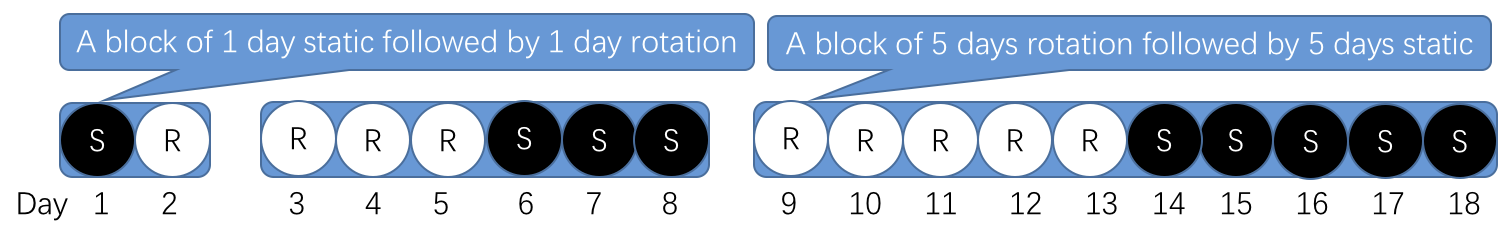
\includegraphics[width=1.0\textwidth]{figures/experiment1_design_figure_v2.png}
	\caption{Example order in which a user might see conditions. Each circle represents a day -- on black days the user is in the ``static'' condition, white is the ``rotation'' condition. The order of blocks is randomized; here, this participant is seeing blocks in order 1, then 3, then 5, then 7 (omitted in the figure).}
\label{fig:experiment1_design_figure}
\end{figure}

The experimental unit was a participant assigned to a condition for a block of days. Block lengths were randomized between 1 day, 3 days, 5 days, and 7 days, in order to give us insight into the effects of rotation strategy over different time horizons. When participants were randomized to a block, for example a five-day block, they experienced HabitLab in one condition for five days, then in the other condition for five days, for a total of ten days (Figure~\ref{fig:experiment1_design_figure}). Condition order was randomized within each block. At the conclusion of a block, the user was then moved into another block length and the trial repeated. The sequence of block lengths was randomized for each participant. If they kept the system installed, participants would experience all blocks after 32 days.

\subsection{Conditions}
We developed a within-subjects repeated measures design, where users alternated between blocks of time during which they were shown either a static intervention or rotated interventions. A within-subjects design such as this allows us to better control for the large variability across users in how much time they spend on a site.

The static condition captures a typical behavior change design with one strategy. At install time, for each site, the participant is randomly assigned a single intervention among the ones that are enabled for the site. Whenever they visit that site on a day in the static condition, the participant will always see that intervention, i.e. the static intervention is the same across all blocks.

The rotation condition captures a strategy of keeping the interventions changing so that users do not begin ignoring them. Each time a participant in the rotation condition visits a target site (e.g., Facebook), HabitLab picks a random intervention from the enabled set to display.

So, in a five day block, a user might spend five days in the static condition seeing the same intervention each time, then five days in the rotation condition seeing randomly selected interventions each time. They are then moved into another block and the method repeats.

\subsection{Measures}

We measured the \textit{effectiveness} of the system as the number of seconds spent on the target site each day. Time, of course, does not perfectly correspond to attention or engagement behavior, as users can get distracted and not actually attend to a web page. However, prior work has generally found it to be an effective estimate (e.g.,~\cite{whittaker2016don}). %We refine our time tracker to measure time the same way that the Chrome browser does: active time is counted as the tab focused, window focused, and mouse or keyboard movement within the past minute. 
To determine whether the user is actively using a target site, we use Chrome's internal definition of active --- the browser window and tab is focused, the computer screen is on, and there has been mouse or keyboard activity on the tab within the past minute. 
%We aggregate our measurements at two levels: sessions and days. Time on site per session is measured as the total time the user was actively using a site in a browser tab, from when they visited the site until they closed the tab.
%If the user switches tabs to a different site, the time spent on the other site is not counted towards the current session time. 
Time on site per day is measured as the aggregated time across sessions from midnight to midnight in the participant's local timezone.
There was %one session data point per user per session per web site, and 
one data point per user per day per targeted web site.
Because time data is not normally distributed, we adopt a common practice of log-transforming the time data prior to analysis.


%We measured \textit{attrition} as the number of days the participant kept the extension enabled. We also noted if the extension was still enabled at the conclusion of our study. The browser does not reliably send a notification to our server if a user disables or uninstalls the extension, so we coded instances of attrition when the server stopped receiving data from the user for over two days, with no later resumption.

We measured \textit{attrition} as the number of days the participant kept the extension enabled. We also noted if the extension was still enabled at the conclusion of our study. The browser does not send a notification to our server if a user disables the extension, so we coded instances of attrition when the server stopped receiving data from the user for over two days, with no later resumption.

As with many online field experiments, effective data cleaning is essential to accurate analysis. We excluded users who had HabitLab installed on multiple devices, to focus on site usage on a single device. %For measurements of time on site per day, w
We discarded days on which the target site was never visited, as in neither condition would the intervention have been shown. %For measurements of time on site per day, w
We also discarded the first day because participants installed the extension midway through the day, resulting in an underestimate at the day level; we likewise discarded any days on which the user uninstalled or disabled the extension, as this would again cause the measured time to be an underestimate of the actual time spent on site that day.

\subsection{Method of Analysis}

For analyzing effectiveness at both the day and session level, we used a linear mixed model (LMM). We used an LMM because we have multiple samples from each user, but the number of samples from each user and in each condition is variable (because attrition may occur before they completed all conditions, or they may not visit a site on a particular day), which violates the assumptions of the repeated-measures ANOVA. 

%Upon installation, users chose which sites they want HabitLab to track. Because users spend differing amounts of time on different domains, and there was a long tail of domains which were set as goal sites by only a few users, we restricted analysis to the top 5 domains that our participants marked as wanting to spend less time on: Facebook, Youtube, Reddit, Twitter, and VK (a Russian social network).

To test whether interventions decrease in effectiveness over time (H\ref*{hyp:decreaseovertime}), we focused on just data points from the static condition. The model included a term for the number of days that particular intervention had previously been seen,\footnote{Repeating the analysis using the number of times the intervention had been seen yields the same conclusions.} a random effect for the participant, and a random effect for domain. To test linear mixed models for significance, we used a likelihood ratio test to compare a reduced model without the number of days predictor to the full model. A significant test indicates that the number of days has statistically significant explanatory power, analogous to a significant beta coefficient in a traditional regression.

To test whether static or rotated interventions increase effectiveness (H\ref*{hyp:rotation}), we used data from both the static and rotation conditions. This second LMM, predicting log time spent on the site each day, included a random effect for participant, a random effect for domain, a fixed effect for block length, and a fixed effect for condition. A likelihood ratio test compared to a reduced model without the condition variable. 

To analyze whether static or rotated interventions increase attrition (H\ref*{hyp:attrition}), we %used a pair of analyses. First, a generalized linear mixed model (GLMM) predicted whether attrition would occur after each session. Because attrition is a binary variable in this context, a GLMM with binomial (logistic) link function is more appropriate than an LMM. The model included the same predictors as above, and is also tested against a reduced model using a likelihood ratio test. 
%To analyze attrition effects over longer (block-length) periods, we 
used a Cox proportional hazards regression. Cox proportional hazards models predict the relative ``hazard'' (i.e. risk) of attrition given each predictor. This is used in the health sciences for estimating expected lifetimes when we may have differing durations of observations for each participant, and may have observed deaths (which correspond to attrition) for some participants but not others. Each data point consists of a point of observation, and whether the participant had experienced attrition at that point or was still active. To avoid crossing conditions in this analysis, we focus the Cox analysis on just each user's first assigned block and condition, for example a seven-day rotation block or three-day static block. Each observation consists of the length of block, and whether the user had experienced attrition by the end of the first condition for their first block. The Cox model used a single predictor: condition. The output of a Cox proportional hazards model is similar to a regression, with a significance value and estimate attached to the predictor.

% \section{Study 1 Methodology}

% We used a within-subjects repeated measures design, where users alternated between blocks of time during which they were shown either the same intervention for N days (where N is selected randomly from either 1,3,5, or 7), or random interventions each visit for N days, followed by the opposite condition (random counterbalanced). We chose a within-subjects design because there is extreme variability in how much time users spend on each site, making this unsuitable for a between-subjects design. Users were assigned. Due to natural user attrition over time and the fact that 

% 196 users installed HabitLab over the course of our experiment, but we discarded users who were not new users of HabitLab (some users were reinstalls or new devices for existing users), and we discarded users who stopped using the system within the first day (the majority of attritions occur within the first 5 minutes, due to users installing extensions simply to explore and compare them). Our analysis will focus only on users who used our Facebook interventions, which leaves us with 55 users.

% Users were divided into . Exact demographics are unknown but Google Analytics estimates that X\% of visitors to the HabitLab website are (fill in). Users are globally distributed from (fill in).


\subsection{Results}

In this study, participants had an average of 3.0 target sites enabled. They visited at least one target site 67\% of days on average. On each of those days, participants experienced interventions an average of 3.6 times. \rev{We did not receive any feedback indicating that participants were aware of patterns in how HabitLab was rotating interventions.}

% summary_stats_study1.py
% num domains per user: mean 3.0 stddev 1.8
% fraction time seen: mean 0.96 stddev 0.6
% num sessions per day: mean 3.6 stddev 5.3

% \msb{Report a general statical overview here first. For example, what is the average number of sessions per participants per site per day?}

% Our analysis focuses on two levels of measurement: sessions and days.

% Time on Facebook per day is measured as the total time the user was actively using Facebook in the browser (with "active" being the same definition that the Chrome browser uses - tab focused, window focused, and mouse or keyboard movement within the past minute). The day starts from midnight in the local timezone. Because we excluded users who had HabitLab installed on multiple devices, we are considering only Facebook usage on a single device.

% Time on Facebook per visit is measured as the total time the user was actively using Facebook in a browser tab, from when they visited Facebook until they closed the tab. If the user switches tabs to a different site, the time spent on the other site is not counted towards the current Facebook session time.

% We discarded days on which Facebook was not visited at all. For measurements of time on Facebook per day, we discarded the first day, as the user may install midway through the day so the measured time that day would be an underestimate. For measurements of time on Facebook per day, we discarded any days on which a user attritioned (which can result from uninstalling or disabling the extension), as this would again cause the measured time to be an underestimate of the actual time spent on site that day.

% We analyzed our data using a linear mixed model. We used this because we have multiple samples from each user, but the number of samples from each user and in each condition is variable (because users may attrition before they completed all conditions, they may not visit a site on a particular day), which violates the assumptions of the repeated-measures ANOVA.

% how to report data from a linear mixed model: https://arxiv.org/ftp/arxiv/papers/1308/1308.5499.pdf

% You	would	report	this result	the	following	way:
% “…	 politeness	 affected	 pitch	 (χ2(1)=11.62,	 p=0.00065),	 lowering	 it	 by	
% about	19.7 Hz	± 5.6	(standard	errors)	…”
\subsubsection{Effectiveness of interventions over time}
First we examine whether interventions decrease in effectiveness over time within the static condition. If so, rotation may be a viable strategy.



%Interventions decrease in effectiveness over time (as evidenced by longer visit times on site), both if we measure it according to the number of days on which the intervention has been previously seen at least once, or if we measure it according to number of total times that the intervention has been seen.

The likelihood ratio test confirms that the number of days the user had seen the static intervention affected the log of time spent on a domain per day ($\chi^{2}(1) = 4.69, p < 0.05$), supporting H\ref*{hyp:decreaseovertime}. Each day the intervention has been previously seen increased the log time spent by 0.225 (Table~\ref{tab:effectiveness_sessions_alldomain_vs_num_days_same}). By exponentiating the log estimates, this translates into an increase of 25\% on top of a baseline 117 seconds per day for each additional day the user were exposed to the static intervention. %during the study. %Note that since the dependent variable is log time rather than raw time, this 15\% estimated increase is multiplicative for each additional day. 
%An alternative method of analysis, where we measure the raw number of times the intervention has been seen instead of the number of days it has been seen, yields the same results. \msb{still correct?} %\msb{does an equivalent analysis at the day level yield the same results? otherwise why did we make such a big deal of having both session and day data? If we're going to report both, we need to report both for all studies. Otherwise we need to cut and use just one.} %Restricting analysis to just Facebook also yields the same results.

%\msb{This paragraph doesn't make sense to me: the method section said that this dataset considered only static days:} Note that we observed a significant decline in effectiveness if we analyze days where users were assigned to the static condition, but the decline is not significant on days when the user is in the rotation condition. This suggests that if interventions decline in effectiveness in the rotation condition, it is occurring at a rate too slow to be observed with our study.

% Table created by stargazer v.5.2 by Marek Hlavac, Harvard University. E-mail: hlavac at fas.harvard.edu
% Date and time: Wed, Apr 18, 2018 - 18:19:53
% Table created by stargazer v.5.2 by Marek Hlavac, Harvard University. E-mail: hlavac at fas.harvard.edu
% Date and time: Wed, Apr 18, 2018 - 18:50:23
\begin{table}[tb] \centering 
  \caption{Within the static condition, interventions decline in effectiveness. Longer visit lengths increase with the number of days seeing the same static intervention.} 
  \label{tab:effectiveness_sessions_alldomain_vs_num_days_same} 
\begin{tabular}{@{\extracolsep{5pt}}lc} 
\\[-1.8ex]\hline 
\hline \\[-1.8ex] 
 & \multicolumn{1}{c}{\textit{Dependent variable:}} \\ 
\cline{2-2} 
\\[-1.8ex] & Log time spent per day \\ 
\hline \\[-1.8ex] 
 Number of days the user had seen the static intervention & 0.225$^{*}$ \\ 
  & (0.097) \\ 
  (Intercept) & 4.759$^{***}$ \\ 
  & (0.392) \\ 
 \hline \\[-1.8ex] 
Observations & 124 \\ 
\hline 
\hline \\[-1.8ex] 
\textit{Note:}  & \multicolumn{1}{r}{$^{*}$p$<$0.05; $^{**}$p$<$0.01; $^{***}$p$<$0.001} \\ 
\end{tabular}
\vspace{1em}
\end{table} 


%First we ran a Shapiro test of normality to find that the response variable (log of session times) is indeed normally distributed: W = 0.97751, p-value = 3.724e-06 TODO it looks like it's not actually, probably need to switch to a GLMM

%shapiro.test(data_facebook$log_time_spent)



%We used a chi-squared test to compare the following two linear mixed effects models for predicting the log of time spent on Facebook per session:

%Full model: number of days the intervention has been previously seen [fixed effect], intervention [fixed effect], user [random effect]

%Reduced model: intervention [fixed effect], user [random effect]

% results <- lmer(log_time_spent ~ num_days_intervention_seen_at_least_once + as.factor(intervention) + (1|install_id), data = data_facebook)
% resultsnull <- lmer(log_time_spent ~ as.factor(intervention) + (1|install_id), data = data_facebook)

%The number of days the intervention has been previously seen affected the log of time spent on Facebook per visit ($\chi^{2}(1)$ = 4.4276, p = 0.03536), with each day the intervention has been previously seen increasing it by an estimate of 0.06738 (standard error = 0.03171, t-value = 2.125) from an intercept of 3.82230 (standard error = 0.29295, t-value = 13.047).

%            Df    AIC    BIC  logLik deviance  Chisq Chi Df Pr(>Chisq)  
%resultsnull  7 1622.2 1650.6 -804.10   1608.2                           
%results      8 1619.8 1652.2 -801.88   1603.8 4.4276      1    0.03536 *

%                                                    Estimate Std. Error t value
%(Intercept)                                          3.82230    0.29295  13.047
%num_days_intervention_seen_at_least_once             0.06738    0.03171   2.125

%This translates into an increase of 7\%, or 3 seconds per visit each additional day that an intervention has been previously seen (we calculated these using $firstday=e^{intercept}=e^{3.82230}=46$ and $nextday=e^{intercept+estimate}=e^{3.82230+0.06738}=49$ -- note that since the linear mixed effects model is fitting its estimate to the log of time spent, this estimated increase is multiplicative when translated back to raw time).

%QUESTION: do we want to include the below at all? \msb{no, I compressed it}

%We used a chi-squared test to compare the following two linear mixed models for predicting the log of time spent on Facebook per session:

%Full model: number of times the intervention has been previously seen [fixed effect], intervention [fixed effect], is it the first time the user is visiting Facebook today [fixed effect], user [random effect]

%Reduced model: intervention [fixed effect], is it the first time the user is visiting Facebook today [fixed effect], user [random effect]

%results <- lmer(log_time_spent ~ impression_idx + is_first_visit_of_day + as.factor(intervention) + (1|install_id), data = data_facebook)
%resultsnull <- lmer(log_time_spent ~ is_first_visit_of_day + as.factor(intervention) + (1|install_id), data = data_facebook)

%The number of times the intervention has been previously seen affected the log of time spent on Facebook per visit ($\chi^{2}(1)$ = 4.7703, p = 0.02896), with each time the intervention has been seen increasing it by an estimate of 0.008059 (standard error = 0.003675, t-value = 2.193) from an intercept of 3.283771 (standard error = 0.340267, t-value = 9.651).

%This translates into an increase of TODO 7\%, or 3 seconds per visit each additional time that an intervention has been previously seen (we calculated these using $firsttime=e^{intercept}=e^{3.283771}=46$ and $nexttime=e^{intercept+estimate}=e^{3.82230+0.06738}=49$ -- note that since the linear mixed model is fitting its estimate to the log of time spent, this estimated increase is multiplicative when translated back to raw time).

%                                                     Estimate Std. Error t value
%(Intercept)                                          3.283771   0.340267   9.651
%impression_idx                                       0.008059   0.003675   2.193
%is_first_visit_of_day                                0.676552   0.214924   3.148

%            Df    AIC    BIC  logLik deviance  Chisq Chi Df Pr(>Chisq)  
%resultsnull  8 1617.4 1649.8 -800.72   1601.4                           
%results      9 1614.7 1651.1 -798.33   1596.7 4.7703      1    0.02896 *

\subsubsection{Effectiveness of rotation and static intervention strategies}

%The likelihood ratio test found a significance difference between the full and reduced models predicting effectiveness ($\chi^{2}(1) = 6.31, p < 0.05$), indicating that condition significantly impacted effectiveness. Relative to the rotation condition, static interventions increased the log time spent on Facebook per day by 0.7549 (Table~\msb{REGRESSION TABLE TODO}). Exponentiating for descriptive purposes, this translates into a shift from an estimated 219 seconds per day in the random condition to 466 seconds per day in the rotation condition, an increase of 247 seconds per day.

Next, we compare whether the daily time spent on domains differs between days when participants were in the rotation and static conditions.

The likelihood ratio test found a significance difference between the full and reduced models predicting effectiveness ($\chi^{2}(1) = 4.88, p < 0.01$), indicating that condition significantly impacted effectiveness. Relative to the static condition, rotating interventions decreased the log time spent on domains per day by 0.417 (Table~\ref{tab:effectiveness_same_vs_random}), supporting H\ref*{hyp:rotation}. Exponentiating the coefficients for descriptive purposes, this translates into a shift from an estimated 146 seconds per day in the static condition to 96 seconds per day in the rotation condition, a decrease of 50 seconds (34\%) per day.

%An alternative analysis that yields the same result by looking at time spent per session rather than day is shown in the appendix.

%An alternative analysis that yields the same result is to restrict analysis to Facebook on days where more than 1 intervention was seen.

%The likelihood ratio test found a significance difference between the full and reduced models predicting effectiveness ($\chi^{2}(1) = 9.74, p < 0.005$), indicating that condition significantly impacted effectiveness. Relative to the rotation condition, static interventions increased the log time spent on Facebook per day by 0.7549 (Table~\ref{tab:effectiveness_facebook_same_vs_random}). Exponentiating for descriptive purposes, this translates into a shift from an estimated 212 seconds per day in the random condition to 486 seconds per day in the rotation condition, an increase of 274 seconds per day.

% Table created by stargazer v.5.2 by Marek Hlavac, Harvard University. E-mail: hlavac at fas.harvard.edu
% Date and time: Wed, Apr 18, 2018 - 18:27:32
\begin{table}[tb] \centering 
  \caption{Daily time spent on sites in the static and rotation conditions. Users spend less time per day on sites in the rotation condition.} 
  \label{tab:effectiveness_same_vs_random} 
\begin{tabular}{@{\extracolsep{5pt}}lc} 
\\[-1.8ex]\hline 
\hline \\[-1.8ex] 
 & \multicolumn{1}{c}{\textit{Dependent variable:}} \\ 
\cline{2-2} 
\\[-1.8ex] & Log time spent per day \\ 
\hline \\[-1.8ex] 
 Rotation (baseline: static) & $-$0.417$^{*}$ \\ 
  & (0.190) \\ 
  Block length & 0.018 \\ 
  & (0.048) \\ 
  (Intercept) & 4.981$^{***}$ \\ 
  & (0.346) \\ 
 \hline \\[-1.8ex] 
Observations & 370 \\ 
\hline 
\hline \\[-1.8ex] 
\textit{Note:}  & \multicolumn{1}{r}{$^{*}$p$<$0.05; $^{**}$p$<$0.01; $^{***}$p$<$0.001} \\ 
\end{tabular} 
\vspace{1em}
\end{table} 


%In the days where users were shown the high-novelty condition (where users are shown random interventions each visit), overall time spent on Facebook is less than in the low-novelty days (where users are shown the same intervention).

%First we ran a Shapiro test of normality to find that the response variable (log of daily time spent on Facebook) is indeed normally distributed: W = 0.97878, p-value = 0.118

%shapiro.test(datadays_facebook$log_time_spent)

%We used a chi-squared test to compare the following two linear mixed models for predicting the log of time spent on Facebook per day:

%Full model: condition ("same" or "random") [fixed effect], user [random effect]

%Reduced model: user [random effect]

% results <- lmer(log_time_spent ~ as.factor(condition) + (1|install_id), data = datadays_facebook_withoutattritionday)
% resultsnull <- lmer(log_time_spent ~ (1|install_id), data = datadays_facebook_withoutattritionday)

%The condition affected the log of time spent on Facebook per day ($\chi^{2}(1)$ = 6.3094, p = 0.01201), with condition=same increasing it by an estimate of 0.7549 (standard error 0.2982, t-value = 2.532) from an intercept of 5.3903.

%This translates into an increase of 247 seconds per day (from 219 seconds with random, to 466 in the same condition -- we calculated these using $random=e^{intercept}=e^{5.3903}=219$ and $same=e^{intercept+estimate}=e^{5.3903+0.7549}=466)$.

% you might ask whether this result is significant for sessions too. unfortunately not.

\subsubsection{Attrition due to rotation and static intervention strategies}

\begin{figure}[tb]
\centering
	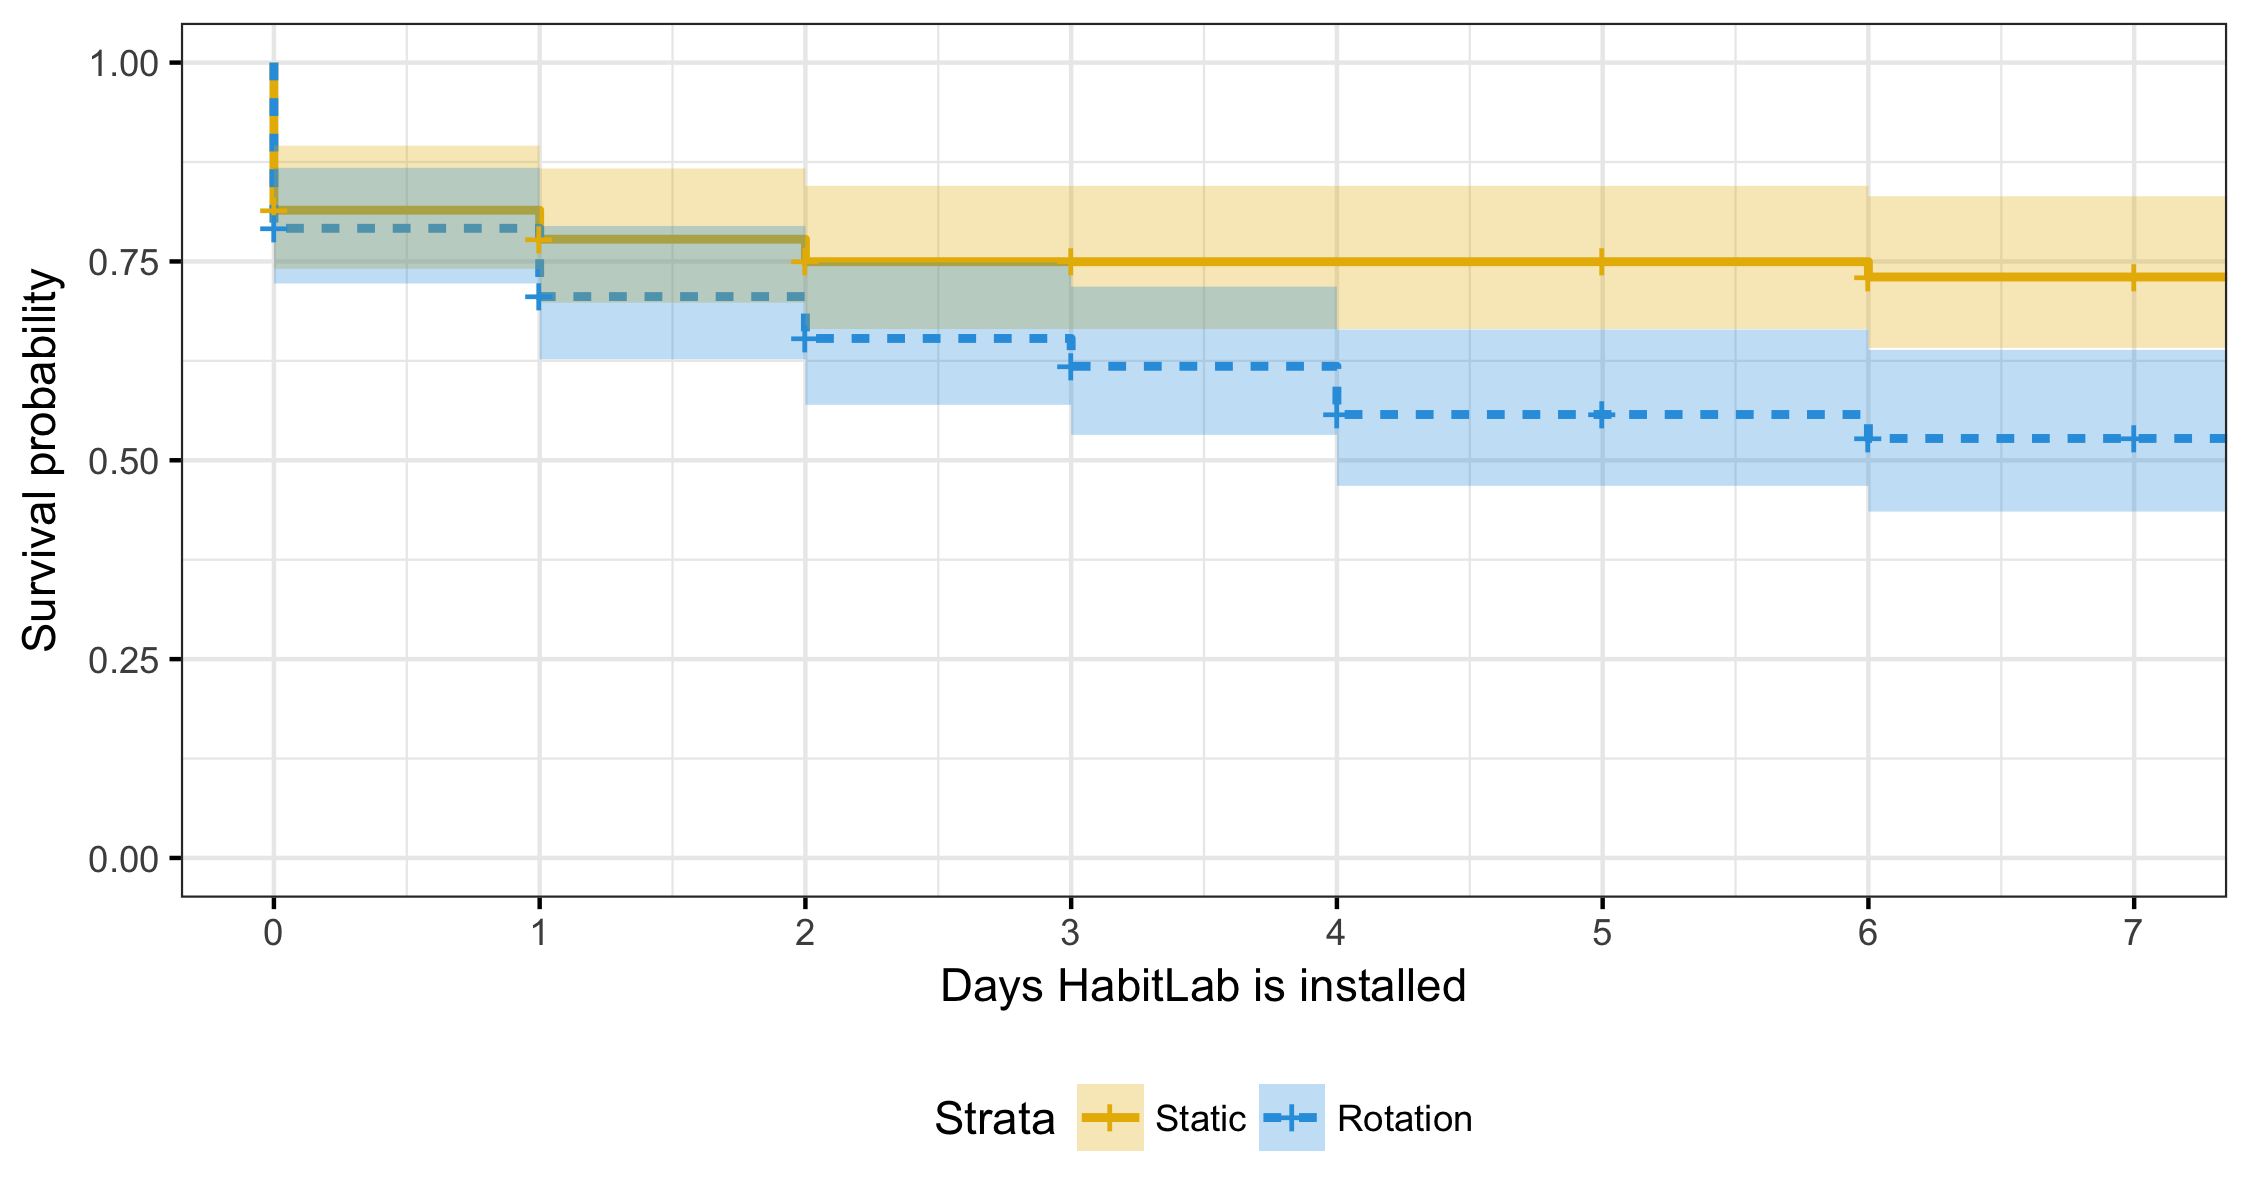
\includegraphics[width=1.0\textwidth]{figures/attrition_within_subjects.png}
	\caption{Rotating interventions increases attrition among users.}
\label{fig:attrition_within_subjects}
\end{figure}

% Table created by stargazer v.5.2 by Marek Hlavac, Harvard University. E-mail: hlavac at fas.harvard.edu
% Date and time: Thu, Apr 19, 2018 - 09:04:52
\begin{table}[tb] \centering 
  \caption{A Cox proportional hazards analysis suggests that the rotation condition substantially increases the hazard of attrition. Coefficients are log hazard ratio, so positive values indicate increased hazard and negative values indicate decreased hazard.} 
  \label{tab:cox_regression} 
\begin{tabular}{@{\extracolsep{5pt}}lc} 
\\[-1.8ex]\hline 
\hline \\[-1.8ex] 
 & \multicolumn{1}{c}{\textit{Dependent variable:}} \\ 
\cline{2-2} 
\\[-1.8ex] & Log hazard ratio \\ 
\hline \\[-1.8ex] 
 Rotation (baseline: static) & 0.544$^{*}$ \\ 
  & (0.249) \\ 
 \hline \\[-1.8ex] 
Observations & 217 \\ 
\hline 
\hline \\[-1.8ex] 
\textit{Note:}  & \multicolumn{1}{r}{$^{*}$p$<$0.05; $^{**}$p$<$0.01; $^{***}$p$<$0.001} \\ 
\end{tabular} 
\end{table} 

% (this is from the within-subjects study)

The Cox proportional hazard regression model comparing the static and rotation conditions found that attrition rates are significantly higher with the rotation condition (Figure~\ref{fig:attrition_within_subjects}, Table~\ref{tab:cox_regression}). After 2 days, 78\% of users remain in the static condition, while only 71\% remain in the rotation condition. After 7 days -- the duration of the longest experiment block -- 68\% of users remain in the static condition, while only 39\% of users remain in the rotation condition. These results support H\ref*{hyp:attrition}.

\rev{We considered the possibility that switching between static and rotated interventions contributes to attrition beyond simply rotating them. We analyzed this by comparing the probability of attrition on days where the condition remains the same as the previous day, to days where the condition changes -- either from static to rotated, or from rotated to static. The baseline daily attrition rate is 18\% when staying within the same experimental condition -- 14\% when staying within the static condition, and 20\% when staying within the rotation condition. On the first day after switching from static interventions to rotated interventions, the attrition rate is 36\% -- a significant increase compared to remaining within the same condition (Fisher's exact test, $p < 0.001$). However, switching from rotated interventions to static interventions does not increase the attrition rate -- it remains at 18\%. So we believe these effects are not due to the changes between conditions, but due to the conditions themselves --- switching from static to rotated is experiencing the first instance of a rotation, and it is not surprising that the effect may be larger with the first change.}

% (Fisher's exact test, p=0.0006)

%\subsection{Limitations}

%\geza{A limitation of Study 1 is that we cannot conclude with certainty where the cause of the increased effectiveness is from. Is it caused by benefits from the rotation itself? Or might it a side effect of selective attrition -- perhaps users for whom interventions are less effective, happen to be more susceptible to attrition if we are rotating intervention?}

%\geza{An additional limitation is that due to the short durations of our experimental blocks -- with the longest continual condition lasting only 7 days -- we could not observe long-term trends with respect to attrition and effectiveness.}

%TODO change these results to say that attrition is higher when showing random interventions

%There is no significant difference in rates of attrition between days on which users are shown random interventions vs always seeing the same one.

%Because attrition is a binary response variable rather than a normal distribution, we use a Generalized Linear Mixed Model with a binomial family for this analysis.

%We used a chi-squared test to compare the following two generalized linear mixed models for predicting whether or not the user attritions that day:

%Full model: condition ("same" or "random") [fixed effect], user [random effect]

%Reduced model: user [random effect]

%The condition did not significantly affect whether or not the user attritions that day ($\chi^{2}(1)$ = 0.4624, p = 0.4965) %, with condition=same increasing it by an estimate of 0.7549 (standard error 0.2982, t-value = 2.532) from an intercept of 5.3903.


%results <- glmer(attritioned ~ as.factor(condition) + (1|install_id), data = datadays_facebook, family='binomial')
%resultsnull <- glmer(attritioned ~ (1|install_id), data = datadays_facebook, family='binomial')

%results: attritioned ~ as.factor(condition) + (1 | install_id)
%            Df    AIC    BIC  logLik deviance  Chisq Chi Df Pr(>Chisq)
%resultsnull  2 70.896 76.046 -33.448   66.896                         
%results      3 72.434 80.158 -33.217   66.434 0.4624      1     0.4965

% Fixed effects:
%                         Estimate Std. Error z value Pr(>|z|)    
% (Intercept)                -9.717      2.149  -4.521 6.15e-06 ***
% as.factor(condition)same    1.291      1.951   0.662    0.508    

% https://stats.idre.ucla.edu/r/dae/mixed-effects-logistic-regression/

% https://stats.idre.ucla.edu/other/mult-pkg/introduction-to-generalized-linear-mixed-models/

% http://lme4.r-forge.r-project.org/slides/2011-01-11-Madison/5GLMM.pdf

%results <- lmer(attritioned ~ as.factor(condition) + (1|install_id), data = datadays_facebook)
%resultsnull <- lmer(attritioned ~ (1|install_id), data = datadays_facebook)



\section{Study 2: Longer-Term Effects of Rotation on Attrition}

% Study 1 found that compared to static interventions, rotation increases effectiveness but also increases attrition. To provide additional support for our findings in Study 1 and motivate our design experiment, we will now present a second field study that compared the effects of the amount of rotation on attrition rates. This study seeks to answer the question: Does the number of interventions in the rotation affect the level of attrition? In other words, is the effect due to the sheer existence of rotation, or is the number of alternatives important?
%\item Is user control over the interventions included in rotation associated with attrition rates?
%\end{enumerate}

% This second study occurs over a longer period than Study 1---ten weeks---allowing us to examine these effects in a more longitudinal setting.

Study 1 found that compared to static interventions, rotation increases effectiveness but also increases attrition. To provide additional support for our findings in Study 1 and motivate our design experiment, we present a second field study that seeks to answer the question: Does the number of interventions in the rotation affect the level of attrition? This study occurs over a longer period --- ten weeks --- allowing us to examine these effects in a more longitudinal setting.

\subsection{Participants}

% started Jan 24
% ended Feb 26

Our participants were HabitLab users who installed over a 5 week period in January--February 2018 and consented to our experiment protocol. 680 users who agreed to participate. After excluding users with multiple devices, users who did not complete the onboarding process, and users who had less than two sessions on Facebook where they saw interventions --- we restricted analysis in this study to users who were using Facebook because it had the most number of default interventions available --- we were left with 409 participants. Demographics were similar to Study 1.

\subsection{Method}

This was a between-subjects study where users' default settings for the number of enabled interventions varied depending on their condition: some users only had one default enabled intervention, and others had more. Interventions were then selected randomly from the enabled set. Among users who did not change these defaults, this enabled a between-subjects comparison of the effects of the number of interventions a user was rotating between, on retention rates.

% 163/225=0.7244444444444444 changed interventions for one condition
% 138/211=0.6540284360189573 changed interventions for half condition
% 137/200=0.685 changed interventions for all condition

In practice, we found that many users changed the set of interventions --- 78\% of participants in this study changed them over the course of using HabitLab, most often during onboarding. We wanted to retain a good user experience, but this muddied the experimental manipulation. So, we restricted analysis to the 91 users who did not change defaults. A $\chi^2$ test found there was no significant effect of condition on whether users changed defaults ($\chi^2(2)$= 0.4671, p=0.8), suggesting that randomization remained effective even after this filter.

% 72\% changed defaults in the one default condition, 65\% changed defaults in the half defaults condition, and 69\% changed defaults in the all defaults condition -- a chi squared test found there was no significant difference between categories for whether users changed defaults or not (chisquared= 0.4671, p=0.8). % (chisquared= 0.4671, p=0.791723) %\msb{The regression output says $N=91$. See \ref{tab:cox_regression_between_participants}. Where did the other people go?} \gezacomment{91 did not change ever, 117 did not change within the first 5 minutes}

Unlike Study 1, this was a between subjects experiment, so there were no time blocks: participants were assigned to the condition for the duration of the study.

\subsection{Conditions}
Participants were randomized into three conditions. In the one intervention condition, for every site the user enabled HabitLab on, only one intervention was enabled by default. The intervention was randomly chosen among the set of default interventions for that site. This is equivalent to the static condition from Study 1.

In the all interventions condition, for every site the user enabled, all interventions that are default for that site were enabled by default. This is equivalent to the rotation condition from Study 1. In the half interventions condition, for every site the user enabled, half of all interventions that are default for that site were enabled by default. The subset was chosen randomly.

\subsection{Measures}

We measured attrition, using the same procedures as those described in Study 1.

\subsection{Method of Analysis}

Like Study 1, we applied a Cox proportional hazards regression model to compare attrition rates.


\subsection{Results}

In this study, participants had an average of 3.3 target sites enabled. They visited at least one target site 64\% of days on average. On each of those days, participants experienced interventions an average of 6.8 times.

%\subsection{RQ3 (revisited): Does randomizing which interventions are shown each visit have any effects on attrition, compared to always showing the same one?}

\begin{figure}
\centering
	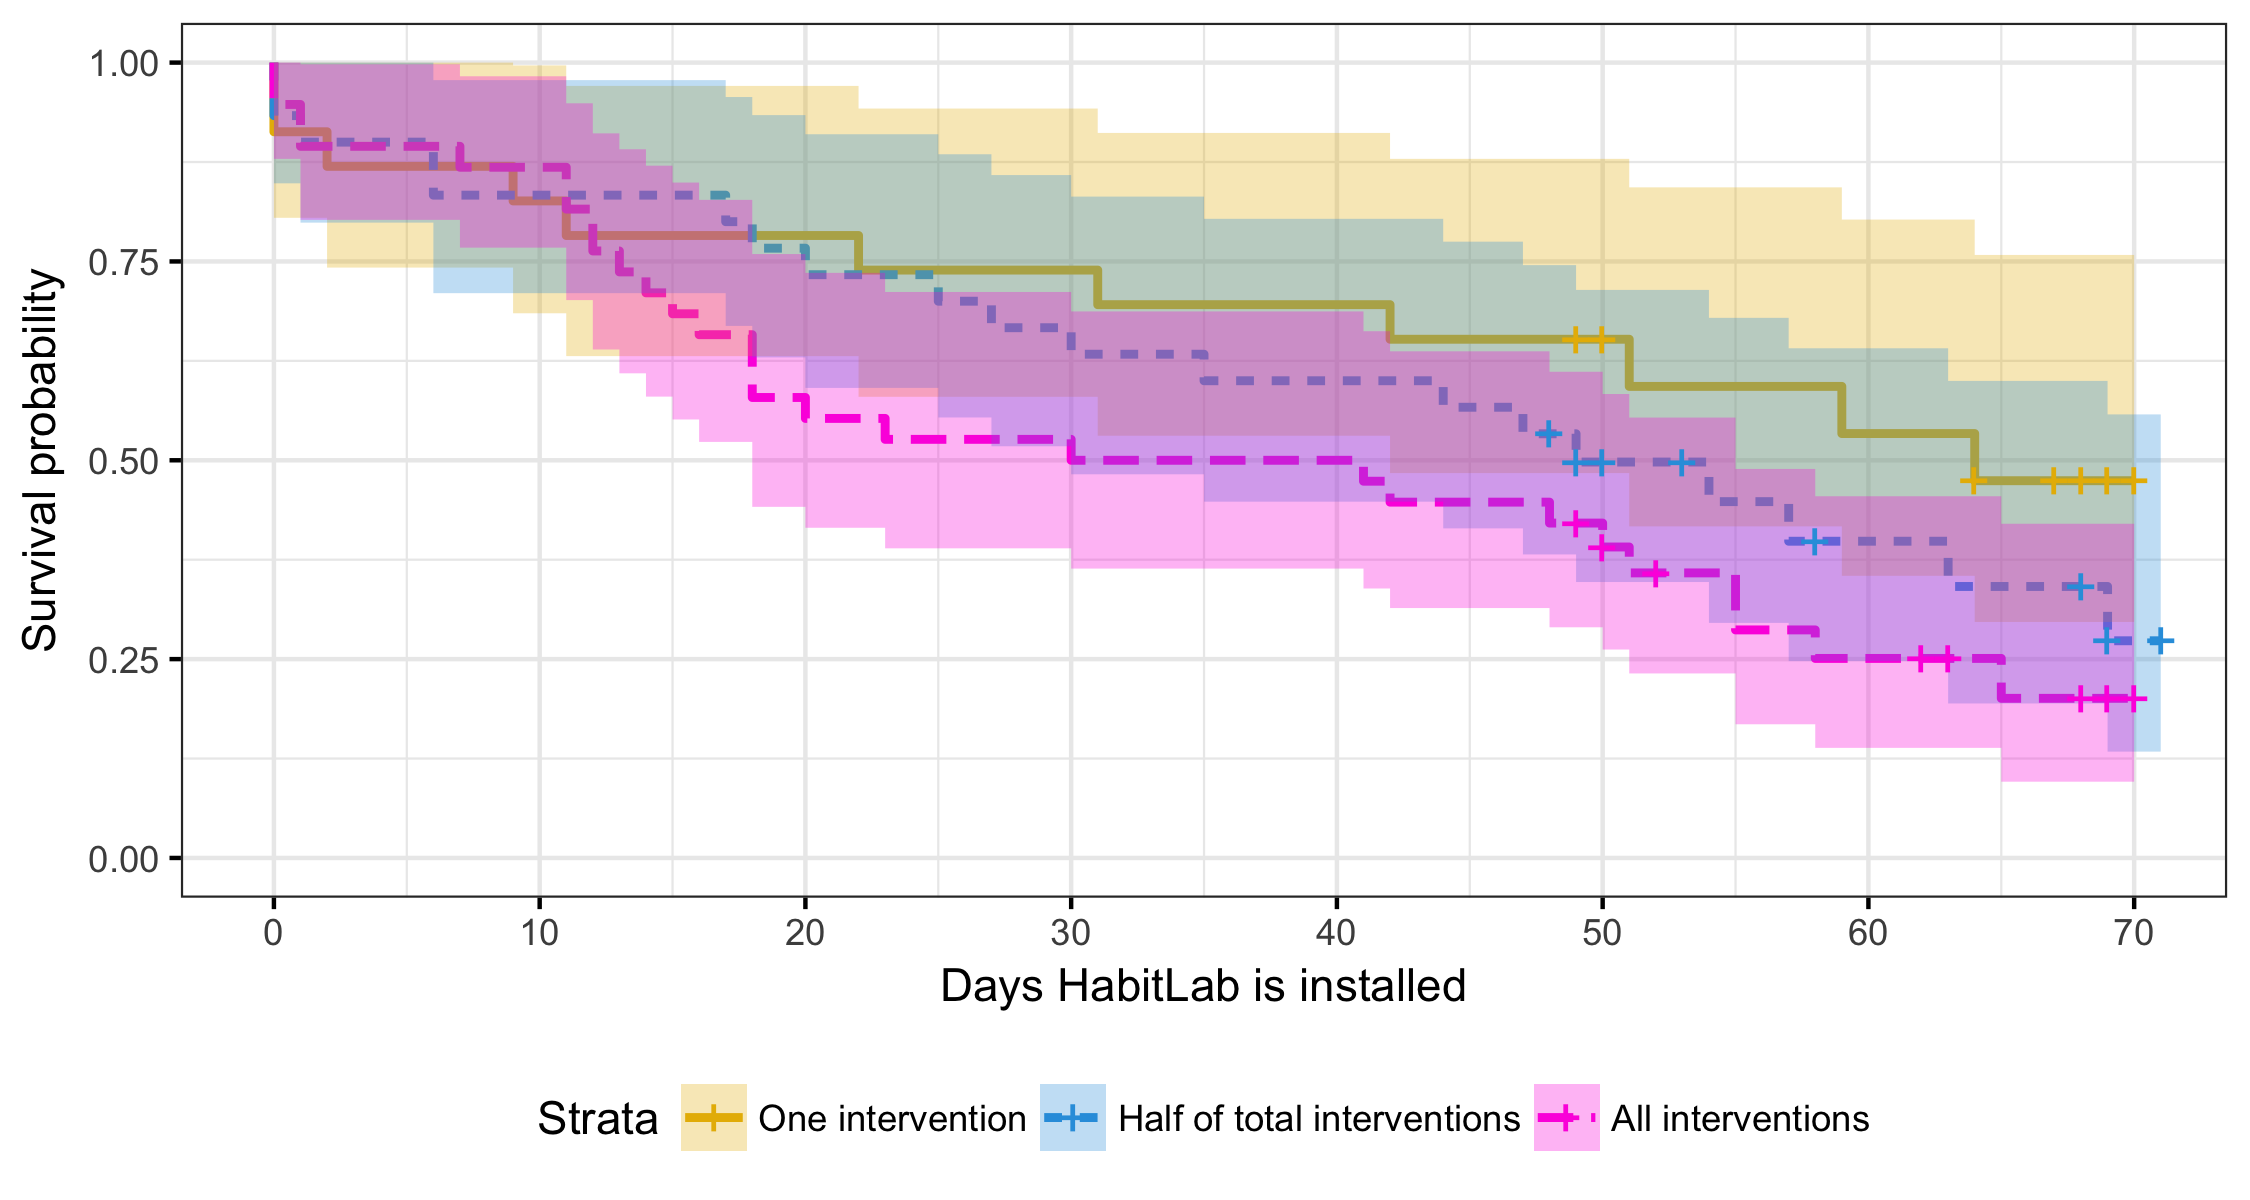
\includegraphics[width=1.0\textwidth]{figures/attrition_between_subjects.png}
	\caption{Including all interventions resulted in significantly more attrition than just one intervention.}
\label{fig:attrition_between_subjects}
\end{figure}

% Table created by stargazer v.5.2 by Marek Hlavac, Harvard University. E-mail: hlavac at fas.harvard.edu
% Date and time: Thu, Apr 19, 2018 - 09:01:42
\begin{table}[tb] \centering 
  \caption{A Cox proportional hazards analysis over a longer period suggests that rotating with more interventions increases the hazard of attrition.} 
  \label{tab:cox_regression_between_participants} 
\begin{tabular}{@{\extracolsep{5pt}}lc} 
\\[-1.8ex]\hline 
\hline \\[-1.8ex] 
 & \multicolumn{1}{c}{\textit{Dependent variable:}} \\ 
\cline{2-2} 
\\[-1.8ex] & Log hazard ratio \\ 
\hline \\[-1.8ex] 
 Half of total interventions (baseline: one intervention) & 0.395 \\ 
  & (0.380) \\ 
  All interventions & 0.711$^{*}$ \\ 
  & (0.358) \\ 
 \hline \\[-1.8ex] 
Observations & 91 \\ 
\hline 
\hline \\[-1.8ex] 
\textit{Note:}  & \multicolumn{1}{r}{$^{*}$p$<$0.05; $^{**}$p$<$0.01; $^{***}$p$<$0.001} \\ 
\end{tabular} 
\end{table} 

% (this is from the between-subjects study)

%We restricted our analysis to users who kept the default interventions during the first 5 minutes -- the same result can be obtained if we restrict our analysis to users who kept the default interventions during the entire period. Thus, the ``all defaults'' condition becomes equivalent to the ``rotation'' condition from Study 1, and the ``one default'' condition becomes equivalent to the ``static'' condition from Study 1.

In this longer, between-subjects experiment, attrition rates were significantly higher in the all interventions condition (Figure~\ref{fig:attrition_between_subjects}, Table~\ref{tab:cox_regression_between_participants}). This agrees with the analogous result from Study 1 showing a higher attrition rate for the rotation condition. The half of total interventions survival curve falls in between that of the one intervention and all interventions conditions, but does not have a statistically significant difference.

% \rev{What is the range of attrition rates between conditions? We can estimate a lower bound on attrition rate by looking at the subgroup with the lowest attrition. The group with the lowest attrition in the single intervention condition of this study were users in the one intervention condition whose only intervention was X. This had a retention rate of N\% over the course of M weeks.}

\begin{comment}
\subsection{RQ4: Are users who enable or disable interventions during onboarding less likely to attrition?}

%(this is actually from the between-subjects study)

\begin{figure}
\centering
	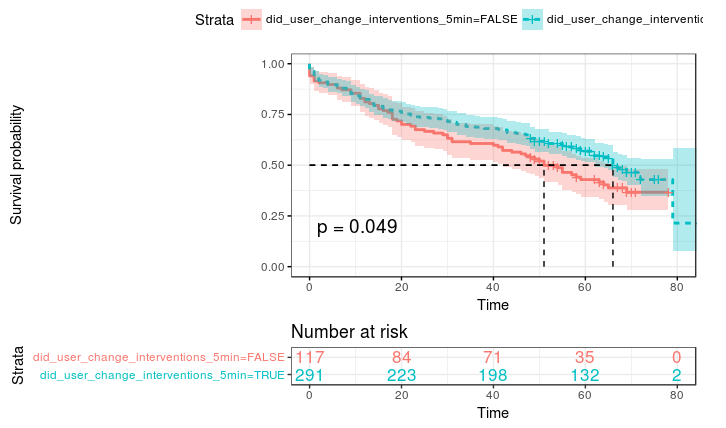
\includegraphics[width=1.0\textwidth]{figures/attrition_between_changed_interventions.png}
	\caption{Users who change interventions during the first 5 minutes will be significantly less likely to attrition later.}
\label{fig:attrition_between_changed_interventions}
\end{figure}

We compared users who enabled or disabled interventions during the first 5 minutes, compared to other users who completed the onboarding process without enabling or disabling any interventions. We found that users who enabled or disabled interventions during the first 5 minutes had a significantly lower rate of attrition, as shown in Figure~\ref{fig:attrition_between_changed_interventions}.



% \msb{TODO: what can we not generalize, given the design of our experiment and measures?}

\end{comment}

\section{Study 3: Design Interventions to Reduce Attrition}

Study 1 and Study 2 collectively demonstrated that rotation increases effectiveness but also increases attrition. Why does rotation increase attrition? To understand this, we needed to understand why users uninstalled in the first place.

We performed a qualitative content analysis on the uninstall feedback left to us by users. This feedback was collected in a tab that opened automatically when users uninstalled HabitLab. The page stated that feedback would be used for research purposes. Users had the option to check boxes to agree with a set of predefined reasons they why they were uninstalling, and leave free-text feedback. We performed an inductive analysis of the free-text feedback, grouping responses by themes, reflecting on our themes, and refining our groupings until convergence.

% 43 of the users who submitted the form were exposed to one of the conditions of study 1
% 101 of the users who submitted the form were exposed to one of the conditions of study 2

% A total of 782 users have submitted the uninstall feedback form over the course of HabitLab's deployment. This includes 8 participants from Study 1, and 39 from Study 2.
% https://v2.overleaf.com/17562771pkwbxzxyvtvv
A total of 782 users submitted the uninstall feedback form. This data represents all past users of HabitLab, and includes users outside studies 1 and 2. We use this larger dataset because only 8 participants from Study 1, and 39 from Study 2, filled out the feedback form. 751 users who submitted the form checked at least one of our predefined reasons. 274 users (36\%) uninstalled because ``Interventions were annoying'', 248 users (33\%) uninstalled because HabitLab ``Did not feel effective'', 100 users (13\%) uninstalled because HabitLab ``Was causing lag'', 75 (10\%) uninstalled due to ``Privacy concerns'', and 202 (27\%) cited ``Other reasons''. The total sums to more than 100\% because users could check more than one reason.

A total 155 users submitted free-form textual feedback. Some users began with an incorrect mental model and uninstalled after they learned what it was doing:
\begin{itemize}
%\item \textit{does not f***ing work, hiding the newsfeed in particular} [The ``hide news feed'' intervention was advertised on the HabitLab Chrome store page, but HabitLab never hit that intervention in its rotation for this user before they uninstalled]
\item \textit{Didn't seem what I was expected. Installed two minutes ago and removed it}
\item \textit{I just didn't understand the concept before downloading} %and it's [sic] intentions aren't my demons as it happens}
\end{itemize}

Some users indicated they wanted more control over the intervention that was shown to them, or were simply looking for a time tracker and were not interested in interventions at all:
\begin{itemize}
\item \textit{I wanted a timer for every ``domain'', it can be good for statistics of time}
\item \textit{I was interested in tracking my usage to start, instead of setting interventions that I may not actually be concerned about}
% \item \textit{Would have preferred a gentle log - perhaps emailed - giving usage statistics. In present form this operates like pop-up ads. Still, it was reasonably insightful into understanding my usage for the time I used it}
\end{itemize}

Some users indicated dissatisfaction with particular interventions:
\begin{itemize}
\item \textit{Mostly it was the bar covering up facebook message indicators}
%\item \textit{You covered up useful buttons. Don't do that}
% \item \textit{Made Facebook unusable. Which might be the point?}
\item \textit{it was just annoying you out of not using sites, not convincing you to. It became like ads, they are always there. But you don't like them and turn them off with ad-block.}

\end{itemize}

Some users wished interventions would be more forceful, or less intrusive:
\begin{itemize}
\item \textit{Interventions are not forceful enough. They are too easy to click around or disable}
% \item \textit{Looked like some nice options for streamlining sites, but it's actually a nanny. I don't need a nanny whining at me.}
\item \textit{I liked the interventions but not on every page change or load, that was just a bit too much}
\end{itemize}

Finally, some users decided they simply did not want or need interventions:
\begin{itemize}
\item \textit{Made me realize I don't have Facebook addiction, spending less than 30 minutes [...] per day} %of my desktop time on it per day}
\item \textit{I'm weak...}
\end{itemize}


Other themes included localization issues, performance issues, privacy concerns, accidental installations, and misattribution of other issues to HabitLab.

\begin{comment}
Some feedback indicated that users had an incorrect mental model of the system: they were expecting to see a particular intervention consistently, instead of having them rotate:

\textit{does not fucking work, hiding the newsfeed in particular}

Other users began with an incorrect mental model and uninstalled after they learned what it was doing:

\textit{Didn't seem what I was expected. Installed two minutes ago and removed it}

\textit{I just didn't understand the concept before downloading and it's intentions aren't my demons as it happens}

Some users indicated they wanted more control over the intervention that was shown to them, or were simply looking for a time tracker and were not interested in interventions at all:

\textit{I wanted a timer for every "domain", it can be good for statistics of time}

\textit{I was interested in tracking my usage to start, instead of setting interventions that I may not actually be concerned about}

\textit{Would have preferred a gentle log - perhaps emailed - giving usage statistics. In present form this operates like pop-up ads. Still, it was reasonably insightful into understanding my usage for the time I used it}

Some users indicated dissatisfaction with particular interventions:

\textit{Mostly it was the bar covering up facebook message indicators}

\textit{You covered up useful buttons. Don't do that}

\textit{Made Facebook unusable. Which might be the point?}

%``There was a very irritating bug with Klout''

Some users wished interventions would be more forceful:

\textit{Interventions are not forceful enough. They are too easy to click around or disable}

Some users were getting fatigued from seeing too many interventions:

\textit{Looked like some nice options for streamlining sites, but it's actually a nanny. I don't need a nanny whining at me.}

\textit{I liked the interventions but not on every page change or load, that was just a bit too much}

\textit{it was just annoying you out of not using sites, not convincing you to. It became like ads, they are always there. But you don't like them and turn them off with ad-block.}

Some users disliked that the intervention was reminding them that they were visiting sites:

\textit{I noticed that I was going on imgur, youtube, facebook (my choice of addictive sites) more, after I had installed the extension. So, I'm uninstalling. I think the extension made me more conscious of the fact that I was visitng the sites, but maybe the rewards were making me go back to the site? I'm not sure}

%There were also users who may have had limited command of English (the user's locale was set to LANGUAGE), and may not have understood the text presented during onboarding because the app was not localized to their native language:

%``no like interference in all''

There were also users who cited localization issues, or may not have understood the text presented during onboarding because the app was not localized to their native language:

\textit{Translate in french please} -- This was from before we localized to French

\textit{non lo voglio} -- Italian for I don't want it. The extension is not localized to Italian

Some users cited performance issues, bugs, or conflicts with other extensions:

\textit{Was awesome, but was making chrome really slow, i mean really slow! Seems like you need to fix some memory issues}

\textit{It's quite possible something else was causing lag -- but lag was there. I also was just checking it out. I don't really use facebook or youtube}

\textit{Catastrophic stability problems after installation; may be due to a different extension}

\textit{Seeing if this extension is causing gmail compatibility issues}

\textit{Wasn't sure if it is effecting battery life}

Some users had simply been testing the app or evaluating alternatives:

\textit{I love the app - I'm just removing temporarily to see if it's affecting another app (Freedom.to)}

\textit{I want to try other types of chrome extensions to block time-consuming websites and don't want to mess with your data}

\textit{I prefer the "Forest" application}

\textit{I forgot that I already had another program that did essentially the same thing for the computer in general instead of just for this particular browser}

Some users had privacy concerns:

\textit{I was just worried, I mean it's (Anonymized) and all, but a bunch of students tracking everything I do and all my browser history, that just felt too much of a price to pay}

Finally, many uninstalls were simply due to the extension being automatically installed on a non-work computer due to Chrome's behavior of automatically installing extensions across all devices, which is why we had restricted analyses to just users who used one device:

\textit{Neighbor installed this to my computer without my consent!}

\textit{Someone else installed. Did not want it}

\textit{Dont need it on work computer, just at home}

\textit{this is my wasting time computer and i dont need it}

Some users decided they simply did not want or need interventions:

\textit{Made me realize I don't have Facebook addiction, spending less than 30 minutes of my desktop time on it per day}

\textit{I rarely waste time on my desktop. This would be much more useful on my mobile phone}

\textit{I just don't use my laptop as much as I thought would be necessary for an intervention}

%\textit{realized not spending as much time on websites as i thought...}

%\textit{I figured out that I actually don't spent as much time as I thought I was. I thought I was watching videos for 4 to 5 hours a day, but the timer stated only watch them for 30 minutes}

%\textit{I'm weak...}

Some users uninstalled due to misattributing other issues to our software:

\textit{For some reasons Facebook blocked me and I am trying to figure out the reasons. What I know that the Habitlab extension was deactivated (not by me) and then, boom, I was blocked}

Finally, some users reached their goals and decided they simply didn't need the extension anymore:

\textit{I reached my goal to reduce time spent on certain pages. Thanks folks!}

\textit{I used the extension to curb my Facebook habit and eventually gave up Facebook altogether - something I've been wanting to do for a long time. Thank you}

\end{comment}

\subsection{Design interventions}

Based on the qualitative feedback on reasons for uninstalling, we drew on two of the most consistent themes to hypothesize why rotation may be increasing attrition:

\begin{hyp}[H\ref*{hyp:mentalmodel}] \label{hyp:mentalmodel}
Violation of mental model: Users may have sped through onboarding and not understood that HabitLab rotates interventions. So, when they experience a new intervention, the system violates their mental model and they disable it in confusion or frustration.
\end{hyp}

\begin{hyp}[H\ref*{hyp:control}] \label{hyp:control}
User control: Users may be aware that the system is choosing interventions for them, but are frustrated by a lack of control over the system's behavior. They may dislike one or more of the interventions but not realize how to turn them off.
\end{hyp}

%\begin{enumerate}
%\item Violation of mental model: Users may have sped through onboarding and not understood that HabitLab rotates interventions. So, when they experience a new intervention, the system violates their mental model and they disable it in confusion or frustration.%Users may have an incorrect mental model expecting that interventions they see do not change. Even though we told them during onboarding that HabitLab will change interventions periodically, they may not have read it. % insert citation that violating user expectations results in attrition here
%\item Lack of control: Users may be aware that the system is choosing interventions for them, but are frustrated by a lack of control over the system's behavior. They may dislike one or more of the interventions. %uncomfortable giving control to a system % insert citation that control is good here
%\item Changes prompt a reminder to uninstall: If users grow blind to interventions over time, they may forget that it exists. This would lead to the observed result of decreased effectiveness and lower attrition.% never grow sufficiently annoyed to actually bother to uninstall. % insert citation that uninstalls are caused by annoying users
%\item Encountering bad interventions: Some users may have a particularly adverse reaction to some interventions -- simply seeing a certain intervention may lead the user to uninstall. For example, we found that users were on average over twice as likely to uninstall after a visit where they saw the intervention that closes the tab after 60 seconds, compared to the less intrusive interventions that showed time spent. By switching between several interventions, the user is more likely to encounter an intervention they have an intense dislike for. % insert citation that a bad intervention can cause an uninstall
%\end{enumerate}

These two hypotheses could feasibly be addressed through design interventions. \rev{Other pieces of feedback, for example how aggressive the interventions were, we judged as out of scope of the current study on rotation strategies and will pursue as future work.}  We developed two different interfaces, one to address mental model violation and the other to address a perceived lack of control. They are shown to users when they see a new intervention for the first time.

The first design, which we will call \textit{mental model} (Figure~\ref{fig:info}), is inspired by H\ref*{hyp:mentalmodel}: it reminds the user that HabitLab has rotated to a new intervention and gives the name of the intervention. If mental model misalignment was the issue, this design might help explain to the user what the system is doing and why. The second design, which we will call \textit{user control} (Figure~\ref{fig:power}), is inspired by H\ref*{hyp:control}: it includes the message in the information design but also adds a toggle option to allow the user to turn off the new intervention for future visits without needing to visit HabitLab's settings. If lack of control was the issue, this design may give sufficient control so that users keep HabitLab enabled. 

\begin{comment}
We hypothesized:
\begin{hyp}[H\ref*{hyp:design}] \label{hyp:design}
The information and control designs will have less attrition than a control design. 
\end{hyp}
\end{comment}

\begin{figure}
\begin{minipage}[t]{0.49\linewidth}
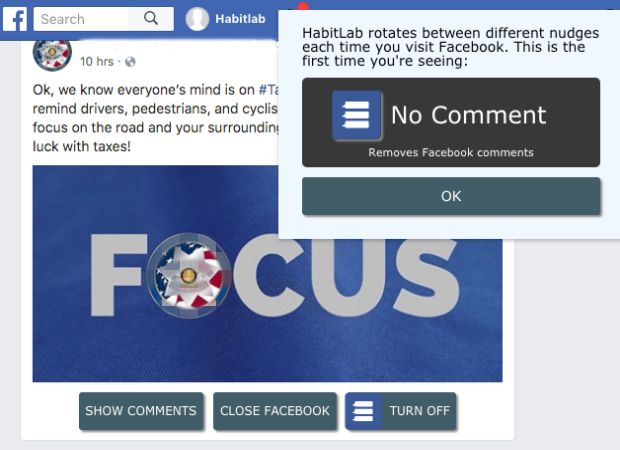
\includegraphics[width=\linewidth]{figures/info_full_facebook_new}
\caption{Mental model interface: each time the user sees a new intervention, HabitLab names it and explains about rotation.}
  \label{fig:info}
\end{minipage}
\hfill
\begin{minipage}[t]{0.49\linewidth}
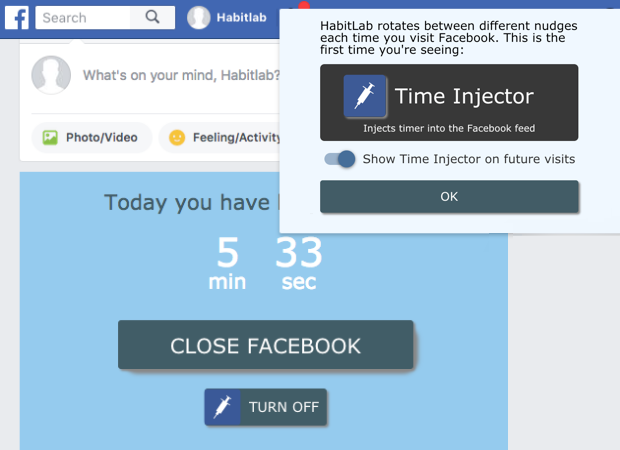
\includegraphics[width=\linewidth]{figures/power_full_facebook_new}
\caption{User control interface: in addition to the mental model information, HabitLab gives users a direct interface to disable the new intervention.}
  \label{fig:power}
\end{minipage}%
\end{figure}

%\subsection{Experimental Design}

% We ran a study comparing the ``info'' and ``power'' designs to our original system we had used in Study 1 (where the new intervention is shown without any additional messaging). An intervention was randomly selected on each visit -- the same configuration which we had found in Study 1 would increase attrition rates relative to always showing the same intervention.

\subsection{Experiment Design}

We ran a between-subjects design where we randomized the design shown to new users of HabitLab and tested whether it impacted attrition over a period of one week, similar to Study 1.

\subsection{Participants}

Our participants were HabitLab users who installed over a 10 day period in April 2018. There were a total of 282 users who installed and agreed to participate. We removed users who were not new users (e.g. an existing user installing on a new device, or a former user reinstalling the system), and users who left before they saw their first intervention. This leaves us with data from 93 participants. Demographics, estimated by Google Analytics, were similar to Study 1.

\subsection{Method}
Participants installed HabitLab and set it up as described in the Study 1 and Study 2. They used HabitLab in the course of their normal web browsing activity. HabitLab rotated between randomly chosen interventions on each visit to the chosen web page for all users, equivalent to the rotation condition in Study 1. Each time the user experienced a new intervention that they had not seen before, however, HabitLab might show an explanation design in the corner of the browser.

\subsection{Conditions}

There were three conditions for this study. %, one with no change from the last study and the other two with the new design interventions. 
%were interested in whether user retention rates would be influenced by whether or not users saw one of our two designs the first time they saw a new intervention.
%There were 3 conditions, which differ only in the design users see the first time they see a new intervention they have not previously seen. 
In the no design condition, users saw no message, equivalent to the rotation condition from Study 1. In the mental model condition, users were shown the informational intervention (Figure~\ref{fig:info}) to remind them that the system rotates interventions. In the user control condition, users were additionally given control over whether to turn off each new intervention without needing to visit the settings screen (Figure~\ref{fig:power}).

\subsection{Measures}

Our main dependent variable was attrition---how many days users kept the system installed by the end of the study, seven days after installation. The measure of attrition was the same as in Study 1 and Study 2. We also measured effectiveness, using the same method as Study 1.

\subsection{Method of Analysis}

To analyze attrition, we again used a Cox proportional hazards regression model, similar to Study 1, using interaction design as the predictor variable. To analyze effectiveness, we used a LMM predicting log time on site per day, with a fixed effect for condition, and random effects for participant and domain. Data cleaning followed the same procedures as Study 1.


%\section{Study 2 Methodology}

%Having observed in study 1 that there is an increase in attrition when alternating interventions, we sought to uncover the underlying causes. We hypothesized the following possible causes:

%\begin{enumerate}
%\item Violation of user expectations: Users may have an incorrect mental model expecting that interventions they see do not change. Even though we told them during onboarding that HabitLab will change interventions periodically, they may not have read it.
%\item Lack of control: Users may be aware that the system is choosing interventions for them, but are uncomfortable giving control to a system
%\item Seeing a new intervention reminds them that the system exists: If users grow blind to interventions over time, they may never grow sufficiently annoyed to actually bother to uninstall.
%\item Encountering bad interventions: Some users may have a particularly adverse reaction to some interventions -- simply seeing a certain intervention may lead the user to uninstall. By switching between several interventions, the user is more likely to encounter an intervention they have an intense dislike for.
%\end{enumerate}

%Reasons (3) and (4) are important -- and in fact we did observe a significant difference in attrition rates among different interventions in Study 1, confirming hypothesis (4) -- but are somewhat inevitable consequences of alternating between interventions. We also observed in informal in-person interviews that some users did not expect the system to be changing interventions. Thus, we chose to focus on addressing (1) and (2).

%We developed 2 different interfaces that aimed to address these possible violations of user expectations and provide users with a sense of control over their interventions. These interfaces were shown when users see a new intervention for the first time. The first interface, which we will call ``info'', shown in Figure \ref{fig:info}, tells the user that HabitLab rotates between different nudges. The second ``power'', shown in Figure \ref{fig:power}, shows the same message, and adds a toggle option to turn off the intervention for future visits.

%We ran a study comparing the ``info'' and ``power'' interventions to our original system we had used in Study 1 (where the new intervention is shown without any additional messaging). An intervention was randomly selected on each visit -- the same configuration which we had found in Study 1 would increase attrition rates relative to always showing the same intervention.

%\begin{figure}
%  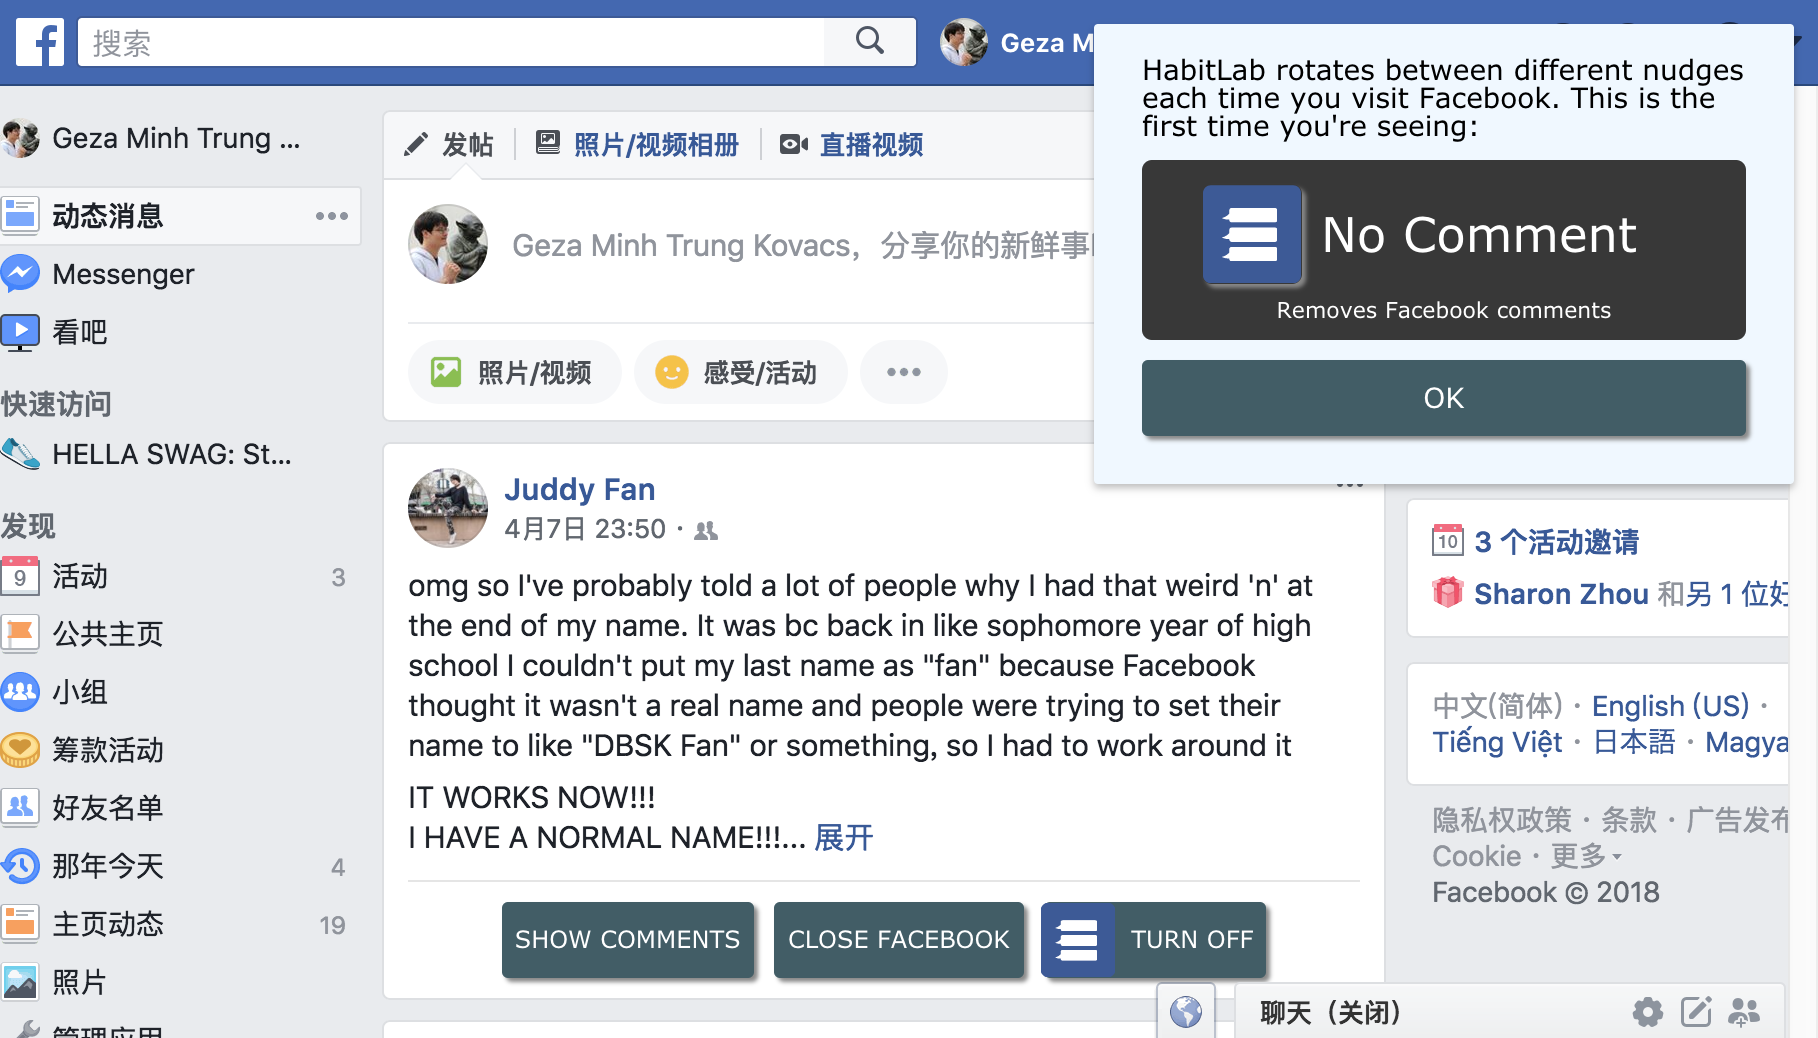
\includegraphics[width=\textwidth]{figures/info_full_facebook}
%  \caption{Interface showing info about how interventions alternate the first time a new intervention is seen.}
%  \label{fig:info}
%\end{figure}



%\begin{figure}
%  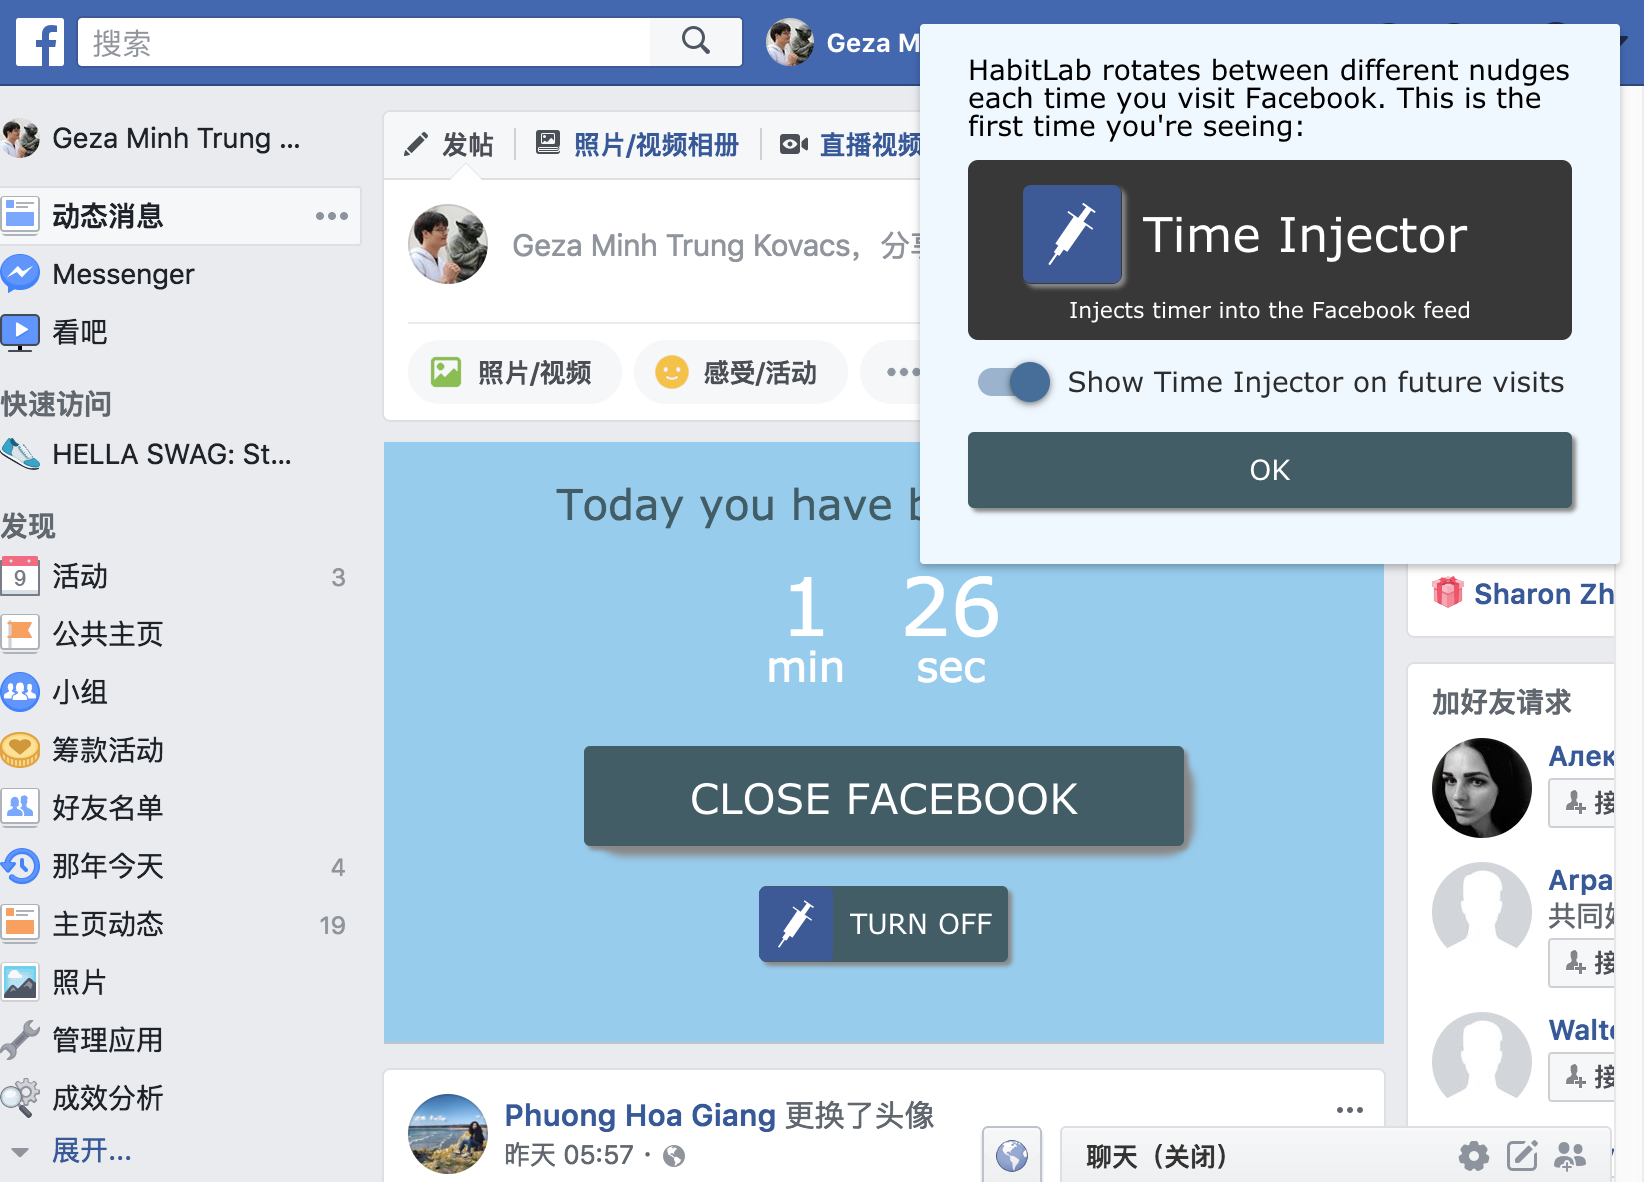
\includegraphics[width=\textwidth]{figures/power_full_facebook}
%  \caption{Interface giving users control over interventions the first time a new intervention is seen.}
%  \label{fig:power}
%\end{figure}



\subsection{Results}

In this study, participants had an average of 2.9 target sites enabled. They visited at least one target site 71\% of days on average. On each of those days, participants experienced interventions an average of 6.6 times.

% \subsection{RQ5: Does improving users' mental model by reminding them of how the system works when presenting a new intervention help reduce attrition?}

\begin{figure}[tb]
\centering
	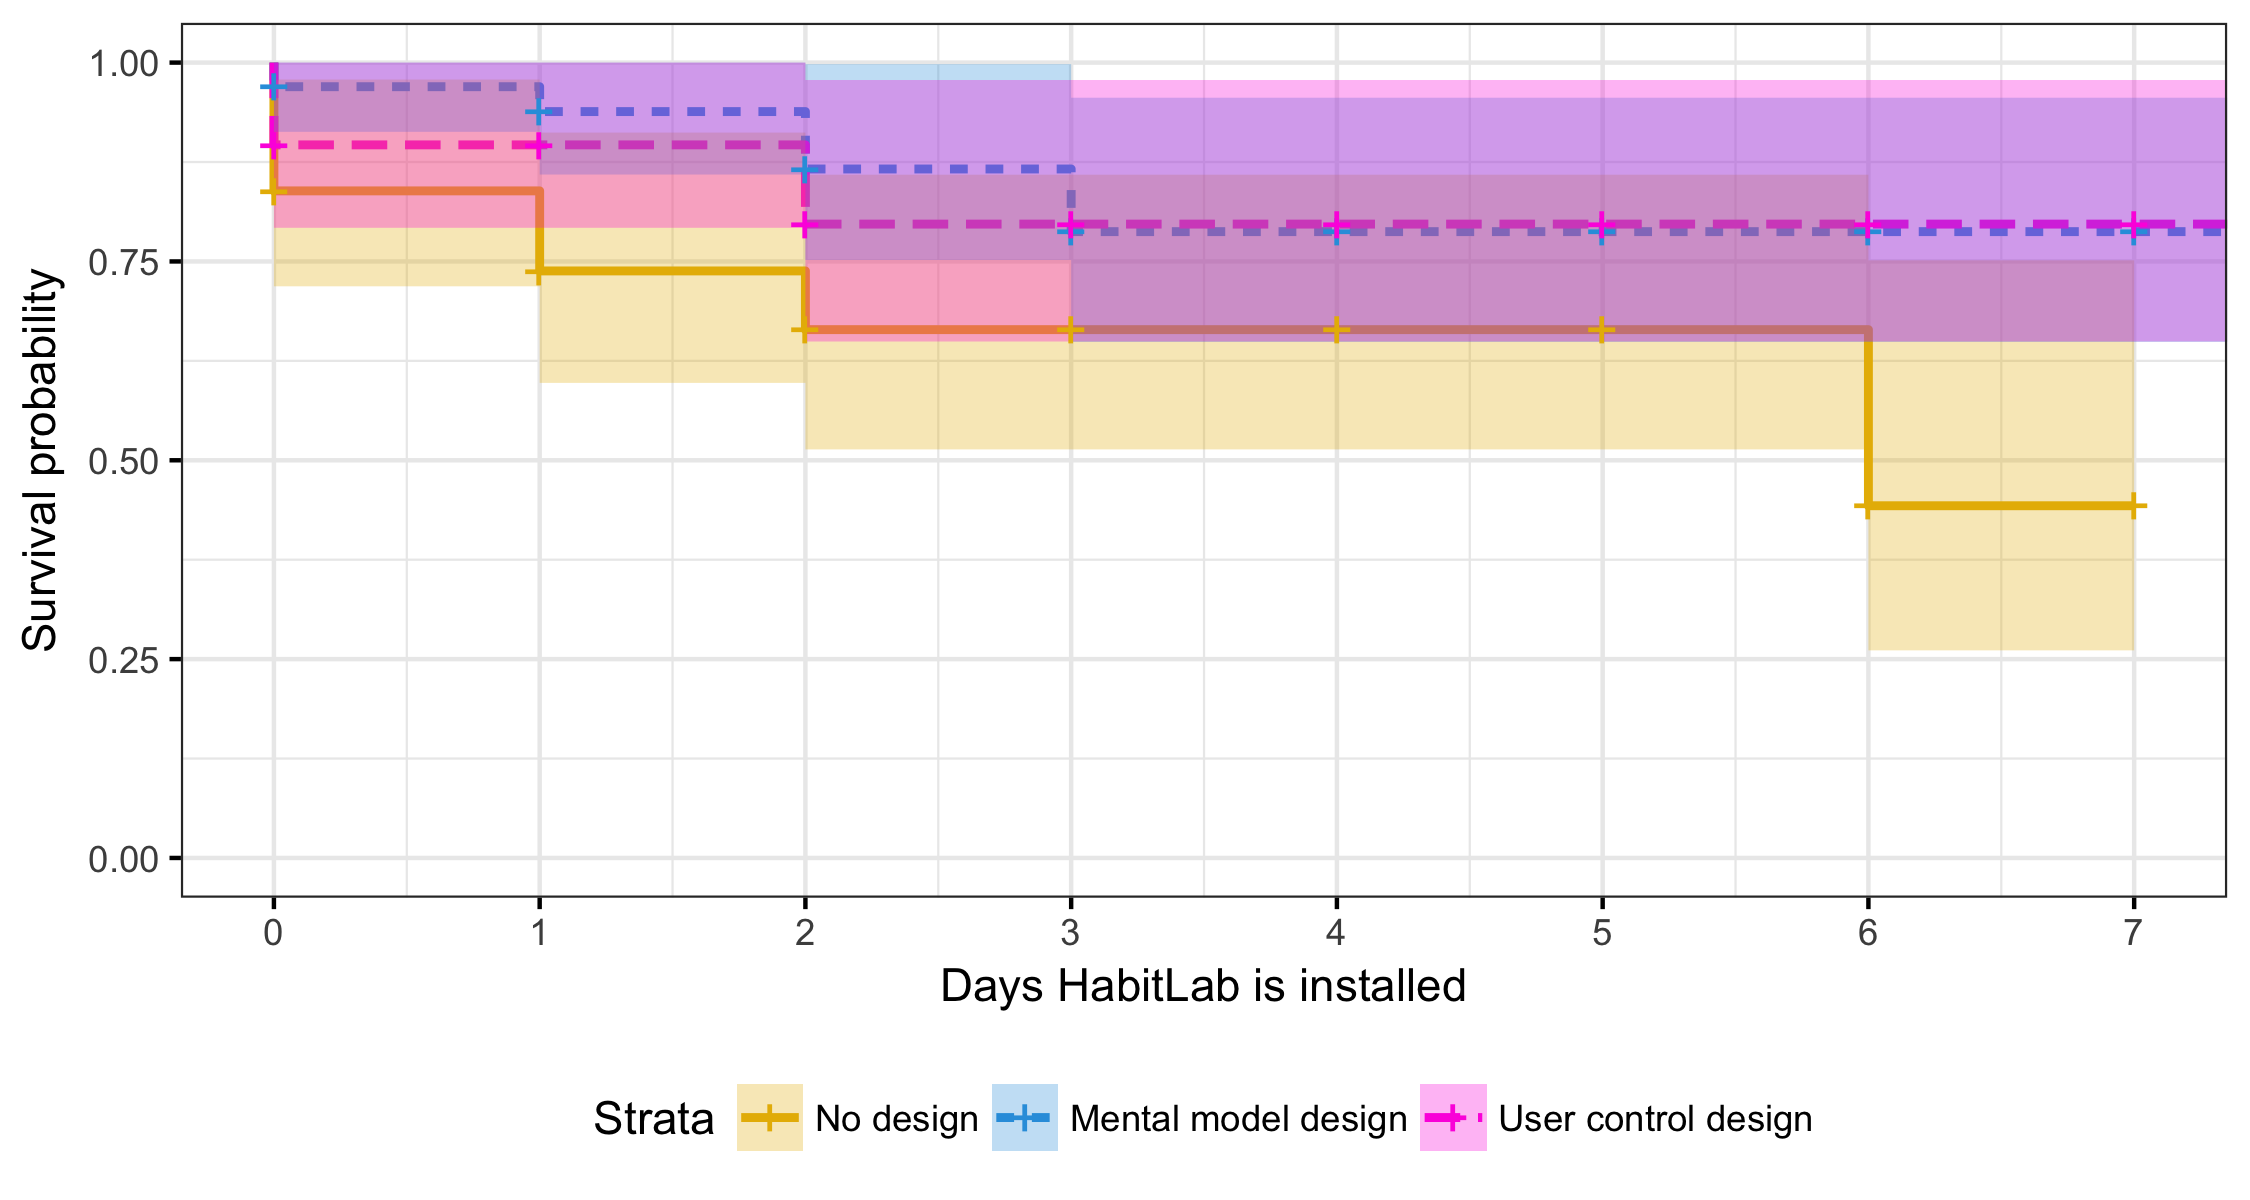
\includegraphics[width=1.0\textwidth]{figures/none_vs_info.png}
	\caption{Reminding users about how the rotations worked every time a new intervention was introduced significantly reduced attrition rates.}
\label{fig:attrition_none_vs_info}
\end{figure}

% Table created by stargazer v.5.2 by Marek Hlavac, Harvard University. E-mail: hlavac at fas.harvard.edu
% Date and time: Thu, Apr 19, 2018 - 09:03:30
\begin{table}[tb] \centering 
  \caption{A Cox proportional hazards analysis suggests that the informational intervention that corrected users' mental models was successful in reducing attrition due to rotation. Coefficients are log hazard ratio.} 
  \label{tab:cox_regression_design} 
\begin{tabular}{@{\extracolsep{5pt}}lc} 
\\[-1.8ex]\hline 
\hline \\[-1.8ex] 
 & \multicolumn{1}{c}{\textit{Dependent variable:}} \\ 
\cline{2-2} 
\\[-1.8ex] & Log hazard ratio \\ 
\hline \\[-1.8ex] 
 Mental model design & $-$1.015$^{*}$ \\ 
  & (0.494) \\ 
  User control design & $-$0.869 \\ 
  & (0.527) \\ 
 \hline \\[-1.8ex] 
Observations & 93 \\ 
\hline 
\hline \\[-1.8ex] 
\textit{Note:}  & \multicolumn{1}{r}{$^{*}$p$<$0.05; $^{**}$p$<$0.01; $^{***}$p$<$0.001} \\ 
\end{tabular} 
\end{table} 

% \subsection{RQ6: Does improving users' sense of control by allowing them to opt-out of seeing a newly introduced intervention in the future help reduce attrition?}

The Cox proportional hazard regression indicates that the mental model design  significantly reduces attrition rates relative to no design ($p < 0.05$, Figure~\ref{fig:attrition_none_vs_info}, Table~\ref{tab:cox_regression_design}). This result supports H\ref*{hyp:mentalmodel}. % After 2 days, 94\% of participants in the mental model condition remain, while 82\% remain in the user control condition and only 72\% remain in the no design (control) condition. Adding the additional option to permanently turn off the intervention the first time it is seen does not significantly change attrition rates, relative to simply informing the user that rotation is happening. % 7 days
After seven days, 79\% of participants in the mental model condition remain, while 80\% remain in the user control condition and only 44\% remain in the no design (control) condition. In other words, the intervention coditions more than halved the attrition rate, from 56\% to 21\% attrition. Adding the additional option to permanently turn off the intervention the first time it is seen is not significantly different from no design given our sample size. % It appeared to perform similarly to the mental model condition (Figure~\ref{fig:attrition_none_vs_info}), but had larger variance, thus the lack of statistical significance. This result indicates that H\ref*{hyp:control} was not supported.

There was no effect of condition on effectiveness: the full model was not significantly more explanatory than the reduced model without the condition variable ($\chi^{2}(2) = 1.46, n.s.$). So, these interventions did not reduce effectiveness while they were improving attrition. %Showing the designs had no effect on daily time spent per domain, using the same analysis from Study 1, as shown in Table~\ref{tab:designs_timespent_noeffect}. % 7 days

% In sum, adding an information intervention reduced attrition by more than a half, from 56\% to 21\% attrition. % \msb{TODO: change all these numbers to seven days, to match the graphs} \geza{done}

% \msb{TODO: support or not support H4, H5}

% \msb{TODO: ideally, report whether the interventions impacted effectiveness} \gezacomment{done}

% Table created by stargazer v.5.2 by Marek Hlavac, Harvard University. E-mail: hlavac at fas.harvard.edu
% Date and time: 三, 4月 18, 2018 - 22时28分14秒
% \begin{table}[tb] \centering 
%   \caption{Daily time spent on sites in the no design, mental model, and user control conditions. There was no significant difference in time spent between conditions.} 
%   \label{tab:designs_timespent_noeffect} 
% \begin{tabular}{@{\extracolsep{5pt}}lc} 
% \\[-1.8ex]\hline 
% \hline \\[-1.8ex] 
%  & \multicolumn{1}{c}{\textit{Dependent variable:}} \\ 
% \cline{2-2} 
% \\[-1.8ex] & Log time spent per day \\ 
% \hline \\[-1.8ex] 
%  Mental model (baseline: no design) & $-$0.170 \\ 
%   & (0.191) \\ 
%   User control & 0.042 \\ 
%   & (0.186) \\ 
%   Constant & 4.554$^{***}$ \\ 
%   & (0.198) \\ 
%  \hline \\[-1.8ex] 
% Observations & 1,041 \\ 
% \hline 
% \hline \\[-1.8ex] 
% \textit{Note:}  & \multicolumn{1}{r}{$^{*}$p$<$0.05; $^{**}$p$<$0.01; $^{***}$p$<$0.001} \\ 
% \end{tabular} 
% \end{table} 

% \begin{figure}[tb]
% \centering
% 	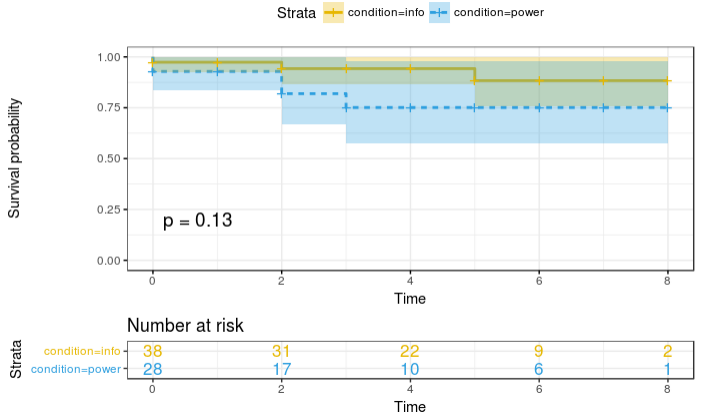
\includegraphics[width=1.0\textwidth]{figures/info_vs_power.png}
% 	\caption{Adding an option to permanently turn off the intervention to our design did not change attrition rates relative to simply showing information.}
% \label{fig:attrition_info_vs_power}
% \end{figure}



\section{Discussion}

%\msb{This section needs more meat}

Our findings suggest that changing behavioral interventions can be beneficial from the perspective of efficacy, but detrimental to retention. By showing simple messages when presenting new interventions, we can improve users' mental models, and reduce attrition from changing interventions.

In addition to the interface-based techniques we have presented to combat detrimental effects of changing interventions, algorithmic techniques can also help. For example, in the context of a multi-armed bandit, potential algorithmic techniques include:

\begin{enumerate}
\item Limiting the exploration speed such that users are not overwhelmed by the rate at which they are seeing new interventions.
\item Modeling individual interventions' likelihood of attrition, and favoring algorithms which are less likely to cause attrition if needed to keep the user around longer.
\end{enumerate}

There are also additional interface-based techniques that may be helpful in reducing attrition from changing interventions, but that we have not tested, such as:

\begin{enumerate}
\item Making how new interventions are introduced predictable and known to the user.
\item Allowing users a choice of intervention when we introduce new interventions.
\end{enumerate}



\subsection{Limitations}
This work featured deployment periods of a few weeks.  This may not be enough time to observe some very long-term effects: for example, some changes in intervention effectiveness set in only after months or years \cite{krebs2010meta}. That said, given the fast turnover rate which is observed with behavior-change software, even short-term effects of changing interventions on attrition can be important.

While we believe our general finding about the double-edged nature of changing interventions may apply to other behavior-change contexts, particular parameters---such as speed at which users grow blind to an intervention, may be domain-specific.

One shortcoming of our Study 1 design is that we cannot rule out the possibility that our observed increase in effectiveness is due to selective attrition, rather than due to benefits from the rotation. Namely, it is possible that observing rotation may selectively lead to uninstallation for users for whom interventions are ineffective. To rule out this possibility, we will need to investigate ways to maintain retention in the presence of rotation, and see whether the improvement in effectiveness relative to a static intervention still remains. It may also be possible to design intention-to-treat analyses that discount attrition in measures of effectiveness. \rev{Furthermore, while we observed that the first visit is longer than subsequent visits when users visit sites multiple times per day, but this effect may be due to temporal usage patterns rather than intervention effectiveness}.

% The nature of the HabitLab platform---using organic, real-world users for research---imposes constraints on the types of qualitative work we can do. As evidenced by the number of users who uninstall before even seeing their first intervention, real-world users have limited patience, and would quickly leave if we began forcing them to fill out surveys or interrupting them throughout the day with experience sampling. We hence have limited sources for qualitative feedback from users---we have engaged in in-person usability sessions, provide optional feedback forms built into the settings pages and interventions, provide support through email, the Gitter chat system, and our issue tracker on Github, and show a feedback form upon uninstall. However, feedback is still restricted to a small proportion of users. Recruiting users in the traditional fashion and paying them to complete surveys would help us get richer qualitative feedback to complement this in-the-wild experimentation, possibly at some cost to external validity.

% Given the sources of through which users discovered HabitLab---technology news websites like Wired and open-source projects---we likely had a population that was more tech-savvy than the general population. Certain results we found---such as a high rate of users changing defaults and wanting to be able to configure the extension---may not generalize to broader populations. It is possible that, like the interventions themselves, designs to reduce attrition rates are not one-size-fits-all, but need to be personalized to the population that is being targeted.

\rev{Because users have differing preferences, interventions may have differing rates of attrition for each user.  An ideal retention-maximizing system would not assign interventions randomly, but would personalize interventions to each user. Assuming there is a novelty component to attrition --- i.e., users quit because they grow bored of the same intervention --- then a system which intelligently times interventions to minimize attrition can in theory have lower attrition than even the best static intervention. There are 2 difficulties in making this a reality: first is needing to learn to correctly predict which intervention would minimize attrition for a user at a given time, a reinforcement learning problem. Second, as shown by the increase in attrition when using a na\"{i}ve rotation strategy, a system that switches between interventions also needs to overcome the barriers of needing users to develop more complex mental models, and ensuring that users feel in control.}

% \rev{Although we have focused on effects of rotation strategies on attrition, attrition is also influenced by many other factors, such as the population of users, their commitment, and whether interventions match the user's needs. For example, we observe improved retention for users who change the default set of interventions during onboarding, which reflects investment in the system. Interventions have differing overall rates of attrition. For example, among users in the one intervention condition of Study 2 who used Facebook, the 70 day retention rate was 9\% higher if they were assigned to the Time Injector intervention than if they were assigned to the Remove Comments intervention. Given that users have differing preferences, a system that maximizes retention would not assign interventions randomly as we did, but would personalize interventions to each user. The difficulty of this is being able to learn which interventions would minimize attrition for a new user.}

% For example, among users in the one intervention condition of Study 2 who used Facebook, the probability of a user staying for 70 days if they were randomly assigned to have the Time Injector intervention was 19\% higher than if they were assigned to have the Remove Comments intervention

% Finally, as we saw in our qualitative analysis of users' self-reported reasons for uninstalling, attrition can have many causes. Especially in the context of Chrome extensions which automatically install themselves across users' devices, we cannot assume that devices equal users. Much attrition can also be caused by a mismatch of user expectations and what the system provides---many users were looking simply for a time tracking system, and did not want interventions at all. Users are also diverse in what they want from a system---some wanted more aggressive interventions, others wanted less aggressive interventions; some liked the system's gamification features, others hated them. %This is yet another reminder that %Hence, as has been demonstrated numerously in the past, 
%at-scale socio-technical systems have diverse users whose needs are different than those of the initial user base, %different from how the designers had envisioned, which 
%making it challenging to interpret needfinding results and project them out to what dynamics might occur at larger scale.% deployments do we learn how users will actually use our systems.

\subsection{Design reflections on social computing and behavior change}

Social systems are inherently tied to behavior change and retention. Social networks and other social apps and services make heavy use of gamification and behavior change techniques to drive engagement and boost retention~\cite{eyal2014hooked, chou2015actionable}. A system like HabitLab that helps users use these services less thus occupies an interesting space: it is modifying the service to hide the features that serve to boost engagement, helping users break away from their addiction to the site.

But we tread a fine line: behavior change systems themselves suffer from attrition, so we may sometimes need to make tradeoffs between better retaining users and helping them regulate their behaviors. For example, the Facebook interventions in HabitLab with the lowest attrition---those that passively show time spent---are among the least effective. %Additionally, what matters from the perspective of retention is user perceptions of effectiveness, as opposed to actual effectiveness, which opens up a design space of ethically dubious solutions for boosting retention. 
Is telling users that the system is helping them more than it actually is a form of benevolent deception~\cite{adar2013benevolent} that would ultimately help boost retention and help users achieve their goals? Would gamifying the system with social features, making users connect with friends and keep tabs on their friends' social media usage, help boost retention and effectiveness---even though users may lose time engaging with social features?

We believe that novelty is an underlying mechanism for the improvement in effectiveness we observed when interventions are rotated. This leads us to speculate: would it be a effective and practical strategy to scale up the number of interventions, so that we are rotating between interventions from a huge pool of hundreds of interventions? Or do the improvements in effectiveness that we can expect from rotating increasing numbers of interventions have limits? We speculate that increasing the number of interventions in rotation will have high initial benefits for the first few additional interventions, but will have declining benefits as more interventions are added, as the probability of repeatedly seeing a recently-seen intervention grows increasingly small.

% The question of effects of change and correct mental models on attrition is of utmost importance for the design of large social software systems. Any socio-technical system will periodically experience major updates as well as minor changes through A/B testing. There are countless examples of user communities experiencing attrition due to changes to the social software system. For example, there was a user revolt on Digg in 2010 due to their v4 update, followed by a mass exodus to Reddit; entire subreddits have relocated due to changes in community policies; Mechanical Turk workers erupted in anger when a third party, IRB-approved researcher injected content into Turkopticon tool~\cite{salehi2015we}. 
% However, when the community is informed and has buy-in on the changes, self-experimentation can become a powerful tool~\cite{matiascivilservant}. How might we design interventions that prepare users for changes in the social system, or which would give them better mental models to understand the changes?%, have helped prevent these user revolts?
 %there have been numerous user revolts on Facebook due to users gaining a better mental model of how data sharing, privacy risks, and online experimentation work.

% there's a list of other examples at https://en.wikipedia.org/wiki/User_revolt

%\msb{Needs a subsection on: what's the relevance of all of this to CSCW? Brainstorming: }
%\begin{itemize}
%\item social media are increasingly in the game of engagement hacking, so important that we understand how to push back
%\item opportunities for community-based authoring of interventions, or learning across people
%\item ``big data'' behavior change
%\item behavior change rarely happens in a single user vacuum
%\end{itemize}

% Limitations and whatnot - does this generalize beyond our domain? What would we observe in a longer deployment?

% Applications to design of better algorithms

% Multi armed bandit which maintains novelty even after converging

% Timing the introduction of interventions

% Algorithmic techniques we propose to limit attrition caused by alternating between interventions are 1) limit the exploration speed such that the user is not overwhelmed by the rate at which they are seeing new interventions, and 2) model individual interventions' likelihood of causing attrition so that the algorithm is less likely to show interventions which are likely to cause attrition.

% UI techniques we propose to give users a sense of control and reduce violation of expectations caused by the system randomly introducing new interventions are 1) explicitly show users when a new intervention is going to be introduced with an option to opt-out of seeing it, and 2) make the schedule at which new interventions are introduced predictable and known to the user.


\section{Conclusion}

Behavior change intervention effectiveness declines as interventions are repeatedly shown to the user. This decline can be combated by rotating between a stable set of different interventions. Rotating interventions increases attrition, but user interface changes can ameliorate the issue. Taken together, these results suggest opportunities to build behavior change systems that operate more like coaches and tutors: they might explore different strategies to find what works well, and then occasionally rotate to keep things fresh. %Just like coaches must personalize their strategies to each person, these systems can use the feedback to learn what works for each person over time, and reflect that information back to the user for more effective metacognition and agency.

More broadly, there is a large opportunity for behavior change research through big data and crowdsourcing that has been under-explored due to the paucity of large-scale deployments of research systems. Could we predict which interventions will work well for a new user, before they even start using the system? Could we automatically deploy and test modified versions of interventions, to hill-climb our way to more effective ones? Could we enlist an engaged user community to come up with, generate, and test new interventions for the long-tail of behavior change goals that designers had never even thought of? These can be realized with machine learning and crowdsourcing techniques, but there have not been appropriate communities for an in-the-wild deployment. We hope HabitLab will provide such a platform to realize this vision of community-driven behavior change research  in the wild. % through self-experimentation.


%We suspect the underlying cause is users not being used to having interventions change, or feeling a lack of control. To combat this increase in attrition, we developed a pair of UI notifications presented whenever a new intervention is presented. We found that they significantly reduced attrition rates.




%\section{Acknowledgements}

We thank those who have contributed code, designs, and ideas to HabitLab: Matthieu Rolfo, Sarah Sukardi, Matthew Mistele, Julie Ju Young Kim, Wenqin Chen, Radha Jain, James Carroll, Sara Valderrama, Catherine Xu, Esteban Rey, Lewin Cary, Carmelle Millar, Colin Gaffney, Swathi Iyer, Sarah Tieu, Danna Xue, Britni Olina Chau, Na He Jeon, Armando Banuelos, Kaylie Zhu, Brahm Capoor, Kimberly Te. This work was supported in part by the Stanford Cyber Initiative, as well as by the National Defense Science and Engineering Graduate Fellowship (NDSEG) Program.



%\chapter{Conservation of Procrastination: Do Productivity Interventions Save Time or Just Redistribute It?}
\chapter{Do Productivity Interventions Save Time or Just Redistribute It?}
\label{ch:conservation}

\section{Introduction}


% \begin{figure}
% 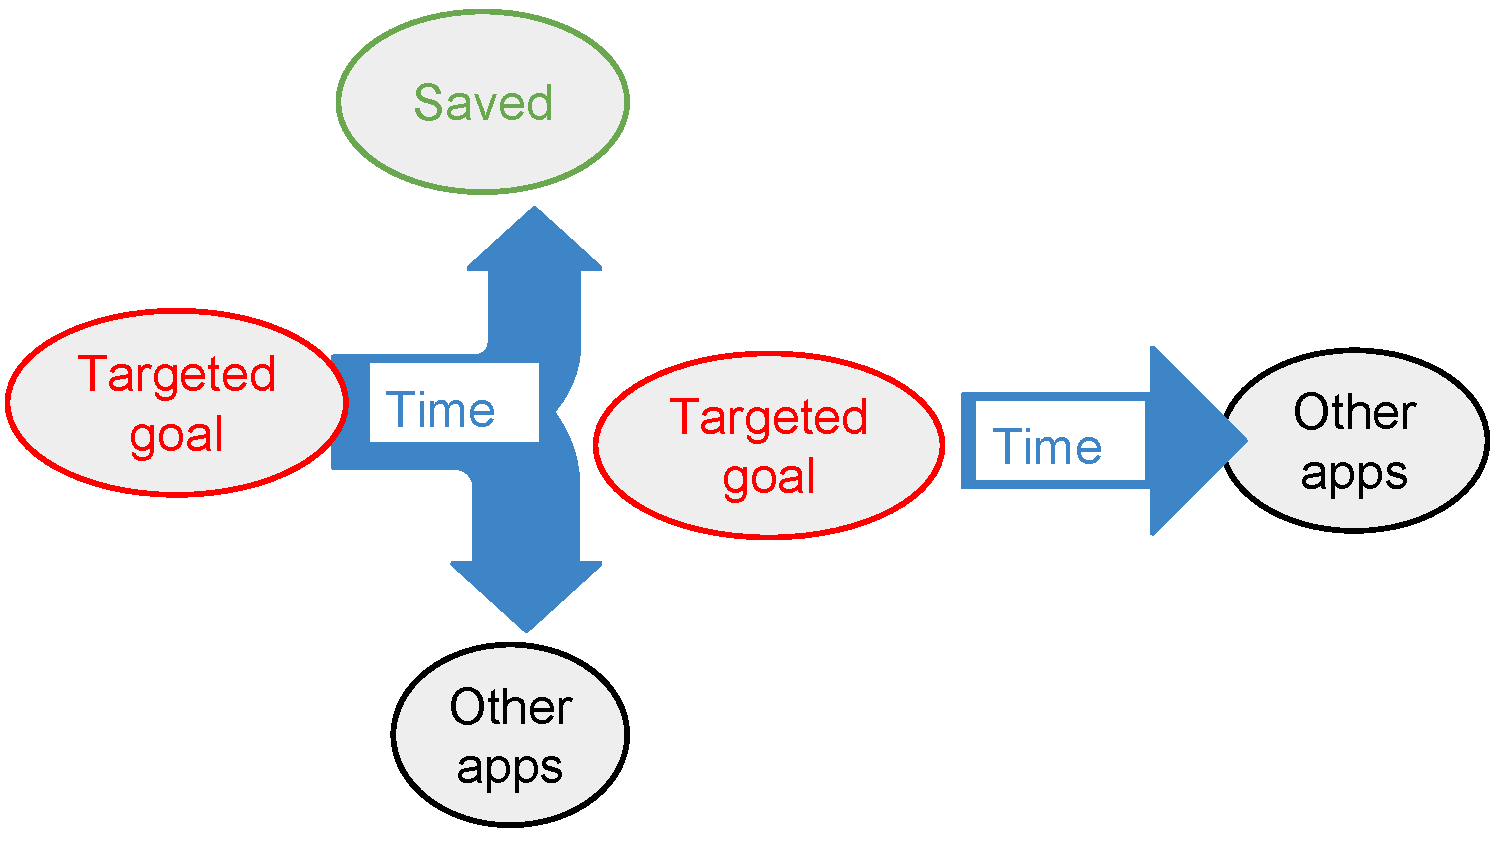
\includegraphics[width=\linewidth]{figures/intro/p01.pdf}
% \caption{}
%   \label{}
% \hfill

% \end{figure}
% \begin{figure}
% 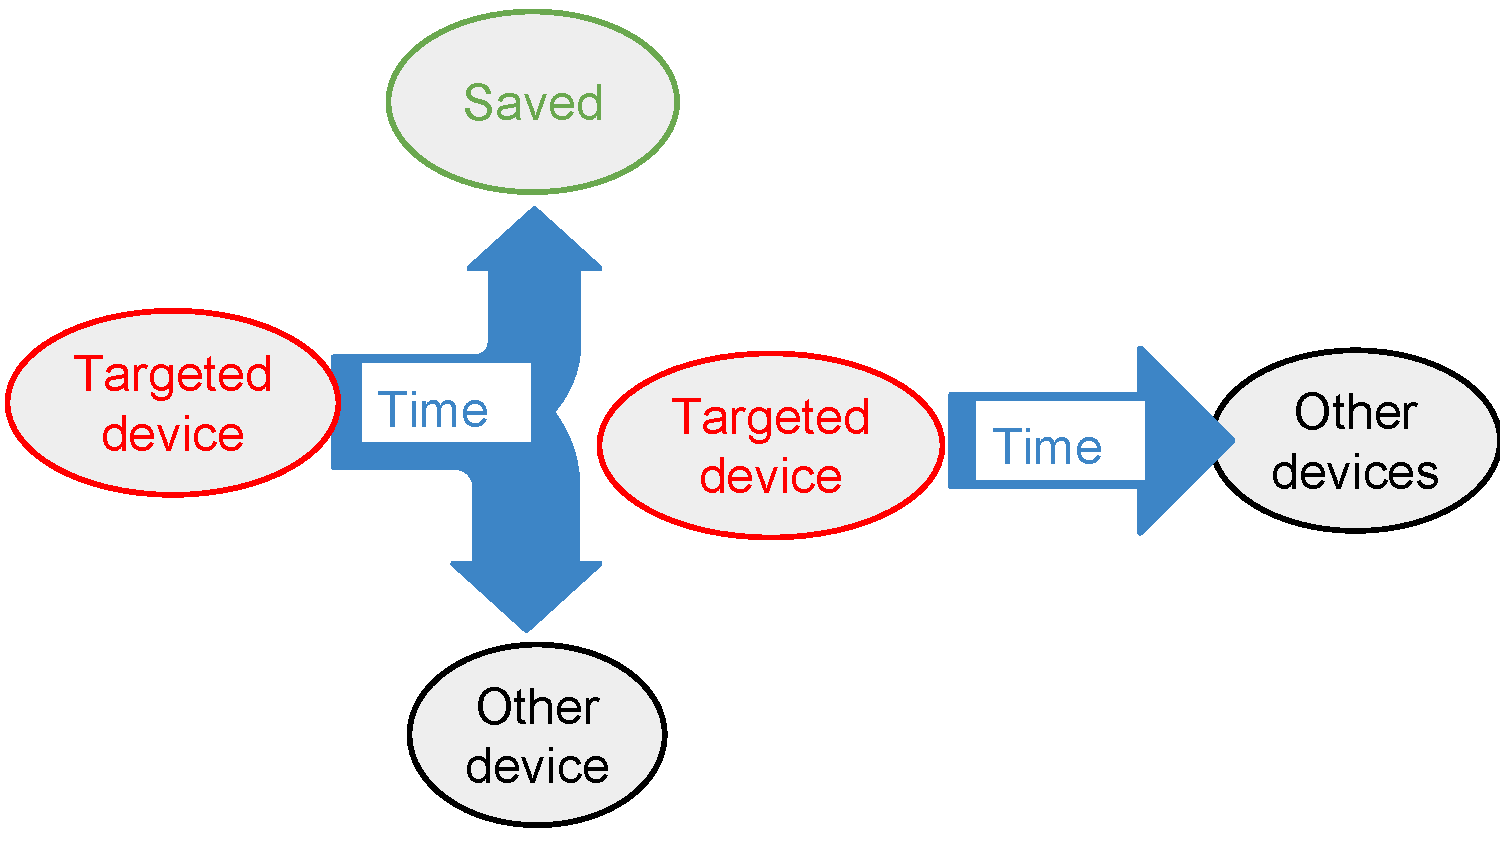
\includegraphics[width=\linewidth]{figures2/intro/p02.pdf}
% \caption{}
%   \label{}
% \hfill

% \end{figure}

% \begin{figure}
% 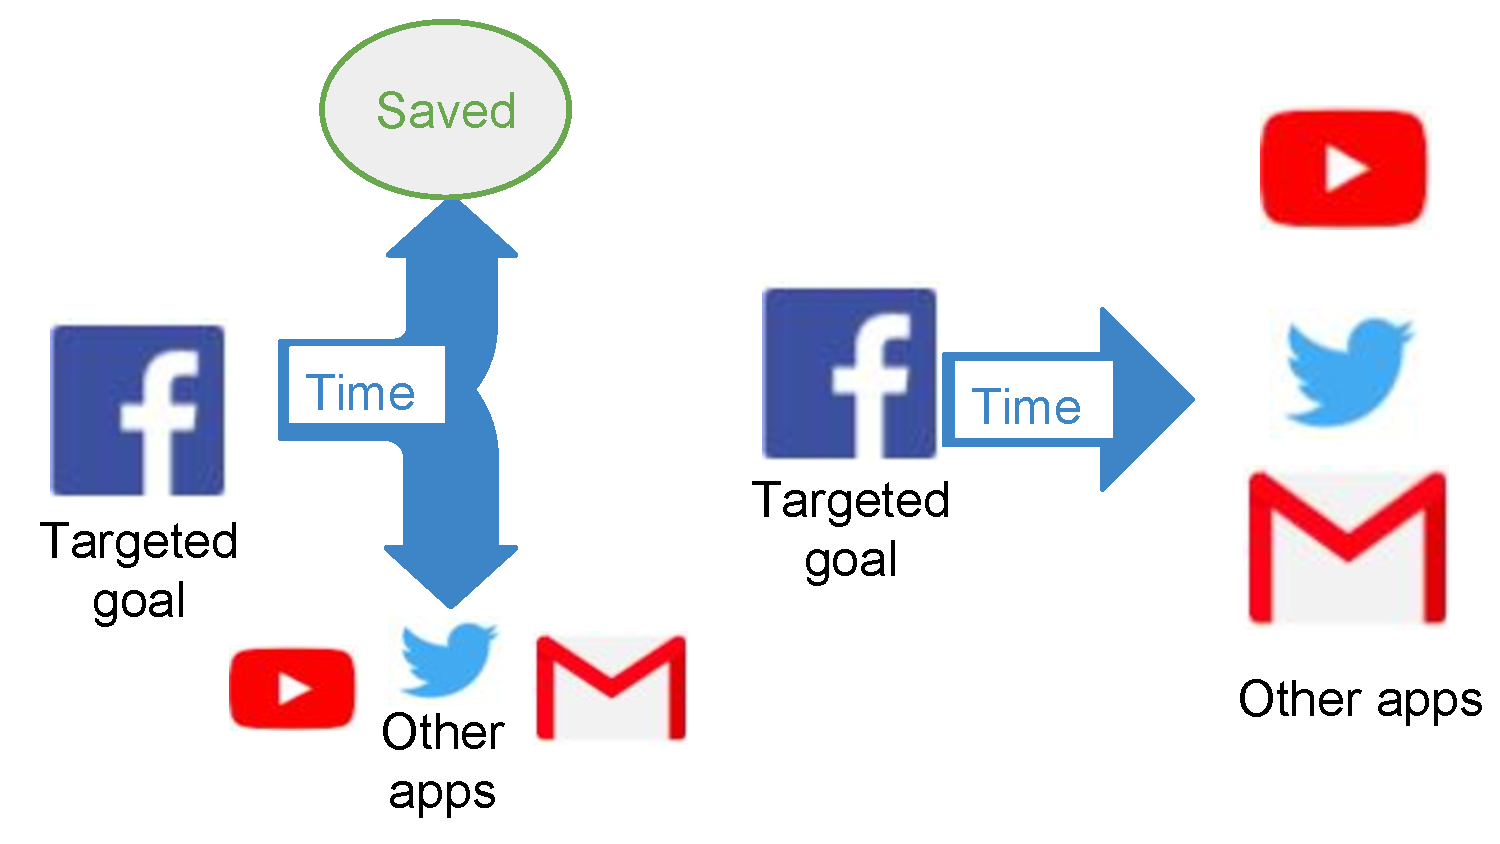
\includegraphics[width=\linewidth]{figures2/intro/p03.pdf}
% \caption{}
%   \label{}  
% \hfill

% \end{figure}
% \begin{figure}
% 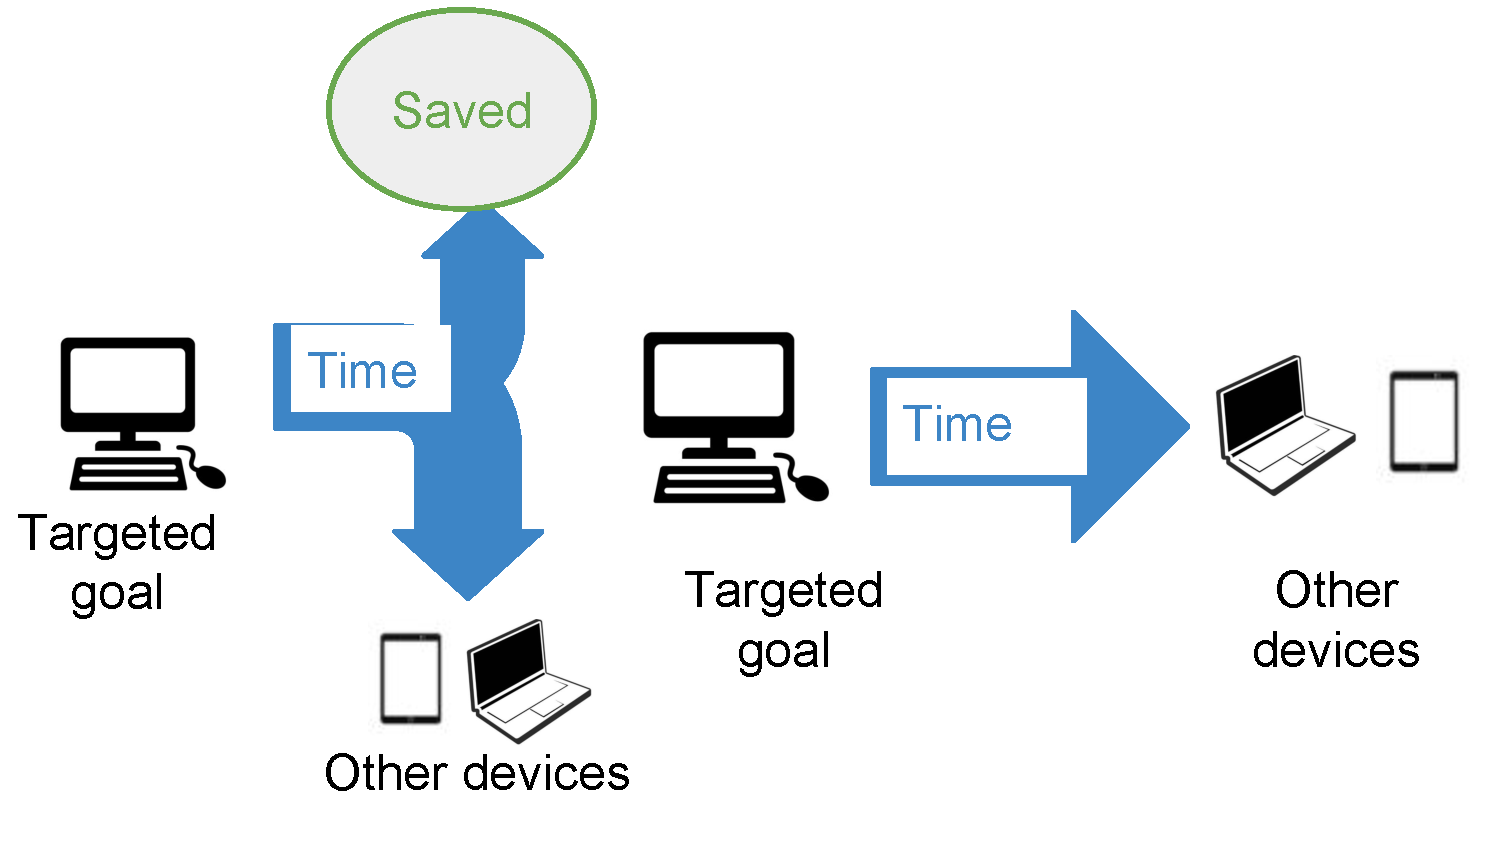
\includegraphics[width=\linewidth]{figures2/intro/p04.pdf}
% \caption{}
%   \label{}
% \hfill

% \end{figure}

\begin{figure}[tb]

%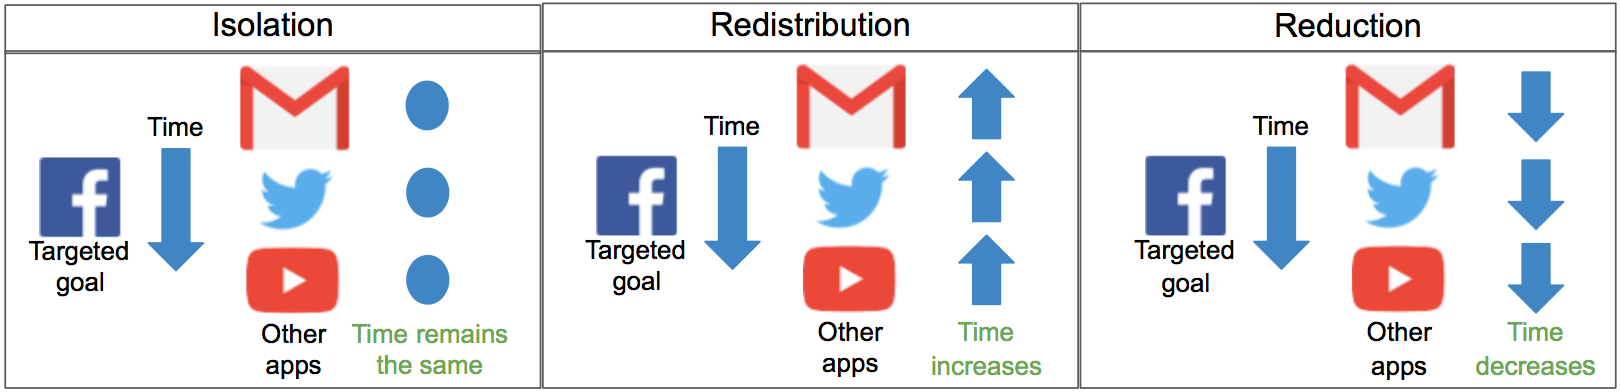
\includegraphics[width=\linewidth, clip,trim=0 0 0.1 0]{figures2/intro/f_1.png}
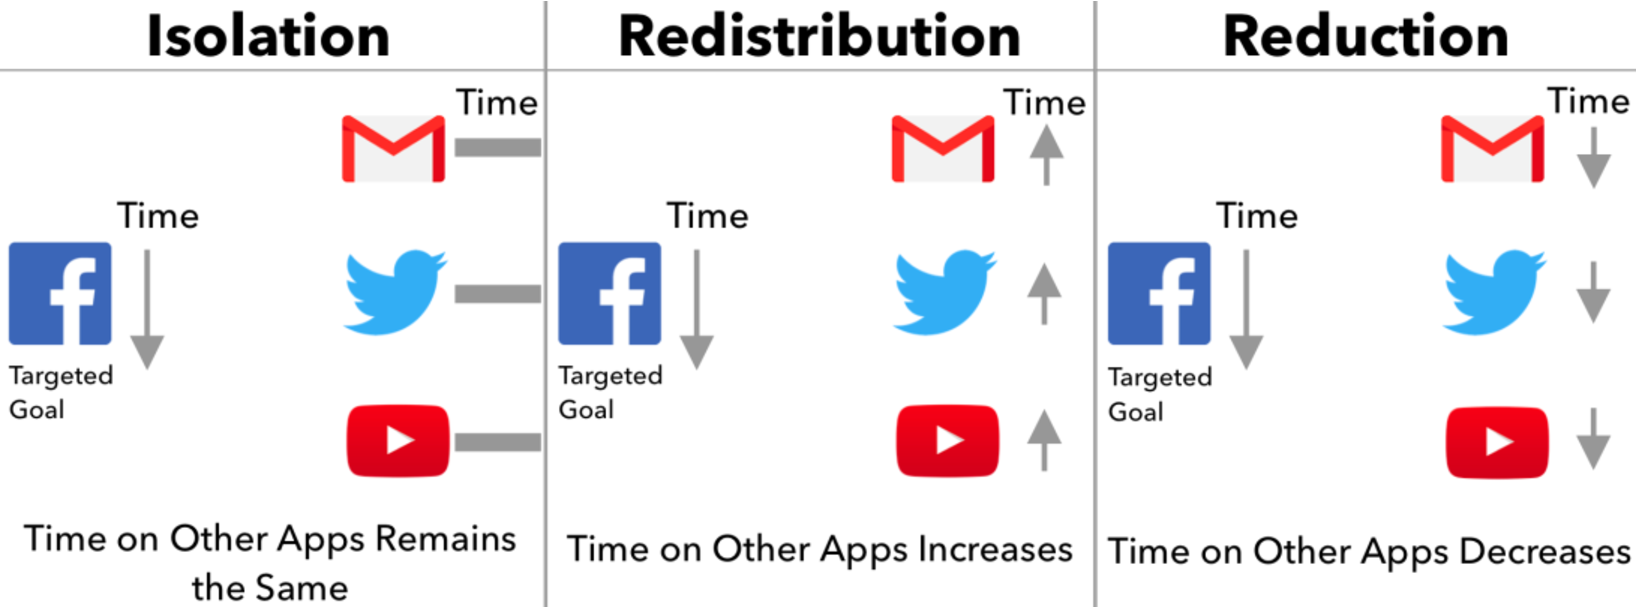
\includegraphics[width=\linewidth, clip,trim=0 0 0.1 0]{figures2/intro/fig1v4.pdf}
\caption{When interventions reduce time on a targeted goal such as Facebook, the time saved may (left)~be isolated from effects on other goals, (center)~be redistributed to other goals, or (right)~decrease time spent on other goals.
%\msb{arrows are too thin, hard to see. fatten 'em up}
%\msb{text is too small to read. don't let it get smaller than the body text of the paper.}
} %\msb{This figure needs to be cleaned up. I see three major goals: first, gestalt grouping and whitespace---things should be close together iff there is meaning in the grouping. For example, arrows should be near the apps that are being affected. Second, use the grid. Right now things are misaligned in many places, like "other apps" vs. "time remains the same". Third, "circle" doesn't convey "no effect" to me. I suggest maybe a dash or flat line? } %\newline
%\goli{Goli: updated figure 1 don't know if it's better or worse}}
%\drew{Drew: I also made a figure (intro/Fig1.pdf) with more space. See which of the three you prefer}

  \label{fig:hypotheses-within}
\end{figure}

\begin{figure}[tb]

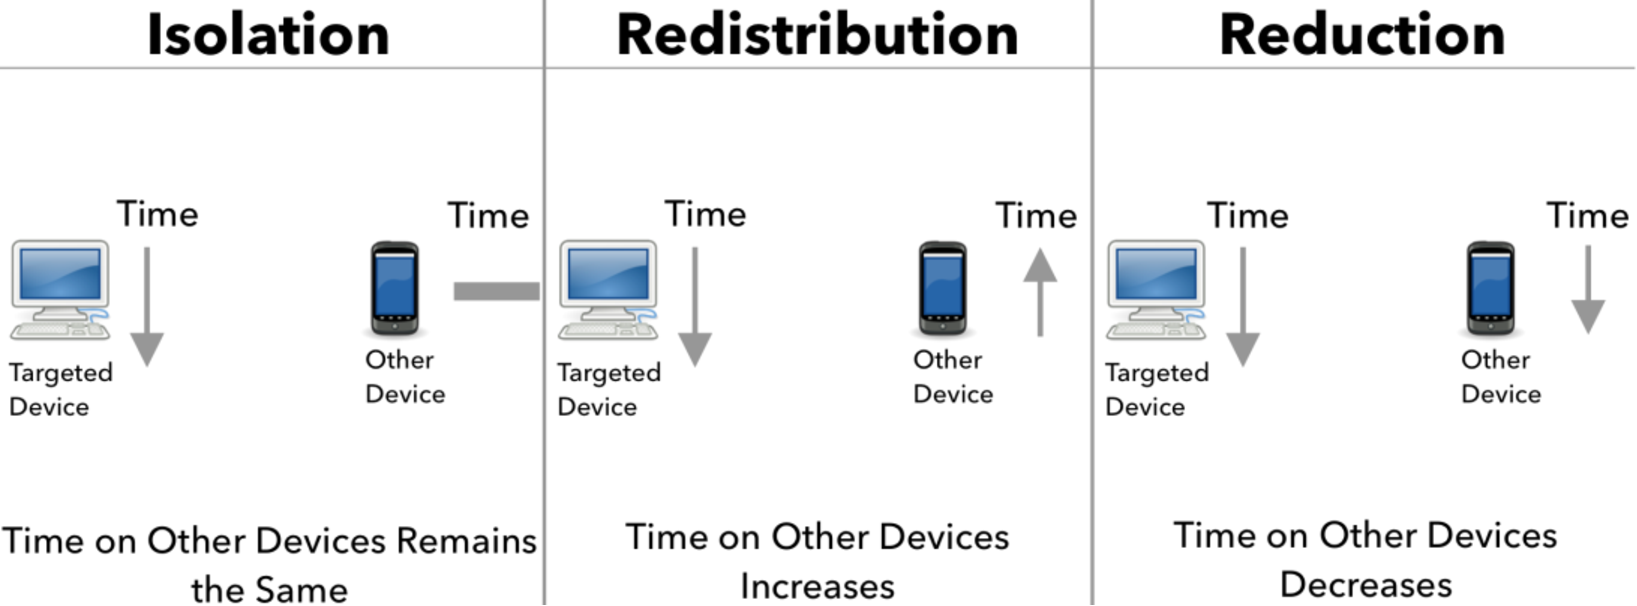
\includegraphics[width=\linewidth]{figures2/intro/fig2v5.pdf}
\caption{When interventions reduce time on a targeted device e.g. a browser, the time saved may (left) be isolated from effects on other devices, (center) be redistributed to other devices, or (right) decrease time spent on other devices.} %platforms similarly to Figure~\ref{fig:hypotheses-within}.
%\msb{arrows are too thin, hard to see. fatten 'em up}
%\msb{text is too small to read. don't let it get smaller than the body text of the paper.}
%}
  \label{fig:hypotheses-across}
\end{figure}

We use productivity behavior change interventions to try to keep ourselves in focus. But do these systems truly save us time? Or do they just redistribute the time elsewhere? In other behavior change domains, interventions sometimes have effects on behaviors other than the ones they were targeting~\cite{stamford1986effects, COTTER2014243}. %There are arguments we can make for several different options.

One possibility is that interventions narrowly impact just the goal that they target, and have no effect on time spent elsewhere. We will refer to this as the \textit{isolated effects hypothesis}. Taking the relationship between time spent on Facebook and Instagram as an example, the isolated effects hypothesis would predict that an intervention that helps reduce time on Facebook should have no effect on time spent on Instagram. Persuasive systems often claim to result in the intended behavioral changes without observable consequences elsewhere, lending support for this hypothesis~\cite{doi:10.1080/15228830802094429,cugelman2013gamification, lyons2014behavior,anderson2013steering, anderson2014engaging}. If the isolated effects hypothesis is true, overall productivity can be boosted through interventions that individually target each goal. %\msb{This paragraph needs grounding through citations in other literature suggesting that it might be the case. Otherwise it's just us handwaving. For example, do we know that smoking cessation interventions don't cause eating problems? The next two paragraphs have a few citations to bolster their case---better examples} %There have been many studies showing that various productivity techniques are effective, so we would hope that overall productivity can be boosted.

However, people have a limited supply of willpower~\cite{baumeister1998ego}, can maintain focus for only so long~\cite{jin2009self,dabbish2011keep,mark2016email}, and need downtime --- so perhaps the time saved is actually just redistributed to other unproductive applications. We will refer to this as the \textit{redistribution hypothesis}: saving time on one unproductive application results in an increase in time spent on other unproductive applications. Returning to our example of a productivity intervention targeting Facebook, redistribution would hypothesize that an intervention that reduces time on Facebook will increase time spent on Instagram.
Redistribution may be partial, where the time redistributed is some fraction of what was saved. Or more bleakly, redistribution may be total, where the time redistributed is entirely shifted to other applications and there is no overall improvement in productivity.
%Within this, there is the possibility for \textit{partial redistribution}, where the amount of time saved in the app/site targeted by the productivity intervention exceeds the amount that is redistributed to other unproductive apps/sites, so overall productivity is still improved, but not as much as we would expect by measuring the effect on the app/site in isolation. A bleaker possibility is \textit{total redistribution}, where amount of time redistributed to other apps equals the time saved on the app targeted by the productivity intervention, so there is overall no improvement in productivity.

A third possibility is that saving time on one application breaks a habit loop~\cite{duhigg2012power} and reduces time spent on other applications as well, so the actual net improvement in productivity is even better than just what is saved on the target application. We will refer to this as the \textit{reduction hypothesis}. Returning to our example of a productivity intervention targeting Facebook, this would hypothesize that an intervention that reduces time on Facebook will also reduce time on Instagram. Perhaps once we enter ``procrastination mode'' and visit one unproductive application, we wind up chaining together visits to another unproductive application, and another---but if a productivity intervention helps us break the chain early on, we will never visit the later unproductive applications.

% Another possibility is a combination of both effects, where overall time is saved but some time is still redistributed to other sources. A third possibility is a symbiotic effect, where 

These three hypotheses lay out the three possibilities of what happens to other goals when we intervene on a focal goal (Figures~\ref{fig:hypotheses-within}--\ref{fig:hypotheses-across}): time on those other goals might stay the same (isolated effects), go up (redistribution), or go down (reduction). In this paper, we seek to adjudicate between these hypotheses using  HabitLab~\cite{habitlab}, an in-the-wild productivity experimentation environment that users can voluntarily participate in by installing. Prior work described HabitLab as a Chrome browser extension; in this paper we created and deployed a companion HabitLab Android application, allowing us to study any redistribution of time that might be happening across devices, as when a user avoids Facebook on their browser but ends up checking Facebook on their phone instead.

After installing and agreeing to our experimental protocol, users specify what they wish to reduce time on, which we term \emph{goals}. In the case of the Android version, goals take the form of applications (apps), whereas on the Chrome extension goals are sites.
We then deploy interventions to help users reduce their time on these goals, which can appear when the user visits a website (Chrome) or app (Android). To study redistribution, we periodically manipulate  the frequency at which interventions appear for each goal --- if the goal is in the frequent condition that week, it will appear every time the user visits that application, whereas if the goal is in the infrequent condition that week, it will appear on 20\% of visits. This experimental design allows us to observe the effects of a goal being in the \textit{frequent} setting not only on how much time users spend on that focal goal, but also what happens to time on other goals when that focal goal is in the frequent setting.

% frequency browser 313 -> 288; mobile 375 -> 235; intensity:browser 978 -> 861; android 3450 -> 3075; within platform browser 3667 -> 3096

Our analysis first begins by seeing whether interventions are effective at reducing time on the focal goal, disregarding any possible redistribution effects. We do so by comparing time spent per day on the application on weeks where interventions are shown frequently, vs those weeks where interventions are shown infrequently. We find that they are effective, with time spent on goal sites reduced by 8.0\% on the Chrome version, and time spent on goal apps reduced by 37.3\% on the Android version.

Next, we investigate whether time is redistributed to other sites/apps on the same platform (browser or mobile) when interventions are frequently shown. We find that giving interventions within the browser produces a reduction effect, with users using sites/apps less when there are more interventions shown on other sites/apps -- however, effects of interventions are isolated on mobile. %\msb{out of date? isolation on one platform, reduction on the other}

Finally, we investigate whether time is redistributed across devices. We do not observe any significant time redistribution effects in either direction.

%Finally, we investigate whether time is redistributed across devices. We find that there is an insignificant trend suggesting an increase in time spent on the browser when a user is given interventions more frequently on Android. \msb{is this up to date?}

This paper contributes a look into potential unintended side effects of productivity interventions on other sites, apps, and devices. We find that productivity interventions do not appear to have deleterious second-order effects on goals other than the ones they are targeting, and in some cases, may even have beneficial second-order effects by breaking habit loops.
%can sometimes have beneficial effects outside the goals they were targeting. %finding that while in some instances there appears to be redistribution, thankfully, it is not a zero-sum game, and there is evidence for global reduction effects.



%----------------------------
% RQ
%----------------------------
% RQ
%\section{Behavior Change and Motivation}

%\msb{Take a pass through this section and remove phrases like "Studies show X" or "Researchers have found X". It's weak writing. Instead just state the claim X. Like instead of "Researchers have found that hotdogs are tasty [cite].", just write "Hotdogs are tasty [cite]." I removed several already.}

% The field of persuasive technology studies how technology can be used to influence behavior~\cite{fogg2002persuasive}. Persuasive technology systems have been successful in promoting behaviors such as sustainable resource usage~\cite{froehlich2009ubigreen}, fitness~\cite{consolvo2008activity}, sleep~\cite{kay2012lullaby,choe2011opportunities}, healthy eating~\cite{noronha2011platemate,epstein2016crumbs}, stress management~\cite{adams2014towards,sanches2010mind}, smoking cessation~\cite{paay2015personal}, and productivity~\cite{whittaker2016don, kim2016timeaware}. An influential framework of behavior change is the B=MAT model~\cite{fogg2002persuasive}, which states that desired behaviors result when motivation, ability, and a trigger (a call to action) are all present. Another framework of habit change is the habit loop~\cite{eyal2014hooked}, which tells us that designs can build habits via a repeated process of displaying a trigger, having the user take an action, providing a reward, and having the user invest in the system.

%\msb{what is lifestyle? it looks like sleep? is this capturing something else? I don't think lifestyle is the right word here}


%\msb{subsection titles for single paragraphs are unnecessary in related work; I'm cutting them}

\section{Related Work}

% Persuasive technologies on computers and mobile phones can help support behavior change. Researchers have developed web-based systems to promote a variety of behavior change goals, including psycho-therapeutic interventions~\cite{doi:10.1080/15228830802094429}, promoting healthy habits~\cite{cugelman2013gamification, lyons2014behavior} and improving educational engagement~\cite{anderson2013steering, anderson2014engaging}. In parallel, a number of studies focus on mobile-based interventions~\cite{paredes2014poptherapy, doi:10.1111/j.1740-9713.2015.00863.x, RILEY201567, anderson2014engaging, FJELDSOE2009165, Whittaker09}. For example, PopTherapy studied micro-interventions for coping with stress using mobile devices~\cite{paredes2014poptherapy}. Likewise, HeartSteps developed an application on mobile phones to promote promote physical activities for individuals~\cite{doi:10.1111/j.1740-9713.2015.00863.x}. % For HabitLab, we developed a version for computers as well as a version for mobile phones. Our study studies user behaviors by evaluating real-time data from both platforms.

% These persuasive technologies have produced measurable beneficial effects. Web-based systems promote a behavior change goals including classroom engagement~\cite{anderson2014engaging, anderson2013steering}, psychology therapy~\cite{doi:10.1080/15228830802094429} and heathy habits~\cite{cugelman2013gamification, lyons2014behavior}. In parallel, a number of studies focused on mobile-based interventions~\cite{paredes2014poptherapy, RILEY201567, FJELDSOE2009165, Whittaker09, info:doi/10.2196/mhealth.4160}. \msb{I don't understand how this paragraph is different from the prior one. Didn't the prior one just list a bunch of domains for behavior change systems?} For instance, MyBehavior, an app on mobile phone, was built to track physical activities of the users and to provide personalized suggestions that are tailored to the users historical behavioral data~\cite{info:doi/10.2196/mhealth.4160}. Similarly, PopTherapy is an a mobile phone application that studied micro-interventions for coping with stress~\cite{paredes2014poptherapy}.

% Measuring the effectiveness of a persuasive system remains a major challenge in behavior change systems design. While behavior change systems can be effective during the experiments~\cite{doi:10.1080/15228830802094429, Cuijpers2008, info:doi/10.2196/jmir.1376}, many review papers are more restrained in whether behavior change systems remain effective outside the studies~\cite{doi:10.1111/j.1467-789X.2009.00646.x, 10.1371/journal.pmed.1000387, NORMAN2007336, 10.1007/978-3-319-07127-5_11}. The critique holds that behavior changes are long, complex processes, and the effectiveness of a system is hard to measure in a short period of time~\cite{prochaska1997transtheoretical}. For instance, an intervention promoting healthy habits, which is effective in changing participants eating habits, might reduce their physical activities which are not measured in the experiment~\cite{COTTER2014243}. Likewise, a system promoting physical activities might have no knowledge on participants' eating habits~\cite{doi:10.1111/j.1740-9713.2015.00863.x}. With interventions on both the computer and the mobile device for each user, our study draws on lived informatics by evaluating the efficacy of productivity interventions in the context of a more complete ecosystem which includes both computers and mobile devices.

Measuring the effectiveness of a persuasive system remains a major challenge in the design of behavior change systems. While behavior change systems can be effective during experiments~\cite{doi:10.1080/15228830802094429, Cuijpers2008, info:doi/10.2196/jmir.1376}, many review papers are more restrained in whether behavior change systems remain effective outside studies and bring longitudinal behavioral change~\cite{doi:10.1111/j.1467-789X.2009.00646.x, 10.1371/journal.pmed.1000387, NORMAN2007336, 10.1007/978-3-319-07127-5_11}. Because behavior changes are long and complex processes, the efficacy of a persuasive system is often difficult to measure~\cite{prochaska1997transtheoretical}. For instance, an intervention promoting healthy habits, which was effective in changing participants' eating habits, might reduce their physical activities, which were not measured in the experiment~\cite{COTTER2014243}. Likewise, a system promoting increased physical activity may be unable to observe effects on participants' eating habits~\cite{doi:10.1111/j.1740-9713.2015.00863.x}. Compared to prior work, our study examines these spillover effects in the context of a more complete ecosystem, including both desktop browsers and mobile devices. % \msb{I don't know what this means}.  \msb{use this paper in the intro to motivate the redistribution hypothesis}

% \msb{This doesn't seem like it's really about multi-device usage} \geza{done}
\subsection{Multitasking and Cyberslacking}
Cyberslacking, referred to as non-work-related computing, is the use of Internet and mobile technology during work hours for personal purposes~\cite{VITAK20111751,PEE2008120, Pamela2004, lim2002}. One study found that employees spent at least one hour on non-work-related activities during a regular work day~\cite{VITAK20111751}. Researchers also reported that non-work-related Internet usage comprises approximately 30\%--50\% of total usage~\cite{RESTUBOG2011247,JAMALUDDIN2015495}. %  \msb{this sentence seems disconnected from everything that came before. why is it here?}.

%\subsection{The Vicious Cycle of Procrastination}

Unproductive time begets further unproductive time. For example, increased time spent online can increase sleep debt, which in turn leads to more time spent online \cite{Mark:2016:SDS:2858036.2858437}. Likewise, the Hook Model claims that many of the most addictive online sites use a cycle of investment techniques to keep users coming back---for example, making a post on Facebook may result in future notifications, which will in turn will get the user to come back and make more posts~\cite{eyal2014hooked}. Finally, sites such as Facebook, Reddit, Twitter, and Buzzfeed are filled with links to each others' content, so it may be the case that increasing usage of one will increase usage of others. If productivity interventions are able to break this vicious cycle of procrastination for one application, they may actually reduce time spent on other unproductive applications as well.

% The importance of understanding the effectiveness of productivity interventions in a complete ecosystem and the rising awareness of unproductive time spent on mobile devices call into focus: would productivity interventions reduce net unproductive time? Or is it a weak palliative with little discernible effect? This led to our research question:

%\begin{resques}[RQ]
%Do productivity interventions reduce net unproductive time, or just redistribute it to other applications, sites, and devices?
%Does rotating interventions is helpful in increasing effectiveness and lowering attrition in online behavior changes systems?}
%\end{resques}

\subsection{Distribution Of Unproductive Time}

%\msb{this is a subsection of measurement, but doesn't seem related?} \geza{done}

%\msb{Same, remove "Studies show X" or "Researchers have found X". } \goli{done}

In this section, we will examine related studies in behavior change systems to develop testable hypotheses regarding the research question. %\msb{what research question? if this is specific to a chapter rather than to the overall contributions, it should be in the relevant chapter} \geza{done}

%\subsection{Intra-device}

Multitasking has become ubiquitous in today's workplaces~\cite{Appelbaum2016, mark2015multitasking, CARRIER2009483}. Multitasking is both essential and unavoidable in the workplace~\cite{freedman2007, mark2008cost}, and it takes 11 minutes on average before people switch to a new task~\cite{dabbish2011keep}. 
% The nature of multitasking in the workspace presents a challenge for designing effective productivity interventions in the face of multiple tasks. %concurrent tasks.
%Researchers also reported multi-tasking on computers is a required skill in employment recruiting nowadays. The study pointed out that an internet-based search of the terms "job description" and "multitasking", by using Google, had over 1.2 million results~\cite{Appelbaum2016}. 
% However, the nature of multitasking in the workspace increases the difficulty of designing effective productivity interventions when there are multiple concurrent tasks. % When one goal increases productivity via an intervention, people might redistribute their unproductive time to other goals instead. \msb{this claim is just thrown out without citations and dropped. either back it up or remove it}
% \msb{inconsistent throughout: is it multitasking or multi-tasking?}

% Persuasive systems often bring the intended behavioral changes (e.g.~\cite{doi:10.1080/15228830802094429,cugelman2013gamification, lyons2014behavior,anderson2013steering, anderson2014engaging}). These results suggest that, at the very least, HabitLab can reduce the time spent on unproductive activities. \msb{I don't see why this paragraph is relevant at all to developing H1 or H2. cut?}

% However, the time spent on unproductive activities might be redistributed elsewhere. While scholars found that persuasive technologies could produce positive outcomes, others worried that interventions could result in negative consequences which might promote users to adopt the opposite target behavior~\cite{10.1007/978-3-319-07127-5_11, 10.1007/978-3-319-31510-2_6}. For example, the tobacco industry sponsored anti-smoking campaign that supports parents to educate their children on risks of smoking could backfire, promoting some teens to light up~\cite{trove.nla.gov.au/work/31391712}. Similarly, researchers who study anti-bullying wristbands found that the wristband campaign increased the chances of bullying for the kids who wear it~\cite{antibullying}. \msb{No, these literatures don't suggest a redistribution hypothesis, it supports a sort of ``reverse effect'' hypothesis where the time on the targeted goal is increased rather than decreased}  This prompts our first hypothesis:
Studying behavior change effects across multiple devices is important: focusing on a single platform will myopically miss unproductive behaviors on other platforms. %because people distributed their unproductive behaviors across multiple People spend time on unproductive activities with computers and mobile phones. 
Attention is fragmented in both mobile and traditional desktop environments~\cite{socialmedia2010, mark2015multitasking}. The time spent on mobile devices has increased more rapidly than time on computers or TVs~\cite{multidevice, nielsen}. On the other hand, mobile applications have been regarded as substitutions of websites in many studies~\cite{10.1007/978-3-642-36516-4_7}. Large technology companies such as Facebook and Amazon have been focusing on user growth on mobile devices~\cite{socialmedia2010}.

However, interventions may result in unintended outcomes~\cite{trove.nla.gov.au/work/31391712, 10.1007/978-3-319-07127-5_11, 10.1007/978-3-319-31510-2_6}. Specifically, while some interventions may be highly effective at achieving the measured goal of a behavioral change system, they may reduce desired outcomes elsewhere~\cite{10.1007/978-3-319-07127-5_11}. In one health-related intervention, while the physical activity of participants increased, calorie intake also increased, working against the goal of promoting a healthy lifestyle~\cite{Blair1985}. Similarly, using peer pressure to build confidence for students at school would, in turn, lower their self-esteem which actually was opposite to the goal of augmenting confidence~\cite{10.1007/978-3-319-31510-2_6}.


\section{Research Questions}

%\msb{Take a pass through this section and remove phrases like "Studies show X" or "Researchers have found X". It's weak writing. Instead just state the claim X. Like instead of "Researchers have found that hotdogs are tasty [cite].", just write "Hotdogs are tasty [cite]." I removed several already.}

% The field of persuasive technology studies how technology can be used to influence behavior~\cite{fogg2002persuasive}. Persuasive technology systems have been successful in promoting behaviors such as sustainable resource usage~\cite{froehlich2009ubigreen}, fitness~\cite{consolvo2008activity}, sleep~\cite{kay2012lullaby,choe2011opportunities}, healthy eating~\cite{noronha2011platemate,epstein2016crumbs}, stress management~\cite{adams2014towards,sanches2010mind}, smoking cessation~\cite{paay2015personal}, and productivity~\cite{whittaker2016don, kim2016timeaware}. An influential framework of behavior change is the B=MAT model~\cite{fogg2002persuasive}, which states that desired behaviors result when motivation, ability, and a trigger (a call to action) are all present. Another framework of habit change is the habit loop~\cite{eyal2014hooked}, which tells us that designs can build habits via a repeated process of displaying a trigger, having the user take an action, providing a reward, and having the user invest in the system.

%\msb{what is lifestyle? it looks like sleep? is this capturing something else? I don't think lifestyle is the right word here}
%Persuasive technologies seek to produce behavioral change~\cite{fogg2002persuasive} across goals as diverse as sustainable resource consumption~\cite{froehlich2009ubigreen}, sleep~\cite{kay2012lullaby,choe2011opportunities}, exercise~\cite{consolvo2008activity}, smoking~\cite{paay2015personal}, eating habits~\cite{noronha2011platemate,epstein2016crumbs}, coping strategies~\cite{adams2014towards,sanches2010mind} and productivity~\cite{whittaker2016don, kim2016timeaware,habitlab}.

%They can operate on many different platforms, such as the web or mobile devices. Web-based systems promote a behavior change goals including classroom engagement~\cite{anderson2014engaging, anderson2013steering}, psychology therapy~\cite{doi:10.1080/15228830802094429} and healthy habits~\cite{cugelman2013gamification, lyons2014behavior}. In parallel, a number of studies focused on mobile-based interventions~\cite{paredes2014poptherapy, RILEY201567, FJELDSOE2009165, Whittaker09, info:doi/10.2196/mhealth.4160}. For instance, MyBehavior, a mobile phone app, was built to track physical activities of the users and to provide personalized suggestions that are tailored to the users' historical behavioral data~\cite{info:doi/10.2196/mhealth.4160}. Similarly, PopTherapy is a mobile phone app that studied micro-interventions for coping with stress~\cite{paredes2014poptherapy}.

%There are a number of theoretical frameworks describing behavior change systems. B=MAT is a popular framework of behavioral change~\cite{fogg2002persuasive}, which demonstrates that systems can focus on three elements---motivation, ability, and a trigger (a call to action)---to produce behavior change. The habit loop is another framework for building habits~\cite{eyal2014hooked}, stating that systems can build habits through an iterated process of displaying a trigger, prompting the user to take an action, giving out a reward, and helping the user to invest in the system.

%\msb{subsection titles for single paragraphs are unnecessary in related work; I'm cutting them}

%\subsection{Effectiveness Measurements}

% Persuasive technologies on computers and mobile phones can help support behavior change. Researchers have developed web-based systems to promote a variety of behavior change goals, including psycho-therapeutic interventions~\cite{doi:10.1080/15228830802094429}, promoting healthy habits~\cite{cugelman2013gamification, lyons2014behavior} and improving educational engagement~\cite{anderson2013steering, anderson2014engaging}. In parallel, a number of studies focus on mobile-based interventions~\cite{paredes2014poptherapy, doi:10.1111/j.1740-9713.2015.00863.x, RILEY201567, anderson2014engaging, FJELDSOE2009165, Whittaker09}. For example, PopTherapy studied micro-interventions for coping with stress using mobile devices~\cite{paredes2014poptherapy}. Likewise, HeartSteps developed an application on mobile phones to promote promote physical activities for individuals~\cite{doi:10.1111/j.1740-9713.2015.00863.x}. % For HabitLab, we developed a version for computers as well as a version for mobile phones. Our study studies user behaviors by evaluating real-time data from both platforms.

% These persuasive technologies have produced measurable beneficial effects. Web-based systems promote a behavior change goals including classroom engagement~\cite{anderson2014engaging, anderson2013steering}, psychology therapy~\cite{doi:10.1080/15228830802094429} and heathy habits~\cite{cugelman2013gamification, lyons2014behavior}. In parallel, a number of studies focused on mobile-based interventions~\cite{paredes2014poptherapy, RILEY201567, FJELDSOE2009165, Whittaker09, info:doi/10.2196/mhealth.4160}. \msb{I don't understand how this paragraph is different from the prior one. Didn't the prior one just list a bunch of domains for behavior change systems?} For instance, MyBehavior, an app on mobile phone, was built to track physical activities of the users and to provide personalized suggestions that are tailored to the users historical behavioral data~\cite{info:doi/10.2196/mhealth.4160}. Similarly, PopTherapy is an a mobile phone application that studied micro-interventions for coping with stress~\cite{paredes2014poptherapy}.

% Measuring the effectiveness of a persuasive system remains a major challenge in behavior change systems design. While behavior change systems can be effective during the experiments~\cite{doi:10.1080/15228830802094429, Cuijpers2008, info:doi/10.2196/jmir.1376}, many review papers are more restrained in whether behavior change systems remain effective outside the studies~\cite{doi:10.1111/j.1467-789X.2009.00646.x, 10.1371/journal.pmed.1000387, NORMAN2007336, 10.1007/978-3-319-07127-5_11}. The critique holds that behavior changes are long, complex processes, and the effectiveness of a system is hard to measure in a short period of time~\cite{prochaska1997transtheoretical}. For instance, an intervention promoting healthy habits, which is effective in changing participants eating habits, might reduce their physical activities which are not measured in the experiment~\cite{COTTER2014243}. Likewise, a system promoting physical activities might have no knowledge on participants' eating habits~\cite{doi:10.1111/j.1740-9713.2015.00863.x}. With interventions on both the computer and the mobile device for each user, our study draws on lived informatics by evaluating the efficacy of productivity interventions in the context of a more complete ecosystem which includes both computers and mobile devices.

%Measuring the effectiveness of a persuasive system remains a major challenge in the design of behavior change systems. While behavior change systems can be effective during experiments~\cite{doi:10.1080/15228830802094429, Cuijpers2008, info:doi/10.2196/jmir.1376}, many review papers are more restrained in whether behavior change systems remain effective outside studies and bring longitudinal behavioral change~\cite{doi:10.1111/j.1467-789X.2009.00646.x, 10.1371/journal.pmed.1000387, NORMAN2007336, 10.1007/978-3-319-07127-5_11}. Because behavior changes are long and complex processes, the efficacy of a persuasive system is often difficult to measure~\cite{prochaska1997transtheoretical}. For instance, an intervention promoting healthy habits, which was effective in changing participants' eating habits, might reduce their physical activities, which were not measured in the experiment~\cite{COTTER2014243}. Likewise, a system promoting increased physical activity may be unable to observe effects on participants' eating habits~\cite{doi:10.1111/j.1740-9713.2015.00863.x}. Compared to prior work, our study examines these spillover effects in the context of a more complete ecosystem, including both desktop browsers and mobile devices. % \msb{I don't know what this means}.  \msb{use this paper in the intro to motivate the redistribution hypothesis}

%\subsection{Multi-Device Usage}

%Cyberslacking, referred to as non-work-related computing, is the use of Internet and mobile technology during work hours for personal purposes~\cite{VITAK20111751,PEE2008120, Pamela2004, lim2002}. One study found that employees spent at least one hour on non-work-related activities during a regular work day~\cite{VITAK20111751}. Researchers also reported that non-work-related Internet usage comprises approximately 30\%--50\% of total usage~\cite{RESTUBOG2011247,JAMALUDDIN2015495}. %  \msb{this sentence seems disconnected from everything that came before. why is it here?}.

%\subsection{The Vicious Cycle of Procrastination}

Unproductive time begets further unproductive time. For example, increased time spent online can increase sleep debt, which in turn leads to more time spent online \cite{Mark:2016:SDS:2858036.2858437}. Likewise, the Hook Model claims that many of the most addictive online sites use a cycle of investment techniques to keep users coming back---for example, making a post on Facebook may result in future notifications, which will in turn will get the user to come back and make more posts~\cite{eyal2014hooked}. Finally, sites such as Facebook, Reddit, Twitter, and Buzzfeed are filled with links to each others' content, so it may be the case that increasing usage of one will increase usage of others. If productivity interventions are able to break this vicious cycle of procrastination for one application, they may actually reduce time spent on other unproductive applications as well.

The importance of understanding the effectiveness of productivity interventions in a complete ecosystem and the rising awareness of unproductive time spent on mobile devices call into focus: would productivity interventions reduce net unproductive time? Or is it a weak palliative with little discernible effect? This led to our research question:

\begin{resques}[RQ]
Do productivity interventions reduce net unproductive time, or just redistribute it to other applications, sites, and devices?
%Does rotating interventions is helpful in increasing effectiveness and lowering attrition in online behavior changes systems?}
\end{resques}

%\section{Distribution Of Unproductive Time}

%\msb{Same, remove "Studies show X" or "Researchers have found X". } \goli{done}

%In this section, we will examine related studies in behavior change systems to develop testable hypotheses regarding the research question.

%\subsection{Intra-device}

%Multitasking has become ubiquitous in today's workplaces~\cite{Appelbaum2016, mark2015multitasking, CARRIER2009483}. Multitasking is both essential and unavoidable in the workplace~\cite{freedman2007, mark2008cost}, and it takes 11 minutes on average before people switch to a new task~\cite{dabbish2011keep}. 
% The nature of multitasking in the workspace presents a challenge for designing effective productivity interventions in the face of multiple tasks. %concurrent tasks.
%Researchers also reported multi-tasking on computers is a required skill in employment recruiting nowadays. The study pointed out that an internet-based search of the terms "job description" and "multitasking", by using Google, had over 1.2 million results~\cite{Appelbaum2016}. 
% However, the nature of multitasking in the workspace increases the difficulty of designing effective productivity interventions when there are multiple concurrent tasks. % When one goal increases productivity via an intervention, people might redistribute their unproductive time to other goals instead. \msb{this claim is just thrown out without citations and dropped. either back it up or remove it}
% \msb{inconsistent throughout: is it multitasking or multi-tasking?}

% Persuasive systems often bring the intended behavioral changes (e.g.~\cite{doi:10.1080/15228830802094429,cugelman2013gamification, lyons2014behavior,anderson2013steering, anderson2014engaging}). These results suggest that, at the very least, HabitLab can reduce the time spent on unproductive activities. \msb{I don't see why this paragraph is relevant at all to developing H1 or H2. cut?}

% However, the time spent on unproductive activities might be redistributed elsewhere. While scholars found that persuasive technologies could produce positive outcomes, others worried that interventions could result in negative consequences which might promote users to adopt the opposite target behavior~\cite{10.1007/978-3-319-07127-5_11, 10.1007/978-3-319-31510-2_6}. For example, the tobacco industry sponsored anti-smoking campaign that supports parents to educate their children on risks of smoking could backfire, promoting some teens to light up~\cite{trove.nla.gov.au/work/31391712}. Similarly, researchers who study anti-bullying wristbands found that the wristband campaign increased the chances of bullying for the kids who wear it~\cite{antibullying}. \msb{No, these literatures don't suggest a redistribution hypothesis, it supports a sort of ``reverse effect'' hypothesis where the time on the targeted goal is increased rather than decreased}  This prompts our first hypothesis:
Studying behavior change effects across multiple devices is important: focusing on a single platform will myopically miss unproductive behaviors on other platforms. %because people distributed their unproductive behaviors across multiple People spend time on unproductive activities with computers and mobile phones. 
Attention is fragmented in both mobile and traditional desktop environments~\cite{socialmedia2010, mark2015multitasking}. The time spent on mobile devices has increased more rapidly than time on computers or TVs~\cite{multidevice, nielsen}. On the other hand, mobile applications have been regarded as substitutions of websites in many studies~\cite{10.1007/978-3-642-36516-4_7}. Large technology companies such as Facebook and Amazon have been focusing on user growth on mobile devices~\cite{socialmedia2010}.

However, interventions may result in unintended outcomes~\cite{trove.nla.gov.au/work/31391712, 10.1007/978-3-319-07127-5_11, 10.1007/978-3-319-31510-2_6}. Specifically, while some interventions may be highly effective at achieving the measured goal of a behavioral change system, they may reduce desired outcomes elsewhere~\cite{10.1007/978-3-319-07127-5_11}. In one health-related intervention, while the physical activity of participants increased, calorie intake also increased, working against the goal of promoting a healthy lifestyle~\cite{Blair1985}. Similarly, using peer pressure to build confidence for students at school would, in turn, lower their self-esteem which actually was opposite to the goal of augmenting confidence~\cite{10.1007/978-3-319-31510-2_6}.

In our system, the time spent on unproductive activities might be decreased in one application yet increased in others. These prompt our hypotheses:
% \msb{didn't this come up in the previous section? move that down here, don't repeat yourself} \msb{runon sentence:}

\begin{hyp}[H\ref*{hyp:within}] \label{hyp:within}
Within a single device, productivity interventions will cause the time spent on targeted sites and apps to be redistributed to other sites and apps. 
\end{hyp}

%\subsection{Inter-devices}

% Researchers found multi-tasking behaviors across different devices including computers and mobiles~\cite{Appelbaum2016}. Studies demonstrated that employees who spend time on non-work-related computing during working hours on both Internet and mobile technology~\cite{VITAK20111751}. \jake{I don't know what the preceeding sentence is trying to say. does spending time on non-related computing do something, or is this behavior simply observed?} Furthermore, some studies showed that the user growth rate is higher on mobile devices than on computers~\cite{multidevice}. \msb{Again, none of these results directly suggest this hypothesis.} In light of these results, we hypothesize:


%\msb{awkward phrasing:} \goli{changed first sentence!!}
% Mobile devices play an increasingly important role in our daily lives~\cite{multidevice} \msb{didn't you make this point in the previous section?}. Researchers found multitasking behaviors across different devices including mobile devices~\cite{Appelbaum2016}. Especially, people spent a significant portion of working hours on mobiles devices for unproductive activities~\cite{VITAK20111751}. \msb{all of these seem to echo the previous section?} As mobile phones become popular devices for unproductive activities in workspace, our interventions might increase productivity on computer while decrease on mobile devices. Similar to the intra-device's speculation, we hypothesize:

% \msb{that paragraph didn't do anything for me. I might be missing something, but my sense is that none of these papers make any kind of cross-platform redistribution prediction. if you don't have any evidence about cross-platform bleeding, then I would just go directly from H1 to H2, since the same causal pathway would lead to both}

\begin{hyp}[H\ref*{hyp:across}] \label{hyp:across}
Between computers and mobile devices, productivity interventions will cause the time spent on one device to be redistributed to other devices.
\end{hyp}


% % The challenges of static interventions, and the rising wave of personalization systems, call into focus: would a rotation strategy work? Or is it a weak palliative with little discernible effect? This led to our research question:

% \begin{resques}[RQ]
% Can a strategy of rotating interventions produce more effective behavior change systems?
% %Does rotating interventions is helpful in increasing effectiveness and lowering attrition in online behavior changes systems?}
% \end{resques}

% \rev{One major topic inspiring our work is users' desires to curb or control their time spent on social media sites. People pressure themselves to, and often do, make efforts to reduce their time spent on social media sites such as Facebook and Twitter~\cite{Sleeper:2015:ILI:2675133.2675193,schoenebeck2014giving}. Yet this is difficult because users turn to social media to address their need to belong, the need for self-presentation, the need for self-esteem~\cite{nadkarni2012people}, the need for entertainment and gratification ~\cite{raacke2008myspace}, and self-affirmation ~\cite{toma2013self}. Whether social media use improves well-being is a complex question depending on the nature of the engagement ~\cite{uysal2013mediating, marche2012facebook, lin2015emotional, kim2011facebook, muise2009more, sagioglou2014facebook, tandoc2015facebook}, but thanks to instant gratification and sites' use of gamification~\cite{chou2015actionable, zichermann2011gamification, huotari2012defining} and behavior design techniques~\cite{fogg2002persuasive, eyal2014hooked} to drive engagement, users keep coming back, to the point that some consider it an addiction~\cite{andreassen2012development, ryan2014uses, tang2016personality, turel2014examination}.} %Furthermore, social media sites make heavy use of gamification to drive engagement on their sites~\cite{chou2015actionable, zichermann2011gamification, huotari2012defining}, and are cited as successful applications of behavior change theories~\cite{fogg2002persuasive, eyal2014hooked}.} %Furthermore, social media sites are designed to maximize user engagement, with features closely following gamification strategies~\cite{chou2015actionable} and behavior change theories~\cite{fogg2002persuasive, eyal2014hooked}.}


%----------------------------


%----------------------------
% RQ 
% \section{Behavior Change And Motivation}
% The field of persuasive technology studies how technology can be used to influence behavior~\cite{fogg2002persuasive}. Persuasive technology systems have been successful in promoting behaviors such as sustainable resource usage~\cite{froehlich2009ubigreen}, fitness~\cite{consolvo2008activity}, sleep~\cite{kay2012lullaby,choe2011opportunities}, healthy eating~\cite{noronha2011platemate,epstein2016crumbs}, stress management~\cite{adams2014towards,sanches2010mind}, smoking cessation~\cite{paay2015personal}, and productivity~\cite{whittaker2016don, kim2016timeaware}. An influential framework of behavior change is the B=MAT model~\cite{fogg2002persuasive}, which states that desired behaviors result when motivation, ability, and a trigger (a call to action) are all present. Another framework of habit change is the habit loop~\cite{eyal2014hooked}, which tells us that designs can build habits via a repeated process of displaying a trigger, having the user take an action, providing a reward, and having the user invest in the system.

% A number of taxonomies characterize the design space of interventions, both general~\cite{michie2013behavior, behaviourchangewheel, abraham2008taxonomy, dolanmindspace} and domain-specific~\cite{hardeman2000interventions, west2010behavior}. Michie's behavior change taxonomy lists 93 techniques for behavior change, clustered according to the cognitive phenomenon they target~\cite{michie2013behavior}. Systems have investigated effects of these techniques individually, such as using ``cheating'' to support lapse management~\cite{agapie2016staying}, using different framings to present results~\cite{kim2016timeaware}, or setting goals and plans~\cite{agapie2016plansourcing}.

% % One of the most comprehensive investigations we
% % identified is a recent meta-analysis of 85 studies by
% % Webb et al. (2010) that found interventions that were
% % strongly based in theory had greater impact than those
% % that were not, and interventions that incorporated more
% % behavior change techniques tended to have larger
% % effects than interventions that incorporated fewer techniques

% % Within the CSCW community, behavior change has been an active area of research. One major topic inspiring our work is users' desires to curb or control their time spent on social media sites. People pressure themselves to, and often do, make efforts to reduce their time spent on social media sites such as Facebook and Twitter~\cite{Sleeper:2015:ILI:2675133.2675193,schoenebeck2014giving}. This paper builds on this literature, contributing studies of how people might become more effective at this goal. Sociotechnical systems are also locations where people discuss behavior change~\cite{chancellornorms}, and find social support~\cite{Ko:2015:NGI:2675133.2675244, Chung:2017:PTB:3025453.3025747}. Behavior change often requires self-tracking, self-experimentation, and personal informatics~\cite{Karkar:2017:TFS:3025453.3025480}, leading to opportunities to share data and progress with trusted others~\cite{Chung:2016:BNA:2818048.2819926, pina2017personal}.

% \rev{People use a variety of sociotechnical systems to support behavior change, including forums~\cite{eysenbach2004health, chancellornorms}, social sharing~\cite{poirier2012social, Chung:2016:BNA:2818048.2819926, pina2017personal, Ko:2015:NGI:2675133.2675244}, personal informatics~\cite{li2010stage, Chung:2017:PTB:3025453.3025747}, and self-experimentation~\cite{Karkar:2017:TFS:3025453.3025480}. People use behavior change forums to gain social support~\cite{hong2012outcomes} -- meeting social needs such as approval and esteem~\cite{kaplan1977social}. They do so by providing users with information and advice~\cite{hong2012outcomes}, and establishing norms~\cite{chancellornorms}. They also facilitate social comparisons~\cite{davison2000talks} which influence behaviors, as social comparison theory states that users seek to bring their behaviors in line with norms~\cite{festinger1954theory}. Communities also help users find others with similar experiences~\cite{huh2014health} who can help them through the process of recovering and adapting to changes~\cite{newman2011s}. Social sharing~\cite{poirier2012social, richardson2010online} works by helping users receive support through social interactions, and encouraging accountability~\cite{epstein2015nobody}. Personal informatics support behavior change through stages of preparation, collection, integration, reflection, and action~\cite{li2010stage}. The theory of lived informatics~\cite{epstein2015lived} adds additional stages where users choose tracking tools, and alternate between lapsing and resuming their tracking behaviors. HabitLab combines personal informatics and self-experimentation to support behavior change. Our study draws on lived informatics by evaluating whether rotating interventions is an effective strategy to combat lapses such as ignoring interventions or uninstalling.}

% % Of course, sociotechnical systems may also have deleterious effects --- communities may set unhealthy norms such as encouraging eating disorders~\cite{chancellornorms}, and social sharing can cause anxiety~\cite{munson2010happier}, impression management concerns~\cite{consolvo2014designing}, and make users unwilling to set goals~\cite{munson2015effects}.

% % \msb{Can you pull this together into a summary of what we draw from this literature and how it influences HabitLab or our study?}

% \rev{One major topic inspiring our work is users' desires to curb or control their time spent on social media sites. People pressure themselves to, and often do, make efforts to reduce their time spent on social media sites such as Facebook and Twitter~\cite{Sleeper:2015:ILI:2675133.2675193,schoenebeck2014giving}. Yet this is difficult because users turn to social media to address their need to belong, the need for self-presentation, the need for self-esteem~\cite{nadkarni2012people}, the need for entertainment and gratification ~\cite{raacke2008myspace}, and self-affirmation ~\cite{toma2013self}. Whether social media use improves well-being is a complex question depending on the nature of the engagement ~\cite{uysal2013mediating, marche2012facebook, lin2015emotional, kim2011facebook, muise2009more, sagioglou2014facebook, tandoc2015facebook}, but thanks to instant gratification and sites' use of gamification~\cite{chou2015actionable, zichermann2011gamification, huotari2012defining} and behavior design techniques~\cite{fogg2002persuasive, eyal2014hooked} to drive engagement, users keep coming back, to the point that some consider it an addiction~\cite{andreassen2012development, ryan2014uses, tang2016personality, turel2014examination}.} %Furthermore, social media sites make heavy use of gamification to drive engagement on their sites~\cite{chou2015actionable, zichermann2011gamification, huotari2012defining}, and are cited as successful applications of behavior change theories~\cite{fogg2002persuasive, eyal2014hooked}.} %Furthermore, social media sites are designed to maximize user engagement, with features closely following gamification strategies~\cite{chou2015actionable} and behavior change theories~\cite{fogg2002persuasive, eyal2014hooked}.}

% % datu2012does

% % Social media is particularly addictive be

% % \rev{expanded the related work discussion on sociotechnical theories. list the theories driving these papers. social support cscw theories. why people use forums for behavior change support what role do other people play in driving your behavior change. collective exercise. why are social media particularly hard to manage your behavior with why is social media addictive.}

% % \rev{festinger's social comparison theory postulated that social behaviors could be predicted largely on the basis of the assumption that individuals seek to have and maintain a sense of normalcy and accuracy about the world}

% % http://journals.sagepub.com/doi/pdf/10.1177/1524839911405850
% % Harnessing Social Media for Health Promotion and Behavior Change

% % \rev{Communities and collaborative support can help achieve behavior change goals. }

% Much previous work has focused on gamification as an approach to design behavior change systems~\cite{deterding2011game}. Gamification has been shown to have positive effects on engagement and outcomes in behavior-change contexts such as promoting healthy habits~\cite{cugelman2013gamification, lyons2014behavior} and improving  educational engagement~\cite{anderson2013steering, anderson2014engaging}, though effectiveness varies depending on the context and design~\cite{6758978}. % Popular online services such as Facebook and LinkedIn make heavy use of gamification to drive engagement on their sites~\cite{chou2015actionable, zichermann2011gamification, huotari2012defining}.

% Attrition is a major challenge in behavior change systems. Attrition~\cite{eysenbach2005law}, also known as dropout, occurs when participants stop participating, leave, or uninstall the system. Persuasive systems built for weight control and therapy have shown substantial attrition rates in longitudinal studies~\cite{Bernier1986,paredes2014poptherapy}, and prior work in CSCW has sought to help reduce attrition rates through techniques drawn from dieting and addiction research~\cite{agapie2016staying}. % This paper contributes a direct study of attrition and its antecedents.%this study the increments in attrition has not been discussed in detail or quantified in the context of rotating interventions in behavior change systems.

% A recent trend in behavior change systems has been the concept of personalizing interventions. Such systems explore several possible strategies using techniques such as multi-armed bandits to find the intervention that is most effective for the user~\cite{paredes2014poptherapy, rabbi2014automated}. For example, PopTherapy demonstrated personalized messaging could be found through such techniques~\cite{paredes2014poptherapy}. Likewise, HeartSteps conducted tens or hundreds of micro-randomized trials on users~\cite{doi:10.1111/j.1740-9713.2015.00863.x}.  When multi-armed bandits are just beginning to get feedback from a user, they will try out several different interventions to see what works. This exploration has the effect of rotation, but the amount of rotation declines as the bandit begins to personalize. In this paper, we examine the contrarian assertion that perhaps rotation should be maintained to sustain novelty even after the multi-armed bandit is aware of which intervention is most effective for the user.

% % The challenges of static interventions, and the rising wave of personalization systems, call into focus: would a rotation strategy work? Or is it a weak palliative with little discernible effect? This led to our research question:

% \begin{resques}[RQ]
% Can a strategy of rotating interventions produce more effective behavior change systems?
% %Does rotating interventions is helpful in increasing effectiveness and lowering attrition in online behavior changes systems?}
% \end{resques}

%----------------------------
% HYP
%\section{Rotating Interventions}
%In this section, we review literature in behavior change systems and psychology to develop specific testable predictions regarding the research question.% Few studies has touched upon the quantification of effectiveness and attrition in the literature of online behavior changes systems. However, there are studies in behavior changes systems investigating the effectiveness of algorithmic interventions system. Meanwhile, previous work in behavior-change contexts has shown the porblem of attrition of behavioral interventions. This section presents a review of such studies and the proposal of our research hypotheses. 

% \jingyi{reviewed papers? i would just say past work}
%\subsection{Effectiveness over time}
%While behavior change systems can be effective~\cite{doi:10.1080/15228830802094429, Cuijpers2008, info:doi/10.2196/jmir.1376}, many review papers are more restrained in whether behavior change systems remain effective over long periods of time~\cite{doi:10.1111/j.1467-789X.2009.00646.x, 10.1371/journal.pmed.1000387, NORMAN2007336, 10.1007/978-3-319-07127-5_11}. The critique holds that behavior changes are long, complex processes, and the effectiveness of a system is hard to maintain indefinitely~\cite{prochaska1997transtheoretical}. Prior work suggests that the effectiveness of showing a static intervention cannot be maintained indefinitely~\cite{Hiniker:2016:MDE:2858036.2858403, riekert2013handbook}. For example, when a health behavior change system started sending email reminders, the first reminder was successful 28\% of the time, but by the fifth reminder it was successful only 18\% of the time~\cite{kaptein2015personalizing}. 

%A further meta-analysis of 88 computer-tailored interventions for health behavior change suggested that the efficacy of interventions decreases over time~\cite{krebs2010meta}. This prompts our first hypothesis: %These literatures prompt our first hypothesis:

%\begin{hyp}[H\ref*{hyp:decreaseovertime}] \label{hyp:decreaseovertime}
%Static interventions will suffer from decreased effectiveness over time.
%\end{hyp}

%\subsection{The impact of rotation}
%Novelty can be a driving factor for effectiveness. %Novelty has been studied for years in psychology and brain sciences. 
%One study showed that novelty can influence encoding of information into long-term memory, which, in turn, may raise awareness of behavioral changes~\cite{doi:10.1111/j.1467-9450.2005.00443.x}. Studies of gamification also explore the effect of novelty on user engagement~\cite{6758978}.  %Studies of gamification also explore the effect of novelty in supporting user engagement~\cite{6758978}. 

%In web design, people begin ignoring parts of the screen that have little information scent, such as ads. This phenomenon is termed banner blindness, after the commonness of the effect in internet banner advertising~\cite{benway1998banner}. As static interventions remain deployed, they may suffer from the same banner blindness and lack of novelty (wear-out) effects, suggesting a potential mechanism for the decreased effectiveness over time.

%Rotating interventions may counter these effects.
%Different interventions appear in different parts of the interface, making it less likely that the user would ignore them wholesale.
%In the system with static interventions, the wear-out effect may be one mechanism behind the decrement of effectiveness over time. On the other hand, 
%Online behavior change systems that use machine learning algorithms such as multi-armed bandits hone in on a small number of interventions to use~\cite{paredes2014poptherapy, rabbi2014automated}, but during the early exploration phases they are essentially rotating between interventions. %Evidence shows that behavior changes system which implemented the algorithm showed higher effectiveness in the short term~\cite{paredes2014poptherapy}. 
%Rotating between interventions without machine learning systems behind the scenes also has proven effective in PMS system. Comparing to PMS system that shows static intervention, 
%Systems that personalize interventions~\cite{kaptein2015personalizing} or deploy many micro-studies% Additionally, one study that examined \textit{Fitbit}\'s random rotation interventions, has found an increase in the effectiveness of such interventions
%~\cite{doi:10.1111/j.1740-9713.2015.00863.x}
%have generally found positive effects.

%Based on these results, non-static interventions may be effective. We hypothesize:

%\begin{hyp}[H\ref*{hyp:rotation}] \label{hyp:rotation}
%Rotation will increase effectiveness, compared to static interventions.
%\end{hyp}

%\textit{H2: Rotating interventions will increase effectiveness of a behavior change system, compared to always showing the same one.}

%\subsection{Attrition}

%Attrition is a major challenge in behavior change systems: a metastudy of eHealth interventions found that an attrition rate around 99\% over a 12-week period is normal~\cite{eysenbach2005law}. %Similarly, attrition may also exist in our online behavior change system with rotating interventions. Studies in behavior changes systems report attrition of users over time. 
%Likewise, the number of users in a stress-coping mobile application declined in a steady rate through the study~\cite{paredes2014poptherapy}. 

%Though rotating interventions aids novelty, the literature suggests that it may hurt attrition. Rotation violates usability heuristics such as consistency and user control~\cite{nielsen199510}. Specifically, users may perceive a loss of control when they are presented with ever-changing interventions, %As a result, users may treat the system as an authoritarian figure. This perception may 
%potentially leading to non-compliance behaviors and a higher attrition
%rate~\cite{coco2018hiniker}. %Furthermore, with interventions randomly genenerated by eletronic devices, persuasive systems are designed without a user-oriented perspective. 
%Typically, in attrition-risky domains such as education, an effective user-centered design is critical for minimizing attrition~\cite{Angelino2007learning}. In light of these results, we hypothesize:

%\begin{hyp}[H\ref*{hyp:attrition}] \label{hyp:attrition}
%Rotation will increase attrition, compared to static interventions.
%\end{hyp}



%----------------------------
% Below this line is
% Archived materials
%----------------------------

% Todo:

%----------------------------
% Opening

% The field of persuasive technology studies how technology can be used to influence behavior~\cite{Fogg:2002:PTU:764008.763957}. Persuasive technology systems have been successful in promoting behaviors such as sustainable resource usage~\cite{froehlich2009ubigreen}, fitness~\cite{consolvo2008activity}, sleep~\cite{kay2012lullaby,choe2011opportunities}, healthy eating~\cite{noronha2011platemate,epstein2016crumbs}, stress management~\cite{adams2014towards,sanches2010mind}, smoking cessation~\cite{paay2015personal}, and productivity~\cite{whittaker2016don, kim2016timeaware}. Computer tailored interventions - one of the most widely studied persuasive technology, are often implemented based on a static system (a single intervention)~\cite{stayfocusd, leechblock, selfcontrolapp, focusbooster} or on a dynamic system that keeps rotating new interventions in a designed sequence~\cite{paredes2014poptherapy, rabbi2014automated, Kaptein2013, Kaptein:2011:MBA:1978942.1978990}. However, we do not really understand the effectiveness of intervention over time nor the possible influences of rotating interventions on effectiveness and attrition of behavior change systems. Instead of treating the computer tailored behavior change systems as a black-box to increase effectiveness in a short-term, we aim for a deep understanding about the behavior changing systems and building a system that can maintain high effectiveness in a long-run, which are crucial for proving the efficacy of a behavior change system~\cite{Klasnja:2011:ETH:1978942.1979396}.

% %----------------------------
% \subsection{Learning the effectiveness and attrition}
% A number of behavior change systems have proven helpful in increasing the effectiveness of an intervention~\cite{krebs2010meta, kaptein2015personalizing}. They often involve rotating interventions algorithmically such as multi-armed bandits~\cite{paredes2014poptherapy, rabbi2014automated}.  However, a consequence of using multi-armed bandits algorithm is that there is a high rotation rate among interventions in the beginning (during exploration). During this process, it starts showing the same intervention with increasing probablity (during exploitation)~\cite{AUDIBERT20091876}. Prior work suggests that the effectiveness of showing a constant intervention over time cannot be maintained indefinitely~\cite{Hiniker:2016:MDE:2858036.2858403, riekert2013handbook}. Meanwhile, randomly rotating between new interventions on personal devices such as \textit{Fitbit} has found an increase the effectiveness of interventions~\cite{doi:10.1111/j.1740-9713.2015.00863.x}. 

% Furthermore, learning the attrition of behavior change systems is important. Attrition (or dropout) has been a problem among participants in health research~\cite{Eysenbach2005attrition}. For example, persuasive systems built for weight-control report have shown increased attrition rates in longitudinal studies~\cite{Bernier1986}. To the best of our best knowledge, although dropping-out of users from the study has been reported~\cite{paredes2014poptherapy}, the increments in attrition has not been discussed in detail or quantified.

% Currenty, studies in health are investigating in similiar concepts: Micro-Randomised Trial (MRT) and Just-in-Time Adaptive Interventions (JITAIs)~\cite{MRT2015Klasnja}. Contrary to traditional Randomized Control Trial (RCT) which randomizes all the participants in the beginning, MRT and JITAIs are experimental design conceptions that randomize particpants in a micro-steps, in which participants can be exposed to different interventions. Our findings about attrition of rotating interventions can potentially contribute to health science research.

% In summary, there is a need for taking the wearout effect among various interventions into account when quantifying the effectiveness of single intervention and rotating interventions. The results would greatly help with designing a better persuasive system for behavior changes. Additionally, research on attrition of interventions could provide useful insights into building effective behavior change systems in the long-run. Thus, we proposed our research questions in the following: (RQ1,2,3)

% %----------------------------
% \subsection{Combating with attrition}
% Learning to build a behavior change system that compensates for the attrition has become an imperative. Behavior changes are often long-term complex processes that require years of efforts to accomplish on one\'s will~\cite{prochaska1997transtheoretical}. Steady drop-out rate in intervention systems exists in previous studies of personal behavior change systems~\cite{paredes2014poptherapy, krebs2010meta}. Drop-outs will not only result in the termination of the intervention system but also in a decrease in efficacy of such system~\cite{Klasnja:2011:ETH:1978942.1979396}. Thus, lowering the attrition in the long-run becomes a crucial step for making an effective behavior change systems. However, there has been little research on improving existing online intervention systems to lower the attrition.

% Outside the field of persuasive technology, lowering the attrition has been \textit{de facto} studied for years. Known as the IKEA effect, studies have shown that participants tend to value more on self-made products~\cite{NORTON2012453}. The attrition might be decreased if the participants are actively contributed to building the intervention systems. Meanwhile, various methods have been proposed in minimizing attrition in longitudinal health research including incentives, reminders and follow-up interviews~\cite{BOYS2003363, RIBISL19961}. Using a combination of different retention strategies also appears to lower the attrition~\cite{ROBINSON20151481}. Surprisingly, participants also show steady engagement in studies if opt-in/opt-out option is provided~\cite{doi:10.1080/13645570701334084}. Framing the interventions is also found to be useful to enhance effectiveness of a behavior change system~\cite{kim2016timeaware}.

% Taken together, previous literature has painted a picture where lowering the attrition is necessary to designing an effective intervention system. In economics and health studies, numerous studies have shown ways to decrease attrition of participants over time. This observation motivates our research questions: (RQ4,5,6)



% \subsection{Interface Design and Users Behavior}

% H4: Users who enable or disable interventions during the beginning are less likely to attrition.
% Cite something in psyc literatures that prove IKEA effect, and demostrate root cause of it. [cite needed here.] 
% Talke about IKEA effect in a systematic way. Present some concrete results here, how the IKEA, "do-it-youself" help making more and more costumers engaged and love their products. [cite needed here.] 
% Cite any researches done in the HCI domain field, if any. Talk about how design the system in embed IKEA effect will reduct attrition. [cite needed here.]

% H5: Reminding them how system work will improve user's mental model and reduce attrition.
% Reminding system is everywhere, and they are here for a reason. Reminding system works, improve efficacy, show concrete results here[cite needed here.] 
% Mental model formation of users [cite needed here.]  How is mental model related to attrition in other literature [cite needed here.] 
% Given concrete examples when reminding system work in increasing user engagement and reduce drop out rate.

% H6: Users feel of control and attrition over time. Given them opt-out option will actually reduct attrition.
% Cite peoples natural inclination of control things [cite needed here.]. 
% Cite literatures where user opt-in/opt-out actually will reduce attrition in a long run[cite needed here.], in average. because when user opt-out, then should be count as a negtive instance. But in avrage, the hypothesis we are proposing is, the attrition will go down. 
% Cite literatures outside HCI, when user does not feel of control, they will drop out. The downside of rotating interventions quickly[cite needed here.]. 
% We can also cite previous researches show user dropout[cite needed here.]. 
% We suspect that it might be due to lack of control. Thus, we propose this hypothesis.

% In health fields, 

% Probably from one of the grant proposals or so

% this one shows existence of novelty effects \cite{krebs2010meta}

% https://www.sciencedirect.com/science/article/pii/S0091743510002318

% poptherapy

%Despite numerous previous research in computer-tailored interventions system using algorithms such as multi-armed bandits, the existing literatures mainly focus on the comparisons of the effectiveness between the algorithmic system and other non-algorithmic system such as showing static interventions or selecting randomly - there are few direct investigations discuss that effects of the algorithmic intervention system in a long-run. Users might feel fatigue of novelty - alternating between different interventions and feel lack of control which might lead to aversion to the algorithm. In our study, we analyze not only the effectiveness of computer-tailored interventions system but also the attrition rate of end users. Additionally, majority of previous works on computer-tailored interventions system focus on health issue and very few of them touches on on-line productivity.

%In health fields, Paredes et al created a computer-aid intervention system, which used multi-armed bandits algorithm to help people to cope better with stress\cite{paredes2014poptherapy}. They found that participants statistically significantly lowered the stress level after using their system. They also found that setting a hard constraint for exploration rate as 50\% and thus proposed that novelty would ensure the efficacy of their system. However, they did not consider the decline of effectiveness of intervention over time in any experiment. The attenuation of intervention effectiveness was proved in many previous studies\cite{krebs2010meta}. On the other hand, we found that constantly switching between interventions might have negative consequences. For instance, the users might be fatigued and feel lack of control if the users saw different interventions frequently.

%Rabbi et al developed a system that encouraged users for more healthy behavior changes by displaying messages in a mobile health app\cite{rabbi2014automated}. They used multi-armed bandits algorithm to personalize contextual suggestions and found the adaptive algorithm more actionable. However, they only deployed their research in small recruited groups as a short-term process in which the relation between the adaptive algorithm and attrition rate was not considered in a long-run setting. 

%Similarly, Kerbs et al wrote a meta-analysis study of 88 computer-tailored interventions that were designed for health behavior changes in four different groups: smoking cessation, physical activity, eating a healthy diet, and receiving regular mammography screening \cite{krebs2010meta}. They found clinical and statistical significances in effectiveness for each of four behaviors. They also found the efficacy of interventions decreased over time unless the interventions were dynamically changing, which introduced novelty. Furthermore, they showed that greater effects for the novelty effect were seen in the long-run as well. Although they rigorously proved the existence of novelty effect (algorithmically alternating between different interventions) in computer-aid intervention system in health studies, they did not consider the possible negative effects might be come with this alternation between interventions, which we found in our study. The point of measuring the attrition rate in a long-run was crucial for health behavior change in HCI research because it increase the validity of your research, as Klasanja et al pointed out that a longitudinal study was needed for proving the efficacy\cite{Klasnja:2011:ETH:1978942.1979396}.

%In technology fields, Kaptein and Markopoulos analyzed the importance of implicit profiling in various persuasive systems: Persuasive Messaging System(PMS) and Persuasion profiling in e-commerce\cite{kaptein2015personalizing}. They found that dynamically profiling users using the adaptive algorithm (multi-armed bandits algorithm) over-performed any other persuasive system, including pre-selecting a fixed persuasive system by educated crowds. We found similar trends as we discovered that alternating between different interventions could increase the effectiveness of our tool. However, Similar to previous works in health, they did not consider how the novelty might affect the attrition rate of end-users as well.


\section{Experiment Platform: HabitLab}

We conducted the studies in this chapter using the browser and android versions of HabitLab. At the time the studies presented in this chapter were conducted, the Chrome version had over 8000 daily active users, and the Android version had over 500 daily active users. The list of interventions that were included in HabitLab at the time of this study is included at the end of this chapter.


\section{Study: Redistribution of Time Within and Across Devices}

In this study we aim to analyze whether productivity interventions are reducing or redistributing time. We pursue this through an experiment and three sets of analyses:  \textit{(1)~Within-device redistribution of time, in the browser}. For example, this would be the effects on time spent on non-Facebook websites, due to interventions that run when visiting the Facebook website. \textit{(2)~Within-device redistribution of time, on mobile devices}. For example, this would be the effects of time spent on non-Facebook applications, due to interventions that run when using the Facebook app. \textit{(3)~Cross-device redistribution of time}. For example, this would be the effects of time spent on Facebook on the phone, due to interventions that run when visiting the Facebook website.

\subsection{Participants}

Participants in this study consisted of new HabitLab users who installed either the HabitLab Chrome extension or Android app over a period of 132 days (approximately 19 weeks) in July through December 2018. $3747$ users installed the HabitLab Chrome version over the course of our experiment and consented to our research protocol. $1483$ users did so for the Android version. $298$ installed both and signed in with their Google accounts, allowing us to analyze their usage across devices. We discarded participants who were not new users of HabitLab, since some users were re-installs or new devices for existing users. We also discarded participants who did not complete the onboarding process, or who uninstalled the system before they saw their first intervention. This left us with $1790$ participants for Chrome, $782$ participants for Android, and $82$ participants for whom we could analyze usage across both. A summary of our dataset is shown in Table~\ref{tab:data_summary}.
% \msb{move Table~\ref{tab:data_summary} up here}

\begin{table}[tb]
\caption{Data Summary. Note that the duration of 132 days are users who kept it installed the longest, but as users can freely install/uninstall we do not have 132 days of data on all users. %\msb{why no duration for browser and synced?}
%\msb{there's a latex package that makes large numbers more readable. barring that, round and simplify, e.g. 10.1 million}
}
\begin{tabular}{@{}lcccl@{}}
\toprule
                         & \textbf{Browser} & \textbf{Android} & \multicolumn{2}{c}{\textbf{Synced}} \\ \midrule
%\textbf{Time Duration}   & \multicolumn{4}{c}{18.8 Weeks}                                             \\
\textbf{Time Duration} & 132 days             & 132 days              & \multicolumn{2}{c}{132 days} \\
%\textbf{No. of Users}    & 516              & 876              & \multicolumn{2}{c}{127}             \\
\textbf{No. of Users}    & 1790             & 782              & \multicolumn{2}{c}{82}             \\
\textbf{No. of Sessions} & 4.8 million           & 11.3 million          & \multicolumn{2}{l}{3.8 million}                \\ \bottomrule
\end{tabular}
\label{tab:data_summary}
\end{table}

\subsection{Method}

% \zilin{Done}\msb{Start by stating your goal, then say how you achieved it. For example, you want to be able to see what happens to other goals when a focal goal is active. Ideally you'd randomize whether a goal is on or off. However,  you don't want the app to ``break'' and not show interventions for goals that are on. So you change the intervention to show it less frequently. etc. Most of that content is here but it launches straight into the design rather than first outlining the goals, so the reader doesn't know what you're aiming for} 
% In order to observe time redistribution between a focal goal and other goals, we need to introduce variations in the aggressiveness of interventions. While we are not able to measure directly how aggressive the interventions are, we can randomly activate/ deactivate HabitLab for a time period.

In order to observe time redistribution effects between a focal goal and other goals due to interventions, we would ideally randomly turn interventions on and off for goals, then observe the effects on other goals. However, because HabitLab informs users that it will show interventions on goals that they select, there would be negative consequences (e.g., user confusion and dissatisfaction) if interventions for an application disappeared entirely for a week. Therefore, we opt to vary frequency rather than entirely turn off interventions for a goal each week. %, as the latter may result in user confusion. %Therefore, we vary the frequencies of showing interventions for users each week.

So, for each goal on each device, we randomize frequency of interventions each week. On weeks where a goal is set as frequent, an intervention is shown on every visit to the app or site. On weeks where a goal is set as infrequent, an intervention is shown with probability $0.2$ on every visit to the app or site. We choose this methodology of varying frequency to approximate the effects of turning interventions entirely on or off. %We opted to vary frequency rather than entirely turning off interventions for a goal each week, as the latter may result in user confusion. \jake{the preceeding parenthetical might be redundant based on the statements in the preceeding paragraph} We then are able to see the effects of interventions on time spent on a particular goal.

We analyze the effects interventions have on overall time spent on goals in the browser and mobile environments. We do so with a linear mixed model, which models the relationship between a dependent variable of time spent that day on a goal, an independent variable of goal frequency (frequent or infrequent), and categorical variables for the user and the goal site or app (e.g., Facebook, YouTube, Reddit) as random effects. We run the model separately on both the data from the browser and mobile versions. %We chose to include the user and goal as random effects as time spent can vary depending on the user, as well as the site or app being used. 
Our results here can also be replicated with a simpler model of an independent sample t-test modeling the effects of frequency on time spent.

\subsection{Intensity}

%We defined a concept of \textit{intensity} as the fraction of interventions which are frequent.

%\zilin{Done}\msb{Start with the goal. what are you trying to  capture? a holistic measure of how aggressive the system is overall across all goals?} 
Frequency measures how much a user is being nudged in a single goal, but our experiment also needs to measure how much a user is being nudged overall, across all goals on the platform. This allows us to, for example, measure whether mobile device usage increases when browser interventions are overall more frequent, or whether time spent on non-goal sites increases when interventions are more frequent on goal sites. So, we define a measure of \textit{intensity}: the percentage of sessions on any goal that triggered an intervention. For example, if the goal apps are Facebook and YouTube, the user visited Facebook 10 times and saw interventions 2 times, and visited YouTube 3 times and saw interventions 3 times, then the intensity is $\frac{5}{13}=.38$. Intensity will naturally vary over time as goals are re-randomized into \textit{frequent} and \textit{infrequent} conditions, with more frequent goals increasing intensity and more infrequent goals decreasing intensity. This randomization occurs for all goals simultaneously, once a week. %\msb{I never saw anywhere in this method section---does it state that each application is re-randomized on a predetermined but random day of the week? Right now it reads like the randomization happens for all goals at once, once per week.} %We use this intensity measure to analyze redistribution across devices -- i.e., by varying intensity on one device, what is the effect on time spent on the other device.
We chose this intensity metric for our analysis, as opposed to alternatives such as raw number of times interventions were seen, because: 1)~it is independent of the dependent variable, total time spent; 2)~it is independent of the number of times the user visits a site/app; 3)~it is guaranteed to be between 0 to 1, which is useful for interpretation; and 4)~it can be used for both within-device and cross-device analysis.

% We chose this intensity metric for our analysis, as opposed to alternatives such as raw number of times interventions were seen, because: 1) it is independent of the dependent variable, total time spent; 2) it is independent of the number of times the user visits a site/app; 3) is guaranteed to be between 0 to 1 (useful for interpretation); and 4) can be used for both within-device and cross-device analysis. In contrast, the number of times an intervention is seen is 1) correlated with the DV (on days users open apps more, they see more interventions); and 2) is correlated with the number of sessions per day (apps users use more will have a higher number of interventions seen). We did not include the set of apps selected or interventions seen as a random effect because our DV is total time spent on all goal sites, so we would have to control for a set of apps (exponential in the number of apps --> overfit model) - this also applies to controlling sets of interventions seen.
For each goal, we also define a measure of \textit{intensity of other goals}. This is the intensity measure excluding the current goal. We will use it for analyzing redistribution of time within device: when intensity of other goals varies, what is the effect on time spent on a target goal?

\subsection{Time Redistribution}

\subsubsection{Within Device}

We analyze the effects of interventions on time redistribution within device. We define \textit{time redistribution within device} as an increase in time spent on the goal on the device, as a result of a change in intensity of other goals.
%\zen{should we point out something like we presume intensity of a goal is correlated with time spent?} %\msb{this doesn't make sense to me. isn't the DV just time spent? we don't need an additional measure here?}
For example, an increase in time spent on YouTube as a result of turning Facebook interventions on would be an example of time redistribution from Facebook to YouTube.

We do so with a linear mixed model, which models the relationship between a dependent variable of time spent that day on all goals, an independent variable of intensity of goals, as well as the user as a random effect. We run the model separately on both the data from the browser and mobile versions. Because our time data is log-normally distributed, we fit our linear mixed models to log time.

% wrong linear mixed model
% We do so with a linear mixed model, which models the relationship between a dependent variable of time spent that day on a goal, an independent variable of intensity of other goals, a fixed effect of goal frequency (either frequent of infrequent), and the particular goal site or app (i.e., Facebook, Youtube, Reddit, etc.), as well as the user, as random effects. We run the model separately on both the data from the browser and mobile versions. Note that because our time data is log-normally distributed, we will fit our linear mixed models to log time.

\subsubsection{Across Device}

We analogously define time redistribution between devices as an increase in time spent on the other device, as a result of interventions increasing in frequency in the other device. For example, an increase in time spent on Facebook on the browser, as a result of increasing the frequency of interventions on mobile would be an example of time being redistributed from mobile to browser.

We do so with a linear mixed model, which models the relationship between a dependent variable of time spent that day on all goals on one device, an independent variable of intensity of goals on the other device, and the user as a random effect. We run the model separately on data in both directions: one analyzing the effects of browser intensity on time spent on mobile, and another analyzing the effects of mobile intensity on time spent on the browser. We again log transform our time data for analysis.

% wrong linear mixed model
% We do so with a linear mixed model, which models the relationship between a dependent variable of time spent that day on a goal, an independent variable of intensity of goals on the other device, a fixed effect of goal frequency (either frequent of infrequent), and the particular goal site or app (i.e., Facebook, Youtube, Reddit, etc.) as a random effect. We run the model separately on both the data from the browser and mobile versions. Note that because our time data is log-normally distributed, we will fit our linear mixed models to log time.



\section{Results}


% A summary of the data is shown in Table~\ref{tab:data_summary}. \msb{As relevant in this section, it needs to come back explicitly to the earlier framing and say whether H\ref{hyp:within} and H\ref{hyp:across} were supported. See the model papers (e.g., the earlier HabitLab paper or Kazushi Ikeda's paper) as examples.}

First, we establish that our interventions are effective -- that is, increasing the frequency of intervention on a goal app reduces time on that app. Next, we confirm that increasing intensity on a device reduces time on goal apps on that device. Then, we analyze redistribution effects within device -- that is, whether increasing intensity effects time on non-goal apps. We also analyze redistribution effects across devices -- that is, whether increasing intensity on one device effects time on goal apps on the other device. Finally, we build intuition for the underlying mechanisms by exploring what happens after users visit goal applications.

\subsection{Are interventions effective?}

\subsubsection{Browser}
\textbf{Yes}. We look at the effect of frequency of interventions on time spent on a day on a site, controlling for the user and the goal. We find a significant reduction in time spent on day on an app, when interventions for that goal are frequently shown that day ($p < 0.001$), as shown in Table~\ref{table:browserfreq}. Estimated log time on a goal when infrequent is 5.747 (313 seconds), while for frequent goals this is reduced to 5.665 (288 seconds). Hence, our methodology of increasing intervention frequency is effective at reducing time on sites. % RESULT-BROWSER-REDUCED in 

% Table created by stargazer v.5.2.2 by Marek Hlavac, Harvard University. E-mail: hlavac at fas.harvard.edu
% Date and time: Thu, Dec 20, 2018 - 05:34:52

%Linear mixed model fit by REML. t-tests use %Satterthwaite's method [
%lmerModLmerTest]
%Formula: log_time_on_domain_today ~ is_goal_frequent + (1 | domain) +  
%    (1 | user)
   %Data: ndata

%REML criterion at convergence: 356982.3

%Scaled residuals: 
%    Min      1Q  Median      3Q     Max 
%-4.3958 -0.5726  0.1463  0.7007  3.6278 

%Random effects:
% Groups   Name        Variance Std.Dev.
% user     (Intercept) 0.7548   0.8688  
% domain   (Intercept) 0.4827   0.6948  
% Residual             2.2668   1.5056  
%Number of obs: 96489, groups:  user, 1784; domain, 11

%Fixed effects:
                       %Estimate Std. Error         df t value %Pr(>|t|)    
% (Intercept)           5.904e+00  2.237e-01  8.597e+00  26.391 1.57e-09 ***
% is_goal_frequentTRUE -8.536e-02  1.012e-02  9.590e+04  -8.434  < 2e-16 ***

%Correlation of Fixed Effects:
%            (Intr)
%is_gl_fTRUE -0.024

\begin{table}[tb] \centering 
  \caption{Browser: Frequent interventions for a goal site cause a reduction of time spent on the site.}
  \label{table:browserfreq} 
\begin{tabular}{@{\extracolsep{5pt}}lc} 
\\[-1.8ex]\hline 
\hline \\[-1.8ex] 
 & \multicolumn{1}{c}{\textit{Dependent variable:}} \\ 
\cline{2-2} 
\\[-1.8ex] & Log daily time on site \\ 
\hline \\[-1.8ex] 
 Frequent (1=true) & $-$0.085$^{***}$ \\ 
  & (0.010) \\ 
 Baseline & 5.904$^{***}$ \\ 
  & (0.224) \\ 
\hline \\[-1.8ex] 
Observations &96,489 \\ 
%Log Likelihood & $-$178,491.200 \\ 
%Akaike Inf. Crit. & 356,992.300 \\ 
%Bayesian Inf. Crit. & 357,039.700 \\ 
\hline 
\hline \\[-1.8ex] 
\textit{Note:}  & \multicolumn{1}{r}{$^{*}$p$<$0.1; $^{**}$p$<$0.05; $^{***}$p$<$0.01} \\ 
\end{tabular} 
\end{table} 

\subsubsection{Mobile}

\textbf{Yes}. We look at the effect of frequency of interventions on time spent on a day on an app, controlling for the user and the goal. We find a significant reduction in time spent on day on an app, when interventions for that goal are frequently shown that day ($p < 0.001$), as shown in Table~\ref{tab:goal_mobile_frequency_is_effective}. Estimated log time on a goal when infrequent is 5.928 (375 seconds), while for frequent goals this is reduced to 5.462 (235 seconds). Hence, our methodology of increasing intervention frequency is effective at reducing time on apps.

%We look at the effect of frequency of interventions on time spent on a day on a site, controlling for the user and the goal. We find a significant reduction in time spent on day on an app, when interventions for that goal are frequently shown that day (p < 0.005). Estimated log time on a goal when infrequent is 5.346 (210 seconds), while for frequent goals this is reduced to 5.26078 (193 seconds). % RESULT-BROWSER-REDUCED in 
%Linear mixed model fit by REML. t-tests use %Satterthwaite's method [
%lmerModLmerTest]
%Formula: time ~ (frequency) + (1 | app) + (1 | email)
 %  Data: goal_freq_df

%REML criterion at convergence: 367871.9

%Scaled residuals: 
%    Min      1Q  Median      3Q     Max 
%-5.0966 -0.5259  0.1372  0.6655  3.6796 

%Random effects:
% Groups   Name        Variance Std.Dev.
% app      (Intercept) 1.855    1.3621  
% email    (Intercept) 0.443    0.6656  
% Residual             2.586    1.6081  
%Number of obs: 96147, groups:  app, 995; email, 881

%Fixed effects:
                    %Estimate Std. Error         %df t value Pr(>|t|)    
%(Intercept)        5.254e+00  5.742e-02  1.239e+03   91.49  < 2e-16 ***
%frequencyfrequent -4.531e-02  1.066e-02  9.558e+04   -4.25 2.14e-05 ***
%---
%Signif. codes:  0 '***' 0.001 '**' 0.01 '*' 0.05 '.' 0.1 ' ' 1

%Correlation of Fixed Effects:
%            (Intr)
%frqncyfrqnt -0.090


% Table created by stargazer v.5.2.2 by Marek Hlavac, Harvard University. E-mail: hlavac at fas.harvard.edu
% Date and time: Thu, Dec 20, 2018 - 10:53:00
% \begin{table}[tb] \centering 
%   \caption{When interventions are frequently shown for a goal app, this results in a reduction of time spent on the app, on Android}
%   \label{tab:goal_mobile_frequency_is_effective} 
% \begin{tabular}{@{\extracolsep{5pt}}lc} 
% \\[-1.8ex]\hline 
% \hline \\[-1.8ex] 
%  & \multicolumn{1}{c}{\textit{Dependent variable:}} \\ 
% \cline{2-2} 
% \\[-1.8ex] & Log time spent on app per day \\ 
% \hline \\[-1.8ex] 
%  Frequent (1=true) & $-0.045^{***}$ \\ 
%   & (0.011) \\ 
%   Baseline & $5.254^{***}$ \\ 
%   & (0.057) \\ 
%  \hline \\[-1.8ex] 
% Observations &  96,147 \\ 
% \hline 
% \hline \\[-1.8ex] 
% \textit{Note:}  & \multicolumn{1}{r}{$^{*}$p$<$0.05; $^{**}$p$<$0.01; $^{***}$p$<$0.001} \\ 
% \end{tabular} 
% \end{table} 

% Table created by stargazer v.5.2.2 by Marek Hlavac, Harvard University. E-mail: hlavac at fas.harvard.edu
% Date and time: Sun, Jan 06, 2019 - 00:00:26
\begin{table}[tb] \centering 
  \caption{Mobile: Frequent interventions for a goal app cause a reduction of time spent on the app.} 
  \label{tab:goal_mobile_frequency_is_effective} 
\begin{tabular}{@{\extracolsep{5pt}}lc} 
\\[-1.8ex]\hline 
\hline \\[-1.8ex] 
 & \multicolumn{1}{c}{\textit{Dependent variable:}} \\ 
\cline{2-2} 
\\[-1.8ex] & Log daily time on app \\ 
\hline \\[-1.8ex] 
 Frequent (1=true) & $-$0.045$^{***}$ \\ 
  & (0.011) \\ 
  Baseline & 5.254$^{***}$ \\ 
  & (0.057) \\ 
 \hline \\[-1.8ex] 
Observations & 96,147 \\ 
\hline 
\hline \\[-1.8ex] 
\textit{Note:}  & \multicolumn{1}{r}{$^{*}$p$<$0.05; $^{**}$p$<$0.01; $^{***}$p$<$0.001} \\ 
\end{tabular} 
\end{table} 


\subsection{Is time spent on goals reduced when there is higher intensity?}

In the previous analysis we have shown that increasing frequency of interventions on a single goal allows us to observe reductions in time spent on that goal, on both the browser and mobile platforms. In this section we will show that increasing intensity also allows us to observe reductions in total time spent on all goal apps, on both platforms. This allows us to confirm the validity of our intensity metric, as well as allow us to analyze the aggregate usage of all goal apps on each device. This will be necessary for our later analyses of redistribution effects within device as well as between devices.

% \msb{Please explain to the reader --- I don't immediately understand the difference between this and the previous analysis. I know it's about one goal vs. all goals, but this needs to be explained clearly to the reader so they understand why it matters that we do this.}

\subsubsection{Browser}

\textbf{Yes}. We look at the effect of intensity on total time spent on goal sites each day, controlling for the user. We find a significant reduction in total time spent on goal sites when intensity is higher that day ($p < 0.001$), as shown in Table~\ref{table:browserintensitygoalsites}. Estimated log total time on goal sites with low intensity is 6.885 (978 seconds), while with high intensity this is reduced to 6.758 (861 seconds). Hence, when interventions are more frequent in aggregate on the browser (which intensity captures), overall time on goal sites is reduced. % RESULT-BROWSER-REDUCED in 

% Table created by stargazer v.5.2.2 by Marek Hlavac, Harvard University. E-mail: hlavac at fas.harvard.edu
% Date and time: Sun, Jan 06, 2019 - 00:26:51
\begin{table}[tb] \centering 
  \caption{Browser: Increasing intensity results in a reduction of time spent each day on all goal domains}
  \label{table:browserintensitygoalsites} 
\begin{tabular}{@{\extracolsep{5pt}}lc} 
\\[-1.8ex]\hline 
\hline \\[-1.8ex] 
 & \multicolumn{1}{c}{\textit{Dependent variable:}} \\ 
\cline{2-2} 
\\[-1.8ex] & Log daily time spent on all goal sites \\ 
\hline \\[-1.8ex] 
 Browser Intensity & $-$0.187$^{***}$ \\ 
  & (0.016) \\ 
 Baseline & 6.929$^{***}$ \\ 
  & (0.033) \\ 
\hline \\[-1.8ex] 
Observations & 57,204 \\ 
% Log Likelihood & $-$103,111.300 \\ 
% Akaike Inf. Crit. & 206,230.600 \\ 
% Bayesian Inf. Crit. & 206,266.500 \\ 
\hline 
\hline \\[-1.8ex] 
\textit{Note:}  & \multicolumn{1}{r}{$^{*}$p$<$0.1; $^{**}$p$<$0.05; $^{***}$p$<$0.01} \\ 
\end{tabular} 
\end{table} 


\subsubsection{Mobile}

\textbf{Yes}. Like the browser,  we look at the relationship between increasing intensity on one's mobile phone and the total time spent that day on one's goal applications. We find a significant decrease ($p < .05$) in goal time spent, as shown in Table~\ref{tab:mobile_increase_intensity_decrease_goal_time}. Estimated log total time on goal apps with low intensity is 8.146 (3450 seconds), while with high intensity this is reduced to 8.031 (3075 seconds). Hence, when interventions are more frequent in aggregate on mobile (which intensity captures), overall time on goal apps is reduced.

% Table created by stargazer v.5.2.2 by Marek Hlavac, Harvard University. E-mail: hlavac at fas.harvard.edu
% Date and time: Sun, Jan 06, 2019 - 21:00:34
\begin{table}[tb] \centering 
  \caption{Mobile: Increasing intensity results in a reduction of time spent each day on all goal apps} 
  \label{tab:mobile_increase_intensity_decrease_goal_time} 
\begin{tabular}{@{\extracolsep{5pt}}lc} 
\\[-1.8ex]\hline 
\hline \\[-1.8ex] 
 & \multicolumn{1}{c}{\textit{Dependent variable:}} \\ 
\cline{2-2} 
\\[-1.8ex] & Log daily time spent on all goal apps \\ 
\hline \\[-1.8ex] 
 Mobile Intensity & $-$0.049$^{*}$ \\ 
  & (0.025) \\ 
  Baseline & 8.300$^{***}$ \\ 
  & (0.042) \\ 
 \hline \\[-1.8ex] 
Observations & 22,970 \\ 
\hline 
\hline \\[-1.8ex] 
\textit{Note:}  & \multicolumn{1}{r}{$^{*}$p$<$0.05; $^{**}$p$<$0.01; $^{***}$p$<$0.001} \\ 
\end{tabular} 
\end{table} 

% Table created by stargazer v.5.2.2 by Marek Hlavac, Harvard University. E-mail: hlavac at fas.harvard.edu
% Date and time: Fri, Sep 21, 2018 - 16:47:59
% \begin{table}[tb] \centering 
%   \caption{Increasing intensity results in a reduction of time spent on goal apps on Android.} 
%   \label{tab:mobile_increase_intensity_decrease_goal_time} 
% \begin{tabular}{@{\extracolsep{5pt}}lc} 
% \\[-1.8ex]\hline 
% \hline \\[-1.8ex] 
%  & \multicolumn{1}{c}{\textit{Dependent variable:}} \\ 
% \cline{2-2} 
% \\[-1.8ex] & Log time spent on all goal apps per day \\ 
% \hline \\[-1.8ex] 
%  Android Intensity & $-$0.115$^{*}$ \\ 
%   & (0.051) \\ 
%   Baseline & 8.146$^{***}$ \\ 
%   & (0.056) \\ 
%  \hline \\[-1.8ex] 
% Observations & 7,768 \\ 
% \hline 
% \hline \\[-1.8ex] 
% \textit{Note:}  & \multicolumn{1}{r}{$^{*}$p$<$0.05; $^{**}$p$<$0.01; $^{***}$p$<$0.001} \\ 
% \end{tabular} 
% \end{table} 

\subsection{What is the effect of increasing intensity on other, non-goal apps and sites?}

\subsubsection{Browser}

\textbf{Reduction}. We look at the effect of intensity on total time spent on non-goal sites each day, controlling for the user. We find a significant reduction in total time spent on non-goal sites when intensity is higher that day ($p < 0.000005$), as shown in Table~\ref{table:browserintensitynongoalsites}. Estimated log total time on non-goal sites when intensity=0 is 8.207 (3667 seconds), while when intensity=1 this is reduced to 8.038 (3096 seconds). This is the effect predicted by our global reduction hypothesis. % RESULT-BROWSER-REDUCED in 

%Linear mixed model fit by REML. t-tests use Satterthwaite's method [
%lmerModLmerTest]
%Formula: log_time_on_all_nongoal_domains_today ~ intensity + (1 | user)
%   Data: ndata

%REML criterion at convergence: 202357

%Scaled residuals: 
%    Min      1Q  Median      3Q     Max 
%-6.7095 -0.2876  0.1575  0.5155  4.9859 

%Random effects:
% Groups   Name        Variance Std.Dev.
% user     (Intercept) 1.027    1.013   
% Residual             1.867    1.366   
%Number of obs: 57204, groups:  user, 1790

%Fixed effects:
 %             Estimate Std. Error         df t value Pr(>|t|)    
%(Intercept)  8.207e+00  2.780e-02  1.899e+03  295.20   <2e-16 ***
%intensity   -1.690e-01  1.598e-02  5.669e+04  -10.58   <2e-16 ***
%Correlation of Fixed Effects:
%          (Intr)
%intensity -0.331


% Table created by stargazer v.5.2.2 by Marek Hlavac, Harvard University. E-mail: hlavac at fas.harvard.edu
% Date and time: Thu, Dec 20, 2018 - 05:34:43
\begin{table}[tb] \centering 
  \caption{Browser: Increasing intensity results in a reduction of time spent each day on non-goal sites}
  \label{table:browserintensitynongoalsites} 
\begin{tabular}{@{\extracolsep{5pt}}lc} 
\\[-1.8ex]\hline 
\hline \\[-1.8ex] 
 & \multicolumn{1}{c}{\textit{Dependent variable:}} \\ 
\cline{2-2} 
\\[-1.8ex] & Log daily time spent on all non-goal sites \\ 
\hline \\[-1.8ex] 
 Browser Intensity & $-$0.169$^{***}$ \\ 
  & (0.016) \\ 
 Baseline & 8.207$^{***}$ \\ 
  & (0.028) \\ 
\hline \\[-1.8ex] 
Observations & 57,204 \\ 
%Log Likelihood & $-$22,745.790 \\ 
%Akaike Inf. Crit. & 45,499.590 \\ 
%Bayesian Inf. Crit. & 45,529.490 \\ 
\hline 
\hline \\[-1.8ex] 
\textit{Note:}  & \multicolumn{1}{r}{$^{*}$p$<$0.1; $^{**}$p$<$0.05; $^{***}$p$<$0.01} \\ 
\end{tabular} 
\end{table} 


\subsubsection{Mobile}

\textbf{No effect (isolation).} We do not observe a significant effect of Android intensity on time outside of goals, as shown in~\ref{tab:mobile_isolation_no_effect}. This suggests that reducing time within Android is an ``isolated'' behavior. Note there is an insignificant trend towards increasing time on non-goal sites with increasing intensity ($p = 0.07$).

% Table created by stargazer v.5.2.2 by Marek Hlavac, Harvard University. E-mail: hlavac at fas.harvard.edu
% Date and time: Sun, Jan 06, 2019 - 21:09:23
\begin{table}[tb] \centering 
  \caption{Mobile: Increasing intensity has no significant effect of time spent on non-goal apps. %, though it is trending towards an increase in usage
  } 
  \label{tab:mobile_isolation_no_effect} 
\begin{tabular}{@{\extracolsep{5pt}}lc} 
\\[-1.8ex]\hline 
\hline \\[-1.8ex] 
 & \multicolumn{1}{c}{\textit{Dependent variable:}} \\ 
\cline{2-2} 
\\[-1.8ex] & Log daily time spent on non-goal apps \\ 
\hline \\[-1.8ex] 
 Mobile Intensity & 0.035 \\ 
  & (0.020) \\ 
  Baseline & 9.277$^{***}$ \\ 
  & (0.044) \\ 
 \hline \\[-1.8ex] 
Observations & 22,970 \\ 
\hline 
\hline \\[-1.8ex] 
\textit{Note:}  & \multicolumn{1}{r}{$^{*}$p$<$0.05; $^{**}$p$<$0.01; $^{***}$p$<$0.001} \\ 
\end{tabular} 
\end{table} 

%\textbf{No effect (isolation).} We do not observe a significant effect (p>.5) of Android intensity on time outside of goals, as shown in~\ref{tab:mobile_isolation_no_effect}. This suggests that reducing time within Android is an "isolated" behavior.
% Table created by stargazer v.5.2.2 by Marek Hlavac, Harvard University. E-mail: hlavac at fas.harvard.edu
% Date and time: Fri, Dec 23, 2018 - 16:58:38
% \begin{table}[tb] \centering 
%   \caption{Increasing Android intensity results in an increase in time outside one's goals.} 
%   \label{tab:mobile_isolation_no_effect} 
% \begin{tabular}{@{\extracolsep{5pt}}lc} 
% \\[-1.8ex]\hline 
% \hline \\[-1.8ex] 
%  & \multicolumn{1}{c}{\textit{Dependent variable:}} \\ 
% \cline{2-2} 
% \\[-1.8ex] & Log time spent on non-goal apps per day \\ 
% \hline \\[-1.8ex] 
%  Android Intensity & 0.056$^{**}$ \\ 
%   & (0.020) \\ 
%   Baseline & 8.963$^{***}$ \\ 
%   & (0.045) \\ 
%  \hline \\[-1.8ex] 
% Observations & 24,424 \\ 
% \hline 
% \hline \\[-1.8ex] 
% \textit{Note:}  & \multicolumn{1}{r}{$^{*}$p$<$0.05; $^{**}$p$<$0.01; $^{***}$p$<$0.001} \\ 
% \end{tabular} 
% \end{table} 


% browser to android is insignificant

% Linear mixed model fit by REML. t-tests use Satterthwaite's method [
% lmerModLmerTest]
% Formula: total_time ~ browser_intensity + (1 | email_hash)
%   Data: android_df

% REML criterion at convergence: 7593.1

% Scaled residuals: 
%     Min      1Q  Median      3Q     Max 
% -9.7106 -0.3822  0.1002  0.5424  5.5771 

% Random effects:
%  Groups     Name        Variance Std.Dev.
%  email_hash (Intercept) 0.7331   0.8562  
%  Residual               0.2758   0.5251  
% Number of obs: 4501, groups:  email_hash, 175

% Fixed effects:
%                   Estimate Std. Error        df t value Pr(>|t|)    
% (Intercept)       9.896e+00  6.863e-02 1.687e+02 144.187   <2e-16 ***
% browser_intensity 4.447e-02  3.044e-02 4.377e+03   1.461    0.144    
% ---
% Signif. codes:  0 '***' 0.001 '**' 0.01 '*' 0.05 '.' 0.1 ' ' 1

% Correlation of Fixed Effects:
%             (Intr)
% brwsr_ntnst -0.224



% android to browser is conservation

% Linear mixed model fit by REML. t-tests use Satterthwaite's method [
% lmerModLmerTest]
% Formula: goal_time ~ android_intensity + (1 | email_hash)
%   Data: browser_df

% REML criterion at convergence: 15632

% Scaled residuals: 
%     Min      1Q  Median      3Q     Max 
% -3.2184 -0.3716  0.1893  0.6123  3.2026 

% Random effects:
%  Groups     Name        Variance Std.Dev.
%  email_hash (Intercept) 3.239    1.800   
%  Residual               5.745    2.397   
% Number of obs: 3338, groups:  email_hash, 169

% Fixed effects:
%                   Estimate Std. Error        df t value Pr(>|t|)    
% (Intercept)          5.4604     0.2009  397.2964  27.181  < 2e-16 ***
% android_intensity    1.8729     0.6182 3246.7507   3.029  0.00247 ** 
% ---
% Signif. codes:  0 '***' 0.001 '**' 0.01 '*' 0.05 '.' 0.1 ' ' 1

% Correlation of Fixed Effects:
%             (Intr)
% andrd_ntnst -0.622

\subsection{Is time redistributed between devices?}

\subsubsection{Mobile to Browser}

\textbf{No effect (isolation)}. We look at the effect of mobile intervention intensity, on total time spent on browser. We find no significant effect (p>.5), as shown in Table~\ref{tab:mobile_intensity_on_browser_time}. %(p=0.144). % do we need to 

% Table created by stargazer v.5.2.2 by Marek Hlavac, Harvard University. E-mail: hlavac at fas.harvard.edu
% Date and time: Mon, Jan 07, 2019 - 04:37:23
\begin{table}[tb] \centering 
  \caption{Mobile: Varying intervention intensity has no effect on total time spent on browser goal sites} 
  \label{tab:mobile_intensity_on_browser_time} 
\begin{tabular}{@{\extracolsep{5pt}}lc} 
\\[-1.8ex]\hline 
\hline \\[-1.8ex] 
 & \multicolumn{1}{c}{\textit{Dependent variable:}} \\ 
\cline{2-2} 
\\[-1.8ex] & Log daily time spent on browser goals \\ 
\hline \\[-1.8ex] 
 Mobile Intensity & 0.045 \\ 
  & (0.218) \\ 
  Baseline & 6.736$^{***}$ \\ 
  & (0.251) \\ 
 \hline \\[-1.8ex] 
Observations & 1,312 \\ 
\hline 
\hline \\[-1.8ex] 
\textit{Note:}  & \multicolumn{1}{r}{$^{*}$p$<$0.05; $^{**}$p$<$0.01; $^{***}$p$<$0.001} \\ 
\end{tabular} 
\end{table} 

% \textbf{Conservation}. We look at the effect of mobile intervention intensity, on total time spent on browser goal sites. We find a significant effect where increasing the intensity of mobile interventions leads to increased time spent on browser (p<0.05), as shown in Table~\ref{tab:android_intensity_increases_browser_total_time}. This is the direction predicted by our conservation hypothesis. Estimated log total time on browser when mobile intervention intensity=0 is 5.460 (235 seconds), while when mobile intervention intensity=1 this increases to (insert).

% Table created by stargazer v.5.2.2 by Marek Hlavac, Harvard University. E-mail: hlavac at fas.harvard.edu
% Date and time: Sat, Jan 05, 2019 - 10:46:36
% \begin{table}[tb] \centering 
%  \caption{The effect of mobile intervention intensity on total time spent on browser goal sites. Users spend more time on browser goals when more interventions per goal session are given on mobile.} 
%\caption{Effects of mobile intervention intensity on time spent on browser goals. Users spend more time on browser goals when mobile intensity increases.}
%   \label{tab:android_intensity_increases_browser_total_time} 
% \begin{tabular}{@{\extracolsep{5pt}}lc} 
% \\[-1.8ex]\hline 
% \hline \\[-1.8ex] 
%  & \multicolumn{1}{c}{\textit{Dependent variable:}} \\ 
% \cline{2-2} 
% \\[-1.8ex] & Log daily time spent on browser goals \\ 
% \hline \\[-1.8ex] 
%  Mobile Intensity & 1.873$^{**}$ \\ 
%   & (0.618) \\ 
%   Baseline & 5.460$^{***}$ \\ 
%   & (0.201) \\ 
%  \hline \\[-1.8ex] 
% Observations & 3,338 \\ 
% \hline 
% \hline \\[-1.8ex] 
% \textit{Note:}  & \multicolumn{1}{r}{$^{*}$p$<$0.05; $^{**}$p$<$0.01; $^{***}$p$<$0.001} \\ 
% \end{tabular} 
% \end{table} 

\subsubsection{Browser to Mobile}

\textbf{No effect (isolation)}. We look at the effect of browser intervention intensity, on total time spent on mobile. We find no significant effect (p>.5), as shown in Table~\ref{tab:browser_intensity_on_mobile_time}. %(p=0.144). % do we need to 

% Table created by stargazer v.5.2.2 by Marek Hlavac, Harvard University. E-mail: hlavac at fas.harvard.edu
% Date and time: Mon, Jan 07, 2019 - 04:34:44
\begin{table}[tb] \centering 
  \caption{Browser: Varying intervention intensity has no effect on total time spent on mobile goal apps} 
  \label{tab:browser_intensity_on_mobile_time} 
\begin{tabular}{@{\extracolsep{5pt}}lc} 
\\[-1.8ex]\hline 
\hline \\[-1.8ex] 
 & \multicolumn{1}{c}{\textit{Dependent variable:}} \\ 
\cline{2-2} 
\\[-1.8ex] & Log daily time spent on mobile goals \\ 
\hline \\[-1.8ex] 
 Browser Intensity & 0.064 \\ 
  & (0.068) \\ 
  Constant & 8.219$^{***}$ \\ 
  & (0.128) \\ 
 \hline \\[-1.8ex] 
Observations & 1,312 \\ 
\hline 
\hline \\[-1.8ex] 
\textit{Note:}  & \multicolumn{1}{r}{$^{*}$p$<$0.05; $^{**}$p$<$0.01; $^{***}$p$<$0.001} \\ 
\end{tabular} 
\end{table} 

%a significant reduction in total time spent on non-goal sites when intensity is higher that day ($p < 0.000005$), as shown in Table~\ref{table:browserintensitynongoalsites}. Estimated log total time on non-goal sites when intensity=0 is 8.319 (4101 seconds), while when intensity=1 this is reduced to 8.154 (3476 seconds). This is the effect predicted by our global reduction hypothesis. % RESULT-BROWSER-REDUCED in 

%An insignificant trend (p=.0501) appeared, where increasing the intensity of android interventions leads to increased total time spent on the browser. This is the direction predicted by our redistribution effect hypothesis. We used a linear model to account for the smaller sample size (only 60 participants were eligible for this analysis). The result is shown in Table~\ref{tab:android_intensity_increases_browser_total_time}.

% Table created by stargazer v.5.2.2 by Marek Hlavac, Harvard University. E-mail: hlavac at fas.harvard.edu
% Date and time: Fri, Sep 21, 2018 - 17:19:53
% \begin{table}[tb] \centering 
%   \caption{The effect of Android Intensity on Browser Goal Time. Users spend more time on browser goals when more interventions per goal session are given on Android.}
%   \label{tab:android_intensity_increases_browser_total_time} 
% \begin{tabular}{@{\extracolsep{5pt}}lc} 
% \\[-1.8ex]\hline 
% \hline \\[-1.8ex] 
%  & \multicolumn{1}{c}{\textit{Dependent variable:}} \\ 
% \cline{2-2} 
% \\[-1.8ex] & Log time spent per day \\ 
% \hline \\[-1.8ex] 
%  Android Intensity & 0.310$^.$ \\ 
%   & (0.158) \\ 
%   Baseline & 8.389$^{***}$ \\ 
%   & (0.111) \\ 
%  \hline \\[-1.8ex] 
% Observations & 429 \\ 
% \hline 
% \hline \\[-1.8ex] 
% \textit{Note:}  & \multicolumn{1}{r}{$^{.}$p$<$0.1; $^{*}$p$<$0.05; $^{**}$p$<$0.01} \\ 
% \end{tabular} 
% \end{table} 



\subsection{Destination tracking}

\begin{figure}
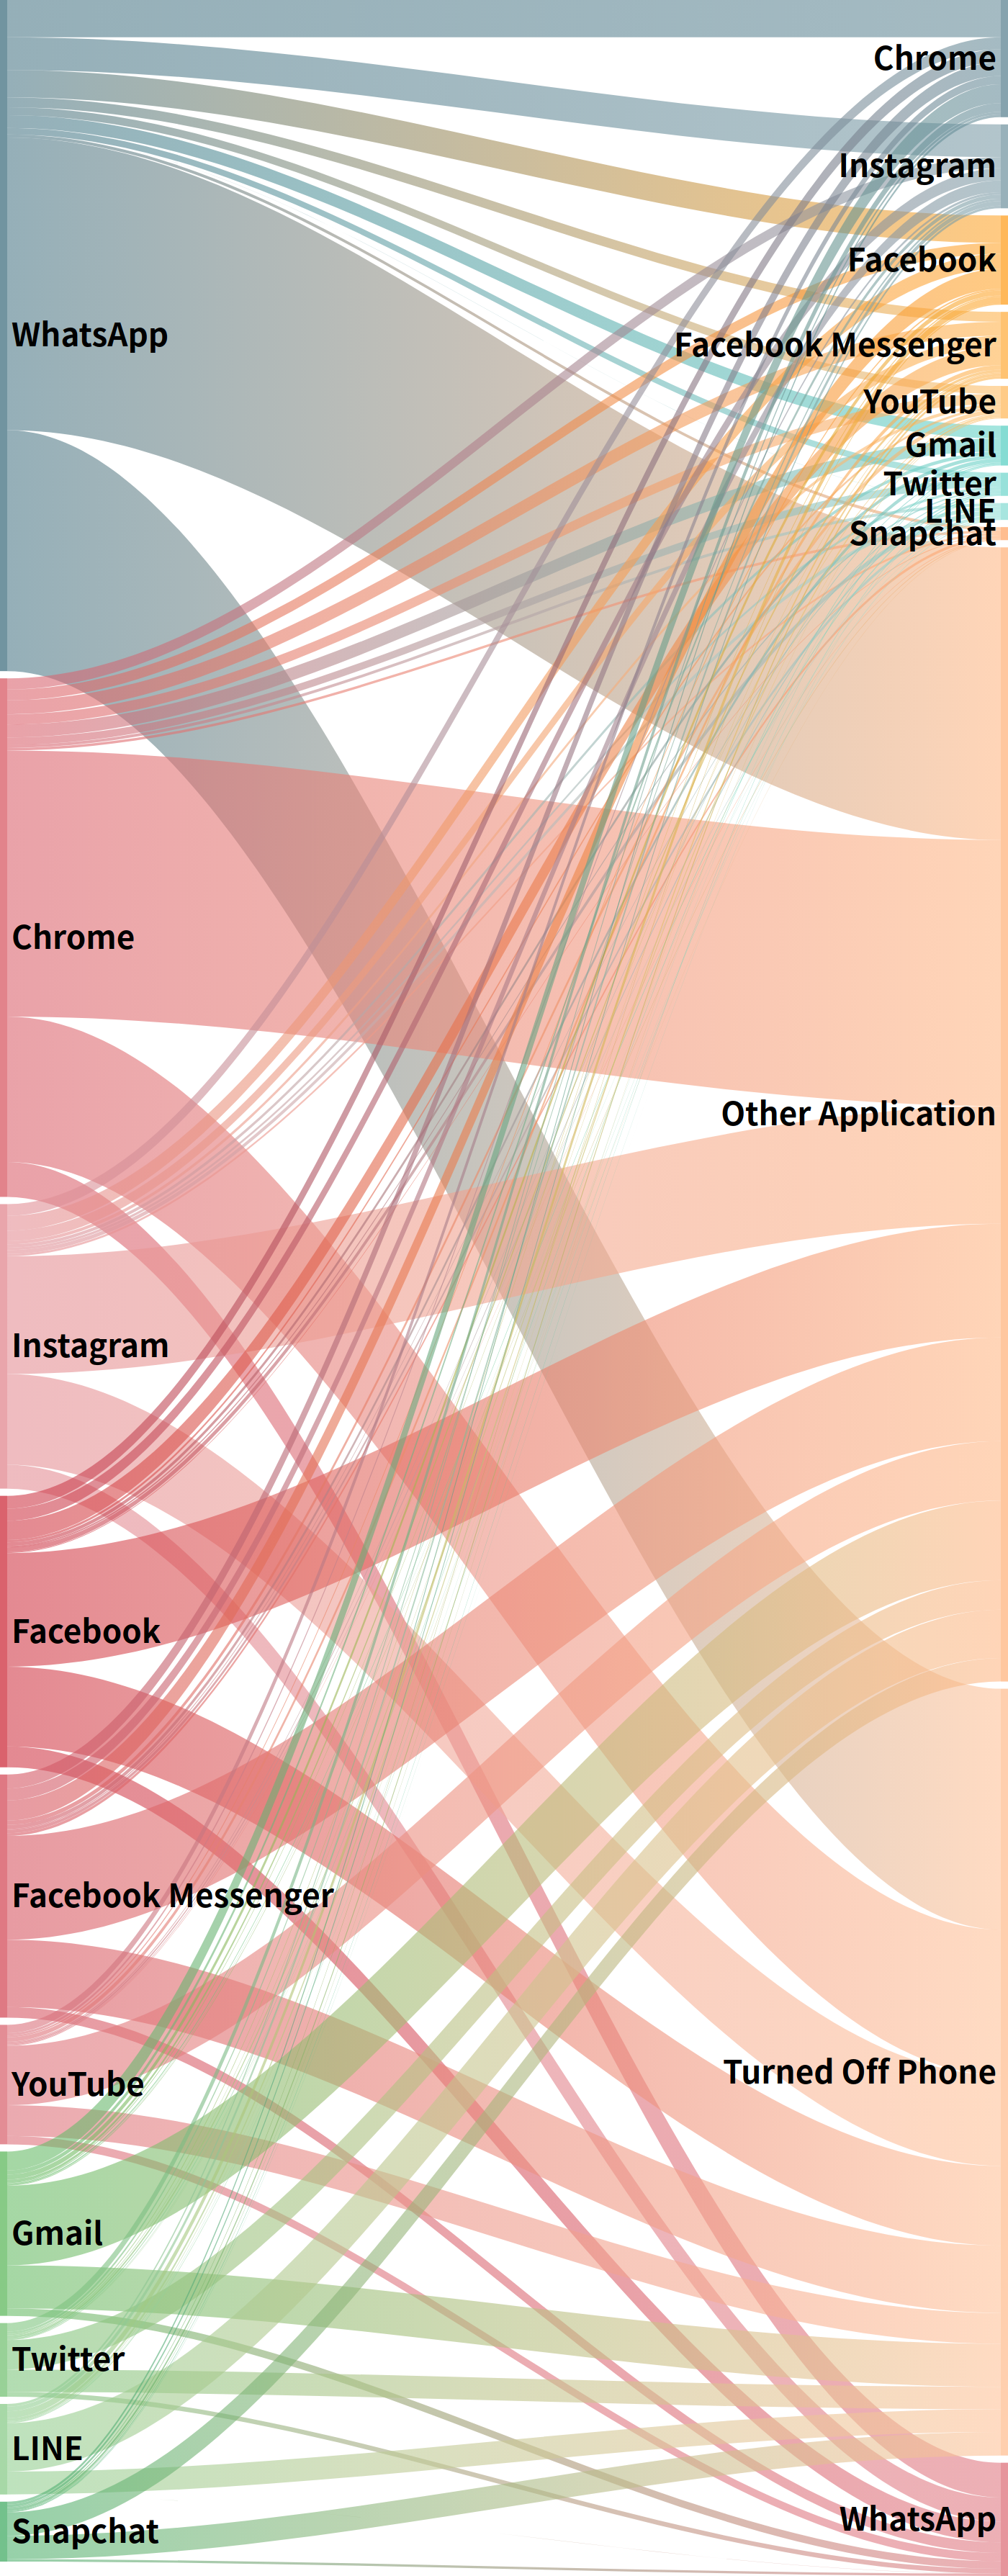
\includegraphics[width=\linewidth]{figures2/android_sankey_v7.png}
\caption{
%\zilin{Maybe the fonts are too small?}
The top 10 goal apps with the most number of sessions on mobile are on the left. On the right is the distribution of where a user ends up immediately after.
%\msb{text is too small to read. Double the font size. Cut some if you need to.  rule of thumb: figure text should never be smaller than the body text of the paper.}
}
  \label{fig:android_sankey_v2} 
\end{figure}

\msb{these figures are going nuts!!! can you fit them on the page?}

\begin{figure}
    \centering
    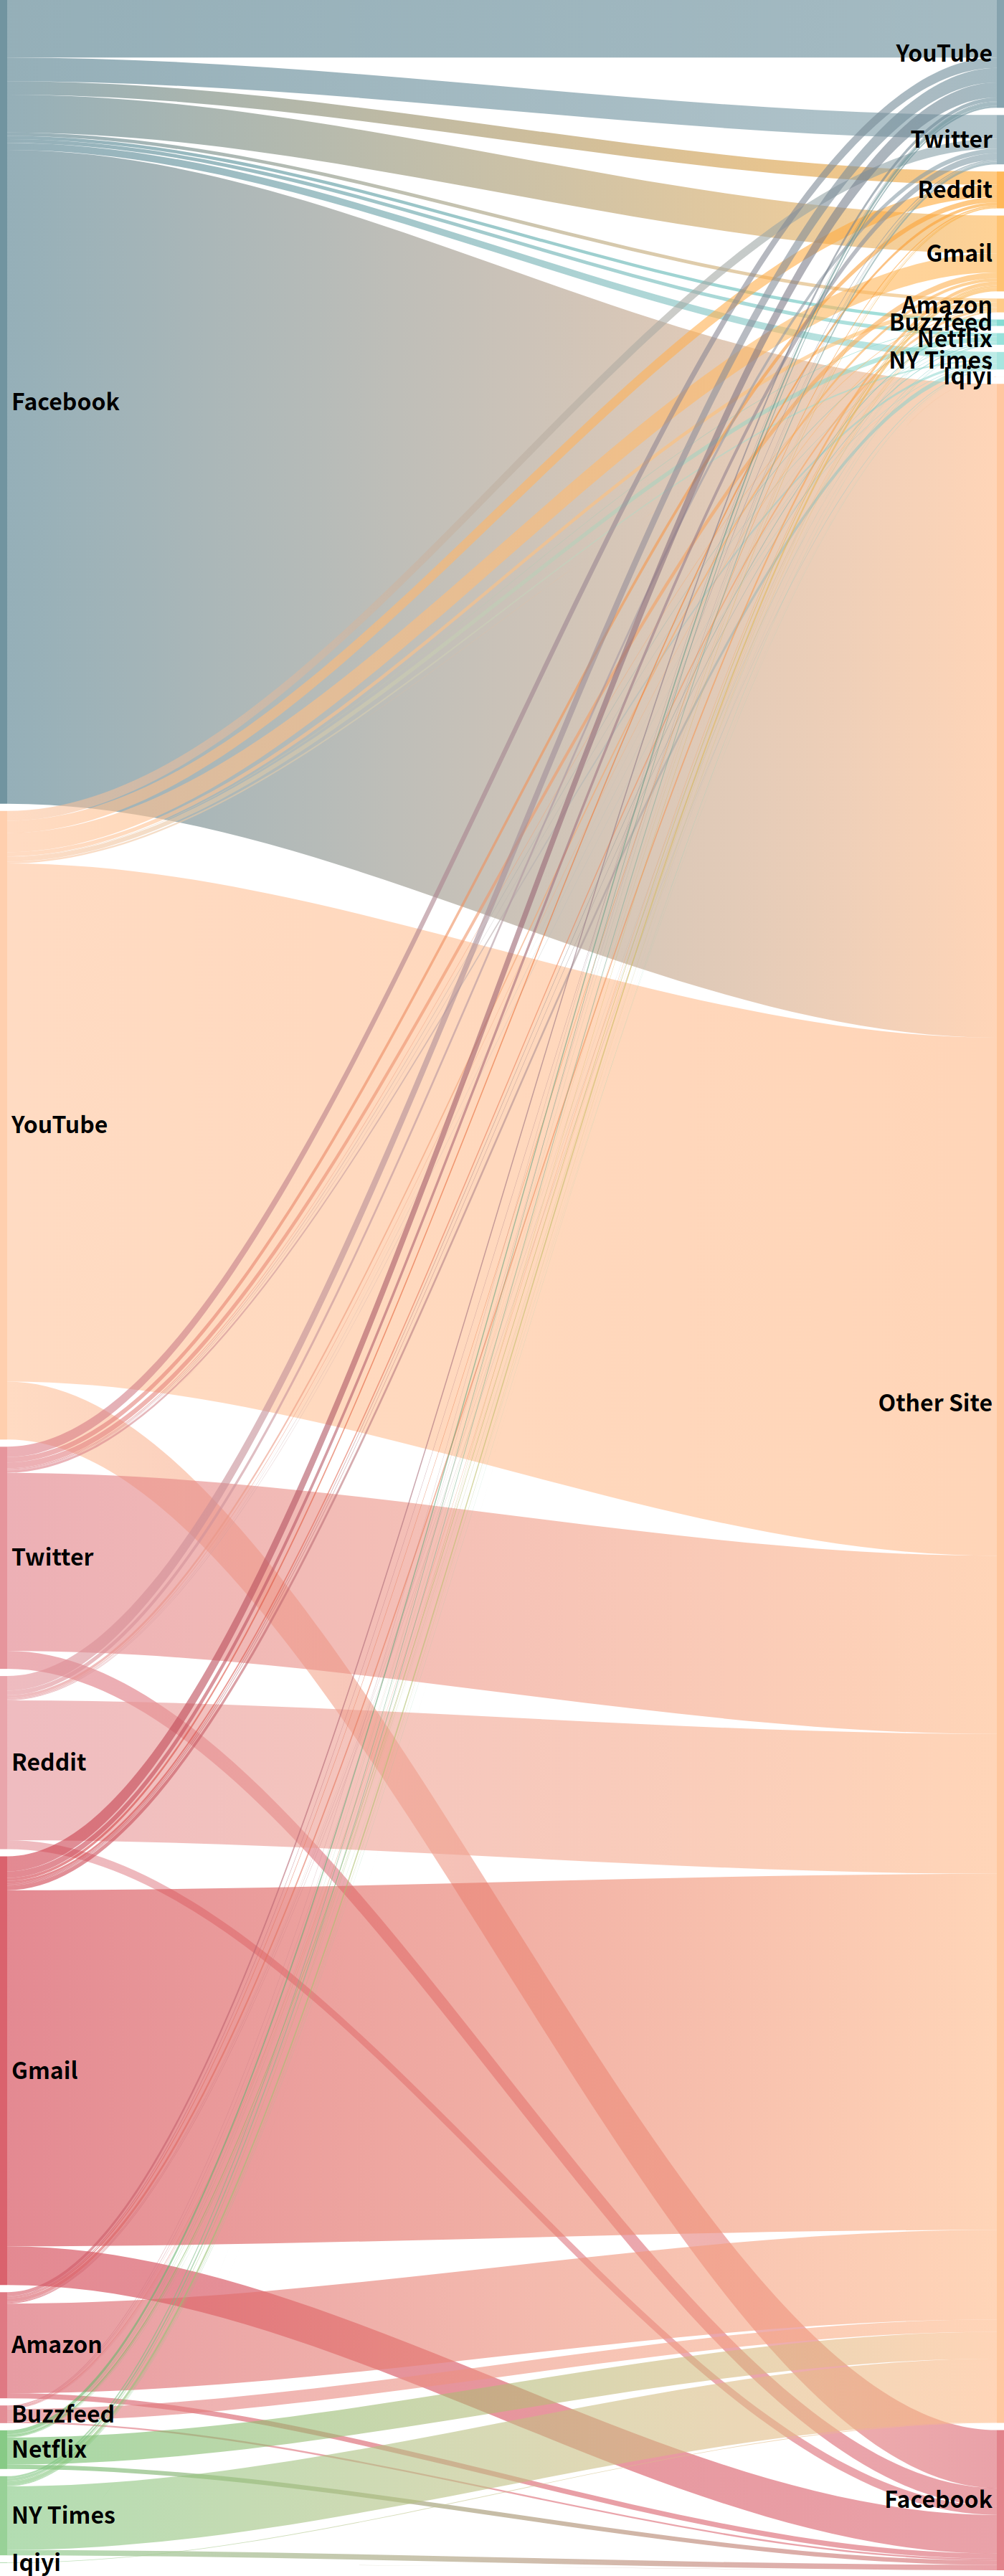
\includegraphics[width=\linewidth]{figures2/browser_sankey_v7.png}
    \caption{The top 10 goal apps with the most number of sessions on the browser are on the left. On the right is the distribution of where a user ends up immediately after.
    %\msb{text is too small to read. Double the font size. Cut some if you need to. rule of thumb: figure text should never be smaller than the body text of the paper.}
    }
    \label{fig:browser_sankey_v2}
\end{figure}



Finally, to build intuition as to the mechanism by which the above effects are happening, we analyzed what happens after users their goal applications. We visualized the flow of sessions from the 10 most widely chosen goal apps and sites in our dataset as Sankey diagrams (Figures~\ref{fig:android_sankey_v2} and \ref{fig:browser_sankey_v2}). On mobile, a majority of sessions end up going to another application, followed by turning off the phone, as shown in Figure~\ref{fig:android_sankey_v2}. On browsers, the majority of sessions went to other sites, as shown in Figure~\ref{fig:browser_sankey_v2}. We can also observe differences in goals users choose on mobile as opposed to desktop -- on mobile, the most popular apps tend to be messaging apps, whereas on the browser they tend to be content aggregators. %These classifications of productivity are taken from crowdsourced user ratings we were able to extract from RescueTime. The majority of sessions end up going to another application, followed by turning off the phone.

%  in Figures~\ref{fig:android_sankey_v2} and \ref{fig:browser_sankey_v2} \msb{this is not the right place to reference the figures; they are results, not method. there should be a point in results where you are looking to these Sankey diagrams to explain what's happening, and the major takeaways from these Sankeys included in the body text}.

\section{Limitations}

Our methodology varied frequency of interventions, instead of comparing having interventions completely on vs completely off. This approach reduces the size of effects we can observe compared to having interventions completely on or completely off. Our approach is also sensitive to variance in the effectiveness levels of the interventions. Some interventions may be more aggressive than others and change users' behavior more drastically even with low frequency. This difference may alter time re-distributions due to varied frequency. % \msb{I don't know what difficulties of the interventions means in this context}.

We did not measure time spent on platforms that HabitLab does not support. For instance, HabitLab users may use Facebook on tablet devices, watch TV or engage in other activities that are considered unproductive aside from browsing on a desktop or on an Android phone. These behaviors may potentially change how time redistributed, but we are unable to track it. 

%There might be other long term effects that we did not observe, since the length of the deployment ($5.8$ weeks) is not long enough.
Additionally, our study explores time redistribution in the context of productivity. It is possible that this context may not generalize to other behavior change regimes.
% \zilin{done}
% \msb{Other limitations that could/should be mentioned:
% - untracked interactions. what if they checked facebook on a tablet or something else we couldn't see?\\
% - length of deployment (we may not see effects over extremely long periods.\\
% - sensitivity to particular interactions. we used frequency as a proxy for how aggressive habitlab is. but interventions differ in actual aggressiveness\\
% - we've only studied this in the context of productivity,  it's possible that these results might not generalize to other behavior change regimes
% }





\section{Discussion}

We found that productivity interventions on the browser also reduced time on sites other than the targeted sites, but there was no such effect on mobile or cross-device.

We believe the reason we observed reduction in time on non-goal sites on the browser is several of the most popular goal sites --- such as Facebook, Reddit, Twitter --- are filled with hyperlinks to other sites, and hence drive traffic to them. For example, if an intervention makes a user spend less on their Facebook feed, they are going to be less likely to stumble upon a New York Times article, hence the Facebook-reducing intervention may also reduce time on New York Times.
Part of this may be a difference in how mobile applications work, compared to websites. Several mobile applications embed a web browser so that even if the user clicks a link, it will open within the same app. For example, Facebook is one such app, so if the user clicks on a New York Times link within the Facebook app, it is opened within the Facebook app's built-in browser, so the time they spend reading that article will still be counted towards Facebook app usage.

One possible reason for differences between mobile and web is that the apps users choose to reduce time on in each two platform differ (e.g., messaging apps on Android vs. link aggregators on Chrome). 
There also exist differences in typical interaction styles (short, notification-driven sessions on Android~\cite{oulasvirta2005interaction}, vs. longer sessions resulting from self-interruption on Chrome). 85\% of the apps that Android users frequently chose to reduce time on are for messaging (WhatsApp, Instagram, Facebook Messenger, Twitter, LINE, Snapchat), where a characteristic interaction is receiving a message, unlocking the phone to read it and reply, then turning off the screen (as shown in Figure~\ref{fig:android_sankey_v2}). Thus, users would not be drawn to other apps during this interaction. In contrast, with the Chrome version, the most selected sites are Facebook, YouTube, Reddit, and Twitter, 75\% of which are aggregators of links to other sites. The number of daily sessions per app is also greater on Android, though sessions are longer on average on Chrome, and stopping using the browser after a session ends occurs less on Chrome. Thus, the browser-based interactions users were using HabitLab to reduce are not short messaging-driven spurts that end with turning off the screen as on mobile, but rather long sessions of surfing through link aggregators ending with going to another site. So, a proposed mechanism: interventions short-circuit browsing long browser-based sessions, but mobile sessions are already short. % --- so users direct themselves to the browser, which begins a longer session.
% : comparing Facebook on both platforms, it is a median of 3 on Chrome, vs 9 on Android

This work brings about implications for designing interventions. Namely, we should consider not only the immediate interaction and its immediately measurable effects, but its longer-term effects in the context of the broader workflow. For example, consider 2 interventions for Facebook: 1) asks users to return to the home screen, vs 2) asks users to turn off the screen. Assuming similar rates of compliance, we would expect that measuring the effects on time spent on Facebook in isolation will show no difference between them. However, if we consider that going to the home screen can lead to users opening other apps, we might predict that a holistic measurement that includes effects on other apps as well will prefer 2) over 1).
Or if designing interventions to reduce snacking, should we: a) ask participants to not eat anything until their next meal, or b) give them gum instead? While calorie intake from the immediate interaction would favor a), b) may prevent future snacking down the line.
That said, in many cases, interventions are indeed isolated in their effects, and can even have beneficial effects elsewhere. % \msb{but don't our results also show that in many cases, things are isolated? I wrote that into the abstract given the results. whatever the takeaway is, I think it should be consistent in the intro+abstract+here.}

% Although our cross-device analysis showed no significant effects, we observed an insignificant trend cross-device suggesting the direction of predicted by our redistribution hypothesis. A possible explanation for a redistribution effect would be that. However, given that we observed

% This redistribution of time, even if it is slight, suggests that behavior change paradigms similar to HabitLab may be less effective and require greater vigilance than we hoped.


% Why would productivity interventions \jake{on Android} have a symbiotic effect, reducing time spent on other apps, but on the browser have a redistributive effect, increasing time spent on other unproductive sites? One possible explanation is the differing nature of the two devices. Mobile devices are primarily used for non-productive purposes and entertainment, which we use in many short sessions throughout the day -- the average user glances 100 times at a screen per day (todo actual number, need citation). Desktop and laptops, in contrast, are used for longer periods of time -- office workers will often spend nearly the entire workday in front of their computer, and with increasing amounts of productivity tools moving online, much of the workday may be spent on the browser. Hence, the effect of an intervention nudging the user off a site or app may differ across devices. We hypothesize that on mobile devices, the user's reaction may be to simply turn off the device, but on the desktop, they may instead go to a different unproductive site, or briefly switch back to a productivity application, but later go to a different unproductive site because their innate desire to procrastinate has not yet been fulfilled.

% Of course, if an innate desire to procrastinate is the underlying force driving the redistribution we observed on the browser, why didn't observe this effect on mobile? After all, even if an intervention causes the user to simply turn off their phone, do they not still have that unfulfilled desire to be unproductive? Perhaps the time is indeed being redistributed elsewhere to other unproductive activities, but the nature of mobile phones as devices that we carry around us everywhere, rather than being confined to the desk, makes it harder for us to observe where the time is going to. Perhaps the interventions on mobile are redistributing time to offline sources of procrastination, such as more water-cooler chats with colleagues. Without being able to track our users' every move, we cannot be sure whether this effect of mobile productivity interventions is truly symbiotic, or if it is simply redistributing to sources of unproductivity we cannot observe.

% Yet another possibility is the environment in which the devices are used. Perhaps the desktop browser is used primarily in an office setting, where the alternative to leaving Facebook is to go back to work, making Youtube seem to be a much more appealing place to go to if the user is feeling unproductive. On the other hand, perhaps users are using their phones in inherently recreational settings, such as in a mall or at a party, so if the user turns off their phone as a result of an intervention, they have plenty of other distractions in their environment to keep themselves happy and unproductive, and so they feel no need to go back to other apps on their phone.



\section{Conclusion}

%\zen{in the related work section, i did not mention isolated effect / symbiotic effect. will this confuse our readers?}
%\msb{Throughout the thesis, be careful about saying ``in this paper''. This is a thesis, so your options are ``in this thesis'' or ``in this chapter''} \geza{done}

In this chapter we have compared three hypotheses for how productivity interventions influence time spent on sites, apps, and devices other than the ones they are targeting. Productivity interventions may have no effect on other goals (\textit{isolated effects}), they may cause time to be redistributed to other unproductive goals (\textit{redistribution}), or they may cause a reduction in time spent on other unproductive goals (\textit{reduction}).

We adjudicated between these hypotheses by varying the frequency of productivity interventions on goals that users set in the HabitLab browser extension and mobile app. When interventions were more frequent, users spent less time on their goal sites and apps, showing that the productivity interventions were effective. We also defined a metric of intensity that captures frequency of interventions within device, and investigated the effects of varying intensity of interventions for other apps/sites, on time spent on an app/site. The result differed by device: on the browser we observed a global reduction effect, with time on non-goal sites decreasing with increasing intensity of interventions. However, on mobile we observed no effect. We believe these differences are caused by differing usage patterns and platform differences: websites drive traffic to other websites via hyperlinks, but mobile apps try to keep users remaining on the app. %a symbiotic effect, with time on an app decreasing with increasing intensity of other apps. We believe these differences are caused by differing usage patterns: interventions on mobile are causing users to turn off their phones, but interventions on the browser are simply causing users to go to other sites.

% When analyzing the effects of varying frequency of productivity interventions across devices, we observed no significant effect. We can attribute this to either our sample size being small \msb{I discount that explanation; cut it?}, or that in the cross-device case the isolated effects hypothesis truly holds \msb{also seems like throwing up our hands. either give a serious attempt at explanation here, or just don't try.}.

%\msb{this paragraph seems out of date now too; reduction doesn't seem like a bad unintended consequence:}
We have shown that while productivity interventions can sometimes have effects on usage of other, non-targeted sites and apps, they are often isolated in their effects. Hence, when designing for behavior change, while we should be careful about our measurements and the possibility of unintended side effects, in the context of productivity interventions it appears that targeting individual productivity goals does not cause substantial negative second-order effects. % Hence, when designing for behavior change, we need to be careful about our measurements and it is good to take a holistic approach if possible: the effects on a particular targeted app or site that we observe in isolation are not necessarily the net effect it is having on overall usage.

% \msb{this paragraph seems out of date now too; reduction doesn't seem like a bad unintended consequence:} We have shown that productivity interventions can have unintended side effects on usage of other sites and apps. Hence, when designing for behavior change, we need to be careful about our measurements and it is good to take a holistic approach if possible: the effects on a particular targeted app or site that we observe in isolation are not necessarily the net effect it is having on overall usage.

% Hence, we have shown that productivity interventions can have unintended side effects on usage of other sites and apps. Sometimes, they are detrimental and redistribute time to other sites, but other times they are symbiotic and help improve productivity outside the particular app it was originally targeting. Hence, when designing for behavior change, we need to be careful about our measurements and it is good to take a holistic approach if possible: the effects on a particular targeted app or site that we observe in isolation are not necessarily the net effect it is having on overall usage.

%\section{Acknowledgements}

%This work was supported by a Stanford Human-Centered Artificial Intelligence seed grant. We thank the many users who have used and contributed ideas and feedback to HabitLab.


%\pagebreak

\section{Appendix: List of Browser Interventions used in this study}

% There are 27 interventions total: 7 generic interventions that can beused on all sites, 5 interventions designed specifically for Facebook, and additional ones designedspecifically for YouTube, Reddit, Twitter, Netflix, Gmail, Amazon, iQiyi, and Youku

The following is the list of interventions used for this study, showing the intervention name and description as seen by the end user.\\

Generic interventions that can be used on all sites:
\begin{small}
\begin{itemize}
    \item Minute Watch: Notifies you of time spent every minute
    \item Supervisor: Shows time spent on site at the top of screen
    \item Scroll Freezer: Freezes scrolling after a certain amount of scrolls
    \item Stat Whiz: Show time spent and visit count each visit
    \item GateKeeper: Makes you wait a few seconds before visiting
    \item 1Min Assassin: Closes tab after 60 seconds
    \item Bouncer: Asks how long you want to spend on site this visit
\end{itemize}
\end{small}
\vspace{2mm}

Facebook-specific interventions:

\begin{itemize}
    \item Time Injector: Injects timer into the Facebook feed
    \item Feed Eater: Removes the Facebook news feed
    \item TimeKeeper: Notifies you of time spent in the corner of your desktop
    \item No Comment: Removes Facebook comments
    \item Clickbait Mosaic: Removes clickbait from the news feed
\end{itemize}

\vspace{2mm}

Youtube-specific interventions:

\begin{itemize}
    \item Sidekicker: Remove sidebar links
    \item Think Twice: Prompt the user before watching a video
    \item No Comment: Removes comment section
\end{itemize}

\vspace{2mm}

Netflix-specific interventions:

\begin{itemize}
    \item Fun Facts: Gives you a fact and links an article on the effect of TV
    \item Alarm Clock: Asks the user to set an alarm before watching a show
    \item Stop Autoplay: Stops the site from automatically playing the next video
\end{itemize}

\vspace{2mm}

Reddit-specific interventions:

\begin{itemize}
    \item Comment Remover: Removes Reddit comments
    \item Mission Objective: Asks what you aim to do this visit and puts a reminder up
\end{itemize}

\vspace{2mm}

Youku-specific interventions

\begin{itemize}
    \item Think Twice: Prompt the user before watching a video
    \item Sidekicker: Remove sidebar links
\end{itemize}

\vspace{2mm}

iQiyi-specific interventions

\begin{itemize}
    \item Think Twice: Prompt the user before watching a video
    \item Sidekicker: Remove sidebar links
\end{itemize}

\vspace{2mm}

Twitter-specific interventions:

\begin{itemize}
    \item Feed Eater: Removes the Twitter news feed
\end{itemize}

\vspace{2mm}

Amazon-specific interventions:

\begin{itemize}
    \item No Recs: Hides recommendations
\end{itemize}

\vspace{2mm}

Gmail-specific interventions

\begin{itemize}
    \item Speedbump: Delays the arrival of new emails
\end{itemize}

%\vspace{3mm}

\pagebreak

\section{Appendix: List of Mobile Interventions used in this study}

All mobile interventions are generic, that is they can be used on any app.

\begin{small}

\begin{itemize}
    \item At it Again: Sends a pop up with your app visit count.
    \item Progress Report: Sends a pop up with today's total usage for a certain app
    \item Red Alert!: Sends a notification with today's total usage for a certain app
    \item Repeat Offender: Sends a notification with your app visit count
    \item All in All: Pops a dialog with the day's total time on the current app
    \item Back To Target: Suggests you to visit a target app
    \item Counting on You: Puts a timer on screen in watchlisted apps
    \item Man Overboard! Shows a dialog with your app visit count
    \item No Peeking!: Asks for confirmation before opening watchlisted apps
    \item Wait Up! Pause for 10 seconds before entering an app
    \item Your Better Half: Sends a pop up to go to a target app
    \item Look on the Bright Side: Dim the screen a little at a time
    \item Take Your Pick: Select how long you want to spend on an app
    \item The Final Countdown: On screen timer that closes the app when time runs out
\end{itemize}

\end{small}


The following interventions apply across the device as a whole, not individual applications.

\begin{small}
\begin{itemize}
    \item How Time Flies!: Sends a pop up message with current app visit length
    \item Knock Knock: Sends a pop up with your glance count for the day
    \item Long Time No See: Sends pop up with your phone usage for the day
    \item Call it a Day: Sends notification with phone usage for the day
    \item Easy on the Eyes: Sends notification with glance count for the day
    \item Hello, Old Friend: Sends notification with unlock count for the day
    \item The Clock is Ticking: Sends a notification with the current app visit duration
    \item En Garde: Pops a dialog with the day's total unlock count
    \item Hold the Phone: Show dialog with phone usage for the day
    \item Long Story Short: Pops a dialog with the visit time for the current app
    \item Quote reminder: Show quote upon opening app
    \item Time Reminder: Show dialog with phone usage for the day
    \item Take Your Pick: Select how long you want to spend on an app
\end{itemize}
\end{small}


%\chapter{Changes in Preferences over Time}

In order to be effective at helping users achieve their goals, behavior change must be aware of not just the goals themselves, but how motivated users are to achieve them. This chapter will discuss a set of studies analyzing the goals of users using HabitLab, and an analysis of how their motivation levels change over time.

Users are diverse and have differing objectives for using software. Even in systems such as HabitLab where explicitly state their goals during onboarding, as wanting to spend less time on the sites that they select, the degree and means by which they wish to achieve this reduction can differ. We observed evidence of this in our uninstallation survey, where some users indicated they were uninstalling because interventions were too easy, while others were uninstalling because interventions were too difficult.

%In this chapter, we will first analyze how 

\section{Introduction}

Getting the right level of challenge and difficulty in behavior change systems is a challenging question. These systems must decide how aggressive they are in pushing users towards the desired behavior. A mismatch between the user's desired intervention difficulty, and the intervention difficulty selected by the system, may lead to the system being less effective, or being uninstalled. This leads to a design question of how do we choose the appropriate difficulty for the user to trade off attrition versus behavior change outcomes.

A number of options are available in choosing difficulty. One is to allow users to choose their preferred difficulty. However, this suffers from the possibility that their preferences may change over time. Another is to assign defaults that will push them towards the desired difficulty. Yet another is to intelligently predict the optimal difficulty levels.

Choice architecture theories predict that defaults are beneficial .... user motivation declines .... users are initially overly optimistic

In our first study, we test whether user control is beneficial. Method results. What do they pick. We find they are overly optimistic because over time their choices fall.

In our second study we investigate the effects of random assignment and disregarding user choices.

In our third study we investigate how well we can predict the choices of user difficulty over time, and how frequently we need to ask to get a accurate prediction.

\chapter{Discussion}

Some discussion go here

\chapter{Discussion and Conclusion}

In this thesis we have proposed a paradigm of in-the-wild experimentation to gain insights about behavior change, and have created a platform, HabitLab, to realize this vision in the context of helping users reduce their time online and on their phones. We also conducted a set of studies on HabitLab which illustrate that we can make novel findings with the system.

Our design principles with HabitLab focused on maximizing user retention rates, which we believe helped us with growth. We did so by giving users control of their interventions, providing visually appealing and unobtrusive interventions, and avoiding intrusive surveys and experience sampling as much as possible.

A major advantage we had with the domain we chose -- online behavior change -- is that we could push our interventions automatically to users on every visit, without requiring any interaction on their part. This may be considerably more difficult to realize in other behavior change domains, where it may be more difficult to sense when the targeted activity is taking place. For instance, dieting apps unable to detect when the user is about to eat may require the user to explicitly open the app to indicate when and what they are eating, so different design strategies -- such as unprompted push notifications that some might consider to be intrusive -- may be needed for other behavior change domains.

The first set of studies we ran with HabitLab investigated whether interventions decline in effectiveness over time. We found that interventions decline in effectiveness if the same intervention is repeatedly shown, and that a strategy of rotating between different interventions can help improve the effectiveness. While this comes at the cost of increased attrition, most likely due to users having incorrect mental models, we can reduce this attrition via a simple design shown when a new intervention is introduced.

We believe that novelty is an underlying mechanism for the improvement in effectiveness we observed when interventions are rotated. This leads us to speculate: would it be a effective and practical strategy to scale up the number of interventions, so that we are rotating between interventions from a huge pool of hundreds of interventions? Or do the improvements in effectiveness that we can expect from rotating increasing numbers of interventions have limits? We speculate that increasing the number of interventions in rotation will have high initial benefits for the first few additional interventions, but will have declining benefits as more interventions are added, as the probability of repeatedly seeing a recently-seen intervention grows increasingly small.

The second set of studies investigated whether interventions that help save time on one site, app, or device influence time spent elsewhere. We found that on the browser, reducing time on one site has a beneficial side effect of reducing time elsewhere. We believe this is due to reducing time on aggregator sites that drive traffic to other sites. On phones, however, we did not observe any side effects of reducing time on one app on other apps. We also did not observe any cross-device effects.

The findings of this study have a positive tone -- we did not observe negative side effects of productivity interventions, which would have been predicted if users were using their devices to replenish willpower when exhausted. Perhaps one speculative explanation is that in the context of device usage, diminished willpower results in the user opening a site or visiting an app, but actually spending time on the site or app does not replenish this willpower -- only the initial act of opening the site or app does. This may have interesting implications if it is true in other domains as well -- for instance, if the user is on a diet and has a craving for doughnuts, would an intervention preventing them from eating a doughnut also suppress cravings for other fattening foods as well? If they give in to the craving, would stopping them after the first bite leave their craving equally satisfied as if we let them eat the whole doughnut?

Given we conducted these studies in the context of reducing time spent online and on phones, results may not necessarily generalize to other behavior change domains. That said, with our increasing ability to sense our environment via sensors in our phones, smartwatches, and IoT devices, many of the paradigms we used in HabitLab can be applied to other domains as well. For instance, in the fitness domain, if we can sense users' physical activity levels via a smartwatch, we can experiment with various interventions that prompt users to exercise by playing audio messages or sending notifications. This hypothetical in-the-wild experimentation platform for fitness could potentially work analogously to HabitLab, running studies to find intervention strategies that work well to increase physical activity levels. The increasing ubiquity of sensors in the physical world make this paradigm of in-the-wild behavior change increasingly realistic and possible in domains outside online behavior change.

There is a large opportunity for behavior change research through big data and crowdsourcing that has been under-explored due to the paucity of large-scale deployments of research systems. Could we predict which interventions will work well for a new user, before they even start using the system? Could we automatically deploy and test modified versions of interventions, to hill-climb our way to more effective ones? Could we enlist an engaged user community to come up with, generate, and test new interventions for the long-tail of behavior change goals that designers had never even thought of? These can be realized with machine learning and crowdsourcing techniques, but there have not been appropriate communities for an in-the-wild deployment. We hope HabitLab will provide such a platform to realize this vision of community-driven behavior change research  in the wild. % through self-experimentation.


\appendix

%\pagebreak

\chapter{Replication of Chapter 4, Study 1 Findings using Session Level Measurements}

%\msb{Appendices should go in the appendix of the thesis --- there are no appendices for individual chapters} \geza{done}

This appendix replicates the findings of Study 1 using an alternative method of analysis, looking at time on site per session rather than day.

Time on site per session is measured as the total time the user was actively using a site in a browser tab, from when they visited the site until they closed the tab. If the user switches tabs to a different site, the time spent on the other site is not counted towards the current session time.

To determine whether the user is actively using a target site, we use Chrome's internal definition of active -- the browser window and tab is focused, the computer screen is on, and there has been mouse or keyboard activity on the tab within the past minute. 
Because time data is not normally distributed, we adopt a common practice of log-transforming the time data prior to analysis.

% Time on site per day is measured as the aggregated time across sessions from midnight to midnight in the participant's local timezone. There was one session data point per user per session per web site, and one day data point per user per day per web site.

\section{Effectiveness of interventions over time}

The likelihood ratio test confirms that the number of times a user has seen an intervention affected the log of time spent on a domain per session ($\chi^{2}(1) = 6.69, p < 0.01$), supporting H\ref*{hyp:decreaseovertime}. Each time the intervention has been previously seen increased the log time spent by 0.05633 (Table~\ref{tab:effectiveness_sessions_alldomain_vs_num_days_same_sessions}). By exponentiating the log estimates, this translates into an increase of 5.8\% on top of a baseline 46 seconds per session for each additional time the user saw the intervention during the study. %Note that since the dependent variable is log time rather than raw time, this 15\% estimated increase is multiplicative for each additional day.

An alternative method of analysis, where we measure the raw number of times the intervention has been seen instead of the number of days it has been seen, yields the same results. Restricting analysis to just Facebook also yields the same results. %\msb{does an equivalent analysis at the day level yield the same results? otherwise why did we make such a big deal of having both session and day data? If we're going to report both, we need to report both for all studies. Otherwise we need to cut and use just one.}

% Table created by stargazer v.5.2 by Marek Hlavac, Harvard University. E-mail: hlavac at fas.harvard.edu
% Date and time: Wed, Apr 18, 2018 - 19:22:06
\begin{table}[tb] \centering 
  \caption{Within the static condition, interventions decline in effectiveness, with longer visit lengths with increasing larger number of days since it was first observed.} 
  \label{tab:effectiveness_sessions_alldomain_vs_num_days_same_sessions} 
\begin{tabular}{@{\extracolsep{5pt}}lc} 
\\[-1.8ex]\hline 
\hline \\[-1.8ex] 
 & \multicolumn{1}{c}{\textit{Dependent variable:}} \\ 
\cline{2-2} 
\\[-1.8ex] & Log time spent per session \\ 
\hline \\[-1.8ex] 
 Number of days the intervention has been seen & 0.056$^{***}$ \\ 
  & (0.021) \\ 
  (Intercept) & 3.826$^{***}$ \\ 
  & (0.143) \\ 
 \hline \\[-1.8ex] 
Observations & 1,007 \\ 
\hline 
\hline \\[-1.8ex] 
\textit{Note:}  & \multicolumn{1}{r}{$^{*}$p$<$0.1; $^{**}$p$<$0.05; $^{***}$p$<$0.01} \\ 
\end{tabular} 
\end{table} 



%\pagebreak

\chapter{List of Interventions used in Chapter~\ref{ch:rotation} Studies}

The following is the list of interventions used for the studies in Chapter~\ref{ch:rotation}, showing the intervention name and description as seen by the end user. As this study was run before the mobile version of HabitLab existed, these interventions are all for the browser version.

There are 27 interventions total: 7 generic interventions that can be used on all sites, 5 interventions designed specifically for Facebook, and additional ones designed specifically for YouTube, Reddit, Twitter, Netflix, Gmail, Amazon, iQiyi, and Youku

Generic interventions that can be used on all sites:

\begin{itemize}
    \item Minute Watch: Notifies you of time spent every minute
    \item Supervisor: Shows time spent on site at the top of screen
    \item Scroll Freezer: Freezes scrolling after a certain amount of scrolls
    \item Stat Whiz: Show time spent and visit count each visit
    \item GateKeeper: Makes you wait a few seconds before visiting
    \item 1Min Assassin: Closes tab after 60 seconds
    \item Bouncer: Asks how long you want to spend on site this visit
\end{itemize}

\vspace{2mm}

Facebook-specific interventions:

\begin{itemize}
    \item Time Injector: Injects timer into the Facebook feed
    \item Feed Eater: Removes the Facebook news feed
    \item TimeKeeper: Notifies you of time spent in the corner of your desktop
    \item No Comment: Removes Facebook comments
    \item Clickbait Mosaic: Removes clickbait from the news feed
\end{itemize}

\vspace{2mm}

Youtube-specific interventions:

\begin{itemize}
    \item Sidekicker: Remove sidebar links
    \item Think Twice: Prompt the user before watching a video
    \item No Comment: Removes comment section
\end{itemize}

\vspace{2mm}

Netflix-specific interventions:

\begin{itemize}
    \item Fun Facts: Gives you a fact and links an article on the effect of TV
    \item Alarm Clock: Asks the user to set an alarm before watching a show
    \item Stop Autoplay: Stops the site from automatically playing the next video
\end{itemize}

\vspace{2mm}

Reddit-specific interventions:

\begin{itemize}
    \item Comment Remover: Removes Reddit comments
    \item Mission Objective: Asks what you aim to do this visit and puts a reminder up
\end{itemize}

\vspace{2mm}

Youku-specific interventions

\begin{itemize}
    \item Think Twice: Prompt the user before watching a video
    \item Sidekicker: Remove sidebar links
\end{itemize}

\vspace{2mm}

iQiyi-specific interventions

\begin{itemize}
    \item Think Twice: Prompt the user before watching a video
    \item Sidekicker: Remove sidebar links
\end{itemize}

\vspace{2mm}

Twitter-specific interventions:

\begin{itemize}
    \item Feed Eater: Removes the Twitter news feed
\end{itemize}

\vspace{2mm}

Amazon-specific interventions:

\begin{itemize}
    \item No Recs: Hides recommendations
\end{itemize}

\vspace{2mm}

Gmail-specific interventions

\begin{itemize}
    \item Speedbump: Delays the arrival of new emails
\end{itemize}

\vspace{3mm}

%\pagebreak

\chapter{List of Interventions used in Chapter~\ref{ch:conservation} Studies}

% There are 27 interventions total: 7 generic interventions that can beused on all sites, 5 interventions designed specifically for Facebook, and additional ones designedspecifically for YouTube, Reddit, Twitter, Netflix, Gmail, Amazon, iQiyi, and Youku

The following is the list of interventions used for the studies in Chapter~\ref{ch:conservation}, showing the intervention name and description as seen by the end user.\\

\section{List of Browser Interventions}

Generic interventions that can be used on all sites:
\begin{small}
\begin{itemize}
    \item Minute Watch: Notifies you of time spent every minute
    \item Supervisor: Shows time spent on site at the top of screen
    \item Scroll Freezer: Freezes scrolling after a certain amount of scrolls
    \item Stat Whiz: Show time spent and visit count each visit
    \item GateKeeper: Makes you wait a few seconds before visiting
    \item 1Min Assassin: Closes tab after 60 seconds
    \item Bouncer: Asks how long you want to spend on site this visit
\end{itemize}
\end{small}
\vspace{2mm}

Facebook-specific interventions:

\begin{itemize}
    \item Time Injector: Injects timer into the Facebook feed
    \item Feed Eater: Removes the Facebook news feed
    \item TimeKeeper: Notifies you of time spent in the corner of your desktop
    \item No Comment: Removes Facebook comments
    \item Clickbait Mosaic: Removes clickbait from the news feed
\end{itemize}

\vspace{2mm}

Youtube-specific interventions:

\begin{itemize}
    \item Sidekicker: Remove sidebar links
    \item Think Twice: Prompt the user before watching a video
    \item No Comment: Removes comment section
\end{itemize}

\vspace{2mm}

Netflix-specific interventions:

\begin{itemize}
    \item Fun Facts: Gives you a fact and links an article on the effect of TV
    \item Alarm Clock: Asks the user to set an alarm before watching a show
    \item Stop Autoplay: Stops the site from automatically playing the next video
\end{itemize}

\vspace{2mm}

Reddit-specific interventions:

\begin{itemize}
    \item Comment Remover: Removes Reddit comments
    \item Mission Objective: Asks what you aim to do this visit and puts a reminder up
\end{itemize}

\vspace{2mm}

Youku-specific interventions

\begin{itemize}
    \item Think Twice: Prompt the user before watching a video
    \item Sidekicker: Remove sidebar links
\end{itemize}

\vspace{2mm}

iQiyi-specific interventions

\begin{itemize}
    \item Think Twice: Prompt the user before watching a video
    \item Sidekicker: Remove sidebar links
\end{itemize}

\vspace{2mm}

Twitter-specific interventions:

\begin{itemize}
    \item Feed Eater: Removes the Twitter news feed
\end{itemize}

\vspace{2mm}

Amazon-specific interventions:

\begin{itemize}
    \item No Recs: Hides recommendations
\end{itemize}

\vspace{2mm}

Gmail-specific interventions

\begin{itemize}
    \item Speedbump: Delays the arrival of new emails
\end{itemize}

%\vspace{3mm}

\pagebreak

\section{List of Mobile Interventions}

All mobile interventions are generic, that is they can be used on any app.

\begin{small}

\begin{itemize}
    \item At it Again: Sends a pop up with your app visit count.
    \item Progress Report: Sends a pop up with today's total usage for a certain app
    \item Red Alert!: Sends a notification with today's total usage for a certain app
    \item Repeat Offender: Sends a notification with your app visit count
    \item All in All: Pops a dialog with the day's total time on the current app
    \item Back To Target: Suggests you to visit a target app
    \item Counting on You: Puts a timer on screen in watchlisted apps
    \item Man Overboard! Shows a dialog with your app visit count
    \item No Peeking!: Asks for confirmation before opening watchlisted apps
    \item Wait Up! Pause for 10 seconds before entering an app
    \item Your Better Half: Sends a pop up to go to a target app
    \item Look on the Bright Side: Dim the screen a little at a time
    \item Take Your Pick: Select how long you want to spend on an app
    \item The Final Countdown: On screen timer that closes the app when time runs out
\end{itemize}

\end{small}


The following interventions apply across the device as a whole, not individual applications.

\begin{small}
\begin{itemize}
    \item How Time Flies!: Sends a pop up message with current app visit length
    \item Knock Knock: Sends a pop up with your glance count for the day
    \item Long Time No See: Sends pop up with your phone usage for the day
    \item Call it a Day: Sends notification with phone usage for the day
    \item Easy on the Eyes: Sends notification with glance count for the day
    \item Hello, Old Friend: Sends notification with unlock count for the day
    \item The Clock is Ticking: Sends a notification with the current app visit duration
    \item En Garde: Pops a dialog with the day's total unlock count
    \item Hold the Phone: Show dialog with phone usage for the day
    \item Long Story Short: Pops a dialog with the visit time for the current app
    \item Quote reminder: Show quote upon opening app
    \item Time Reminder: Show dialog with phone usage for the day
    \item Take Your Pick: Select how long you want to spend on an app
\end{itemize}
\end{small}

%\section{User-Contributed Intervention Ideas}
\chapter{User-Contributed Intervention Ideas}
\label{ch:ideas}

Here is a complete list of intervention ideas that users have submitted via HabitLab:

\begin{lstlisting}[breaklines]
1: Buzzfeed:   n ,

2: Generic: "In this [x] minutes on [site name]  you would have... [fill in the gaps]

3: Generic: Disable news feed on LinkedIn, my biggest time waster

4: Amazon: Given max, if user spent money>max remind him that is useless to go to Amazon!

5: Facebook: only allow access to facebook messenger page + only allow access to Events page

6: Reddit: Just break the computer

7: Generic: motivational quotes

8: Generic: confirmation before loading the page, with a certain time forcing you to think

9: Facebook: Remind us Facebook admitted that it has always been a data mining Co. Period...

10: Youtube: Nudge after watching X minutes of video

11: Generic: before opening the site, display a (personal) list of alternative things to do

12: Generic: mom simulator: timed popups, are you using site because <x>? do <y> instead

13: Twitter: remove cats, categorized very popular BS feeds such as Only in Russia or similar

14: Generic: Automatic redirects to a more useful (user chosen?) site

15: Generic: Slow your scroll speed the longer you are on the site.

16: Netflix: Set time for length on website, after that time length, close tab.

17: Generic: Monitorize time spent on internet at all

18: Generic: Count limit number of posts, shares, reactions, etc. basically 'acts'

19: Generic: Ask when site opened if its related to goal.Limit tabs #, Use pomodore. timebox

20: Generic: Delay any temptive idea to search ask does it really make a difference in ur lif

21: Generic: http://humanetech.com/

22: Generic: I can suggest much more if if you enable me to. I have lots of ideas

23: Amazon: A budget reminder, so people don't end up overspending browsing random items.

24: Generic: stops you visiting a selected site for a while after your first visit

25: Youtube: Every minute it would display the amount of data used by youtube.

26: Generic: As I prep for tests, I'd love to get encouragement to spend time on some sites.

27: Amazon: It will tell you how much you spent and if you spend over $50, it block Amazon

28: Generic: Nudges applied to all bookmarks. e.g. to justify my visits to favourite websites

29: Generic: Generate a social media post announcing how much time you've wasted and where.

30: Generic: an hourglass of the mins I have to live, and how many of them are spent online

31: Generic: Prevent me from browsing sites during certain times.

32: Generic: Disable or limit clicks on outgoing links on a page

33: Amazon: Donate money to charity on your behalf

34: Generic: I just need a tracker for a total time spent in the internet.

35: Generic: Could you please design a tracker for a tomal time spent in the internet?

36: Generic: I would like to b abl to change the size of the "timer". Current one is too smal

37: Nytimes: Limit to two (or N) links clicked from the homepage each visit (or per hour)

38: Nytimes: Warning before loading the site for the second time in less than an hour

39: Generic: Remind me I just opened/closed the same damn tab 7m ago. For the 14th time today

40: Youtube: play asmr videos only

41: Generic: Add a blurry overlay to the screen that gets worse as time goes on.

42: Generic: For a porn website, add popup memes during the videos.

43: Facebook: Close the tab after a certain amount of time

44: Generic: Goals reminder: reminds you of your goals to promote better decisions

45: Netflix: Prompt user to confirm if they wish to continue watching before next auto play

46: Youtube: Force video to take entire window (not fullscreen, just larger theatre mode)

47: Youtube: Force disable autoplay

48: Youtube: Restrict the number of links that can be followed in one session (Wikipedia too)

49: Generic: 1 thing that u need to do & 1 thing you wish you could do if u had more time

50: Gmail: Limit the number of refreshes to inbox before auto-logging out

51: Generic: A popup reminder of why this is important to you, e.g. "your novel is waiting"

52: Generic: How about tracking time spent in Incognito mode?

53: Gmail: Self-set timer - e.g. reminder every 30 mins

54: Youtube: Reminder triggered by start of new video or pausing video

55: Facebook: Force you to wait at least 60 seconds before a finished comment is posted. PLZ.

56: Generic: Ask what your goal is for the visit

57: Generic: Ask how much time you want to spend on a site before the tab closes

58: Twitter: Make notification updates non-live - e.g. once per hour / 2 hours

59: Buzzfeed: redirect to home screen or site of choice

60: Facebook: redirect to random wiki

61: Netflix: close page at end of episode or when paused

62: Gmail: apply to-do list with task-based timer

63: Generic: Prompt for hourly pay rate.  Express time wasted in dollars wasted.

64: Generic: display total weekly stats at top of page

65: Youtube: closes when the viewer watches a certain amount of videos

66: Amazon: Do you need what you are about to go here and look for? (any eCommerce, really)

67: Generic: Restricts how many times you can open a site. eg 10-20x (For me, a stocks site)

68: Generic: 1 minute assassin, but w/o stupid "add time" button. Clicking that feels amazing

69: Twitter: limit thread or hashtag to 2o tweets

70: Custom: limit comments to 1 page , or remove next page button

71: Facebook: Meditate: count n in breaths and n out breaths (e.g. n = 3-5) before entering

72: Youtube: Prevent constantly changing videos by showing a pop up

73: Generic: sync with Google Tasks (or whatever task manager), show what is due next

74: Amazon: A counter that shows the number of clicks...the number of items you've viewed.

75: Generic: Sentences like "In the time you spend here weekly you could learn X in Y weeks"

76: Youtube: Lock the video interface and then slowly turn down the volume

77: Generic: Spanish please

78: Facebook: Only show 3 posts from the newsfeed, no more.

79: Twitter: Only show 10 tweets and don't load any additional ones when you scroll.

80: Generic: Changing end-of-day from 12am to 4am would be better for me, still up at 12am.

81: Reddit: Ask "why did you visit Reddit"? (A) Share something (B) Break. (C) etc...

82: Generic: Scroll Reseter: Automatically scroll back to top of page after N scrolls.

83: Generic: Show link to some alternative website you could be spending your time on.

84: Generic: Disables clicking for the first 15 seconds on the website.

85: Generic: Delays 15 seconds between clicking a link and having that link open.

86: Facebook: Popup msg spend time with family and friends with calc time wasted(avg life - t)

87: Generic: Solve basic math problem

88: Generic: x min assassin aggregated per some webs (x set up by user)

89: Generic: A big text saying: You have some important things to do!

90: Generic: a large message appears blocking the screen content

91: Netflix: Ask you how many episode(s) you will be watching

92: Generic: Ask me: Is this educational?

93: Facebook: Remove News Feed for a Day

94: Generic: send a warning/stop after opening x number of links

95: Generic: nothing

96: Amazon: Ask the person if they NEED the product, or just WANT the product impulsively

97: Amazon: паотьшгопимрнготьргемсавукцчяфйотбдлтнпаапмирпне

98: Reddit: Selected subreddit- Only allow access to selected subreddits for a little time

99: Youtube: Prepare for IIT JEE, see only relaxation music and iit related lecturesvideos

100: Generic: Ask how much time I want to spend on the site, close the tab after time runs out

101: Twitter: Scroll freezer

102: Generic: An exploding burst of colour & glitter with text - time to go outside & play

103: Generic: An exploding burst of colour with the text 'time to go outside & play'

104: Amazon: Show a timer in the corner that says how much time you've spent browsing

105: Amazon: Count the number of products/pages you've clicked on since visiting the site

106: Generic: What is your spending limit for this website/purchase?

107: Generic: In general: offer sign in option first for extension, handy if more than 1 pc

108: Generic: Also, increase text limit nudge suggestion :P

109: Amazon: What you want to buy? And how much do you want to spend? And inject amount  cart

110: Facebook: Blocks specific Facebook functions such as Feed and spamming notifications.

111: Youtube: stops you from being able to watch a video after watching a set amount of videos

112: Generic: Remove instagram feed

113: Facebook: Set time that you want the browser to block your Facebook.

114: Generic: A video montage of people accomplishing things to show what you're missing

115: Generic: The screen turns blank every 10 seconds with a message

116: Generic: an updated list of things you could have accomplished in the time you've spent

117: Gmail: Limit or alert after 30 seconds on a "compose" screen. Emails should be short.

118: Generic: flip the screen upside down

119: Generic: Shake the screen (window) visually or temporarily black it out

120: Generic: A animated figure pops on the screen point to there watch and taps it.

121: Calm: Do something productive

122: Gmail: Read or Go for a walk

123: Youtube: Call a Friend

124: Generic: Not a nudge, but a timer so that this only works during work hours would be fab!

125: Generic: Combine with a pomodoro timer to make this a super productivity tool

126: Generic: Holy grail> an active hours function+pomodoro, that live syncs across devices

127: Twitter: hide retweets that are trending too quickly, as they're likely time-wasters

128: Amazon: Ask what I am specifically shopping for

129: Generic: darken screen; large timer in center. press "space" to leave; ESC to stay

130: Generic: Please make this for Firefox

131: Twitter: Put fake tweets into feed asking with increasing frequency, "Why are you on Tw?"

132: Youtube: videos play faster, or ads play slower, gets progressively worse

133: Generic: freeze keyboard controls until the tab is removed after a set period of time

134: Facebook: Ask you a group of peoples feed to show only (eg: just family)

135: Generic: 5 minute assassin option(similar to the 1-minute assassin nudge)

136: Generic: multi nudges at the same time

137: Generic: 5 minute assassin timer nudge(similar to the 1 minute assassin nudge)& show time

138: Generic: When I am getting off track from the original reason I went online. Surf time

139: Generic: Flip the screen vertical

140: Amazon: Logs you out after a set amount of time.

141: Generic: ask how scrolls I need to do to block it

142: Gmail: sticky note pop out on your screen and say girl or boy you have 5 mins left

143: Twitter: Pop up that says, "Haven't you already read this?" (News services, too!)

144: Facebook: Simple questions: Did you find what you were looking for? Still here? etc.

145: Generic: Plays an alarm sound every x minutes, for example every 10 minutes you hear it.

146: Youtube: show time spent on youtube

147: Youtube: que no pongan anuncios en pleno video(en medio) del video

148: Youtube: stop auto-play of next video - replace with a prompt/timer/reminder if possible

149: Amazon: ask what online to buy, how much time needed, then prompt when approaching time

150: Generic: Telegram

151: Youtube: Close after 1 hours

152: Youtube: Only show the videos you need

153: Generic: Timer but flashes every X seconds in diff parts of screen

154: Generic: if you visited a website for the 20iest time in the last 3 hours, block it

155: Generic: blank screen intermittant after said time

156: Generic: feedeater& thinktwice (bcz user get there with purpose, but feed wastes) quora,

157: Youtube: Block the tab at certain times that you can set up

158: Youtube: Is this for study or not ?

159: Youtube: Auto-pause a video after a certain amount of time and show your stats.

160: Generic: Pop ups every 5 minutes that remind you and ask if you should still be on there.

161: Generic: pictures to a meme or to a set picture which motivates people,like family pictur

162: Youtube: Receive a warning after spending some specified amount of time

163: Generic: Every min, flash screen off for 5 seconds and remind them their goals + accompl.

164: Youtube: At a certain time, set by the user, the video will start stutter.

165: Youtube: Classify the video title(fun/usefu) notifies user if he/she spents too much time

166: Generic: Make the remind/aim banner dark instead of white

167: Generic: Ability to set specific nudges on or off, I just like certain ones more.

168: Generic: Allow control of consumption by amount of data spent

169: Generic: For all websites, ask how long you want to be on the internet for all together

170: Youtube: Detect "Recommended" browsing and how many videos you've hoped on a row

171: Youtube: Click (twice or let users wait) to show the video recommendations on the side

172: Facebook: Ask math question before opening site.

173: Generic: Linkedin


174: Youtube: Get rid of sidebar

175: Twitter: For a certain time frame, have only a certain subset of tweets appear on feed.

176: Twitter: Tick down the # of links, replies, etc. you click on then freeze for some time.

177: Facebook: Hide repeteated posts or hide posts that has been already displayed

178: Generic: Ask to stop or close tab

179: Generic: Higher Self. Display a prompt encouraging user to reflect on values

180: Generic: Link Lock: Sets (x) amount of links/videos user can click per day per site

181: Generic: The time wizard, but non-intrusive. The Mission Objective, but on specific sites

182: Youtube: Vomiting audio

183: Generic: Vote if tab "created idea" or "killed time" on close; report ideas by tab title

184: Facebook: I want the few second delay just for facebook

185: Generic: A notification to bring user back to the browser and stop surfing offline files

186: Generic: Go to bed (with insomnia option)

187: Amazon: Asks you what you are here to purchase

188: Reddit: Shows only the top 10 threads in the 'popular' section

189: Facebook: hide news feed

190: Generic: Personalized messages on screen (ex. "Don't you want to go to medical school??")

191: Generic: Change all images to Nicolas Cage face (Like chome's ncage extension)

192: Generic: every minute, the webpage becomes gradually more pixelated

193: Generic: Put links into a „TODO”-like list instead of opening them. This helps focusing.

194: Generic: After a configurable amount of time, close website and don't let me reopen it.

195: Generic: „Lock to this page”
Helps focusing on learning material. Block other pages.

196: Youtube: Limited amount of videos one can watc, as sometimes you need to watch for work.

197: Youtube: Block certain channels

198: Reddit: Remove the "next page" link on the old reddit, or block auto-scrolling on new

199: Reddit: Ask how many minutes to keep the tab open before killing it

200: Generic: pixels start getting blacked out

201: Reddit: Show only the first page of each subreddit and hide (or show less)

202: Generic: Time limit for a group of websites eg 10mins all social media, then no access

203: Buzzfeed: for them to stop being feminists

204: Ted: stop

205: Duolingo: learn spanish or die

206: Facebook: hello fellow white mothers

207: Facebook: HabitLab could post amount of time spent and visit count on FB wall

208: Generic: Progress bar that moves forward as user is productive and backward when not

209: Youtube: Turn off the sound for youtube/Pause the video, or put the video in slow motion

210: Youtube: Pauses the video and reminds you of a previously set reminder.

211: Youtube: Make a list for how much time you want to spend on each site and be reminded

212: Netflix: Shows you how many hours you have wasted on that particular show

213: Netflix: Close tab after preselected numer of episodes watched

214: Netflix: Lock episodes for series to one per day

215: Generic: Break time - set your timer for your break between tasks

216: Amazon: Shows your monthly/weekly/yearly purchase history dollar amount $$$.

217: Amazon: Removes Buy buttons, replaces them with Add to List so you have to wait & think

218: Youtube: Ask to minimize tab, so user can just listen not watch (for music or talks)

219: Buzzfeed: Tells you that you have better things to do and after that close after 60 second

220: Generic: Ask how are you feeling right now? or Is there a task you are avoiding?

221: Generic: Could you use a break - get up and take a walk.

222: Generic: Turns the entire screen white gives you a life quote and asks to continue

223: Twitter: Show only your notifications; clicking on any links force-closes Twitter.

224: Generic: Switch to 1st tab in browser window after specified time.

225: Generic: Mindfulness popup, after specific time elapsed.

226: Generic: After a certain amount of time, asks what your purpose is for still being there

227: Generic: make it black and white

228: Twitter: Don't allow feed refreshes

229: Twitter: Set a max time allowed per day, week, month

230: Youtube: When a video finishes Can you remove suggestions or next video?Or even playlists

231: Generic: A pomodoro technique complement. Work 20' and get your 5' treat.

232: Youtube: Close after a certain amount of time and restrict access until you say

233: Youtube: mode music please

234: Youtube: mode music please

235: Gmail: (if enabled) remove the "new messages" icon from social and promotions tab

236: Duolingo: Mejor es aprender otro idioma

237: Duolingo: aprender

238: Youtube: Ask me before what type of videos I want to watch/block and work over this list

239: Generic: PowerUSE: Utility-Span-Expiry. State purpose, make estimate, agree hardstop end.

240: Youtube: Music only mode. Disable videos, but allow music. To listen while working.

241: Facebook: Include Facebook Messenger (www.messenger.com) blocking messages or a time limit

242: Generic: advertising videos goggle up my RAM, slowing my page loading. Stop them please.

243: Generic: Top-level comments only. Removes all reply comments.

244: Generic: Block access to the website for a period of time

245: Netflix: Remove Suggested Shows/Movies

246: Twitter: Remove Likes/RT for your Tweets and removes comments for other people's Tweets

247: Youtube: Hide the comment section. A total time-killer.

248: Generic: Mood Tracker

249: Generic: Describe mood before clicking on a website

250: Generic: If on a website for too long, play a recording of yourself saying other ideas

251: Generic: A reminder that the work won't disappear, but these other distractions can wait.

252: Youtube: Only show the top 5 comments (and 3 replies per comment).
\end{lstlisting}


%\section{User-Contributed Intervention Ideas}
\chapter{User Feedback on GitHub Issues}
\label{ch:github}

Here is a complete list of feedback that users left us via the feedback interfaces in HabitLab, where users agreed to be have them be publicly shared on GitHub Issues. We removed all examples with any identifying information. Many of these are associated with images and screenshots, which can be viewed by clicking the GitHub link.

\begin{lstlisting}[breaklines]
https://github.com/habitlab/habitlab/issues/641
Hi - I love your app, but I have a few suggestions / requests.



I think it would be great if there was the option for greater control to select multiple nudges to function every time. In my scenario, the website I want to control is Youtube. I use Youtube a lot whilst I'm working and being productive for various tutorials, downloading copyright fee assets and so on. However, the recommended videos often push click bait "trending" content at me, and having gone on Youtube to find a tutorial on solving a certain problem, you suddenly find your self 5 minutes into a "You won't BELIEVE what Gordan Ramsey says to this Chef" or similar rubbish. I'd really like to be able to use the Feed Diet, Sidekicker, Supervisor, and No Comment at the same time. I feel like your app has everything I need, but I can't use it all at the same time :) 



Best,

Ben

https://github.com/habitlab/habitlab/issues/639
The disabling of autoplay makes me skip the recap of Jane The Virgin. However, that series includes new information and new jokes in every recap, so I always watch each recap even if I've just seen the previous episode. With autoplay on I can't watch the recap even if I've just logged in to Netflix, and even if I'm "rewinding" back to the beginning of the episode each time. It skips it again.

https://github.com/habitlab/habitlab/issues/638
it keeps asking me "how much do you want me to bother you??" and i am tired of answering this question. very cool extension that i used for like a year but something seems to have gone wrong so now i'm uninstalling :(

https://github.com/habitlab/habitlab/issues/637
I really wish there was a setting where I could use a nudge on every website except what's on a whitelist, because I always find a new place to waste time.

https://github.com/habitlab/habitlab/issues/635
Is there a way to set a default level of "how aggressive" for sites we want to reduce time on instead of choosing each time we load the site? ie, if I'm in the process of pulling up facebook, I'm much less likely to choose "heavy-handed" etc in the moment than I might in a more clear-headed moment ahead of time

https://github.com/habitlab/habitlab/issues/634
Disabling HabitLab due to excessive CPU usage. Right now the Chrome browser's TaskManage, CPU usage column shows HabitLab using 10-15% CPU. Ouch! Adios!

https://github.com/habitlab/habitlab/issues/633
What about separating out Amazon from it's Kindle page (read.amazon.com) and it music page (music.amazon.com) because I enjoy listening to music when I type, and (sometimes) I read books on my Kindle from the website for work.

https://github.com/habitlab/habitlab/issues/632
You should be able to group sites and provide overall limits and timers across the category. For instance, Netflix and YouTube would be considered 'media streaming' allowing the user to set a goal of say an hour of streaming a day. Otherwise, I can personally see me spreading my viewing over multiple different websites to (pretend to) keep within the goals.

https://github.com/habitlab/habitlab/issues/631
It's annoying that it asks always what nudge I want, when you open a website. Please stop this!

https://github.com/habitlab/habitlab/issues/629
It's annoying that it asks always what nudge I want, when you open a website. Please stop this!

https://github.com/habitlab/habitlab/issues/628
I have told this app again and again that I want to turn off 2 nudges, freeze scrolling, and setting the number of minutes I want to spend on a website in advance. HOWEVER IT KEEPS COMING BACK and I am almost about to delete this despite loving ever other aspect of it. FIX THAT ASAP. OR don't say you can remove it if you can't.

https://github.com/habitlab/habitlab/issues/627
Hey! Would be nice to have displayed the total amount of time spent on the web. Great work, people! Thank you for making this :)

https://github.com/habitlab/habitlab/issues/624
When I click sign in to sync nothing happens. I closed and opened new tabs and such and its still not working so I can't sign in

https://github.com/habitlab/habitlab/issues/620
Youtube nudges not working as expected. Sidebar and comments turned on and showing normally. How many nudges can I active simultaneuosly?

https://github.com/habitlab/habitlab/issues/618
I want to see my history and detailed results for longer durations, such as weeks or months

https://github.com/habitlab/habitlab/issues/617
I came to Facebook to check notifications for events, but the scroll freezer hides the entire top bar. And the search bar too! I can't manage the events that I came here to manage. The other HabitLab stuff is good though!

https://github.com/habitlab/habitlab/issues/616
Love HabitLab so far! However, I am unable to log in on the extension. I press the button and it does nothing.

https://github.com/habitlab/habitlab/issues/615
Thank you so much. I downloaded this to track my work time ( work on social media) and stumbled across the feed diet during one of the random cycles on youtube. I have never felt my mind clear like that just by not having the feed!! amazing extension, the possibilities are

https://github.com/habitlab/habitlab/issues/613
Nudges should NOT cover the page, they should possibly push the whole page down by the amount of space needed by the nudge: 

most apps, like twitter and facebook, have their buttons at the top, and your nudges simply cover those and make the site unusable, so maybe one wants to do a quick action on the sites bar and leave, but the nudge bar is in the way, so one is forced to close the nudge to access the function of the site and get on with it. But then the nudge is closed

Another possible solution is give the option to hide the nudge for 5-10 seconds instead of 1hour, but I prefer to see how the behaviour changes if the site usability is unencumbered



Mission Goal Nudges should allow at least to see what the page you were opening was. The objective can't be defined if you have multiple tabs open and you can't interpret from the url what the content you wanted to open was. Ideally it will be as blocking as it is now...so that it is the only action you can do, but you should be able to see the background page through for instance a darker screen, or a "peek" button that hides the nudge on rollover and shows it again as soon as you exit the button.

https://github.com/habitlab/habitlab/issues/610
ნიკა

https://github.com/habitlab/habitlab/issues/607
Show total browsing time including those pages not in top 5.

https://github.com/habitlab/habitlab/issues/606
Password for settings page, and nudge turn off buttons.

https://github.com/habitlab/habitlab/issues/605
Option to hide „Turn off HabitLab” button.

https://github.com/habitlab/habitlab/issues/604
Please add an option in settings to hide nudge turn off buttons (so they can only be turned off from settings page).

https://github.com/habitlab/habitlab/issues/601
On sites like news.google.com and reddit.com, you can click on links that take you to long articles on other domains where you can spend a significant chunk of time. Habit Lab doesn't track such changes now but really should!

https://github.com/habitlab/habitlab/issues/597
I want to see results per week and month - and to be able to compare each week / month. Also, an option to choose which day the week starts

https://github.com/habitlab/habitlab/issues/594
My nudges are not working most of time.

https://github.com/habitlab/habitlab/issues/593
i would like to suggest maybe you can make another tracking nudge that only allows you to stay on a certain website and cant open any other tabs

https://github.com/habitlab/habitlab/issues/590
Hi there, 



Sometimes, habit lab seems to turn off and I have no idea why. I haven't seen any nudges on facebook in the past week, but I didn't change any of my settings. This is the second time I've had this issue (last time I had to reinstall habit lab to fix it). What's the best way to fix this?

https://github.com/habitlab/habitlab/issues/589
Add minutes, not percentages, so i can see how many minutes i wasted on certain sites!

https://github.com/habitlab/habitlab/issues/587
Banner says a different website than the one I'm actually on.

https://github.com/habitlab/habitlab/issues/585
It won't show nudges

https://github.com/habitlab/habitlab/issues/583
In general, I think the random is a good idea, but I quickly realize some of the random ones are ineffective for me. Rather than the random, it would be great if I could designate 1 feature for a particular website. For example, I know that facebook is a big time waster to me and moreso than others. I would love it if that was 1 one minute kick-off no matter what. Others (eg - Twitter) are less of a distraction for me, so the random wouldn't be as painful.

https://github.com/habitlab/habitlab/issues/577
For the past few days, it only seems to track YouTube for some reason. Is there a way I could fix this?

https://github.com/habitlab/habitlab/issues/576
Hello! I am not sure if I am understanding properly, but with the Bouncer nudge (my favourite), once you have done it once in a day it never triggers again. It would be good for it to ask every time I go to a site, how long I want to spend on it. And if I exit the site, it refreshes and starts again.

https://github.com/habitlab/habitlab/issues/572
Nudges will frequently not show up when I visit facebook. Why is this? I haven't accidentally turned them off.

https://github.com/habitlab/habitlab/issues/571
Banner is too large

https://github.com/habitlab/habitlab/issues/570
the nudges arent really working....i have visited facebook multiple times now, but not have been nudged even once. I have enabled all the nudges as to see which one helps me the best, but its not nudging at all.

https://github.com/habitlab/habitlab/issues/569
None of the nudges are showing up. I'm not sure how to track down the issue.  I've pasted the contents of the javascript console from a visit to YouTube here https://pastebin.com/ZyPYB2Tw in case it helps track down the issue. Does HabitLab not work alongside adblockers or ghostery or something like that?

https://github.com/habitlab/habitlab/issues/568
Thanks

https://github.com/habitlab/habitlab/issues/567
your "how should we handle this" modal thing disappears on most pages before any human brain can be expected to click the options

https://github.com/habitlab/habitlab/issues/566
The extension doesn't track subdomains of a main domain properly. Suppose I add xyz.com as a filter and then it directs me to abc.xyz.com, the filter doesn't provide the needed nudges. This can be helpful if implemented.

https://github.com/habitlab/habitlab/issues/565
HabitLab extension in Chrome is using a lot of CPU

https://github.com/habitlab/habitlab/issues/564
Please add a login option at the start of the onboarding process to pull down any sync'ed data. I use a number of browsing logins on a number of computers and don't want to have to choose the list of sites every time. Also, a 'logout' option would be good. Also also, an email+password login would be handy for those who don't want to use a google account for this (or who want to share tracking and prefs across work and personal browser sessions)

https://github.com/habitlab/habitlab/issues/563
I believe settings across similar devices (laptop and desktop versus tablet and smartphone) should sync.

https://github.com/habitlab/habitlab/issues/562
I would love it if it would give me a running tally of my total minutes spent in addition to the "Today's five most visited sites by minutes spent" Thanks and cheers!

https://github.com/habitlab/habitlab/issues/561
How much time did I spend on what tabs, last week? Where are the totals?

https://github.com/habitlab/habitlab/issues/560
Think twice nudge for youtube does not work.

https://github.com/habitlab/habitlab/issues/558
How do I sign in to sync after the onboarding process? (Sign in to sync didn't work when I onboarded)

https://github.com/habitlab/habitlab/issues/557
Why do I not always receive a nudge when I visit facebook, I keep compulsively checking, and hoping a nudge will remind me, but I don't seem to be seeing any.

https://github.com/habitlab/habitlab/issues/554
I used two computers. On both computers, I am logged into Chrome with the same account as well as logged into HabitLab.  However, my settings are not in sync.

https://github.com/habitlab/habitlab/issues/553
Can you make a whitelist version?

https://github.com/habitlab/habitlab/issues/550
how about running it in incognito mode

https://github.com/habitlab/habitlab/issues/548
Please add a whitelist for stricter management, so we add the sites we DO want to access.

https://github.com/habitlab/habitlab/issues/547
Feed Eater Bug-  if I have the feed eater feature enabled, every time I open facebook, there will be an alert window along the lines of "How aggressive would you like HabitLab to be in helping you reduce your time spent this visit?", which gets tiring when you have to open facebook a lot of times for personal matters (not time wasting stuff I swear)

Update: Actually ignore what I just said about the Feed Eater bug, even with the feature off the issue continues on.

https://github.com/habitlab/habitlab/issues/546
Feed Eater Bug-  if I have the feed eater feature enabled, every time I open facebook, there will be an alert window along the lines of "How aggressive would you like HabitLab to be in helping you reduce your time spent this visit?", which gets tiring when you have to open facebook a lot of times for personal matters (not time wasting stuff I swear)

https://github.com/habitlab/habitlab/issues/545
Feed Eater  Bug

https://github.com/habitlab/habitlab/issues/544
Please let me have the "Mission Objective" nudge on youtube as well! I feel like it's one of the most effective nudges and would really make me consider twice whether to watch youtube or not.

https://github.com/habitlab/habitlab/issues/542
I have nudges/goals turned on, but they aren't appearing on any of the sites I enabled them on.

https://github.com/habitlab/habitlab/issues/538
Sidekicker, and NoComments are not working on YouTube.com. They work on "Try now" mode, but when actually expecting it to run while browsing, it does not work. I can see see Comments and Side bar.

https://github.com/habitlab/habitlab/issues/536
nudge "1 min assassin" that decreases to e.g. 30sec assasin if you already spent 10 minutes on the domain

https://github.com/habitlab/habitlab/issues/533
have multiple slots for work times. eg : 8h00 12h00 and 14h00 18h00

https://github.com/habitlab/habitlab/issues/530
In the selector for picking work days to be active it's very ambiguous which color means on and which means off.

https://github.com/habitlab/habitlab/issues/529
It seems like I can't add my own nudge idea because the "site which this nudge will be used on" dropdown is empty.

https://github.com/habitlab/habitlab/issues/527
Copy-pasted the js source for a built-in nudge into the editor and ran it. Had unexpected bugs not present in the built-in version.

Copy-pasted habitlab/src/interventions/youtube/remove_sidebar_links/frontend.js at commit da2cf17 into the nudge editor and ran it. All the comments as well as the tile of the video get grayed out, left menu no longer shows up when clicking the button (three paraller horizontal bars on the top left corner). This doesn't happen when running the built-in nudge. (Running Chrome. Youtube in dark-theme mode.)

Shouldn't they behave the same?

https://github.com/habitlab/habitlab/issues/522
I want to be able to temporarily turn off nudges for a particular website. For example, I'm watching educational youtube videos, but still want to avoid other sites.

https://github.com/habitlab/habitlab/issues/519
I've only been trying this out for about ~10 minutes and so far everything is working very well. I'm extremely pleased with it. However, I have different nudges enabled for different sites, but some sites are showing me nudges that should be disabled for that site. For example -- I have the more hardcore nudges like 1-min assasin and scroll blocker (cant remember specific name, sorry) turned on for both Instagram and Facebook, but only the ones like the timer/supervisor/objective nudges for Reddit. I use Reddit for work-related things often so I just need to be reminded to stay on task moreso than being blocked from the website altogether. I just opened reddit and the scroll-blocker nudge is what popped up even though it's specifically disabled for that site. Does HabitLab need to cycle through all the nudges once before it starts to show only enabled ones, or am I missing something? I can simply bypass the nudge but that defeats the purpose of enabling the other, more useful ones on this site. Thank you!

https://github.com/habitlab/habitlab/issues/517
When I turn off for the day/for the rest of the visit, it would be nice not to have a modal to confirm : I need one more click to close it, and it's annoying. If I wan't to turn it off, then there is no use anymore to slow down my use of thoses websites. See https://modalzmodalzmodalz.com/ for help

https://github.com/habitlab/habitlab/issues/516
Even when switching the Scroll Freeze off, the feature is applied. It freezes the scroll on websites that aren't even restricted.

https://github.com/habitlab/habitlab/issues/515
Intervention editor does not deploy nudges on "run this nudge" button

https://github.com/habitlab/habitlab/issues/514
Facebook nudges are not being deployed

https://github.com/habitlab/habitlab/issues/513
The Bouncer nudge shows the "how much time do you want to spend on this site" message too briefly for me to make a selection. Then it moves on to the site and closes it (because the default time setting is 0 minutes).

https://github.com/habitlab/habitlab/issues/512
Start making font (and other content) fade to grey with each scroll. Slowly the font will become tougher and tougher to read.

https://github.com/habitlab/habitlab/issues/511
This is one of the most useful extensions when it comes to fighting web addiction. However, many of the nudges, such as the news eater for Facebook fail to work at some occasions. And most of them does not work when combined with other nudges. This often defeats the purpose of the extension entirely. Otherwise, I love the idea of having nudges, the pie chart for an overview and setting daily limits. In the meantime however, I will use News Feed Eradicator for Facebook, WasteNoTime and RescueTime instead.

https://github.com/habitlab/habitlab/issues/508
I don't want to see the timer counting how long I've been on sites that I don't wish to spend less time on

https://github.com/habitlab/habitlab/issues/507
If I can disable the activated nudges easily, then there is no need for this extension. changing habits must be forced by rules made by the user.

https://github.com/habitlab/habitlab/issues/504
My settings are lost once I close Chrome.

https://github.com/habitlab/habitlab/issues/503
signed in to synch,  but after sign in synch  not implemented

https://github.com/habitlab/habitlab/issues/499
Hello, I really enjoyed using HabitLab, however I noticed it is consuming 16 -> 21% CPU, even when it is toggled 'Off' or otherwise not in use while on. This is unacceptable so it is being removed from my system (MacOS 10.13.6)

https://github.com/habitlab/habitlab/issues/498
XXXXXXXX

https://github.com/habitlab/habitlab/issues/497
I no longer see the pie chart with time spent on each site. How do I get that back?

https://github.com/habitlab/habitlab/issues/495
The piechart is not showing

https://github.com/habitlab/habitlab/issues/494
For some reason, graph doesn't show.

https://github.com/habitlab/habitlab/issues/492
there is something wrong ,the site isn't tracking my activities

https://github.com/habitlab/habitlab/issues/491
i can't see my most visited sites, it's not working

https://github.com/habitlab/habitlab/issues/490
I can't see the pie chart on the extension or the web page.

https://github.com/habitlab/habitlab/issues/488
i need the same software for firefox , how can i do ? can you help me ? and send me an email ?

https://github.com/habitlab/habitlab/issues/485
the extension for chrome(my verison is:Version 68.0.3440.106 (Official Build) (64-bit)) keeps hiding my you tube videos, it seems like a bug due to still keeping the names of the pages on the screen.

https://github.com/habitlab/habitlab/issues/482
Sometimes input messages don't work. The Mission Control nudge will display without asking for the objective (reading "Objective: " at the top), and the Bouncer will display without asking for the time, defaulting to zero minutes and immediately displaying the "Close tab / Turn off Bouncer / Cheat for 30 seconds" choice. Doesn't seem to have occurred on any of the default recommended sites, only on sites manually added by URL or the extension icon.

https://github.com/habitlab/habitlab/issues/480
Instead of Scroll Freezer I would just love a permanent feed remover! Let the feed be only as long as the window instead of infinite.

https://github.com/habitlab/habitlab/issues/472
I have an idea for a nudge. I would like to be able to remove "likes" from Instagram so that I don't see the number of "likes"  I receive--only that people liked it or did not.

https://github.com/habitlab/habitlab/issues/471
why does it show that i am spending time on facebook when my account has been suspended.

https://github.com/habitlab/habitlab/issues/470
I'm really excited about using this site but I did notice that the voting at the bottom of the habitlab chrome extension seems against the purpose of becoming less addicted to sites.  What's to stop people from constantly voting about the best nudges other than adding habitlab itself, if possible to do, to the list of sites to spend less time on? Just seems a bit contradictory.  I like the idea of asking for peoples' opinion but I'd say cap it at maybe 2 or 3 votes per time using the extension.

https://github.com/habitlab/habitlab/issues/469
"bouncer" doesn't work when you open internal links from within a blocked page (such as a facebook comment thread from your notifications, a reddit crosspost, etc). WOuld be great if it worked!

https://github.com/habitlab/habitlab/issues/468
There should be the ability to white list specific website to encourage certain behavior.

https://github.com/habitlab/habitlab/issues/466
Too many notifications interrupt my thought processes.  Hiding clickbait? I'm all for that.

https://github.com/habitlab/habitlab/issues/465
Show Stats from Yesterday (or more days from the past)

https://github.com/habitlab/habitlab/issues/464
not working on feedly.com -

https://github.com/habitlab/habitlab/issues/460
(from geza) font is off in the goal suggestion interface

https://github.com/habitlab/habitlab/issues/452
I don't see any option for easily changing over to purely tracking purposes - I have to manually turn off (permanently) each nudge AS IT  HAPPENS in order to do this, and since this doesn't integrate across instances of chrome (all my machines), I think I'm going to have to do this for each location that I use Chrome in.

https://github.com/habitlab/habitlab/issues/451
(from geza) css for the suggest goals interface seems to be off here compared to other sites. shadow dom issue? also the gitter api seems to have changed breaking our report bug functionality

https://github.com/habitlab/habitlab/issues/446
I turned the restrict your time nudge off because it caps at 5 min. I like the idea, but it needs to be free form.

https://github.com/habitlab/habitlab/issues/444
When given prompts for which nudges I think would be better, I got presented with two identical options - write some code that skips the comparison when that happens? (Also, the widening of this feedback rectangle while typing is a little disorienting; fixed-width would probably look nicer.)

https://github.com/habitlab/habitlab/issues/442
Please add a 1 hour or 2 hour disable for the interventions, "rest of today" produces unwanted results if I click it at (for example) 1AM, I want it to come back on after a while but not 24 whole hours

https://github.com/habitlab/habitlab/issues/438
Is there an option to block the site completely?

https://github.com/habitlab/habitlab/issues/437
I wish there was an option to set a goal and get pop-ups etc just for using Chrome at all, regardless of the site.

https://github.com/habitlab/habitlab/issues/436
Prompts if you would like to watch again or not when using the loop feature. Very annoying when playing music in the background.

https://github.com/habitlab/habitlab/issues/431
how about a metric that would total the time online from various sites and compare that against the aggregate "budget of time" for all sites?

https://github.com/habitlab/habitlab/issues/429
It would be great to have positive nudges as well. For example, a screen that asks if you would like to spend time on a site related to something one intends to do more of (meditation, exercise, job search)

https://github.com/habitlab/habitlab/issues/428
This app is not tracking my activity anymore

https://github.com/habitlab/habitlab/issues/427
I want to spend LESS time on the nytimes

https://github.com/habitlab/habitlab/issues/416
There was something to remind me to visit important sites ,, where is that feature ?

https://github.com/habitlab/habitlab/issues/415
(from geza) regression in youtube pause videos intervention

https://github.com/habitlab/habitlab/issues/411
I'm trying to set the hours nudges are active via "only work hours." It won't let me set them also for my sleep hours! I would like the nudges active from 11pm to 5pm

https://github.com/habitlab/habitlab/issues/406
YOU GUYS ARE AWESOME! I love nudges. I love Stanford. This helps me so much. I wish everybody knew about it.

https://github.com/habitlab/habitlab/issues/404
Guys, I fuckingly love what you made! I send you all my gratitude for your wonderful product!

https://github.com/habitlab/habitlab/issues/399
Settings aren't synced between browsers



I installed the extension on Chrome and customized some settings. When I opened Canary Chrome, the extension was installed, but the settings weren't synced. It's possible that this is a problem with Canary, but my guess is that settings also aren't synced between Google Chrome on different desktop machines.



The ideal solution would be to have user accounts, so that once the extension is available on other browsers, your settings could be synced between them. But it would probably be much easier to rely on Chrome's syncing for the time being, which would provide most of the benefit. (People probably tend to use the same browser on different devices.)



Keywords: sync, synch, synchronize, synchronization

https://github.com/habitlab/habitlab/issues/395
No increase in time though I often visit the page I want to reduce time on

https://github.com/habitlab/habitlab/issues/389
You're telling me that I spent no time on FB or Youtube, when I definitely did. I've not turned off HabitLab, so how does your measurement system work? Are there any other Chrome extensions it doesn't work alongside with?

https://github.com/habitlab/habitlab/issues/386
I use lots of PCs and MACs and would like to see my HabitLab a rather cross-device, Gmail-based account. Thanks a lot for the great work.

https://github.com/habitlab/habitlab/issues/385
turned on for twitter - minute watch distracting / annoying, so turned on (?) "supervisor", turned off minute watch.  It doesn't take.  It still annoys.  I'm about to simply turn off habit lab as a result.

https://github.com/habitlab/habitlab/issues/384
tiny bug, every midnight it shows a popup about having accomplished my goals of the starting day which obviously of course not the case

https://github.com/habitlab/habitlab/issues/381
I've had the extension installed for a few days now, but so far it hasn't tracked ANY minutes on ANY website. Happy to provide a list of current/active extensions if it would help. My first instinct is perhaps "HTTPS Everywhere"?

https://github.com/habitlab/habitlab/issues/380
Timer stops sometimes

https://github.com/habitlab/habitlab/issues/379
It does not accurately track the amount of time spent on Netflix, unless you are moving your mouse around. It starts counting, but then pauses counting after your mouse hasn't moved for a few minutes - i.e. passively watching a video. It was unable to accurately track the minutes spent even though the timer function was on, and I was interacting with it by pressing "snooze" a few times.

https://github.com/habitlab/habitlab/issues/377
As an alternate to a addictive site, you should let people completely step away and engage elsewhere. The alternative to a website should not only be another website.

https://github.com/habitlab/habitlab/issues/376
I hope this add-on works with Chrome on incognito windows as well!

https://github.com/habitlab/habitlab/issues/369
At times I am using youtube for educational content and would be nice to submit pages as educational so they dont trigger any HabitLabbehavior.

https://github.com/habitlab/habitlab/issues/363
It appears that the clock does not accurately count time spent on Netflix when in full-screen mode. It begins counting, but then pauses.

https://github.com/habitlab/habitlab/issues/362
I'm loving HabitLab so far. An additional suggestion: I want HabitLab to play a distinctive sound when a nudge is activated. Noises can be annoying, but they can also be a powerful part of retraining our habits. The user should obviously have the option to silence HabitLab, but the sound option would be a big upgrade. I would be glad to help develop a sound (or array of sounds) that could be used for this.

https://github.com/habitlab/habitlab/issues/361
Please allow option to not turn off buttons, e.g. "turn off feed eater button". Ideally this is a global option across all extensions. Thanks! :)

https://github.com/habitlab/habitlab/issues/348
There should be a way to combine sites into the same grouping (i.e. smile.amazon.com and www.amazon.com, and to account for different parts of the site, such as music vs. shopping)

\end{lstlisting}


\chapter{Responses to Uninstall Survey}
\label{ch:uninstall}

The following are the free-form responses to our uninstallation survey. Some earlier feedback items may be missing, as we accidentally lost them during a server migration. We also removed or modified items that revealed the submitter's identity or personal information.

\begin{lstlisting}[breaklines]
1: It did not work (nothing was registered)

2: another testing

3: Times logged don't accurately represent engagement with the site, e.g. playing a video in the background while viewing a different tab didn't count toward time but leaving the youtube home page open and idle did.

4: Neighbor installed this to my computer without my consent!

5: because i want to

6: muy molesto

7: Looked like some nice options for streamlining sites, but it's actually a nanny. I don't need a nanny whining at me.

8: I reached my goal to reduce time spent on certain pages. Thanks folks!

9: Didn't seem what I was expected. Installed two minutes ago and removed it.

10: I wanted something to track all websites, rather than having to opt-in to each.

11: I was just worried, I mean it's standford and all, but a bunch of students tracking everything I do and all my browser history, that just felt too much of a price to pay

12: ';

13: I forgot that I already had another program that did essentially the same thing for the computer in general instead of just for this particular browser

14: ...

15: changed my mind

16: Translate in french please

17: surveys done

18: You covered up useful buttons.  Don't do that.

19: Installed for a study, now the study is over.

20: just wanted to track time spend on youtube

21: it wasn't working on tumblr.com

22: I noticed that I was going on imgur, youtube, facebook (my choice of addictive sites) more, after I had installed the extension. So, I'm uninstalling. I think the extension made me more conscious of the fact that I was visiting the sites, but maybe the rewards were making me go back to the site? I'm not sure.

23: This is Matt, just deleting and reinstalling for something

24: Look and feel weren't great, I feel like it annoys more than it helps.

25: I don't need it :P

26: Wasn't sure if it is effecting battery life

27: Setting page was continuously popping up despite filling the setting.
Settings kept on reseting to default, despite setting the facebook specific timers they kept on getting disabled.

This was causing way more distractions than facebook which is sad.

28: it was just annoying you out of not using sites, not convincing you to. It became like ads, they are always there. But you don't like them and turn them off with ad-block.

29: l should be 0 this time

30: Hello,
This is the web browser for my raspberry pi 3 b. I use  website such as youtube and reddit for information and programming advice etc e.g terminal and python info. I do not wish to use less of these websites while doing this. However on my phone and laptop I do want to use less of certain site, as I use those devices for socialising and fun but it has become rather consuming of my time. BTW Habitlab is great application I hope the team achieves what it set out to do.
Thank you kindly
Regards
Chris

31: I don't spend a lot of time on facebook or other social media.

32: Was awesome, but was making chrome really slow, i mean really slow!
Seems like you need to fix some memory issues.

33: don't need, just wanted to try it
thank you

34: I liked the interventions but not on every page change or load, that was just a bit too much. Also I couldn't work out how to disable the thumbs up gif that appeared when I closed a site I was trying to reduce use of. Now that was annoying. Otherwise though it's a cracking extension! Good stuff.

35: Just testing

36: does not fucking work, hiding the newsfeed in particular

37: I was bored with it.

38: Did not turn off when requested. Kept on nagging even when disabled.

39: Found out I have good habits already.

40: I often browse incognito and it does not pick that up. Not that it should.

41: "Click here to finish setting up HabitLab"
"Click here to finish setting up HabitLab"
"Click here to finish setting up HabitLab"
"Click here to finish setting up HabitLab"
"Click here to finish setting up HabitLab"
"Click here to finish setting up HabitLab"
"Click here to finish setting up HabitLab"
"Click here to finish setting up HabitLab"
"Click here to finish setting up HabitLab"
"Click here to finish setting up HabitLab"
"Click here to finish setting up HabitLab"
"Click here to finish setting up HabitLab"
"Click here to finish setting up HabitLab"
"Click here to finish setting up HabitLab"
"Click here to finish setting up HabitLab"
"Click here to finish setting up HabitLab"
"Click here to finish setting up HabitLab"
"Click here to finish setting up HabitLab"
"Click here to finish setting up HabitLab"
"Click here to finish setting up HabitLab"
"Click here to finish setting up HabitLab"
"Click here to finish setting up HabitLab"
"Click here to finish setting up HabitLab"
"Click here to finish setting up HabitLab"
"Click here to finish setting up HabitLab"
"Click here to finish setting up HabitLab"
"Click here to finish setting up HabitLab"
"Click here to finish setting up HabitLab"
"Click here to finish setting up HabitLab"
"Click here to finish setting up HabitLab"
"Click here to finish setting up HabitLab"
"Click here to finish setting up HabitLab"
"Click here to finish setting up HabitLab"
"Click here to finish setting up HabitLab"
"Click here to finish setting up HabitLab"
"Click here to finish setting up HabitLab"
"Click here to finish setting up HabitLab"
"Click here to finish setting up HabitLab"
"Click here to finish setting up HabitLab"
"Click here to finish setting up HabitLab"
"Click here to finish setting up HabitLab"
"Click here to finish setting up HabitLab"
"Click here to finish setting up HabitLab"
"Click here to finish setting up HabitLab"
"Click here to finish setting up HabitLab"
"Click here to finish setting up HabitLab"
"Click here to finish setting up HabitLab"
"Click here to finish setting up HabitLab"
"Click here to finish setting up HabitLab"
"Click here to finish setting up HabitLab"
"Click here to finish setting up HabitLab"
"Click here to finish setting up HabitLab"
"Click here to finish setting up HabitLab"
"Click here to finish setting up HabitLab"
"Click here to finish setting up HabitLab"
"Click here to finish setting up HabitLab"
"Click here to finish setting up HabitLab"
"Click here to finish setting up HabitLab"
"Click here to finish setting up HabitLab"
"Click here to finish setting up HabitLab"

42: i don't like this

43: i love this

44: Debugging (am at Stanford)

45: They are preventing me from adding youtube songs to my youtube playlists.

46: testing to see if server is up

47: Only need on my main computer, and way too many little notifications in the bottom right corner with no clear easy way to turn them off

48: Extensions worked for only 5 minutes (until I started to modify the settings).

It's now completer borked. Clicking on "Options" sends the browser in an infinite loop.

Too bad, this looked like a useful project.

49: no like interference in all

50: There was no way to turn off notifications in chrome

51: It does not have any auto sync features. because I use Multiple OSes that's why I'm having so much problem.
Please add auto sync features  of Habits.

52: Just was testing the app

53: I wanted a timer for every "domain", it can be good for stadistics of time..

54: gyguv

55: may cause lag

56: Catastrophic stability problems after installation; may be due to a different extension

57: Couldn't figure out how to turn off the "clapping" gifs that appear when leaving a website.

58: Dont need it on work computer, just at home

59: downloaded twice accidentally

60: this is my wasting time computerand i dont need it

61: would not tun off even after I "turned this off for today" when I tried and corrected it it told me it was already off. Also was set to only run during work hours, and never stopped on the evenings or weekends. Basically it did nothing but bother me when i wanted to be online, and never helped me curb the times i didn't. So utterly useless!

62: d

63: A cool concept! Unfortunately, I don't use Chrome that much so it is not very useful for me. A mobile application would work much better for me since I tend to procrastinate on my phone.

64: There was a very irritating bug with Klout.

65: I love the idea—but I'd like stronger nudges and better tracking of the time spent on each site.

66: I was interested in tracking my usage to start, instead of setting interventions that I may not actually be concerned about. Additionally, much of my "wasted time" usage is on mobile which this wouldn't help me track.

67: Made Facebook unusable. Which might be the point?

68: Someone else installed. Did not want it

69: Gave up

70: LAG.....

71: i'm chopping and changing computers too much...

72: The "goals achieved" notification was annoying, I disabled it and it still intervened

73: n

74: hjhjk

75: .

76: only test install, good apps guys, regards from spain wihout user anonymous from castila la mancha :)

77: Could not edit settings properly. Even though I removed Gmail from sites to avoid, I still got notifications.

78: Should be able to monitor all websites first automatically, and not only user defined sites.

79: Testing

80: i don't need it

81: I think it messes with the Google Play Music

82: aaaaaaaaaaaaaaaaaaaaaaaaaaaaaaaaaaaaaaaa

83: Made me realize I don't have Facebook addiction, spending less than 30 minutes of my desktop time on it per day.

84: ./'l

85: Would have preferred a gentle log - perhaps emailed - giving usage statistics. In the present form this operates like pop-up ads. Still, it was reasonably insightful into understanding my usage for the time I used it. Thanks.

86: So

87: Seeing if this extension is causing gmail compatibility issues

88: Creating an intervention (such as temp_intervention created in the tutorial) does not seem to work at all. I'm reinstalling immediately to see if that fixes it.

89: I prefer the "Forest" application.

90: kept telling me 8/8 achievements complete when in reality I had not.

91: For some reasons Facebook blocked me and I am trying to figure out the reasons. What I know that the Hitlab extension was deactivated (not by me) and then, boom, I was blocked.

92: Software was buggy

93: all good

94: did not appreciate the clapping people. had issues with google music and now checking if an extension is the cause

95: not sure I really neded it - mostly use facebook and youtube for technical research and discussion. Good idea, though

96: disturbing gifs

97: I just don't use my laptop as much as I thought would be necessary for an intervention.

98: Not interested

99: I rarely waste time on my desktop. This would be much more useful on my mobile phone.

100: not what i was looking for in software.

101: Interventions are not forceful enough. They are too easy to click around or disable.

102: realized not spending as much time on websites as i thought...

103: хэ

104: Uses a lot of CPU and memory without doing anything

105: Mostly it was the bar covering up facebook message indicators.

106: Unable to change settings that appear in startup.  I couldn't find a way to set one type of nudge for all websites. It is really annoying to change settings for every single website. Hence reinstalling it.
One good feature will be to create a group of websites with similar nudge settings!

107: settings changed on me all of a sudden with caue and i got sick of going back over settings over and over to turn things off.

108: I like all or nothing.

109: It's quite possible something else was causing lag -- but lag there was.  I also was just checking it out.  I don't really use facebook or youtube.

110: I figured out that I actually don't spend as much time as I thought I was. I thought I was watching videos for 4 to 5 hours a day, but the timer stated only watch them for 30 minutes.

111: Not only annoying but they cover up important part of the screen

112: sucks

113: Cause Facebook news feed to constantly refresh itself so I was unable to read or click any links there.

114: I used the extension to curb my Facebook habit and eventually gave up Facebook altogether- something I've been wanting to do for a long time.  Thank you.

115: no need

116: Don't need it

117: I do not use it anymore

118: non lo voglio

119: My youtube doesn't work becauseof it

120: battery use

121: I love the app - I'm just removing temporarily to see if it's affecting another app (Freedom.to)
Thanks

122: I'm weak....

123: tuke

124: I'll be back soon

125: I just didn't understand the concept before downloading and it's intentions aren't my demons as it happens.

126: became unusefull for me;
good initiative any how

127: NA

128: Extension did not work as expected and I was experiencing bugs

129: I want to try other types of chrome extensions to block time-consuming websites and don't want to mess with your data.

130: performance... seems to use a lot of CPU all the time...

131: THis extension was causing system wide lag

132: I use social media for work - but your app is great and I will keep it running on my personal accounts

133: Por enquanto não preciso desse tipo de ferramenta no meu navegador.

134: Daily results show 0 time spent for almost all sites, despite that definitely not being the case.

135: excessive battery  consumption

136: All it took was the fact that settings don't sync, so I would have to reconfigure for each instance of Chrome.

137: Very Good, but want to reduce installed extensions.
Might install again later.

138: Spend too much time on the relevant platforms for work purposes.

139: dcsdf

140: Blocked usage of 1Password extension, which is critical.

141: 1

142: lags and bugs

143: Time spent differs drastically

144: wanted to install it on my private profile, not my work one.

145: just checking it out

146: dssd

147: I think I misunderstood the point of the program.

148: The Youtube sidebar still loaded.

149: didn't really need it. Turns out... I don't really binge watch after all.

150: No use

151: I need something mor physical, i can be distracting out of my computer

152: ijgougoughu

153: Consumes too much CPU

154: On Facebook, I couldn't click on regular posts (not just clickbait posts) that I truly wanted to see. So I disabled the clickbait feature and it was still happening. Then I disabled the whole app, but it's STILL happening. So now I have to delete the whole app to see if this fixes the problem :(

155: cxsd

156: nnfgnfgnngfnfntdrsxnrtsynr.shrehmsortihmnsrth,rtesmhposritmh[oimaerg][ognm[o9trignjm3io[54ny9ui35y-

157: Not effective for me - the interventions just slowed down my procrastination and made it take longer unfortunately! :)

158: its stupid asl

159: Basically just irritating.

160: I like what you are doing and see a great purpose. but when I was on certain pages the pop up from habit lab was in the way of seeing what I wanted to look at and then I felt frustrated and somewhat invaded......  due to the fact that I thought I had shut it down and then somehow it was on again. 
perhaps there is a quick habit blurb.... about how to shift when you get stuck on the computer etc, or using triggers to support positive habits or kaizen, 
If it is purely research base maybe there needs to be finessing around how the habitlab pops up or the look of it, it's placement on the site..... right now it feels slightly naggy, perhaps it could feel supportive in the look and placement of it. Like I said .... I like what you are doing.... It's super smart and hopefully will help gather  the  data you are looking for.

161: Didn't seem to work

162: Kept me off Facebook, but was not smart enough of a tool to know when I needed to check a message versus just idling

163: Used it over my study period, don't need it anymore. Thank you for it!

164: gmail and youtube stopped loading

165: seems cool but i feel its too intrusive, probably helps others who sit on facebook all day

166: Interfers with printing emails -- pops up as if one wants to print it

167: reinstalling so i can see the habitlab panel, not finding how to access this normally?

168: I was hoping for an analysis of my internet activity. This seems to be designed solely for the purpose of reminding users of youtube and facebook time.

169: Does not remove youtube sidebar and comments section

170: Caused interruptions when listening to youtube in the background. Many videos would randomly give an error and refused to be played about 30 or so seconds in.

171: I achieved my goals

172: It gave me the info I needed

173: it reached its goal as I am more cautious about my net usage

174: Didn't catch any website anymore

175: need to reinstall

176: Needs to synchronize stats between machines, ineffective otherwise.

177: I deleted the wrong one

178: Installed, because I was curious. I don't have issues with wasting time in the Internet.

179: i dont actually spend too much time anywhere so after trying it for a few months (i think?) its rly just annoying. but if you do have an issue with going on facebook or reddit (or whatever) too much, i'm sure its very helpful. if that ever happens i'll reinstall it :)

180: On one of my other synced devices (RCA Tablet 10.1 w/windows 10 new April 2018 ver.) it keep crashing and literally giving me a Black Screen of Death. It would just go bank and one time it did ask if I wanted to submit a crash report all other times the error was not scene just would not work.

181: Wasn't using it

182: fuck useless, useless team

do better things with your life

183: xzy

184: I clean toolbar and delete all extension

185: I feel it does not effective.
Rescuetime works better for me.

186: only need on work computer

187: a

188: No instructions on how to use it.

189: Was not effective at all. Provides a false sense that something is being done, making the problem worse. StayFocusd will do well to block these sites in their entirety rather than try to alter the design that tech giants spend billions perfecting.

190: ;not finals anymore!

191: wr

192: I wanted to crush my laptop's screen every time a stupid high five you saved a minute fucking awful meme was making an appearance cool marketing of extension but treating me like a stupid mindless kid is beyond annoying .

193: I needed to get rid of the Ram Chrome was using.

194: interventions overlay makes webpages unusable

195: I couldn't find how to de-select some (already selected) web pages.

196: Ticker blocked screen content

197: i will be back

198: hgh

199: ram usage

200: Using HabitLab in Chromium on a linux operating system, the browser became slow and unresponsive.

201: Didn't really need it

202: Those "nudge" ads were too annoying

203: It was marking work sites as time wasters. It made the numbers very misleading

204: was using multiple extensions fuck extensions they open up like 9 processes on my compute that pull 24k memory each

205: I wish you could be more interactive with the nudges/interventions, they felt preset without much control over them

206: After I disable it, it continue to be active while I was working on my research paper. I thought it will help me when I spend to much time on social media sites, but not when I was on google researching or writing. 
It is good, but not for me. 
Thanks

207: Sometimes I actually spent more time on the site because of the content obscured by the intervention, otherwise did not see habits change.

208: Added the extension at work. Need it at home.

209: Love the idea, but genuinely don't go on Facebook or Youtube or Amazon

210: It's Drew :-)

211: Hootsuite won't connect with FB but it'll connect with Twitter and LinkedIn. I think HabitLab might be the reasonl.

212: I used to enjoy the app but I'm not a huge fan of the new update in which I receive constant prompts on tabs that I'm using for work (Dropbox etc). Even though I clicked 'no reminders for this site' it continued to pop up.

213: it stopped working time ago

214: Wasn't working when I said to disable.

215: erfdcvgre

216: ffffffffffffffffffffffffffffffr

217: 沒中文

218: doesnt work with incognito mode

219: I need to free up ram.... otherwise the extension is great!

220: In the beginning seems to work with Firefox but crash then :/

221: I set it to 15 mins and then opened three links from the same site... each tab gave me a new annoying warning and then the third one told me "time's up" and tried to turn off the site.  Also it's super confusing which button to click to make the warnings go away for my damn 15 mins.  Uninstalling because this is just too annoying when I just wanted a simple 15 min timer.

222: I do not need that.

223: fdih

224: I have my habits under control for now! Thanks!

225: Wanted to turn on all nudges at the same time

226: can't tell if it's available in incognitio mode

227: If I want a nudge, I WANT A NUDGE. PLEASE STOP DISABLING THE ONE I WANT TO SHOW ME SOME OTHERS, I WANTED THAT ONE

228: The nudges change all the time, and I would like to choose definitely which to apply.

229: Would not stop blocking sites when app was off on "turn off for the day"

230: Didn't need it any more thanks!

231: Don't need it anymore

232: Android initial automated setup buggy.  couldn't proceed out of 'display over other apps' step.  maybe will try again with later version.

233: Said no nudges were active even though they were

234: The timer was incorrect (way below actual value), making most of the interventions useless

235: Disabling interventions didn't stick, specifically "Bouncer".

236: обновил разрешение и оно перестало работать

237: going to purchase new laptop

238: Brakes youtube

239: 問題

240: I enjoyed this -- it was very helpful for a month or two, but after that I felt like I'd gotten most of what I would get out of it. Now I don't have as much trouble managing my time and I can just use a basic site blocker if I'm going to some site too much. Thank you for improving my life!

241: Prompts to try new interventions were annoying

242: lost youtube thumbnails

243: x

244: xxxxx

245: Had it installed on work computer, and needed to remove it to comply with extension installation policy.

246: Broke YouTube, and I don't really need it on desktop.

247: Slowed internet down

248: Causing so many problems than advantages

249: Great product. Just updating some settings.

250: didn't use much.

251: Glitchy. The turn off button did not work half the time and other buttons did not work.

252: n/a

253: the extension is still primitive and buggy... it shows at midnight a notification that I've accomplished my goal while it's not exact it's just notifying from wrong data about the upcoming day not the previous one...

254: way too much lag

255: Interventions were annoying.  I will still try to control my browsing habits.  I wanted it to only work from 8:00 A.M. -- 5:00 P.M., but when I try that, the interventions still go all of the time...

256: The extension was preventing youtube thumbnails from loading correctly

257: Some assets arent loading on youtube and other sites.

258: I really like everything about this app, but I despise how often it asks me how it's doing. I set the settings as I wanted them and dont want constant popups asking me additional things.

259: I don't find myself needing it in my new job.

260: Starting to break in numerous areas on Chrome, such interventions showing up that aren't selected, broken websites (e.g. Youtube thumbnails).

261: Need youtube for work

262: Was not working correctly

263: asdfasdf

264: high CPU usage

265: Because you redirect to this fucking page when I say I'm done with you. Stop being a dick.

266: Turns out I don't actually waste that much time on specific sites!

267: I did kind of like seeing how long I had been on gmail, but in general it wasn't very long, so I wasn't getting feedback that really gave me insight into where my time is poorly spent.  I also don't use FB and twitter much.  I could see in the activity monitor that a chrome helper was taking up way too much bandwidth and killed it, and it became clear it was related to the habitlab.

268: Doesn't works correctly

269: bl

270: Everything was fine with the app, I liked it. I'm just not interested in using it anymore because I don't have work to do on my computer.

271: no more need

272: Constant CPU consumption...

273: If you could link all browsers and devices used throughout the day, then it would be better.

274: rther h rthe gh rtjhertjer ej

275: rther h rthe gh rtjhertjer ejrther h rthe gh rtjhertjer ejrther h rthe gh rtjhertjer ejrther h rthe gh rtjhertjer ejrther h rthe gh rtjhertjer ejrther h rthe gh rtjhertjer ejrther h rthe gh rtjhertjer ejrther h rthe gh rtjhertjer ejrther h rthe gh rtjhertjer ejrther h rthe gh rtjhertjer ej

276: Was inconsistent as well

277: I felt that I would need to put in some time to learn how to use it, and not knowing how to use it the interventions just seemed annoying. Maybe if there were a two minute video I could watch that said "to set it up do these three things" or something like that. I guess that is a round about way of saying that it feels too complicated.

What I really want is to have a row of timers on the top of the screen that show me how much time I have spent on this website today, this week, this month, and the same for all websites that I consider time wasters (facebook, news sites, twitter). It would be really nice to be able to go to a page that shows the times for all websites and I can group them together e.g. bank and credit cards (to answer the question "how much time do I spend managing my finances") etc.

278: I downloaded this app as an experiment. Unfortunately, I work in an advertising agency, and being rather social inclined is a solid part of my job. Hence, the need for social media.

279: I tested out of curiosity. No real need.

280: Sites I told Habitlab to ignore would continually show pop-ups. Not worth the hassle.

281: Thanks.  i instaled it because i read a review and [raises of it.  Wnated to expeience and hence insalled.  Now i t

282: Thanks.  i installed it because i read a review and [raises of it.  Wanted to experience and hence installed.  Now it is enough.

283: Checked to see what it is and found it is not useful for me

284: Malfunctioning intervention updates

285: .Feedback

286: Constant 16-21% CPU usage while the browser is open, even while HabitLab is toggled 'Off'

287: It wasn't working properly, I had set many sites to 1 minute assassin, and it did not work at all

288: got tired of it. It's an awesome app but not for this moment

289: Just wasn't using it anymore

290: It really worked for me during the time I needed to sit down and do very boring chores on my laptop. Now those boring chores (aka writing my dissertation) is done, I am ready to remove this app and indulge myself in a little bit of web-surfing. I will reinstall it if my self-control is out of wack.

291: Decided to simply block the site using Block Sites

292: Did not store settings between launcher restarts

293: Don't use it nowadays

294: was not  showing pie chart  and other data .

295: I just wanted to start with a simple background timer for the pages i visit and go from there, but its so hard to disable everything. Very annoying.

296: bla bla bla

297: I haven't taken the time to set it up to not be annoying.  I may reinstall at some point!  I was really just trying it out to see how it might help some of my students..

298: not intuitive to have the banner appearing the minute i start using the internet - this should focus on as of a specific time or when more than x time is used on one site and as of then present the user of most requently accessed sites, length of time on them and suggestions on when to set alerts

299: Would be nice to have the option to choose which kind of notification you are given vs giving feedback on what was just done.  As well as move the notification to a side of the screen that's not blocking what you're currently doing (timers that stay up longer).  Otherwise it helped me a lot to curb my time wasting online.  I feel I can manage on my own for now but will reinstall if it starts to get out of hand again. Thanks!

300: On few computers I had to decided EACH AND EVERY TIME WHAT I WANT... bit I decided already what I want... it was extremely DISTRACTING :(

301: I decided to stop using it.

302: not interested

303: h

304: Loved it, but was causing crippling lag whenever I had a few tracked tabs open. Maybe I'm imagining it, but when I split my browser into multiple windows, it became unusable.

305: Adding an option to completely block websites without a way to get around it for a set period of time would be great

306: Unfortunately I felt likely the nudges were creating more dependence on FB and other social media

307: Was sometimes forced to answer what I thought about the nudges.

308: Keeps crashing my browser.

309: An opt in for sending anonymous feedback would have been appreciated

310: put in  a switch off button

311: confuse!!!!!!

312: Worked well, don't need it anymore.

313: The nudges were completely ineffective and ended up being more intrusive than anything.

314: Sorry, but it's a shit. It constantly overwrites the settings, switches on modules that have never been plugged in. It would be good. Bye bye.

315: I was just looking into whether it was blocked behind my employer's firewall. It's not. Thanks!

316: interventions felt a little too lax. also conflicted with another extension I was trying out, Prod, that I decided to keep using.

317: Timing seemed to reset when I went to another page, so the clock/measurement did not seem effective

318: Got over the digital habits I wanted to get over. Thank you!

319: ,

320: Will reinstall soon

321: aaa

322: half the interventions were really annoying and made me think the internet was down

323: It wasn't helping me to curb my web surfing. I simply became better at tolerating the irritation of the interventions.

324: Less passive than expected

325: When I've opened youtube, it hasn't shown the player.

326: Absolute annoying piece of shit

327: It totally worked. It worked so much that I don't even need this app anymore ;) I no longer spend more than 5 minutes a day on Facebook and other distractions. Thank youuu :)

328: It was just driving me crazy. And I couldn't find out how to get rid of it. I thought it would measure instead it bothers. 

I didn't want to get rid of it, I wanted to turn it off, maybe a gentle email in a month or a year when it would gently email me or something saying it has been improved. You know?

329: Use a lot of processing power

330: I didn't notice the sniper one often and I would be in the middle of a message to my wife and it would close it so I would have to start over again.

331: I really liked this tool. I think it actually worked to create some good habits. But it's slowing my system down.

332: i dont like it

333: fu

334: no thing

335: was great and helped me out of facebook.
As i am out now - no need for Habitlab anymore, thanks!!!

336: z

337: Did not see anything changed with only 1 nudge per page active. And yes, i had goals set!

338: I installed it on the wrong browser, going to reinstall in the right one

339: i didn't use that so much

340: 44

341: the banner would be on top of youtube search bar, thats it

342: I don't need to know I've been on Youtube every 2 minutes while watching videos. That's obnoxious

343: soy un aidcto

344: ,khjb

345: I don't use for a long time. I can control myself.

346: bvcbc

347: displaying the habitlab goals was distracting

348: Going to give away this machine

349: I was having a problem and wanted to see if HabitLab was contributing to it

350: I need to reduce my online reading in general, without naming specific sites (there are too many).

351: I'm reinstalling it to see if it fixes the bug : nudges would not activate...

352: Being unable to see a history of my behavior was a big factor in my removing this feature.

353: No longer interested in the help.

354: Prevented work as a web developer. Stopped cards opening - "Detected Link"

355: I think I'm now in control of my habits, thanks!

356: caused multiple websites to malfunction. i'll most likely try re-installing it.

357: interventions didn't make me use the sites more. It just irritated me.

358: I'm not sure if this extention collecting my information or not so I think the best way is uninstall

359: Breaks everything without any reason

360: seems buggy after updates. uninstalling and reinstalling usually helps.

361: It was buggy

362: I was testing it to recommend to students. Interventions were not necessary for me, personally.

363: No longer needed

364: bye

365: Your messages are intrusive and hard to remove/clear from the screen. The resulting annoyance defeats the purpose of having this extension....Please work on this.

366: '
/

367: w

368: add a feature to turn it off for more than a day

369: the placement of the timers and text box is annoy, sometimes it blocks the search box etc

370: I can't turn off HabitLab with Gmail while crashes continuously if the addon is running

371: I liked the interventions during periods where I was very busy, but they didn't feel flexible enough for every day use. The interventions were a bit too intrusive, and the option to "turn off" for a day often didn't work or froze the system. Still, I would consider re-installing in the future.

372: Many times i'm not able to turn off the intervention temporarilry and they keep coming back when i refresh the page.

373: fans are running at 6500rom on macbook air

374: slowing chrome

375: Just cleaning up everything after getting hot by WeKnow virus

376: I felt like all of the interventions just ended up getting in my way and didn't seem to be helping either. I think for whatever reason the interventions Habit Lab supports were not effective in changing my online browsing behaviors.

377: Bad

378: i thought the app would be more effective for my addiction

379: na

380: didn't really do anything

381: it works

382: HitLab taught me that I value almost all of the time I spend on social media and don't consider it wasteful.

383: very high cpu usage

384: Simply wasn't using it. It's great, it just wasn't for me.

385: no longer required

386: They popped up in places I needed to get to and I couldn't move them away.

387: In this period I'm just full of things to do that I barely have time to open Facebook, but also in my free time I prefer doing other things so I can say "mission accomplished"! BTW great extension, if I'll need it again I'll reinstall it for sure.

388: Bug.  Would cycle through the same "medium, heavy, light" screen even when I made a selection

389: Chewing up too much of my CPU

390: you kept popping up, once I tell you I need you to count minutes, you kept asking me the same question always! You should have where one marks what he/she wants and when he/she needs the change, he can get to settingd

391: dsadas

392: The objective nudge was not working at all and the hide comments nudge was active even though i set it myself off. I'm trying to reinstall to see if it fixes itself

393: I changed my work and almost not using bad habits sites :)

394: kept asking me what level of interventions i wanted when i opened a page. when opening multiple tabs on FB i had to click "light touch" for every single tab. maybe it didnt save my setting since i have low disk space but ende dup being too annoying

395: Sorry, just couldn't figure out how to get rid of the timer at the top of Gmail. And it is particularly annoying that I was typing up homework. Couldn't bother going thru to fix it, instead I just removed this addon

396: It was preventing from doing some of my work and I do not use facebook and similar sites as such, any more.

397: Didn't need it

398: need to work with facebook and were annoyed to have it on my work computer

399: I was just testing it out because I'm interested in your research! - Cori Faklaris, CMU

400: I wasn't ready to fully use it. Great for a work machine, my home machine my habits are way too unproductive, yet satisfying. Didn't want to log it as annoying, as the concept is great and ill prob reinstall soon without interventions. Thank You!

401: It was really buggy. It would not remember settings.

402: Gmail could not be loaded. Got the message Error 404. The requested URL was not found on this server. That’s all we know.

403: Settings should be set only once and not asking me every time I visit a site
Too much focus on Facebook, almost useless for persons who don't use it

404: I never got the time to check it out

405: I wanted to study my habits with some figures and charts, not a nagging system to get rid of some addiction. The software is clearly feature-rich, but it is too much for my interest, and by default it is VERY intrusive and pushy. Instead of showing giat buttons blocking the content, why not just a little pop-up, that you can deal with later? cheers

406: Please, I'll be back soon

407: available websites are not an issue, need option of adding more sites

408: I don't think I need it.

409: Interventions were inconsistent. Sometimes showed, sometimes not.

410: I use a whitemode setting with Blocksite, which blocks all websites until I allow it. Also, scrolling on the setup page was a buggy mess with a lot of stuff too large to interact with.

411: Can't use in incognito tabs.

412: There currently seem to be a lot bugs that making it behave confusingly

413: Dont really need it. Just wanted to try it.

414: I've worked quite a bit to optimize my devices for minimal distraction, so although I found the tool useful for many without that discipline, this was just not for me.

415: Too much unnecessary prompts!

416: It didn't seem to register my selections so I had to make them anew each time I opened gmail.

417: my problematic use is on my iphone, not this computer

418: The extension didn't work on YouTube. None of the selected interventions seemed to occur when browsing the site. I did have the site activated in the settings.

419: 'Nudges' would not disable. If I could only use the notification/banner nudge, I would be happy, but no matter how many times /where I click 'turn off' for Scroll Freezer, it will not disable.

420: Just wanted to purge some bad data. Left a tab on overnight, and it thought I spent all night on Youtube.

421: Heavy handed mode doesn't seem to work

422: Interventions were disruptive. I had to spend additional time to get around the interventions which meant more time was spent on the computer. All I wanted was a simple timer to track my usage.

423: I wasn't spending as much time on reddit and twitter as I thought I was. HabitLab helped me be more conscious of the time am spending, it just wasn't as much as I thought it would be.

424: this is a bug when used didnt initialize that stuff for the end

425: I think it's part of why Chrome is suddenly chewing up SO MUCH MEMORY and I can't have my computer running this slow. Interferes with work.

426: I don't seem to have a problem. My facebook use was about 11 minutes. It is a good idea though.

427: Very buggy. It decided I had reached my max for Twitter as soon as I logged on

428: New Macbook

429: Makes hangouts not load chat history

430: Makes hangouts not load chat history. Now this form doesn't close on submit.

431: I mostly just wanted to monitor my time spent on various websites, this doesn't provide as detailed of a breakdown as I'd like (think something more like screen time from iOS)

432: Would love it to be less intrusive - was expecting interventions to be more streamlined and UI-friendly - too clunky and while I chose 'light weight' you took over my whole page. It also didn't recognize cross-tab, when the domain was the same, I had to re-submit interventino notes.

433: Didn't really provide the data I was looking for

434: It was showing up on other sites I hadn't asked for, and was buggy on twitter.

435: Youtube would glitch, and HabitLab would keep popping up with Annoying Interventions, even when I disabled it. Glitchy.

436: Falta idioma español, saludos desde México

437: I need more than top 5 most visited websites

438: I decided to use a program which can also track time spent outside of Chrome.

439: It wasn't working! I wasn't receiving any nudges on my target sites even though it was on and I had every nudge enabled.

440: While having a job now it began to be annoying having these interventions on my personal laptop.

441: m

442: i selling my laptop

443: Can't see historic trends

444: Does not get along with my work network

445: It's good, but i use youtube to listen to music while working so it's not a time waster for me.

446: /

447: re

448: all good, just realized sites I was tracking are needed for work too often

449: i need a instant cut off like a website blocker.

Ideally your tool would then show me how often i had tried to access the blocked sites

450: 68щда

451: 68щданшднд

452: A very good idea. Nicely done. What gets measured gets done. But I'm not so much interested in creative ways to limit web-surfacing of particular sites as much as getting a handle on how much time I'm spending everywhere. There appear to be other other Chrome extensions that are better suited to my needs.

453: Not for this moument. But its very useful.

454: Full of bugs

455: Wasn't valuable for me.

456: I want to use in another time, when I get a job for instance

457: Wouldn't allow various mailboxes in Gmail to load

458: нет русского языка

459: Conflict with other extensions...

460: no reason. just cleaning up

461: I already clicked a box that is self explanatory. Why do I need to write stuff here?

462: didn't work

463: blah

464: 11

465: On Android, the overlay messages, once closed, would still disable the ability to interact (tap) on apps. I'd have to close them and reopen.

466: Did not feel effective

467: the time-on-gmail pop-up kept breaking my concentration.

468: asd

469: Not clear what it was doing for me, did not see a clear summary of data (maybe I didn't look?), interventions annoying.

470: malo

471: Stop eating CPU

472: Would be great if I could customize periods of usage as different segments. It's annoying to turn off nudge for every youtube tab for instance when watching youtube IS the objective.
Maybe a simple on-off button, and twice a day or something analysis of the usage, and customizing nudges based on the usage. 
For example, I may be working and playing music at the back on YouTube. The nudges would override the autoplay and I'd be switching to YouTube to more often.

473: Constant high CPU usage

474: I did not need it

475: It just didn't work as well as I needed :(

476: I could not choose which nudges to activate

477: It keep asking me to choose?

478: After I started with HabitLab, I was no longer able to view lowercase X's and Y's. i.e. The message above states: "Sorr to see ou go!" Not sure if it was HabitLab or another issue, but that was the big change to my computer so I'm removing it.

479: cleaning up chrome - will reinstall later

480: I decided it was more effective to block the url from my system entirely.

481: Did not feel the need to use this

482: honestly i didnt know habitlab was to keep track of online usage only, I thought it was going to help with all Goals Settings. Such as smoking less; Drinking more water; keeping up with a good diet; Etc. Good work but this app is not for me. Thanks You. I will keep you guys in mind if i ever need help with my online usage.

483: Not forceful enough

484: Buggy, especially for non-preset sites.

485: For me, a program like this would be far more beneficial on my phone than on my computer. I'm really pretty productive on my computer. I spend too much time on email, but at least that's productive work email. It's on my phone that I tend to get lost in scrolling.

486: P.S. Playing the intervention at the beginning and at the end of YouTube videos

487: please support chinese ,please support china web 。

488: b

489: Some of the interventions were effective, but I'm going to try a more aggressive blocking extension.  Thank you for doing this work, and I wish you the best in changing people's habits!

490: bugs. when browsing news website,  open news in new tab, the Lab will give wired actions, such as  recognize the new tab as another website. Seems it can not fit "multi tab of one website" feature.

491: was using a gig of RAM

492: Didn't seem to save and utilize my settings, and did not sync across my multiple browser instances.

493: didn't hide dashboard, comments and suggestions on youtube

494: Worked briefly, but eventually it just became too easy to ignore the interventions.

495: testing

496: Screen doesn't seems to be fit when using!

497: didn't need anymore

498: it was good at first but then i started ignoring it so on to something else unfortunately

499: It simply was not working

500: I realized I didn't spend a lot of time on the websites I was controlling so no need for the extension.

501: not what i was looking for

502: It didn´t prevent me from going to webs I didn´t want to visit, I visited them anyway and just turned off the extension. It wasn´t strong enough

503: I felt that the nudges always changing wasn't affective - mainly got it to stop the feed on youtube from showing, but it kept on popping up again... otherwise nice app!

504: is bugged. can't delete site from the list and can't add it

505: Because use requests to modify sites. It may make the server have a big load of requests, some of then block my access because of that. Like Dribbble

506: wasn't using it

507: Every time I visited a site, it would ask me for the low/medium/high/etc on how it should handle things. That needs to be remembered. Got obnoxious.

508: tg

509: i dont need it

510: I do not know how to use it

511: Found it wasn't necessary.

512: im just lazy and not intersted in improving myself

513: I feel it's an emotional problem. Not a time management problem. Thank you.

514: I just wasn't using it. i installed it and didn't do anything with it.

515: didnt want to set it up on this computer. still on my other systems

516: legit bad

517: need firefox version. chrome sucks

518: battery drain

519: It stopped working after a while. Even the most effective of them.

520: Huge RAM usage (250MB) in Opera browser on Mac (macOS High Sierra).

521: Problem solving - will reload when problem is solves.

522: settings are confusing.

523: I was hoping to be able to do something like pomodoro method with this

524: didnt work

525: suggestion to choose level of intervention keeps popping up despite me choosing it

526: sdasda

527: no reason i was just trying it if i feel like actually using it i will reinstall it

528: I wasn't using it

529: at first it was annoying and i noticed a lot of lag time on loading pages which was more annoying than anything, then it was there as a reminder or more like a notification, then it just didn't really help at all

530: I was tired of seeing a countdown on my gmail. I turned off all alerts for gmail, but it was still there.

531: the time counter continues to work even when I'm afk

532: trying to install it again, just did not work

533: The prompt about which mode to use kept reappearing.

534: I have no time do evaluate this plugin.

535: My PC started having Blue Screen failures/crashing.

536: it was good but i give up im lazy :/

537: crashes

538: Disabling because I didn't need to be super focussed anymore, was useful for final exams season though!

539: Takes up way too much memory/RAM.

540: Estoy probando con otra app

541: HabitLab was causing some issues with my browser and seemed to be seriously slowing down my computer. Really liked the extension, which did a great job in preventing distractions, but the computer slow down was too much of a trade off.

542: Just didn't need it. Good job anyway, thx. :)

543: When I am in that downward spiral of distraction, I see the interventions of HabitLab as an externally imposed authority to rebel against. This makes me want to engage in the distracting websites even more.

544: Slowing down my computer.

545: I'm using LinkedIn, twitter for reading professional content.
So tracking the way I consult doesn't work for me.
Thanks

546: I've been using browsers other than Chrome lately, so the information from HabitLab isn't terribly accurate or helpful.

547: It works fine, I just didn't feel the need for it anymore (which is probably a sign that it worked). Thanks for helping me out!

548: The interventions are great for when I'm wasting time, but some of the time I actually do need to get on social networking sites and Amazon for work-related tasks (and I don't want to disable HabitLab for the rest of the day, because those sites *can* turn into time wasters after work).

549: wanted a site blocker

550: I don't even know what it is trying to achieve... It asked me multiple times how much restriction I wanted - why does it have to ask more than once? And I set it to be a minimal intervention and it was nagging me even after watching just one 5-minute video... Also, I set it to show many different kinds of UI elements on youTube, but it only ever showed the one blocking the video player before the video starts and after it ends...
I honestly couldn't find any use to it in its current state, even though the concept is really good and I could really use a well implemented version of this... Now, it's just training me how to skip its one and only video-blocking element without ever giving a thought... It has no meaning at all, sorry.

551: I have a website blocker (Cold Turkey) already. I was looking for something that would issue regular reminders to stay focused. Your utility may do that, but I couldn't immediately see how, so I've uninstalled so I can something targeted at that.

552: DIdn't use the product much. Its a great concept though!

553: An absolute nightmare. I just wanted to receive reminder of the time connected. Difficult to understand and set up.

554: Battery impact too high

555: esta en ingles

556: don't neeed it

557: Interventions consistently failed to remember preferences.

558: The browser version didn't offer the same stats the app version did, it looked like two different products.

559: Not addiction left

560: I feel like I retrained myself a bit with the app and it's annoying to have around now. Will re-install if I ever feel like I need it again.

561: The Chrome extension LeechBlock better suited my needs for reducing time spent on certain sites.

562: Youtube videos would not load while the plugin was active, even if no interventions were active

563: I'm just an awful procrastinator, really

564: dhedh

565: vote:8

566: <3

I love you guys, and this app and extension are both incredible, but I'm not in a place where this is effective for me right now. This is really user friendly and intuitive but I noticed I just kept ignoring all interventions so I'm going back to square one and sort of resetting all my online stuff, including this. Thanks for creating something incredible and I'm sure I'll be back!

567: You guys will no longer be harvesting my data. Bad policies and awful app!

568: Orly wanted to track time and deactivate comments and sidebar in Youtube. Got tired of the popups and have no idea how to disable them.

569: Kept turning on settings I kept turning off. I just wanted a time keeper, not all the other interventions

570: I'm doing pretty well managing my online time and now the interruptions aren't helpful for me any longer.

571: on a chromebook

572: Moderation. I tried HabitLab hoping to form new browsing habits and slowly change them for the better over time. What turned me off was that the nagging would take place instantly and aggressively, new installs should default to the lowest settings and learn the habits before intervening. Using negative enforcement from the very second you tread on a site does not motivate you to change, it teaches you that HabitLab is a hardline tool that simply annoys and makes you want to turn it off - the exact opposite behaviour you are after. From my experience, fully blocking websites via my DNS was a much more enjoyable way to stop visiting sites cold-turkey and I still have these in place. Definitely consider a delay (5 mins?) before a nagging feature is used and then ramp up the annoyance factor, HabitLab is simply too abrasive out of the box.

573: Install again after some days.

574: may have caused interference with GMAIL working properly

575: hhh

576: obrigado

577: It was very easy to ignore. I need something that is EXTREMELY heavy-handed.

578: I can see how this could be quite useful to others -- it just wasn't for me

579: оккокококок

580: this is a competer used by mani people... 
Also the nudges are just ok, but the constant feedback you ask for is anoying

581: this is a competer used by mani people ... 
Also the nudges are just ok, but the constant feedback you ask for is anoying

582: bom mais atrapalha

583: Was not tracking my websites properly. It said I would hit goals when I did not.

584: offering only 60 minutes of youtube per day, no choice for HOURS

585: hi

586: dcfhv12jbkwasrdgjhbkqd

587: It was nice to know that I was making an effort to reduce my wasted time, but in the end my "habits" developed to include silencing the habitlab pushes haha

588: dedede

589: it did not allow me to block activity that is problematic. it focused on social media sites where i don't have a problem getting distracted.

590: Interfered with printing every time -- I had to cancel the Print dialog, dismiss HL, and then return to printing.

591: I am using youtube for education and math learning. it's really annoying for me, nice work guys btw.

592: Didn't need it anymore (not a student!)

593: I dont use it

594: could not sign in to keep my preferences across all devices and each time I went on a  tracked website I had to answer what my preferences are.

595: i accidentally downloaded it

596: "How aggressive do you want habit lab to be ?" pop up every window

597: Finished university so it was no longer helpful for my needs

598: to much computer resources

599: I had bugs, whan i was on youtube it always asked me for the entensity of nudges ...

600: Sometimes it shows up, sometimes it does not. Also it does not remember my choices.

601: Kept asking for type of intervention on a custom site, no matter how many times a choice was made as to level desired. Level choice was only remembered until the tab was closed.

602: Trying to reset nudge intensity

603: Keeps asking for level of agression

604: Interventions kept repeating after being turned off

605: sadwfdwqfqf

606: I was using it for productivity in college time, it is now the summer and it keeps annoying me.

607: crashed chrome

608: It was super useful to keep track of time spent on websites I knew I was procrastinating on and it got me through exam season really well! (I'll reinstall it when college starts again)

609: I realized I didn't really need it

610: It was glitching and kept asking me which nudge I wanted on each visit even though I had already set the nudges.

611: there are other extensions that provide all time stats

612: man 10 % CPU for this really?

613: A smaller range of simpler interventions would be more effective.

614: jiji

615: Fun to try, but got a little annoying at times.  I might be back!

616: Using 800MB of RAM

617: Extensions seemd to use 4-5% of a CPU in BG, impacting battery life.

618: I prefer to use the app version, because I spend most of my time there than on my office desktop.

619: I was hoping to have a specific habit applied to a specific website. For example, I would love to set Facebook at only 3 minutes or the 1 minute assassian. However, this might not work for something like Youtube, which I often use for work. While I love some of the features, having the random approaches didn't help me and made it seem to get in the way.

620: Uneeded now

621: yep

622: Your product does not compare to our kawakawa fortnite borgar hense forth u and ur mom have a vast varietry of diabetes

623: wish it had a mode only to show how long have been on a particular site = I need to go on FB for work - dont want to answer questions all the time - dont want to feel like and addict when really I would prefer to get away from it - just want to know when time spent gets uneconomic

624: they were intrusive and ugly

625: You don't need to ask everytime if I need a light touch or a heavy hand.

626: I've enjoyed using it and liked the approach. 
I liked the timer, but it constantly popped up "how do you want me to behave (minimal -> invasive)" on visits which was annoying (including items that I had turned off "permanently" (maybe it was per-site, whereas I expected anything turned off like that to be global (perhaps a choice would be good?)

627: Didn't let me log out of Facebook.

628: I was hoping to see a weekly graph to compare my progress

629: It consumed 1Gb of RAM!

630: did not use

631: Rallenta il mio PC

632: Shit execution.  All this did was make me angry at the ham-fisted way in which it tried to block me.  Good idea, rethink your approach.

633: ugly

634: Trying to disable because it thew me off Twitter in the middle of a research tweet. Didn't mean to remove it from Chrome.

635: I dont need this anymore. And in this situation, interventions became annoying.

636: Kept asking me about what intervention i wanted to use every time I visited a site, got annoying

637: e

638: The app says it has permission to change and see all the data for websites I visit.  This seems to include usernames and passwords.

639: fà schifo al cazzo

640: It really helped me during my undergraduate career when I needed to remain focused when I had the ability to wander, but I have graduated now!

641: Returning computer

642: Didn't ever use it

643: I no longer need to stop getting distracted

644: used a lot of cpu,  on laptop, was killing my battery

645: fas

646: Interventions were not strong enough - I wish they happened automatically instead of asking me each time how much I wanted it to intervene

647: Interventions were not working

648: I was just testing

649: Fucking annoying popup on every fucking site I visit

650: Didn't really have a use for it.

651: i realized: when I want or need to work, I work, and when I want to relax, I want to do that. This just got in the way.

652: sdvbcx

653: messed up twitter 1password autofill

654: I sopped working :( I'm trying to reinstall it

655: Worked at home and needed it. I don't work at home anymore.

656: Bad Extension and google emailed me saying data was being stolen!

657: So much irritating when you are actually working on your laptop, need to check your email or make some research for work.

658: Job done

659: changed interventions but it seemed to keep asking me how aggressively to do it. i just wanted to track time!

660: no

661: What is the point or the goal of habitlab?  I think is senseless you'll people don't like to be bother with anything? they just want to be left alone.....!!!!

662: I never used it.

663: I'm done with school! I only had this installed to keep me focused while I was doing homework

664: https://github.com/habitlab/habitlab/issues/638

665: high CPU use

666: My habit has been broken - thank you.

667: Basically, the features don't work the way they're supposed to. I wanted to use this mostly to help me curb excessively media streaming chain-watching (I've gotten rid of my social media some time back) but the timer doesn't work correctly. As soon as you press full screen the timer stops counting so the majority of the time you spend on the tab isn't counted. Also, ideally, you should be able to categorise types of websites and set limits for the category rather than limits being set for an individual website. Otherwise if the goal is to set a 1hr limit per day of media streaming, as the features are currently configured, you could still end up watching an hour of Netflix, an hour of Stan, an hour of Youtube, etc. in a day and still be meeting your configured target according to this tool.

668: Don't feel I waste time enough on sites such as Youtube and Facebook

669: I just went out of my way to dodge all the interventions. It's a ME problem, not an app problem, sorry
\end{lstlisting}



%\appendix
%\chapter{A Long Proof}
%...

\bibliographystyle{plain}
\bibliography{bibliography} % , 2_bibliography.bib
%\printbibliography

\end{document}

%\bibliographystyle{ACM-Reference-Format}
%\bibliography{1_bibliography}

%\input{appendix1}
%\appendix
%\pagebreak

\section{Appendix: List of interventions}

% There are 27 interventions total: 7 generic interventions that can beused on all sites, 5 interventions designed specifically for Facebook, and additional ones designedspecifically for YouTube, Reddit, Twitter, Netflix, Gmail, Amazon, iQiyi, and Youku

The following is the list of interventions used for this study, showing the intervention name and description as seen by the end user.\\

Generic interventions that can be used on all sites:

\begin{itemize}
    \item Minute Watch: Notifies you of time spent every minute
    \item Supervisor: Shows time spent on site at the top of screen
    \item Scroll Freezer: Freezes scrolling after a certain amount of scrolls
    \item Stat Whiz: Show time spent and visit count each visit
    \item GateKeeper: Makes you wait a few seconds before visiting
    \item 1Min Assassin: Closes tab after 60 seconds
    \item Bouncer: Asks how long you want to spend on site this visit
\end{itemize}

\vspace{2mm}

Facebook-specific interventions:

\begin{itemize}
    \item Time Injector: Injects timer into the Facebook feed
    \item Feed Eater: Removes the Facebook news feed
    \item TimeKeeper: Notifies you of time spent in the corner of your desktop
    \item No Comment: Removes Facebook comments
    \item Clickbait Mosaic: Removes clickbait from the news feed
\end{itemize}

\vspace{2mm}

Youtube-specific interventions:

\begin{itemize}
    \item Sidekicker: Remove sidebar links
    \item Think Twice: Prompt the user before watching a video
    \item No Comment: Removes comment section
\end{itemize}

\vspace{2mm}

Netflix-specific interventions:

\begin{itemize}
    \item Fun Facts: Gives you a fact and links an article on the effect of TV
    \item Alarm Clock: Asks the user to set an alarm before watching a show
    \item Stop Autoplay: Stops the site from automatically playing the next video
\end{itemize}

\vspace{2mm}

Reddit-specific interventions:

\begin{itemize}
    \item Comment Remover: Removes Reddit comments
    \item Mission Objective: Asks what you aim to do this visit and puts a reminder up
\end{itemize}

\vspace{2mm}

Youku-specific interventions

\begin{itemize}
    \item Think Twice: Prompt the user before watching a video
    \item Sidekicker: Remove sidebar links
\end{itemize}

\vspace{2mm}

iQiyi-specific interventions

\begin{itemize}
    \item Think Twice: Prompt the user before watching a video
    \item Sidekicker: Remove sidebar links
\end{itemize}

\vspace{2mm}

Twitter-specific interventions:

\begin{itemize}
    \item Feed Eater: Removes the Twitter news feed
\end{itemize}

\vspace{2mm}

Amazon-specific interventions:

\begin{itemize}
    \item No Recs: Hides recommendations
\end{itemize}

\vspace{2mm}

Gmail-specific interventions

\begin{itemize}
    \item Speedbump: Delays the arrival of new emails
\end{itemize}

\vspace{3mm}

%\end{document}